%% UTFPRCT-TEX, v1.0.5 wmeira on 2021/02/06
%% Copyright (C) 2020- by William H. T. Meira
%%
%% Modified version of project 'utfprpgtex' maintained 
%% by Luiz E. M. Lima
%%
%% This work may be distributed and/or modified under the
%% conditions of the LaTeX Project Public License, either version 1.3
%% of this license or (at your option) any later version.
%% The latest version of this license is in 
%%   http://www.latex-project.org/lppl.txt
%% and version 1.3 or later is part of all distributions of LaTeX
%% version 2005/12/01 or later.
%%
%% This work has the LPPL maintenance status `maintained'.
%%
%% The Current Maintainer of this work is William H. T. Meira.
%%
%% This project consists mainly of files: 'utfprct.cls', 'utfprct.tex', 
%% 'utfprct-dados.tex' 
%% 
%% The 'abntex2-alf.bst' and 'abntex2-num.bst' files are slightly
%% modified versions of the bibtex styles from abntex2 (v.1.9.7)
%% package to suit NBR6023/2018 (not yet implemented there). 
%% Complementary, 'abntex2-alf-en.bst' and 'abntex2-num-en.bst' are
%% english versions of the respective bibtex styles.
%%
%% Contribute to improve this project (github repo):
%% https://github.com/wmeira/utfprct-tex

%% Formato digital (sem folhas em branco): 
%% 'pretextualoneside': impressão dos elementos pré-textuais começa em qualquer lado da folha (anverso ou verso)
%% 'oneside': impressão dos elementos textuais e pós-textuais no anverso da folha (sem folhas em branco para o verso)

%% Formato impresso:
%% 'pretextualtwoside': impressão dos elementos pré-textuais começa sempre no anverso
%% 'oneside' ou 'twoside': impressão dos elementos textuais e pós-textuais `oneside` (anverso) ou `twoside` (anverso e verso, se mais de 100 páginas)

%% [Note] As legendas devem ser colocadas em cima do elemento (figura, tabela, quadro, algoritmo...) e os  \caption antes de entrar no ambiente. Obrigatoriamente, \fonte deve ser embaixo da elemento. Se for de criação do próprio autor, colocar "Autoria Própria." (Own Authorship.)
%\begin{figure}[htb]%% Ambiente figure
%\caption{Exemplo de caption}%% Legenda
%\label{fig:figura1}%% Rótulo
%\includegraphics[width=\textwidth]{./CapituloExemplo/figura1}%% Dimensões e localização
%\caption*{Fonte: \citet{Larsson2003}.}%% Fonte (quando criado pelo autor, usar Autoria Própria)
%\end{figure}

%% Classe e opções de documento
\documentclass[%% Opções
%% -- Opções da classe MEMOIR --
  12pt,%% Tamanho da fonte: 10pt, 11pt, 12pt, etc.
  a4paper,%% Tamanho do papel: a4paper (A4), letterpaper (carta), etc.
  % fleqn,%% Alinhamento das equações à esquerda (comente para alinhamento centralizado)
  % leqno,%% Numeração das equações no lado esquerdo (comente para lado direito)
  oneside,%% IMPRESSÃO dos elementos textuais e pós-textuais: oneside (apenas no anverso) ou twoside (anverso e verso, se mais de 100 p.) (insere páginas em branco).
%%  
%% -- Opções da classe ABNTEX2 --
  sumario = abnt-6027-2012,%% Formatação do sumário: tradicional (estilo tradicional) ou abnt-6027-2012 (norma ABNT 6027-2012)
  chapter = TITLE,%% Títulos de capítulos em maiúsculas (comente para desabilitar)
  section = TITLE,%% Títulos de seções secundárias em maiúsculas (comente para desabilitar)
  % subsection = TITLE,%% Títulos de seções terciárias em maiúsculas (comente para desabilitar)
  % subsubsection = TITLE,%% Títulos de seções quartenárias em maiúsculas (comente para desabilitar)
%%  
%% -- Opções da classe UTFPRCT-TEX --
  pretextualoneside,%% Impressão dos elementos pré-textuais: pretextualoneside (anverso) ou pretextualtwoside (anverso e verso)
  fontetimes,%% Fonte do texto: fontetimes (times), fontearial (arial) ou fontecourier (courier), fontemodern (lmodern - default latex). Times and Arial are ABNT recommended
   %vinculoscoloridos,%% Cores nos vínculos (citações, arquivos, links, url, etc.) (comente para desabilitar). NBR 14724/2011: cor preta (inclusive hyperlinks)
  semrecuonosumario,%% Remoção do recuo dos itens no sumário (comente para adição do recuo, se estilo tradicional)
  %inserirbackref,%% Inserir backref na lista de referências (e.g., Citado na página...)
  usemakeindex,%% Compilação de glossários e índices utilizando makeindex (comente para desabilitar)
  legendascentralizadas,%% Alinhamento das legendas centralizado (comente para alinhamento à esquerda)
%%  
%% -- Opções da folha de aprovação -- 
%% O mais comum é anexar o PDF do termo de aprovação sem assinaturas. As opções abaixo são para o formato da pós-graduação UTFPR-PG (Ponta Grossa) e podem servir de placeholder para este template.
  %aprovacaoestiloppg,%% Folha de aprovação do programa de pós-graduação no estilo do PPG (comente para estilo padrão)
  %pardeassinaturas,%% Assinaturas na folha de aprovação em até duas colunas (comente para em uma única coluna)
  % linhasdeassinaturas,%% Linhas de assinaturas na folha de aprovação (comente para remover as linhas)
%%  
%% -- Opções do pacote babel (hifenização) -- % 
  %french,%% Idioma adicional para hifenização (suporte parcial)
  %spanish,%% Idioma adicional para hifenização (suporte parcial)
  english,%% Idioma adicional para hifenização  (colocar em último para doc. em inglês)  
  brazil%% Idioma principal do documento (último da lista)    
]{utfprct}%% Classe utfprct

%%%%%%%%
% Documento em Inglês: colocar o "english" como último idioma carregado no documentclass, sendo o último a língua principal do documento.
%%%%%%%%

%%%%%%%%
%% Configuração dos avisos (warnings)
%% Comportamento do Tex quando um PDF é incluído e possui uma versão mais nova que a versão mínima especificada em \pdfminorversion. Opções: -1 (no info), 0 (default, warning), 1 (error)
\pdfinclusionerrorlevel=-1%no warning 
%\pdfminorversion=5%pdf minor output version (default 5)

%% [Badbox] Underfull e Overfull nível de aviso (filtra o que está abaixo)
\hbadness=5000%0 até 10000 (max) nível de badness
\vbadness=1000%0 até 10000 (max) nível de badness
%\hfuzz=0.01pt%excesso permitido de largura (\hbox)para ser considerado overfull
%\vfuzz=0.001pt%excesso permitido de altura (\vbox) para ser considerado overfull
%\overfullrule=10mm%adicionar aviso visual para um badbox
%%%%%%%%

%%%%%%%%
%% Pacotes carregados nas classes:
%%   memoir: abstract, appendix, array, booktabs, ccaption, chngcntr, chngpage, dcolumn, delarray, enumerate, epigraph, framed, ifmtarg, ifpdf, index, makeidx, moreverb, needspace, newfile, nextpage, parskip, patchcmd, setspace, shortvrb, showidx, tabularx, titleref, titling, tocbibind, tocloft, verbatim, verse.
%%   memoir (similares): crop, fancyhdr, geometry, sidecap, subfigure, titlesec.
%%   abntex2: babel, bookmark, calc, enumitem, ifthen, hyperref, textcase.
%%   utfprct: abntex2cite, ae, algorithmic, amsmath, backref, breakurl, caption, subcaption, cmap, color, eepic, epic, epsfig, etoolbox, fancyhdr, fix-cm, fontenc, glossaries, graphics, graphicx, helvet, hyphenat, indentfirst, inputenc, lastpage, morewrites, nomencl, sfmath, sistyle, substr, times, xtab, pdfpages.

%% Pacotes adicionais (\usepackage[options]{package})
\usepackage{bigdelim, booktabs, colortbl, longtable, multirow}%% Ferramentas para tabelas
\usepackage{amssymb, amstext, amsthm, icomma}%% Ferramentas para linguagem matemática
\usepackage{pifont, textcomp, wasysym}%% Símbolos de texto

% Refinamento tipográfico: diminui badboxes
\usepackage{microtype}%

\usepackage[dvipsnames]{xcolor}
\usepackage{graphicx}
\usepackage{svg}
\usepackage{cmap}
\usepackage{blindtext}
\usepackage[T1]{fontenc}

\usepackage{amssymb}
\usepackage{amsthm}
\usepackage{amsmath}

\usepackage{nameref}
\usepackage{caption}
\usepackage{listings}

\usepackage{tabularx}
\usepackage{pgfgantt}
\usepackage{verbatim}
\usepackage{diagbox}
\usepackage{amssymb}
\usepackage{placeins}
\usepackage{flafter}
\usepackage{pdfpages}
\usepackage{minted}
%\usepackage{filecontents}
\usepackage{pgfplots, pgfplotstable}
\usepgfplotslibrary{statistics}
\usepackage{lstautogobble}
\usepackage{tablefootnote}
\usepackage{threeparttable}
%\usepackage[htt]{hyphenat}
%\usepackage{titletoc}
%\usepackage{titlesec}
%\usepackage{tocloft}
\usepackage{subcaption}
\usepackage{tablefootnote}
\usepackage{afterpage}
\usepackage{makecell}
\usepackage{fancyhdr}
\usepackage{csquotes}
\usepackage{pdfcomment}
\usepackage{multicol}


%% Comandos personalizados (\newcommand{name}[num]{definition})
\newcommand{\cpp}{\texttt{C$++$}}%% C++
\newcommand{\latex}{\LaTeX}%% LaTeX
\newcommand{\ds}{\displaystyle}%% Tamanho normal das equações
\newcommand{\bsym}[1]{\boldsymbol{#1}}%% Texto no modo matemático em negrito
\newcommand{\mr}[1]{\mathrm{#1}}%% Texto no modo matemático normal (não itálico)
\newcommand{\der}{\mr{d}}%% Operador diferencial
\newcommand{\deri}[2]{\frac{\der#1}{\der#2}}%% Derivada ordinária
\newcommand{\derip}[2]{\frac{\partial#1}{\partial#2}}%% Derivada parcial
\newcommand{\pare}[1]{\left(#1\right)}%% Parênteses
\newcommand{\colc}[1]{\left[#1\right]}%% Colchetes
\newcommand{\chav}[1]{\left\lbrace#1\right\rbrace}%% Chaves
\newcommand{\sen}{\operatorname{sen}}%% Operador seno
\newcommand{\senh}{\operatorname{senh}}%% Operador seno hiperbólico
\newcommand{\tg}{\operatorname{tg}}%% Operador tangente
\newcommand{\tgh}{\operatorname{tgh}}%% Operador tangente hiperbólico  
\ifthenelse{\equal{\languagename}{english}}{%%
\newcommand{\nomeequacao}{Equation}
\newcommand{\nomeequacoes}{Equations}
}{%default pt
\newcommand{\nomeequacao}{Equação}
\newcommand{\nomeequacoes}{Equações}
}%  
\newcommand{\seqref}[1]{\nomeequacao~\eqref{#1}}%% Referência de uma única equação
\newcommand{\meqref}[1]{\nomeequacoes~\eqref{#1}}%% Referência de multiplas equações
\newcommand{\citep}[1]{\cite{#1}}%% Atalho para citação implícita
\newcommand{\citet}[1]{\citeonline{#1}}%% Atalho para citação explícita
\newcommand{\citepa}[1]{(\citeauthor{#1})}%% Atalho para citação implícita (somente autor)
\newcommand{\citeta}[1]{\citeauthoronline{#1}}%% Atalho para citação explícita (somente autor)
\newcommand{\citepy}[1]{(\citeyear{#1})}%% Atalho para citação implícita (somente ano)
\newcommand{\citety}[1]{\citeyear{#1}}%% Atalho para citação explícita (somente ano)

%allow fixed size on collums with text position
\newcolumntype{L}[1]{>{\raggedright\let\newline\\\arraybackslash\hspace{0pt}}m{#1}}
\newcolumntype{C}[1]{>{\centering\let\newline\\\arraybackslash\hspace{0pt}}m{#1}}
\newcolumntype{R}[1]{>{\raggedleft\let\newline\\\arraybackslash\hspace{0pt}}m{#1}}

%\includeonly{pre_texto, listas, introducao, revisao, desenvolvimento, resultados, conclusao, pos_texto}
%\includeonly{introducao, revisao, desenvolvimento, resultados, conclusao}
%\includeonly{pos_texto}

\newcommand{\CodeSymbolBlue}[1]{\textcolor{NavyBlue}{#1}}
\newcommand{\CodeSymbolGreen}[1]{\textcolor{OliveGreen}{#1}}
\newcommand{\CodeSymbolPurple}[1]{\textcolor{DarkOrchid}{#1}}

\pgfplotsset{log x ticks with fixed point/.style={xticklabel={
        \pgfkeys{/pgf/fpu=true}
        \pgfmathparse{exp(\tick)}%
        \pgfmathprintnumber[fixed relative, precision=3]{\pgfmathresult}
        \pgfkeys{/pgf/fpu=false}
      }}, log y ticks with fixed point/.style={yticklabel={
        \pgfkeys{/pgf/fpu=true}
        \pgfmathparse{exp(\tick)}%
        \pgfmathprintnumber[fixed relative, precision=3]{\pgfmathresult}
        \pgfkeys{/pgf/fpu=false}
      }}}

\setminted{
 fontsize=\footnotesize, 
 escapeinside=||,
 mathescape=true,
 numbersep=5pt,
 %linenos=true,
 autogobble,
 framesep=3mm} 

%\tolerance=1 \emergencystretch=\maxdimen \hyphenpenalty=10000 \hbadness=10000

\captionsetup{justification=centering,singlelinecheck=false,format=hang,skip=-1pt,font={footnotesize,bf},labelfont=bf}

%\begin{comment}
\newlistof{lstlistoflistings}{lol}{\lstlistlistingname}

\let\oldlstlistoflistings\lstlistoflistings \renewcommand{\lstlistoflistings}{%
 \begingroup%
 \let\oldnumberline\numberline%
 \renewcommand{\numberline}{\lstlistingname~\oldnumberline}%
 \oldlstlistoflistings*%
 \endgroup}
\renewcommand{\lstlistingname}{Código}
\renewcommand{\lstlistlistingname}{Lista de Códigos}
%\end{comment}

\lstset{
 numbers=left,
 stepnumber=1,
 language=C++,
 autogobble=true,
 aboveskip={1.3\baselineskip},
 %basicstyle=\tiny\ttfamily,
 basicstyle=\linespread{0.9}\tiny\ttfamily,
 columns=fullflexible,
 frame=single,
 breaklines=true,
 breakatwhitespace=true,
 %postbreak=\mbox{\textcolor{red}{$\hookrightarrow$}\space},
 commentstyle=\color[rgb]{0.127,0.427,0.514}\ttfamily\itshape,
 keywordstyle=\color[HTML]{228B22}\bfseries,
 identifierstyle=\color{black},
 %frame=single,
 %frame=single,
 %numbers=left,
 numbers=none,
 numberstyle=\tiny,
 stepnumber=1,
 showstringspaces=false,
 captionpos=t,
 literate=
{á}{{\'a\lst@whitespacefalse}}1
{à}{{\`a\lst@whitespacefalse}}1
{ã}{{\~a\lst@whitespacefalse}}1
{é}{{\'e\lst@whitespacefalse}}1
{ê}{{\^e\lst@whitespacefalse}}1
{â}{{\^a\lst@whitespacefalse}}1
{í}{{\'i\lst@whitespacefalse}}1
{ó}{{\'o\lst@whitespacefalse}}1
{õ}{{\~o\lst@whitespacefalse}}1
{ú}{{\'u\lst@whitespacefalse}}1
{ü}{{\"u\lst@whitespacefalse}}1
{ç}{{\c{c}\lst@whitespacefalse}}1
}
\makeatletter

\begin{comment}
{NOP::SharedAttribute}{{\CodeSymbolGreen{NOP::SharedAttribute}}}1
{Boolean}{{\CodeSymbolGreen{Boolean}}}1
{Premise }{{\CodeSymbolGreen{Premise }}}1
{Instigation }{{\CodeSymbolGreen{Instigation }}}1
{ParallelInstigation }{{\CodeSymbolGreen{ParallelInstigation }}}1
{Action }{{\CodeSymbolGreen{Action }}}1
{ParallelAction }{{\CodeSymbolGreen{ParallelAction }}}1
{RuleObject}{{\CodeSymbolGreen{RuleObject}}}1
{Method}{{\CodeSymbolGreen{Method}}}1
{MethodPointer}{{\CodeSymbolGreen{MethodPointer}}}1
{add}{{\CodeSymbolBlue{add}}}1
{end}{{\CodeSymbolBlue{end}}}1
{NOP::BuildAction}{{\CodeSymbolBlue{NOP::BuildAction}}}1
{NOP::BuildInstigation}{{\CodeSymbolBlue{NOP::BuildInstigation}}}1
{NOP::BuildRule}{{\CodeSymbolBlue{NOP::BuildRule}}}1
{BOOLEAN}{{\CodeSymbolPurple{BOOLEAN}}}1
{PREMISE}{{\CodeSymbolPurple{PREMISE}}}1
{RULE}{{\CodeSymbolPurple{RULE}}}1
{INSTIGATION\_NAMED}{{\CodeSymbolPurple{INSTIGATION\_NAMED}}}1
{SingletonFactory}{{\CodeSymbolGreen{SingletonFactory}}}1
{SingletonScheduler}{{\CodeSymbolGreen{SingletonScheduler}}}1
{changeStructure}{{\CodeSymbolBlue{changeStructure}}}1
{changeScheduler}{{\CodeSymbolBlue{changeScheduler}}}1
{addPremise}{{\CodeSymbolBlue{addPremise}}}1
{addInstigation}{{\CodeSymbolBlue{addInstigation}}}1
{FBE}{{\CodeSymbolGreen{FBE}}}1
{NOPApplication}{{\CodeSymbolGreen{NOPApplication}}}1
{NOP::SharedAttribute}{{\CodeSymbolGreen{NOP::SharedAttribute}}}1
{NOP::Equal()}{{\CodeSymbolGreen{NOP::Equal()}}}1
{NOP::SharedPremise }{{\CodeSymbolGreen{NOP::SharedPremise }}}1
{NOP::SharedCondition }{{\CodeSymbolGreen{NOP::SharedCondition }}}1
{NOP::SharedAction }{{\CodeSymbolGreen{NOP::SharedAction }}}1
{NOP::SharedRule }{{\CodeSymbolGreen{NOP::SharedRule }}}1
{NOP::SharedInstigation }{{\CodeSymbolGreen{NOP::SharedInstigation }}}1
{NOP::BuildAttribute}{{\CodeSymbolBlue{NOP::BuildAttribute}}}1
{NOP::BuildPremise}{{\CodeSymbolBlue{NOP::BuildPremise}}}1
{NOP::BuildCondition}{{\CodeSymbolBlue{NOP::BuildCondition}}}1
{NOP::BuildAction}{{\CodeSymbolBlue{NOP::BuildAction}}}1
{NOP::BuildInstigation}{{\CodeSymbolBlue{NOP::BuildInstigation}}}1
{NOP::BuildRule}{{\CodeSymbolBlue{NOP::BuildRule}}}1
{SharedAttribute}{{\CodeSymbolGreen{SharedAttribute}}}1
{SharedPremise }{{\CodeSymbolGreen{SharedPremise }}}1
{SharedCondition }{{\CodeSymbolGreen{SharedCondition }}}1
{SharedAction }{{\CodeSymbolGreen{SharedAction }}}1
{SharedRule }{{\CodeSymbolGreen{SharedRule }}}1
{SharedInstigation }{{\CodeSymbolGreen{SharedInstigation }}}1
{BuildAttribute}{{\CodeSymbolBlue{BuildAttribute}}}1
{BuildPremise}{{\CodeSymbolBlue{BuildPremise}}}1
{BuildCondition}{{\CodeSymbolBlue{BuildCondition}}}1
{BuildAction}{{\CodeSymbolBlue{BuildAction}}}1
{BuildInstigation}{{\CodeSymbolBlue{BuildInstigation}}}1
{BuildRule}{{\CodeSymbolBlue{BuildRule}}}1
{CONDITION}{{\CodeSymbolPurple{CONDITION}}}1
{METHOD}{{\CodeSymbolPurple{METHOD}}}1
{fbe}{{\CodeSymbolGreen{fbe }}}1
{end\_}{{\CodeSymbolGreen{end\_}}}1
{condition}{{\CodeSymbolGreen{condition }}}1
{action}{{\CodeSymbolGreen{action }}}1
{instigation}{{\CodeSymbolGreen{instigation }}}1
{method}{{\CodeSymbolGreen{method }}}1
{attribution}{{\CodeSymbolGreen{attribution }}}1
\end{comment}

\definecolor{commentgreen}{RGB}{2,112,10}
\definecolor{eminence}{RGB}{108,48,130}
\definecolor{weborange}{RGB}{255,165,0}
\definecolor{frenchplum}{RGB}{129,20,83}

\lstdefinelanguage{elixir}{
    morekeywords={case,catch,def,do,else,false,%
        use,alias,receive,timeout,defmacro,defp,%
        for,if,import,defmodule,defprotocol,%
        nil,defmacrop,defoverridable,defimpl,%
        super,fn,raise,true,try,end,with,%
        unless},
    otherkeywords={<-,->, |>, \%\{, \}, \{, \, (, )},
    sensitive=true,
    morecomment=[l]{\#},
    morecomment=[n]{/*}{*/},
    %morecomment=[s][\color{purple}]{:}{\ },
    %morestring=[s][\color{orange}]"",
    commentstyle=\color{commentgreen},
    keywordstyle=\color{eminence},
    stringstyle=\color{red},
	%basicstyle=\ttfamily,
	breaklines,
	%showstringspaces=false,
	%frame=tb
}

\lstdefinelanguage{nopl}{
    morekeywords={fbe,end_fbe,rule,end_rule,premise,end_premise,
        condition,end_condition,assignment,end_assignment,action,end_action,
        instigation, end_instigation, method, end_method, attribution, end_attribution},
    morekeywords=[2]{parallel, call, private, this, integer, boolean, public, and, or, sequential},
    %sensitive=true,
    morecomment=[l]{\#},
    morecomment=[n]{/*}{*/},
    commentstyle=\color{commentgreen},
    keywordstyle=\color{eminence},
    keywordstyle=[2]{\color{commentgreen}},
    stringstyle=\color{red},
	breaklines,
}
\lst@Key{source}{}{\def\lst@source{#1}}

\let\orig@lst@MakeCaption=\lst@MakeCaption
\def\lst@MakeCaption#1{%
    \orig@lst@MakeCaption#1%
    \ifx b#1%
        \ifx\lst@source\@empty\else
            \noindent
            \expandafter\lst@makesourcebox\expandafter{\lst@source}%
            %\vskip\belowcaptionskip
        \fi
    \fi
}

\def\lst@makesourcebox#1{%
    \makebox[\linewidth][c]{\footnotesize\bfseries\textrm{Fonte: #1}}%
}

\newcommand{\vertLineFromPoint}[1]{
  \draw[dashed] 
  (#1) -- (#1|-{rel axis cs:0,0})
}
\newcommand{\horLineFromPoint}[1]{
  \draw[dashed] 
  (#1) -- (#1-|{rel axis cs:0,0})
}

\renewcommand{\cellalign}{cl}

%%%%%%%%%%%%%%%%%%%%%%%%%%%%%%%%%%%%%%%%%%%%%%%
%%%%%%%%%%%%%%%%%%%%%%%%%%%%%%%%%%%%%%%%%%%%%%%
%% Configuração das entradas
%%

%% Arquivo de dados do modelo de documento LaTeX para produção de trabalhos acadêmicos da UTFPR
%% UTFPRCT-TEX, v1.0.5 wmeira on 2021/02/06
%% Copyright (C) 2020- by William H. T. Meira
%%
%% Modified version of project 'utfprpgtex' maintained 
%% by Luiz E. M. Lima
%%
%% This work may be distributed and/or modified under the
%% conditions of the LaTeX Project Public License, either version 1.3
%% of this license or (at your option) any later version.
%% The latest version of this license is in
%%   http://www.latex-project.org/lppl.txt
%% and version 1.3 or later is part of all distributions of LaTeX
%% version 2005/12/01 or later.
%%
%% This work has the LPPL maintenance status `maintained'.
%%
%% The Current Maintainer of this work is William H. T. Meira.
%%
%% This project consists mainly of files: 'utfprct.cls', 'utfprct.tex', 
%% 'utfprct-dados.tex' 
%% 
%% The 'abntex2-alf.bst' and 'abntex2-num.bst' files are slightly
%% modified versions of the bibtex styles from abntex2 (v.1.9.7)
%% package to suit NBR6023/2018 (not yet implemented there). 
%% Complementary, 'abntex2-alf-en.bst' and 'abntex2-num-en.bst' are
%% english versions of the respective bibtex styles.
%%
%% Contribute to improve this project (github repo):
%% https://github.com/wmeira/utfprct-tex

%%%%%%%%%%%%%%%%%%%%%%%%%%%%%%%%%%%%%%%%%%%%%%%
%%%%%%%%%%%%%%%%%%%%%%%%%%%%%%%%%%%%%%%%%%%%%%%
%% Tutorial do Documento de Dados 
%%%%%%%%%%%%%%%%%%%%%%%%%%%%%%%%%%%%%%%%%%%%%%%
%%
%% O 'utfprct-dados.tex' contém todos as informações do documento, 
%% metadados e outros valores importantes para o preenchimento dos 
%% elementos pré-textuais: capa, folha de rosto, resumo, abstract.
%% 
%% Não é necessário preencher todos os campos, existem campos mais
%% específicos para o tipo de documento sendo elaborado. Quando TCC,
%% por exemplo, não é necessário definir dados do programa de 
%% pós-graduação. Todos os dados inseridos estarão disponíveis para
%% inserção no tex usando o padrão '\imprimir + nomedodadominusculo'. 
%% Por exemplo, para imprimir o tipo do documento ('\TipoDeDocumento'),
%% usar '\imprimirtipodedocumento'.
%%
%% É possível customizar a descrição do documento na folha de rosto. 
%% Exemplos de descrição são fornecidos para guiar a escrita do texto,
%% em que pode-se utilizar os dados já definidos com o padrão descrito.
%%
%% Existe a possibilidade de inserir dados de uma instituição de 
%% cotutela quando se aplicar. 
%%
%% Os dados da ficha catalográfica são fornecidos pela biblioteca
%% e, na maioria das vezes, apenas anexa-se a folha digitalizada
%% na região definida dos elementos pré-textuais.
%%
%% A folha de aprovação é, na maioria das vezes, fornecido 
%% digitalmente pelo departamento ou pelo orientador após a defesa e 
%% deverá ser anexada ao documento na região definida dos elementos 
%% pré-textuais. Recomenda-se apenas anexar a folha de aprovação sem
%% precisar alterar os dados específicos aqui presentes, pois foram
%% criados originalmente para o template da folha de aprovação da
%% UTFPR-PG, presente no projeto base, e foram apenas mantidos.
%%
%%%%%%%%%%%%%%%%%%%%%%%%%%%%%%%%%%%%%%%%%%%%%%%
%%%%%%%%%%%%%%%%%%%%%%%%%%%%%%%%%%%%%%%%%%%%%%%

%%%%%%%%%%%%%%%%%%%%%%%%%%%%%%%%%%%%%%%%%%%%%%%
%% Informações do Documento
%%%%%%%%%%%%%%%%%%%%%%%%%%%%%%%%%%%%%%%%%%%%%%%

%% Tipo de documento (opções: "Tese", "Dissertação", "Trabalho de Conclusão de Curso"
\TipoDeDocumento{Dissertação}%copiar exatamente uma das opções 

%% [abstract] Document type: "Thesis", "Dissertation", "Bachelor Thesis"
\DocumentType{Dissertation}%

%% Nível de formação: "Doutorado", "Mestrado", "Bacharelado"
\NivelDeFormacao{Mestrado}%

%% [abstract] Formation level: "Doctorate", "PhD", "Master's Degree", "Bachelor's Degree"
\FormationLevel{Master's Degree}%

%% Título ou grau pretendido: "Doutor", "Mestre" ou "Bacharel"
\TituloPretendido{Mestre}%

%%%%%%%%%%%%%%%%%%%%%%%%%
%% Por padrão, o título principal será o \TituloDoDocumento (português)
%% Se a língua do documento for definida como inglês, será o \DocumentTitle

%% Título do documento em PORTUGUÊS (resumo)
\TituloDoDocumento{%%
\textit{Framework} PON C++ 4.0: Contribuição para a concepção de aplicações no Paradigma Orientado a Notificações por meio de Programação Genérica
}%

%% Título do trabalho em INGLÊS (abstract)
\DocumentTitle{%%
Framework NOP 4.0: Contribution to the development of applications in the Notification Oriented Paradigm through Generic Programming
}%

%% Título em múltiplas linhas na capa, folha de rosto e termo de aprovação
%% Use o comando \par para indicar a quebra de linha
%%
%% A CAPA apresentará o título no formato de múltiplas linhas
%% para a respectiva língua do documento definida.
%%
%% Na folha de rosto, caso a língua do documento não seja português, aparecerá o
%% \TituloEmMultiplasLinhasIngles seguido pela tradução \TituloEmMultiplasLinhas
%%
\TituloEmMultiplasLinhas{%%
\textit{Framework} PON C++ 4.0:\par
Contribuição para a concepção de aplicações no Paradigma Orientado a Notificações por meio de Programação Genérica
}%

\TituloEmMultiplasLinhasIngles{%%
Framework NOP 4.0: \par
Contribution to the development of applications in the Notification Oriented Paradigm through Generic Programming
}%

%%%%%%%%%%%%%%%%%%%%%%%%%


%% Data da defesa
\Dia{1}%% Dia (opcional: usado na ficha catalográfica apenas)
\MesPorExtenso{janeiro}%% mês por extenso (opcional: usado na ficha catalográfica apenas)
\Ano{2021}%% Ano

%% Palavras-chave e keywords (máximo 5)
\NumeroDePalavrasChave{5}%% Número de palavras-chave 
\PalavraChaveA{Paradigma Orientado a Notificações}%% Palavra-chave A
\PalavraChaveB{\textit{Framework} PON C++ 4.0}%% Palavra-chave B
\PalavraChaveC{Programação Genérica}%% Palavra-chave C
\PalavraChaveD{C++ Moderno}%% Palavra-chave D
\PalavraChaveE{Desenvolvimento Orientado a Testes}%% Palavra-chave E

\NumeroDeKeywords{\imprimirnumerodepalavraschave}%% Número de keywords (mesmo que palavras-chave)
\KeywordA{Notification-Oriented Paradigm}%% Keyword A
\KeywordB{C++ Framework NOP 4.0}%% Keyword B
\KeywordC{Generic Programming}%% Keyword C
\KeywordD{Modern C++}%% Keyword D
\KeywordE{Test Driven Development}%% Keyword E

%%%%%%%%%%%%%%%%%%%%%%%%%%%%%%%%%%%%%%%%%%%%%%%
%% Informação do Autor(a) ou Autores(as) (TCC)
%%%%%%%%%%%%%%%%%%%%%%%%%%%%%%%%%%%%%%%%%%%%%%%

%%% Autor(a)
%% Usado para citação: "\SobrenomeDoAutor, PrenomeDoAutor" (ex: "Doe, John" ou "Doe, J.")
\NomeDoAutor{Felipe dos Santos Neves}%% Nome completo do(a) autor(a)
\SobrenomeDoAutor{Neves}%% Último nome do(a) autor(a)
\PrenomeDoAutor{Felipe dos Santos}%% Nome do(a) autor(a) sem último nome

%%% Autor(a) 2 (opcional)
%% *Considera apenas se "\TipoDeDocumento" == "Trabalho de Conclusão de Curso"
\AtribuiAutorDois{false}%% Insere ou remove autor(a) 2: "true" ou "false"
\NomeDoAutorDois{Nome do(a) Autor(a) 2}%% Nome completo do(a) autor(a) 2
\SobrenomeDoAutorDois{Último Nome}%% Último nome do(a) autor(a) 2
\PrenomeDoAutorDois{Nome do(a) Autor(a) 2 Sem Último}%% Nome do(a) autor(a) 2 sem último nome

%%% Autor(a) 3 (opcional)
%% *Considera apenas se "\TipoDeDocumento" == "Trabalho de Conclusão de Curso"
\AtribuiAutorTres{false}%% Insere ou remove autor(a) 3: "true" ou "false"
\NomeDoAutorTres{Nome do(a) Autor(a) 3}%% Nome completo do(a) autor(a) 3
\SobrenomeDoAutorTres{Último Nome}%% Último nome do(a) autor(a) 3
\PrenomeDoAutorTres{Nome do(a) Autor(a) 3 Sem Último}%% Nome do(a) autor(a) 3 sem último nome

%%%%%%%%%%%%%%%%%%%%%%%%%%%%%%%%%%%%%%%%%%%%%%%%%%
%% Informações do Orientador(a) e Coorientador(a)
%%%%%%%%%%%%%%%%%%%%%%%%%%%%%%%%%%%%%%%%%%%%%%%%%%

%% Orientador(a)
%% Usado para citação: "\SobrenomeDoOrientador, PrenomeDoOrientador" (ex: "Doe, John" ou "Doe, J.")
\AtribuicaoOrientador{Orientador}%% Atribuição "Orientador(a)"
\TituloDoOrientador{Prof. Dr.}%% Título do(a) orientador(a)
\NomeDoOrientador{Robson Ribeiro Linhares}%% Nome completo do(a) orientador(a)
\SobrenomeDoOrienador{Linhares}%% Último nome do(a) orientador(a)
\PrenomeDoOrientador{Robson Ribeiro}%% Nome do(a) orientador(a) sem último nome

%% Coorientador(a) (opcional)
%% Usado para citação: "\SobrenomeDoCoorientador, PrenomeDoCoorientador" (ex: "Doe, John" ou "Doe, J.")
\AtribuiCoorientador{true}%% Insere ou remove o(a) coorientador(a): "true" ou "false"
\AtribuicaoCoorientador{Coorientador}%% Atribuição "Coorientador(a)"
\TituloDoCoorientador{Prof. Dr.}%% Título do(a) coorientador(a)
\NomeDoCoorientador{Jean Marcelo Simão}%% Nome completo do(a) coorientador(a)
\SobrenomeDoCoorienador{Simão}%% Último nome do(a) coorientador(a)
\PrenomeDoCoorientador{Jean Marcelo}%% Nome do(a) coorientador(a) sem último nome

%%%%%%%%%%%%%%%%%%%%%%%%%%%%%%%%%%%%%%%%%%%%%%%%%%
%% Informações da Instituição
%%%%%%%%%%%%%%%%%%%%%%%%%%%%%%%%%%%%%%%%%%%%%%%%%%

%% Nome da instituição
\Instituicao{Universidade Tecnológica Federal do Paraná}

%% [abstract] Institution name (*nome sem traduzir é o recomendado para docs. da UTFPR)
\Institution{Universidade Tecnológica Federal do Paraná}

%% Sigla da Instituição
\SiglaInstituicao{UTFPR}

%% Nome da cidade (câmpus)
\Cidade{Curitiba}

%% Diretoria: "Graduação e Educação Profissional" ou "Pesquisa e Pós-Graduação" (opcional)
\Diretoria{Pesquisa e Pós-Graduação}

%% Nome do departamento ou da coordenação (opcional: mais comum no Bacharelado: Departamento de Informática)
\Departamento{Departamento Acadêmico de Informática}

%% Sigla do departamento (opcional, ex: DAINF, DAMEC, DAMAT...)
\SiglaDepartamento{DAINF}

%% Nome do curso bachalerado ou pós-graduação (PPG) (ex: "Engenharia de Computação",  "Engenharia El{\'e}trica e Inform{\'a}tica Industrial") 
\Curso{Computação Aplicada}

%% [abstract] Course name
\Course{Applied Computing}

%% Programa ou nome do curso completo (capa)
%% "Bachalerado em Engenharia de Computação"
%% "Programa de Pós-Graduação em Engenharia Elétrica e Informática Industrial"
\Programa{Programa de Pós-Graduação em \imprimircurso}

%% Sigla do programa de pós-graduação (opcional, ex: CPGEI, PPGCA)
\SiglaDoPPG{PPG}

%% Nome da área de concentração
\AreaDeConcentracao{Nome da Área de Concentração}

%%%%%%%%%%%%%%%%%%%%%%%%%%%%%%%%%%%%%%%%%%%%%%%%%%%%%%
%% Informações de Cotutela (Duplo Grau) (opcional)
%%%%%%%%%%%%%%%%%%%%%%%%%%%%%%%%%%%%%%%%%%%%%%%%%%%%%%

%% Insere dados de cotutela: "true" ou "false"
\AtribuiCotutela{false}

%% Nome da instituição de cotutela
\InstituicaoCotutela{Universidade Da Cotutela}

%% [abstract] Institution name
\InstitutionCotutela{Double Degree University}

%% Sigla da instituição de cotutela
\SiglaInstituicaoCotutela{UC}

%% Nome do departamento ou da coordenação da inst. de cotutela (mais comum no Bacharelado: Departamento de Informática)
\DepartamentoCotutela{Nome do Departamento ou da Coordenação}

%% Sigla do departamento da inst. cotutela (ex: DAINF, DAMEC, DAMAT...)
\SiglaDepartamentoCotutela{DPT-EXT}

%% Nome do curso bachalerado ou pós-graduação (PPG) na instituição de cotutela (ex: "Engenharia de Computação",  "Engenharia El{\'e}trica e Inform{\'a}tica Industrial")
\CursoCotutela{Nome do Curso Cotutela}

%% [abstract] Course name 
\CourseCotutela{Second Degree Course}

%% Programa ou nome do curso completo na inst. cotutela (capa)
%% "Bachalerado em Engenharia de Computação"
%% "Programa de Pós-Graduação em Engenharia Elétrica e Informática Industrial"
\ProgramaCotutela{Programa de Doutoral em \imprimircursocotutela}

%% Sigla do programa externo de pós-graduação
\SiglaDoPPGCotutela{PPG-EXT}

%% Nome da área de concentração na instituição de cotutela
\AreaDeConcentracaoCotutela{Nome da Área de Concentração}

%% Nível de formação que será fornecido na referência do doc.
\NivelDeFormacaoResumo{Duplo doutorado}
\FormationLevelAbstract{Double PhD}

%% Informacoes do orientador(a) na instituição de cotutela

%% Orientador(a) da instituição de cotutela
%% Usado para citação: "\SobrenomeDoOrientador, PrenomeDoOrientador" (ex: "Doe, John" ou "Doe, J.")
\AtribuicaoOrientadorCotutela{Orientador(a)}%% Atribuição "Orientador(a)"
\TituloDoOrientadorCotutela{Prof(a). Dr(a).}%% Título do(a) orientador(a)
\NomeDoOrientadorCotutela{Nome Completo do(a) Orientador(a)}%% Nome completo do(a) orientador(a)
\SobrenomeDoOrienadorCotutela{Último Nome}%% Último nome do(a) orientador(a)
\PrenomeDoOrientadorCotutela{Nome do(a) Orientador(a) Sem Último}%% Nome do(a) orientador(a) sem último nome

%% Coorientador(a) da instituição de cotutela
%% Usado para citação: "\SobrenomeDoCoorientador, PrenomeDoCoorientador" (ex: "Doe, John" ou "Doe, J.")
\AtribuiCoorientadorCotutela{false}%% Insere ou remove o(a) coorientador(a) da cotutela: "true" ou "false"
\AtribuicaoCoorientadorCotutela{Coorientador(a)}%% Atribuição "Coorientador(a)"
\TituloDoCoorientadorCotutela{Prof(a). Dr(a).}%% Título do(a) coorientador(a)
\NomeDoCoorientadorCotutela{Nome Completo do(a) Coorientador(a)}%% Nome completo do(a) coorientador(a)
\SobrenomeDoCoorienadorCotutela{Último Nome}%% Último nome do(a) coorientador(a)
\PrenomeDoCoorientadorCotutela{Nome do(a) Coorientador(a) Sem Último}%% Nome do(a) coorientador(a) sem último nome

%%%%%%%%%%%%%%%%%%%%%%%%%%%%%%%%%%%%%%%%%%%%%%%%%%
%% Folha de Rosto
%%%%%%%%%%%%%%%%%%%%%%%%%%%%%%%%%%%%%%%%%%%%%%%%%%

%% Se desejar usar os dados inseridos, eles estão disponíves
%% usando o padrão '\imprimir + nomedodadominusculo'. Por exemplo,
%% para imprimir o tipo do documento ('\TipoDeDocumento'), usar
%% '\imprimirtipodedocumento'

%% Descrição do documento na folha de rosto (exemplos)
\DescricaoDoDocumento{
\imprimirtipodedocumento\ apresentado(a) como requisito para obtenção do título(grau) de \imprimirtitulopretendido\ em \imprimircurso, do \imprimirppgoudepartamento, da \imprimirinstituicao\ (\imprimirsiglainstituicao).
}

% Exemplo: Mestrado
%\DescricaoDoDocumento{
%\imprimirtipodedocumento\ apresentada como requisito para obtenção do grau de \imprimirtitulopretendido\ em \imprimircurso\ da \imprimirinstituicao\ (\imprimirsiglainstituicao).
%}

% Exemplo: Doutorado
%\DescricaoDoDocumento{
%\imprimirtipodedocumento\ apresentada como requisito para obtenção do título de \imprimirtitulopretendido\ em \imprimircurso\ da \imprimirinstituicao\ (\imprimirsiglainstituicao).
%}


%% Insere ou remove descrição da cotutela (extra) na folha de rosto: "true" ou "false". 
%% Se "true", a descrição do documento será colocada na folha de rosto, logo abaixo do orientador(a) e coorientador(a) da primeira inst. e depois o orientador(a) e coorientador(a) da inst. de cotutela. 
%% Se "false", os nomes do orientador(a) e coorientador(a) aparecerão logo abaixo do orientador(a) da primeira instituição, sem uma descrição extra. Neste caso, recomenda-se revisar a "\DescricaoDoDocumento" para contemplar ambas as instituições.   
\AtribuiDescricaoCotutela{false}

%% Segunda Descricao da Inst. de Cotutela na folha de rosto (exemplos)
\DescricaoDoDocumentoCotutela{
\imprimirtipodedocumento\ apresentado(a) como requisito à obtenção do título de \imprimirtitulopretendido\ em \imprimircursocotutela, do \imprimirppgoudepartamentocotutela, da \imprimirinstituicaocotutela.  
%\imprimirtipodedocumento\ apresentada à Comissão de Acompanhamento de Tese do Programa Doutoral em \imprimircursocotutela\ do \imprimirinstituicaocotutela\ (\imprimirsiglainstituicaocotutela) como requisito à obtenção de grau de \imprimirtitulopretendido\ na área de concentração \imprimirareadeconcentracaocotutela.
}

%%%%%%%%%%%%%%%%%%%%%%%%%%%%%%%%%%%%%%%%%%%%%%%%%%
%% Ficha Catalográfica* (opcional)
%%%%%%%%%%%%%%%%%%%%%%%%%%%%%%%%%%%%%%%%%%%%%%%%%%

%% *Pode ser usado como placeholder, porém para entrega deve-se inserir a ficha catolográfica digitalizado (PDF) pela biblioteca da UTFPR.

\NumeroDaPublicacao{00/\imprimirano}%% Número da publicação - Fornecido pela biblioteca
\CDDOuCDU{CDD 000.00}%% Classificação Decimal Dewey (CDD) ou Classificação Decimal Universal (CDU) - Fornecida pela biblioteca

\TituloDaFichaCatalografica{%% Título da ficha catalográfica
  Ficha catalográfica elaborada pelo Departamento de Biblioteca da \par \imprimirinstituicao, Câmpus \imprimircidade \par n.
  \imprimirnumerodapublicacao
}

%%%%%%%%%%%%%%%%%%%%%%%%%%%%%%%%%%%%%%%%%%%%%%%%%%
%% Folha de aprovação (Formato UTFPR-PG)* (opcional)
%%%%%%%%%%%%%%%%%%%%%%%%%%%%%%%%%%%%%%%%%%%%%%%%%%

%% *Pode ser usado como placeholder, porém para entrega final prefere-se a folha (termo) de aprovação digitalizado (PDF) fornecido pelo departamento ou orientador.

\NumeroDaTeseOuDissertacao{00/\imprimirano}%% Número da Tese ou Dissertação - Fornecido pelo programa de pós-graduação
\NumeroDaFichaCatalografica{A000}%% Número da ficha catalográfica - Fornecido pela biblioteca

\TituloDoResponsavelTCC{Prof(a). Dr(a).}%% Título do(a) responsável pelos TCC
\NomeDoResponsavelTCC{Nome do(a) Responsável}%% Nome completo do(a) responsável pelos TCC
\AtribuicaoCoordenador{Coordenador(a)}%% Atribuição "Coordenador(a)" do curso
\TituloDoCoordenador{Prof(a). Dr(a).}%% Título do(a) coordenador(a) do curso
\NomeDoCoordenador{Nome do(a) Coordenador(a)}%% Nome completo do(a) coordenador(a) do curso

\TextoDeAprovacao{%% Texto de aprovação
  %% Exemplo de texto de aprovação para Tese ou Dissertação (descomente a próxima linha para utilizá-lo):
  Esta \imprimirtipodedocumento\ foi apresentada às 00:00 de \imprimirdia\ de \imprimirmesporextenso\ de \imprimirano\ como requisito parcial para a obtenção do título de \imprimirtitulopretendido\ em \imprimircurso, na área de concentração em \imprimirareadeconcentracao\ e na linha de pesquisa em (Nome da Linha de Pesquisa), do Programa de Pós-Graduação em \imprimircurso. O(A) candidato(a) foi arguido(a) pela Banca Examinadora composta pelos professores abaixo citados. Após deliberação, a Banca Examinadora considerou o trabalho aprovado.
  %% Exemplo de texto de aprovação para Trabalho de Conclusão de Curso (descomente a próxima linha para utilizá-lo):
  % Este \imprimirtipodedocumento\ foi apresentado em \imprimirdia\ de \imprimirmesporextenso\ de \imprimirano\ como requisito parcial para a obtenção do título de \imprimirtitulopretendido\ em \imprimircurso. O(A) candidato(a) foi arguido(a) pela Banca Examinadora composta pelos professores abaixo assinados. Após deliberação, a Banca Examinadora considerou o trabalho aprovado.
}

\AvisoDeAprovacao{%% Aviso de aprovação
  %% Exemplo de aviso de aprovação para Tese ou Dissertação (descomente a próxima linha para utilizá-lo):
  A Folha de Aprovação assinada encontra-se no \par Departamento de Registros Acadêmicos da UTFPR -- Câmpus \imprimircidade
  %% Exemplo de aviso de aprovação para Trabalho de Conclusão de Curso (descomente a próxima linha para utilizá-lo):
  % -- O Termo de Aprovação assinado encontra-se na Coordenação do Curso --
}

%% Banca examinadora: 3 membros (Trabalho de Conclusão de Curso ou Dissertação); 5 a 7 membros (Tese)
\MembroAIgualOrientador{true}%% Insere ou remove o membro A igual ao(à) orientador(a): "true" ou "false"
\MembroA{Nome do Membro A}%% Nome completo do membro A - Presidente (automático se orientador(a))
\TituloDoMembroA{Prof(a). Dr(a).}%% Título do membro A - Presidente (automático se orientador(a))
\InstituicaoDoMembroA{Instituição do Membro A}%% Nome da instituição do membro A - Presidente (automático se orientador(a))
\MembroB{Nome do Membro B}%% Nome completo do membro B
\TituloDoMembroB{Prof(a). Dr(a).}%% Título do membro B
\InstituicaoDoMembroB{Instituição do Membro B}%% Nome da instituição do membro B
\MembroC{Nome do Membro C}%% Nome completo do membro C
\TituloDoMembroC{Prof(a). Dr(a).}%% Título do membro C
\InstituicaoDoMembroC{Instituição do Membro C}%% Nome da instituição do membro C
\MembroD{Nome do Membro D}%% Nome completo do membro D
\TituloDoMembroD{Prof(a). Dr(a).}%% Título do membro D
\InstituicaoDoMembroD{Instituição do Membro D}%% Nome da instituição do membro D
\MembroE{Nome do Membro E}%% Nome completo do membro E
\TituloDoMembroE{Prof(a). Dr(a).}%% Título do membro E
\InstituicaoDoMembroE{Instituição do Membro E}%% Nome da instituição do membro E
\AtribuiMembroF{false}%% Insere ou remove o Membro F: "true" ou "false"
\MembroF{Nome do Membro F}%% Nome completo do membro F
\TituloDoMembroF{Prof(a). Dr(a).}%% Título do membro F
\InstituicaoDoMembroF{Instituição do Membro F}%% Nome da instituição do membro F
\AtribuiMembroG{false}%% Insere ou remove o Membro G: "true" ou "false"
\MembroG{Nome do Membro G}%% Nome completo do membro G
\TituloDoMembroG{Prof(a). Dr(a).}%% Título do membro G
\InstituicaoDoMembroG{Instituição do Membro G}%% Nome da instituição do membro G%% Realize as modificações pertinentes no arquivo "utfprct-dados.tex"

%% Ferramenta para criação de índices
\makeindex%% Não comente esta linha

%% Ferramenta para criação de glossários
\makeglossaries%% Não comente esta linha

%% Entradas da lista de abreviaturas, siglas e acrônimos
\include{./PreTexto/entradas-acronimos}% Comente para remover este item

%% Entradas do glossário
\include{./PosTexto/entradas-glossario}% Comente para remover este item

%% Ferramenta para criação de nomenclaturas
\makenomenclature%% Não comente esta linha

%%%%%%%%%%%%%%%%%%%%%%%%%%%%%%%%%%%%%%%%%%%%%%%
%%%%%%%%%%%%%%%%%%%%%%%%%%%%%%%%%%%%%%%%%%%%%%%
%% Início do documento
%%
\begin{document}%% Não comente esta linha

%%%%%%%%%%%%%%%%%%%%%%%%%%%%%%%%%%%%%%%%%%%%%%%
%%%%%%%%%%%%%%%%%%%%%%%%%%%%%%%%%%%%%%%%%%%%%%%
%% Formatação de páginas de elementos pré-textuais
%%
\pretextual%% Não comente esta linha


%%%%%%%%%%%%%%%%%%%%%%%%%%%%%%%%%%%%%%%%%%%%%%%
%% Capa
%%
\incluircapa%% Comente para remover este item
%%%%%%%%%%%%%%%%%%%%%%%%%%%%%%%%%%%%%%%%%%%%%%%


%%%%%%%%%%%%%%%%%%%%%%%%%%%%%%%%%%%%%%%%%%%%%%%
%% Folha de rosto (comentar para remover pré-textual)
%%
%% A descrição da folha de rosto pode ser customizada no 
%% arquivo de dados ('utfprct-dados.tex) alterando o dado
%% '\DescricaoDoDocumento'. Colocando o * (asterisco)
%% insere a ficha catalográfica no verso da folha de rosto
%%
%% Licenciamento: a resolução conjunta Nº 01/2020 COGEP-COPPG torna
%% obrigatório a inclusão de uma das 6 licenças Creative Commons
%% disponíveis na folha de rosto. Verificar junto ao curso ou 
%% programa de pós-graduação qual deve ser utilizada no trabalho. 
%% Por exemplo, o CPGEI aderiu a CC-BY. 
%%
%% Opções: CC-BY, CC-BY-SA, CC-BY-ND, CC-BY-NC, CC-BY-NC-SA, CC-BY-NC-ND, Nenhuma
%%
\Licenca{CC-BY}
\incluirfolhaderosto*%% Com ficha catalográfica no verso 
%\incluirfolhaderosto%% Sem ficha catalográfica no verso
%%%%%%%%%%%%%%%%%%%%%%%%%%%%%%%%%%%%%%%%%%%%%%%


%%%%%%%%%%%%%%%%%%%%%%%%%%%%%%%%%%%%%%%%%%%%%%%
%% Ficha catalográfica (comente para remover este item)
%% A ficha catalográfica é fornecida pela biblioteca em PDF
%% e deve ser anexada no verso da folha de rosto.
%%
%% Comando \incluirfichacatalografica: 
%% 1) Aceita o path para o PDF (insere a primeira página)
%% 2) Com argumento 'template' (ou sem argumento), insere-se um template 'utfprct' (placeholder)
%%
%\incluirfichacatalografica{./PreTexto/ficha_catalografica_exemplo.pdf}%%1
%\incluirfichacatalografica{template}%%2
%%%%%%%%%%%%%%%%%%%%%%%%%%%%%%%%%%%%%%%%%%%%%%%


%%%%%%%%%%%%%%%%%%%%%%%%%%%%%%%%%%%%%%%%%%%%%%%
%% Errata
%\include{./PreTexto/errata}%% Comente para remover este item

%% Folha ou Termo de aprovação (comente para remover este item)
%% A folha de aprovação é entregue ao autor, quando aprovado, após
%% a defesa e deve ser anexada nos pré-textuais .
%% 1) Aceita o path para o PDF (insere a primeira página)
%% 2) Com argumento 'template' (ou sem argumento), insere-se um template 'utfprct', que pode servir de placeholder.
%%
\incluirfolhadeaprovacao{../extra/aprovacao.pdf}%%1

%\begin{comment}
\begin{fichacatalografica}
	\vspace*{\fill}
	\hrule
	\begin{center}
	\begin{minipage}[c]{12.5cm}

	\imprimirautor

	\hspace{0.5cm} \imprimirtitulo / \imprimirautor. -- \imprimirlocal,
	\imprimirdata-

	\hspace{0.5cm} \pageref{LastPage} p. : il. (algumas color.) ; 30 cm.\\
	\hspace{0.5cm} \imprimirorientadorRotulo~\imprimirorientador\\
	\hspace{0.5cm}
	\parbox[t]{\textwidth}{\imprimirtipotrabalho~--~\imprimirinstituicao,
	\imprimirdata.}\\

	\hspace{0.5cm}
		1. Paradigma Orientado a Notificações. 2. Desenvolvimento Orientado a
  Testes. 3. Programação Genérica. 4. C++ Moderno. I. Linhares, Robson Ribeiro;
  Simão, Jean Marcelo. II. Universidade Tecnológica Federal do Paraná IV.
  \imprimirtitulo\\

	\hspace{8.75cm} CDU 00:000:000.0\\

	\end{minipage}
	\end{center}
	\hrule
\end{fichacatalografica}
\cleardoublepage
\end{comment}

% Insira aqui a folha de aprovação! \includepdf{folhadeaprovacao_final.pdf}


\includepdf[scale=1]{../extra/aprovacao.pdf}

\begin{dedicatoria}
\null
\vfill
\begin{flushright}
Dedico esse trabalho aos meus pais,\\
que me deram a dádiva da educação, \\
sem o qual nada seria possível.
\end{flushright}


\end{dedicatoria}

\begin{agradecimentos}

Sou eternamente grato a toda a minha família, especialmente aos meus pais,
Fernando e Soraya, que acreditaram sempre no meu potencial e me apoiaram em
todas as minhas decisões. Agradeço também a minha esposa Thaís, por todo o amor,
carinho e principalmente paciência durante os períodos em que mais precisei.

Agradeço também a todos os meus professores e colegas de trabalho que tiveram um
impacto na minha carreira, em particular a Felipe Calliari e Luiz Duma que
também acreditaram em meu potencial e me deram a oportunidade de iniciar minha
carreira como desenvolvedor de \textit{software}.

Agradeço aos professores orientadores Dr. Jean Marcelo Simão e Dr. Robson
Ribeiro Linhares por todo o apoio, dedicação e paciência durante o
desenvolvimento deste trabalho. Por fim, agradeço também aos membros da banca Dr. João
Alberto Fabro, Dr. Fernando Schütz, Dr. Adriano Francisco Ronszcka e Dr. Hervé Panetto, por
disponibilizar seu valioso tempo na avaliação deste trabalho.

É imensurável a minha gratidão a todas as pessoas que me ajudaram nessa jornada.
Deixo registrado também meu agradecimento a todos aqueles que, de alguma forma
ou outra, contribuíram para a realização deste trabalho.

\end{agradecimentos}

\begin{epigrafe}
\vspace*{\fill}
\begin{flushright}
\textit{
``Each of us is carving a stone,\\
erecting a column, or cutting \\
a piece of stained glass \\
in the construction of something \\
much bigger than ourselves.'' \\
(Adrienne Clarkson) \\
}
\textit{
``Cada um de nós está a esculpir \\
uma pedra, a erguer uma coluna, \\
ou a cortar um pedaço de vidro \\
manchado na construção de algo \\
muito maior do que nós próprios.'' \\
(Adrienne Clarkson) \\
}
\end{flushright}
\end{epigrafe}

\begin{resumo}

O Paradigma Orientado a Notificações (PON) é uma nova abordagem para a
construção de sistemas computacionais. O PON propõe a computação por meio de um
modelo de entidades reativas desacopladas que interagem por meio de notificações
pontuais, dentre as quais se divide e separa a computação facto-execucional da
computação lógico-causal. Com isso é possível reduzir ou eliminar redundâncias
temporais e estruturais, comuns em outros paradigmas de programação, que podem
afetar o desempenho dos programas. Ainda, o desacoplamento intrínseco entre as
entidades do PON facilita a construção de sistemas concorrentes e/ou
distribuídos. Além disso, a estrutura orientada a regras do PON tende a
facilitar o desenvolvimento por permitir programar em alto nível de abstração. O
PON apresenta várias materializações em \textit{software}, sendo as mais maduras
tecnologicamente aquelas que se dão por meio de \textit{frameworks},
desenvolvidos em diferentes linguagens de programação. Dentre estes
\textit{frameworks} o que apresenta o maior grau de maturidade e estabilidade é
o \textit{Framework} PON C++ 2.0. Entretanto, o \textit{Framework} PON C++ 2.0
ainda apresenta certas limitações, como excessiva verbosidade, baixa
flexibilidade de tipos e baixa flexibilidade algorítmica. Nesse contexto este
trabalho propõe o desenvolvimento de um novo \textit{framework}, denominado
\textit{Framework} PON C++ 4.0, com o objetivo de remover as limitações
presentes no \textit{Framework} PON C++ 2.0, bem como as imperfeições do
\textit{Framework} PON C++ 3.0  que envolve \textit{multithread/multicore}, de
forma a melhorar a usabilidade do PON e seu desempenho neste âmbito. O
\textit{Framework} PON C++ 4.0 é desenvolvido utilizando técnicas de programação
genérica, por meio de recursos adicionados nas versões do padrão ISO C++11,
C++14, C++17 e C++20, bem como aplicando o método de desenvolvimento orientado a
testes. Esta dissertação de mestrado apresenta os resultados obtidos com a
implementação do \textit{Framework} PON C++ 4.0 por meio de um conjunto de
aplicações pertinentes, tanto em ambiente \textit{single thread} quanto
\textit{multithread}/\textit{multicore}. Tais aplicações são um sistema de
sensores e uma aplicação de controle automatizado de tráfego, oriundos do grupo
de pesquisa, e dos algoritmos \textit{Bitonic Sort} e \textit{Random Forest}
oriundos da literatura. Tais aplicações foram executadas e comparadas em termos
de desempenho com as mesmas aplicações implementadas no \textit{Framework} PON
C++ 2.0, \textit{Framework} PON Elixir/Erlang e também implementações no
Paradigma Orientado a Objetos (POO) em linguagem de programação C++ e Paradigma
Procedimental (PP) em linguagem de programação C. Como resultado destas
comparações, o novo \textit{Framework} PON C++ 4.0 se mostra superior ao
\textit{Framework} PON C++ 2.0 tanto em tempo de execução como consumo de
memória nos cenários avaliados, além de apresentar balanceamento de carga
comparável aos do \textit{Framework} PON Elixir/Erlang em ambiente
\textit{multicore}. As melhorias na usabilidade são adicionalmente avaliadas e
atestadas pelo \textit{feedback} de desenvolvedores do PON. 

\vspace{\onelineskip}
Palavras-chaves: Paradigma Orientado a Notificações, \textit{Framework} PON C++ 4.0, Programação Genérica, C++
Moderno, Desenvolvimento Orientado a Testes.

\end{resumo}

\begin{resumo}[Abstract]

The Notification-Oriented Paradigm (NOP) is a new approach to the construction
of computer systems. The NOP proposes computability by means of reactive and
decoupled entities model that interact by means of punctual notifications,
separating fact-executional from logic-causal computing. With this it is
possible to reduce or eliminate temporal and structural redundancies, common in
other programming paradigms, which can affect program performance. Still, the
intrinsic decoupling between NOP entities facilitates the construction of
concurrent and/or distributed systems. Moreover, the rule-oriented structure of
the NOP tends to ease development by allowing programming at a high level of
abstraction. NOP presents several materializations in software, being the
most mature technologically those that occur through frameworks, developed in
different programming languages. Among these frameworks, the one that presents
the highest degree of maturity and stability is the C++ Framework NOP 2.0.
However, the C++ Framework NOP 2.0 still has certain limitations, such as
excessive verbosity, low type flexibility and low algorithmic flexibility. In
this context, this work proposes the development of a new framework, named C++
Framework NOP 4.0, with the objective of removing the limitations present in the
C++ Framework NOP 2.0, as well as the imperfections of the C++ Framework NOP 3.0
that involves multithread/multicore, in order to improve the usability of the
NOP and its performance in this regard. The C++ Framework NOP 4.0 is developed
using generic techniques, by means of features added in the ISO C++11 C++14,
C++17 and C++20 and applying the test-driven development methodology. This
master's thesis presents the results obtained with the implementation of the C++
Framework NOP 4.0 through a set of relevant applications, such as the sensor
application, traffic light control application, and the algorithms Bitonic Sort
and Random Forest, both in a single thread and multithread/multicore
environment. These applications were executed and compared in terms of
performance against the same applications implemented with the C++ Framework NOP
2.0, Elixir/Erlang Framework NOP and also implementations in the Object-Oriented
Paradigm (OOP) in the C++ programming language and Procedural Paradigm (PP) in
the C programming language. As a result of these comparisons, the new C++
Framework NOP 4.0 proves to be superior to C++ Framework NOP 2.0 in both runtime
and memory consumption in the evaluated scenarios, besides presenting CPU
utilization levels comparable to the Framework Elixir/Erlang Framework
NOP multicore environment. Usability improvements are additionally
evaluated and attested by feedback from NOP developers.

\vspace{\onelineskip}
Key-words: Notification-Oriented Paradigm, C++ Framework NOP 4.0, Generic Programming, Modern C++, Test
Driven Development.
\end{resumo}


%\incluirfolhadeaprovacao{template}%2
%%%%%%%%%%%%%%%%%%%%%%%%%%%%%%%%%%%%%%%%%%%%%%%

%%%%%%%%%%%%%%%%%%%%%%%%%%%%%%%%%%%%%%%%%%%%%%%
%% Dedicatória
%%
%%%% DEDICATÓRIA
%%
%% Texto em que o autor presta homenagem ou dedica seu trabalho.

\begin{dedicatoria}%% Ambiente dedicatoria
Dedico esse trabalho aos meus pais, que me deram a dádiva da educação, sem o
qual nada seria possível.
\end{dedicatoria}
%% Comente para remover este item
%%%%%%%%%%%%%%%%%%%%%%%%%%%%%%%%%%%%%%%%%%%%%%%


%%%%%%%%%%%%%%%%%%%%%%%%%%%%%%%%%%%%%%%%%%%%%%%
%% Agradecimentos
%%
%%%% AGRADECIMENTOS
%%
%% Texto em que o autor faz agradecimentos dirigidos àqueles que contribuíram de maneira relevante à elaboração do trabalho.

\begin{agradecimentos}%% Ambiente agradecimentos
%\begin{agradecimentos}[Agradecimentos]%% (opção: título do agradecimento)

Sou eternamente grato a toda a minha família, especialmente aos meus pais,
Fernando e Soraya, que acreditaram sempre no meu potencial e me apoiaram em
todas as minhas decisões. Agradeço também a minha esposa Thaís, por todo o amor,
carinho e principalmente paciência durante os períodos em que mais precisei.

Agradeço também a todos os meus professores e colegas de trabalho que tiveram um
impacto na minha carreira, em particular a Felipe Calliari e Luiz Duma que
também acreditaram em meu potencial e me deram a oportunidade de iniciar minha
carreira como desenvolvedor de \textit{software}.

Agradeço aos professores orientadores Dr. Jean Marcelo Simão e Dr. Robson
Ribeiro Linhares por todo o apoio, dedicação e paciência durante o
desenvolvimento deste trabalho. Por fim, agradeço também aos membros da banca Dr. João
Alberto Fabro, Dr. Fernando Schütz, Dr. Adriano Francisco Ronszcka e Dr. Hervé Panetto, por
disponibilizar seu valioso tempo na avaliação deste trabalho.

É imensurável a minha gratidão a todas as pessoas que me ajudaram nessa jornada.
Deixo registrado também meu agradecimento a todos aqueles que, de alguma forma
ou outra, contribuíram para a realização deste trabalho.
\end{agradecimentos}
%% Comente para remover este item
%%%%%%%%%%%%%%%%%%%%%%%%%%%%%%%%%%%%%%%%%%%%%%%


%%%%%%%%%%%%%%%%%%%%%%%%%%%%%%%%%%%%%%%%%%%%%%%
%% Epígrafe
%%
%%%% EPÍGRAFE
%%
%% Texto em que o autor apresenta uma citação, seguida de indicação de autoria, relacionada com a matéria tratada no corpo do
%% trabalho.

\begin{epigrafe}%% Ambiente epigrafe
\textit{
``Each of us is carving a stone,\\
erecting a column, or cutting \\
a piece of stained glass \\
in the construction of something \\
much bigger than ourselves.'' \\
(Adrienne Clarkson) \\
}
\textit{
``Cada um de nós está a esculpir \\
uma pedra, a erguer uma coluna, \\
ou a cortar um pedaço de vidro \\
manchado na construção de algo \\
muito maior do que nós próprios.'' \\
(Adrienne Clarkson) \\
}
    
\end{epigrafe}
%% Comente para remover este item
%%%%%%%%%%%%%%%%%%%%%%%%%%%%%%%%%%%%%%%%%%%%%%%


%%%%%%%%%%%%%%%%%%%%%%%%%%%%%%%%%%%%%%%%%%%%%%%
%% Resumo
%%
%%%% RESUMO
%%
%% Apresentação concisa dos pontos relevantes de um texto, fornecendo uma visão rápida e clara do conteúdo e das conclusões do trabalho.

\begin{resumoutfpr}%% Ambiente resumoutfpr
O Paradigma Orientado a Notificações (PON) é uma nova abordagem para a
construção de sistemas computacionais. O PON propõe a computação por meio de um
modelo de entidades reativas desacopladas que interagem por meio de notificações
pontuais, dentre as quais se divide e separa a computação facto-execucional da
computação lógico-causal. Com isso é possível reduzir ou eliminar redundâncias
temporais e estruturais, comuns em outros paradigmas de programação, que podem
afetar o desempenho dos programas. Ainda, o desacoplamento intrínseco entre as
entidades do PON facilita a construção de sistemas concorrentes e/ou
distribuídos. Além disso, a estrutura orientada a regras do PON tende a
facilitar o desenvolvimento por permitir programar em alto nível de abstração. O
PON apresenta várias materializações em \textit{software}, sendo as mais maduras
tecnologicamente aquelas que se dão por meio de \textit{frameworks},
desenvolvidos em diferentes linguagens de programação. Dentre estes
\textit{frameworks} o que apresenta o maior grau de maturidade e estabilidade é
o \textit{Framework} PON C++ 2.0. Entretanto, o \textit{Framework} PON C++ 2.0
ainda apresenta certas limitações, como excessiva verbosidade, baixa
flexibilidade de tipos e baixa flexibilidade algorítmica. Nesse contexto este
trabalho propõe o desenvolvimento de um novo \textit{framework}, denominado
\textit{Framework} PON C++ 4.0, com o objetivo de remover as limitações
presentes no \textit{Framework} PON C++ 2.0, bem como as imperfeições do
\textit{Framework} PON C++ 3.0  que envolve \textit{multithread/multicore}, de
forma a melhorar a usabilidade do PON e seu desempenho neste âmbito. O
\textit{Framework} PON C++ 4.0 é desenvolvido utilizando técnicas de programação
genérica, por meio de recursos adicionados nas versões do padrão ISO C++11,
C++14, C++17 e C++20, bem como aplicando o método de desenvolvimento orientado a
testes. Esta dissertação de mestrado apresenta os resultados obtidos com a
implementação do \textit{Framework} PON C++ 4.0 por meio de um conjunto de
aplicações pertinentes, tanto em ambiente \textit{single thread} quanto
\textit{multithread}/\textit{multicore}. Tais aplicações são um sistema de
sensores e uma aplicação de controle automatizado de tráfego, oriundos do grupo
de pesquisa, e dos algoritmos \textit{Bitonic Sort} e \textit{Random Forest}
oriundos da literatura. Tais aplicações foram executadas e comparadas em termos
de desempenho com as mesmas aplicações implementadas no \textit{Framework} PON
C++ 2.0, \textit{Framework} PON Elixir/Erlang e também implementações no
Paradigma Orientado a Objetos (POO) em linguagem de programação C++ e Paradigma
Procedimental (PP) em linguagem de programação C. Como resultado destas
comparações, o novo \textit{Framework} PON C++ 4.0 se mostra superior ao
\textit{Framework} PON C++ 2.0 tanto em tempo de execução como consumo de
memória nos cenários avaliados, além de apresentar balanceamento de carga
comparável aos do \textit{Framework} PON Elixir/Erlang em ambiente
\textit{multicore}. As melhorias na usabilidade são adicionalmente avaliadas e
atestadas pelo \textit{feedback} de desenvolvedores do PON.
\end{resumoutfpr}
%% Comente para remover este item
%%%%%%%%%%%%%%%%%%%%%%%%%%%%%%%%%%%%%%%%%%%%%%%


%%%%%%%%%%%%%%%%%%%%%%%%%%%%%%%%%%%%%%%%%%%%%%%
%% Abstract
%%
%%%% ABSTRACT
%%
%% Versão do resumo para idioma de divulgação internacional.

\begin{abstractutfpr}%% Ambiente abstractutfpr
The Notification-Oriented Paradigm (NOP) is a new approach to the construction
of computer systems. The NOP proposes computability by means of reactive and
decoupled entities model that interact by means of punctual notifications,
separating fact-executional from logic-causal computing. With this it is
possible to reduce or eliminate temporal and structural redundancies, common in
other programming paradigms, which can affect program performance. Still, the
intrinsic decoupling between NOP entities facilitates the construction of
concurrent and/or distributed systems. Moreover, the rule-oriented structure of
the NOP tends to ease development by allowing programming at a high level of
abstraction. NOP presents several materializations in software, being the
most mature technologically those that occur through frameworks, developed in
different programming languages. Among these frameworks, the one that presents
the highest degree of maturity and stability is the C++ Framework NOP 2.0.
However, the C++ Framework NOP 2.0 still has certain limitations, such as
excessive verbosity, low type flexibility and low algorithmic flexibility. In
this context, this work proposes the development of a new framework, named C++
Framework NOP 4.0, with the objective of removing the limitations present in the
C++ Framework NOP 2.0, as well as the imperfections of the C++ Framework NOP 3.0
that involves multithread/multicore, in order to improve the usability of the
NOP and its performance in this regard. The C++ Framework NOP 4.0 is developed
using generic techniques, by means of features added in the ISO C++11 C++14,
C++17 and C++20 and applying the test-driven development methodology. This
master's thesis presents the results obtained with the implementation of the C++
Framework NOP 4.0 through a set of relevant applications, such as the sensor
application, traffic light control application, and the algorithms Bitonic Sort
and Random Forest, both in a single thread and multithread/multicore
environment. These applications were executed and compared in terms of
performance against the same applications implemented with the C++ Framework NOP
2.0, Elixir/Erlang Framework NOP and also implementations in the Object-Oriented
Paradigm (OOP) in the C++ programming language and Procedural Paradigm (PP) in
the C programming language. As a result of these comparisons, the new C++
Framework NOP 4.0 proves to be superior to C++ Framework NOP 2.0 in both runtime
and memory consumption in the evaluated scenarios, besides presenting CPU
utilization levels comparable to the Framework Elixir/Erlang Framework
NOP multicore environment. Usability improvements are additionally
evaluated and attested by feedback from NOP developers.
\end{abstractutfpr}
%% Comente para remover este item
%%%%%%%%%%%%%%%%%%%%%%%%%%%%%%%%%%%%%%%%%%%%%%%

%%%%%%%%%%%%%%%%%%%%%%%%%%%%%%%%%%%%%%%%%%%%%%%
%% Lista de algoritmos
%%
%\incluirlistadealgoritmos%% Comente para remover este item

%\pdfbookmark[0]{\lstlistlistingname}{loc}%% Marcador
%\begin{Spacing}{1.0}%% Espaçamento simples entre linhas
%  \lstlistoflistings*%% Impressão da lista de algoritmos
%
%\end{Spacing}


%\cleardoublepage

%%%%%%%%%%%%%%%%%%%%%%%%%%%%%%%%%%%%%%%%%%%%%%%


%%%%%%%%%%%%%%%%%%%%%%%%%%%%%%%%%%%%%%%%%%%%%%%
%% Lista de ilustrações
%%
\incluirlistadeilustracoes%% Comente para remover este item
%%%%%%%%%%%%%%%%%%%%%%%%%%%%%%%%%%%%%%%%%%%%%%%


%%%%%%%%%%%%%%%%%%%%%%%%%%%%%%%%%%%%%%%%%%%%%%%
%% Lista de tabelas
%%
\incluirlistadetabelas%% Comente para remover este item
%%%%%%%%%%%%%%%%%%%%%%%%%%%%%%%%%%%%%%%%%%%%%%%


%%%%%%%%%%%%%%%%%%%%%%%%%%%%%%%%%%%%%%%%%%%%%%%
%% Lista de abreviaturas, siglas e acrônimos
%% 
%%
%% Modo "glossaries": utiliza o pacote "glossaries" do TeX 
%%  1) Ordena automaticamente a lista
%%  2) Apenas os termos referenciados (\gls) são colocados na lista
%%  3) Referencia de uso na seção 6.11 do Capítulo Exemplo
%%  4) ATENÇÃO: o arquivo que define qual lista utilizar está 
%%  definido no preambulo.
%%  5) Arquivo exemplo: PreTexto/entradas-acronimos.tex 
%% 		
%% Modo "file": utiliza os termos definidos no arquivo PreTexto/file-acronimos.tex
%%  1) Inserção tabular da listas
%%  2) Controle da ordem de apresentação das listas
%%  3) Não é preciso referenciar no texto
%%
\incluirlistadeacronimos{glossaries}%% Opções: "glossaries" (pacote) ou "file" (arquivo) ou "none" (desabilita)
%%%%%%%%%%%%%%%%%%%%%%%%%%%%%%%%%%%%%%%%%%%%%%%


%%%%%%%%%%%%%%%%%%%%%%%%%%%%%%%%%%%%%%%%%%%%%%%
%% Lista de símbolos
%% 
%% Modo "nomencl": utiliza o pacote "nomencl" do TeX
%%  1) Ordena automaticamente a lista pelo índice e seção
%%  2) Comandos pré-definidos para as seções definidas
%%  3) Referência de uso na seção 6.12 do Capítulo Exemplo
%% Modo "file": utiliza os símbolos definidos no arquivo PreTexto/file-acronimos.tex
%%  1) Inserção tabular da listas
%%  2) Liberdade na organização das seções das listas
%%  3) Controle da ordem de apresentação dentro das listas
%%
\incluirlistadesimbolos{nomencl}%% Opções: "nomencl" (pacote) ou "file" (arquivo) ou "none" (desabilita)

%% Pretexto da lista de símbolos (opção pacote nomencl)
%\renewcommand{\nompreamble}{Nomenclature...}
%%%%%%%%%%%%%%%%%%%%%%%%%%%%%%%%%%%%%%%%%%%%%%%

%%%%%%%%%%%%%%%%%%%%%%%%%%%%%%%%%%%%%%%%%%%%%%%
%% Sumário
%%
\incluirsumario%% Comente para remover este item
%%%%%%%%%%%%%%%%%%%%%%%%%%%%%%%%%%%%%%%%%%%%%%%


%%%%%%%%%%%%%%%%%%%%%%%%%%%%%%%%%%%%%%%%%%%%%%%
%%%%%%%%%%%%%%%%%%%%%%%%%%%%%%%%%%%%%%%%%%%%%%%
%% Formatação de páginas de elementos textuais
%%
\textual%% Não comente esta linha

\chapter{Introdução}\label{ch:introducao}

Este trabalho de mestrado está inserido em um projeto de pesquisa sobre o
Paradigma Orientado a Notificações (PON), que é um novo paradigma de
desenvolvimento de sistemas computacionais \cite{doc_simao_2005}. As
materializações atualmente mais estáveis do PON para programação de
\textit{software} são os arquétipos ou \textit{frameworks} dele sobre linguagens
de programação correntes, como C++, C\#, Java, Akka e Erlang/Elixir.
Naturalmente, a elaboração de um \textit{framework} PON em uma dada linguagem
viabiliza nela uma nova abordagem para o desenvolvimento de programas, que é
justamente a orientação a notificações, visto que as linguagens são inicialmente
desenvolvidas de acordo com um ou mais paradigmas existentes
\cite{van_roy_2012}.

A proposta apresentada por este trabalho consiste no desenvolvimento de uma nova
e ímpar materialização do PON por meio de um \textit{framework} distinto,
utilizando o padrão C++20 da linguagem de programação C++. A intenção é manter o
desempenho de \textit{frameworks} desenvolvidos com padrões anteriores da
linguagem C++, como o padrão C++98 utilizado no caso do \textit{Framework} PON
C++ 2.0, e ter as vantagens de desenvolvimento obtidas com \textit{framework}
feitos em linguagens ditas modernas como C\# e Java. Neste sentido, propõem-se
ademais um conjunto de melhorias sobre as materializações atuais do PON na forma
de \textit{frameworks}, culminando em um novo arquétipo chamado
\textit{Framework} PON C++ 4.0.

Tais melhorias no âmbito do \textit{Framework} PON C++ 4.0 são inclusive
possibilitadas pela nova versão do C++ em voga (C++20) com novos conceitos e
recursos, como ponteiros inteligentes (\textit{smart pointers}),
\textit{variadic templates}, expressões \textit{fold} e expressões
\textit{lambda}. As melhorias são igualmente inclusive de orientação sistêmica,
fazendo particularmente a aplicação de conceitos de programação genérica e de
desenvolvimento orientado a testes. Ainda, os meios de se expressar código em
PON são facilitados no proposto \textit{Framework} PON C++ 4.0, aproximando-se
do alto nível da Linguagem de Programação do PON, a qual faz parte do estado da
arte, mas ainda não do estado da técnica.

Este capítulo primeiramente apresenta a contextualização dos principais
conceitos explorados ao longo do desenvolvimento do trabalho. Subsequentemente
são apresentadas as motivações, as justificativas e os objetivos que compõem a
proposta desse trabalho.

\section{Contextualização}

Nesta contextualização é introduzido o Paradigma Orientado a Notificações (PON)
sob a ótica de paradigmas de programação, assim como uma revisão básica de seus
conceitos de modo a prover o embasamento necessário ao entendimento desse
trabalho. Também na contextualização são apresentados os conceitos de
programação genérica e desenvolvimento orientado a testes, os quais foram
aplicados no desenvolvimento deste trabalho referente ao PON.

Em tempo, é natural que os trabalhos que exploram o PON apresentem uma revisão
sobre paradigmas de programação e, particularmente, sobre o PON. Portanto, para
o desenvolvimento desta sucinta revisão se aproveita e referencia os conteúdos
desenvolvidos anteriormente em outros trabalhos do grupo de pesquisa do PON da
UTFPR, salientando os trabalhos de Banaszewski
(\citeyear{msc_Banaszewski_2009}), Santos (\citeyear{msc_santos_2017}) e
Ronszcka (\citeyear{msc_Ronszcka_2012}, \citeyear{doc_ronszcka_2019}).

\subsection{Paradigmas de Programação Dominantes}

Um paradigma de programação é tido como um modelo ou método de se desenvolver
programas, seguindo modelos linguístico-matemáticos e, ademais, um determinado
conjunto de princípios. Os paradigmas são definidos de forma a resolver
determinados problemas, à luz dos seus modelos e princípios. Assim, cada
paradigma tem seu próprio conjunto de regras que o torna melhor ou pior na
resolução de cada problema em específico \cite{van_roy_2012}.

As regras definidas pelos paradigmas de programação ou mesmo desenvolvimento
servem como guia para o estabelecimento de padrões (\textit{e.g.}, de
programação e execução) e ferramentas de desenvolvimento de soluções nas
respectivas linguagens de programação e mesmo de projeto (ou \textit{design}).
Tais regras também servem como uma orientação aos desenvolvedores sobre como
estruturar melhor os seus programas e também projetos que os precedem
\cite{van_roy_2004}.

No tocante a programação, dentre os principais paradigmas de programação
destacam-se quatro, o Paradigma Procedimental (PP), Paradigma Funcional (PF),
Paradigma Orientado a Objetos (POO) e o Paradigma Lógico (PL)
\cite{scott_2000,watt_2004,brookshear_2006}. Esses paradigmas são referenciados
como Paradigmas Dominantes. Ainda, pode-se considerar que PP e POO fariam parte
de um paradigma maior chamado Paradigma Imperativo (PI), bem como PF e PL fariam
parte de um paradigma maior chamado Paradigma Declarativo (PD)
\cite{gabbrielli_2010}. Naturalmente, pode-se ter interseção dos subparadigmas
em PD e PI, salientando o subparadigma PF a título de exemplo.

%Em todo caso, o PP e o POO do PI e o PF e o PL do PD, são conhecidos como
%Paradigmas Dominantes por estarem bem estabelecidos e em pleno uso prático. Nas
%próximas seções, ainda que de maneira sucinta, apresenta-se estes paradigmas
%dominantes, bem como os emergentes, que surgem no processo de evolução da forma
%de programar

Em todo caso, o PP e o POO do PI e o PF e o PL do PD, são conhecidos como
Paradigmas Dominantes por estarem bem estabelecidos e em pleno uso prático.
Apesar de sua ampla utilização estes paradigmas ainda apresentam certas
deficiências, como a presença de redundâncias (estruturais e temporais) e a
tendência a acoplamento no PI. Essas deficiências também estão presentes no PD
em certa medida, pois ele utiliza mecanismos de execução que se baseiam em
buscas sobre elementos passivos\footnote{A Seção \ref{sec:paradigmas} apresenta
e discute em maiores detalhes os paradigmas mencionados.}. Normalmente, o PD é
implementado sob linguagens em PI, na sua forma usual ademais
\cite{msc_Banaszewski_2009,doc_ronszcka_2019}.

\subsubsection{Paradigma Dominantes vis-à-vis PI \& PD}

%Além dos subparadigmas de programação dominantes PI, POO, PF e PD, os
%subparadigmas emergentes também podem, em alguma medida,

Os paradigmas dominantes podem ser classificados como subconjuntos dos dois
paradigmas maiores, nomeadamente o PI e o PD \cite{msc_Banaszewski_2009}. Essa
relação entre os paradigmas nesta visão dada é ilustrada na Figura
\ref{fig:classificacao}. Essa divisão hierárquica é útil, ainda que imperfeita,
pois os paradigmas apresentam características em comum entre si, tendendo a
ficar mais perto de um paradigma dominante que de outro. Em suma, esta
classificação facilita comparações com relação a estas características em comum
\cite{doc_ronszcka_2019}.

\begin{figure}[!htb]
  \centering
  \caption{Classificação dos paradigmas de programação}
  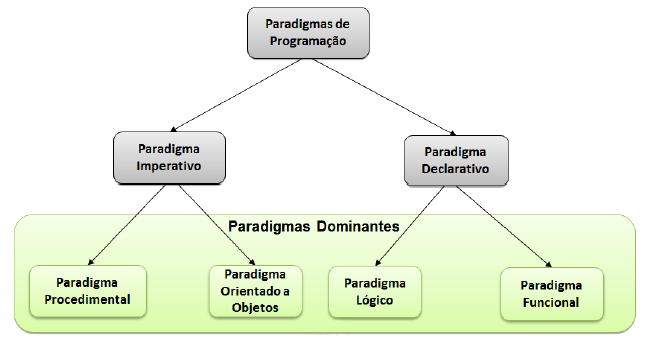
\includegraphics[width=0.85\textwidth]{../figures/classificacao_cut2.png}
  \fonte{Adaptado de \citeonline{doc_ronszcka_2019}}
  \label{fig:classificacao}
\end{figure}

Segundo Peter Van Roy, cada paradigma tem seu conjunto de técnicas e conceitos
de programação que, conjuntamente, definem sua forma de estruturar o pensamento
na construção de programas \cite{van_roy_2012}. Com base nesses conceitos ele
elaborou uma taxonomia para paradigmas de programação, conforme apresentada na
Figura \ref{fig:paradigmas_roy}. Neste diagrama os paradigmas de programação são
organizados em um grafo que apresenta o relacionamento conceitual entre eles.
Neste contexto, setas entre dois quadros representando paradigmas representam a
adição de novos conceitos, de forma que o paradigma derivado contempla os
conceitos dos paradigmas anteriores, acrescidos de um ou mais novos conceitos
que, conjuntamente, os definem como paradigmas distintos \cite{van_roy_2012}.

\begin{figure}[!htb]
  \centering
  \caption{Taxonomia dos paradigmas e linguagens}
  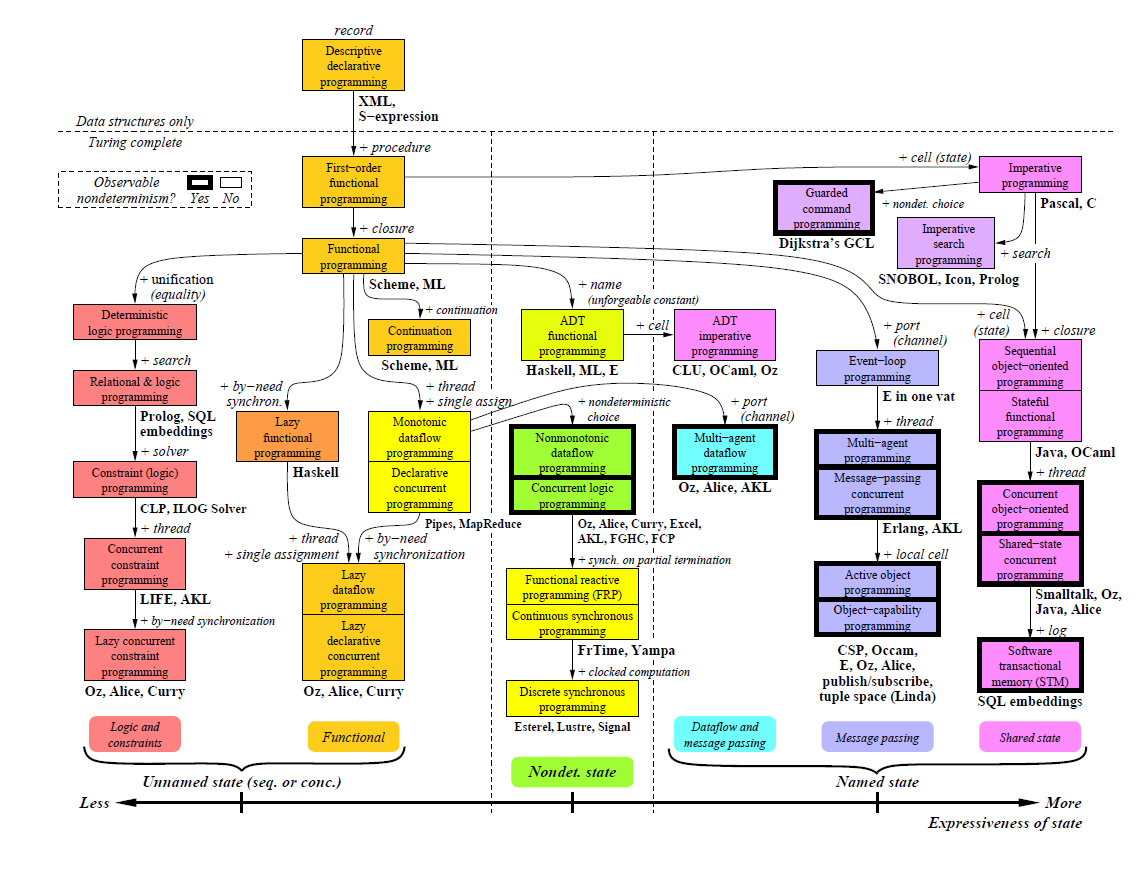
\includegraphics[width=\textwidth, height=0.46\textheight]{../figures/taxonomia.png}
  \fonte{\citeonline{van_roy_2012}}
  \label{fig:paradigmas_roy}
\end{figure}

Cada linguagem de programação materializa um ou mais paradigmas, sendo que cada
paradigma é composto por um conjunto de conceitos \cite{van_roy_2012}. Essa
relação entre as linguagens, paradigmas e conceitos é ilustrada na Figura
\ref{fig:concepts}. Na prática, quanto mais paradigmas de programação uma
linguagem suportar, melhor seria, pois, em dados termos isso provê ao
desenvolvedor um conjunto ainda maior de ferramentas. Em havendo mais
ferramentas, elas podem ser escolhidas para serem utilizadas de forma a melhor
se encaixar no problema específico, visto que nenhum paradigma por si só seria a
melhor solução para todos os problemas \cite{van_roy_2004}.

Em verdade, no desenvolvimento de uma única aplicação podem sim, ser
encontrados diversos paradigmas, sendo eles aplicados em partes individuais do
programa e fidedignas a cada paradigma empregado. Esse estilo de programação é
naturalmente chamado de multiparadigma. Entretanto e finalmente, a utilidade de
uma linguagem multiparadigmas depende naturalmente de quão bem os diferentes
paradigmas estão integrados \cite{bjarne_1995,van_roy_2004}.

\begin{figure}[!htb]
  \centering
  \caption{Linguagens, paradigmas e conceitos}
  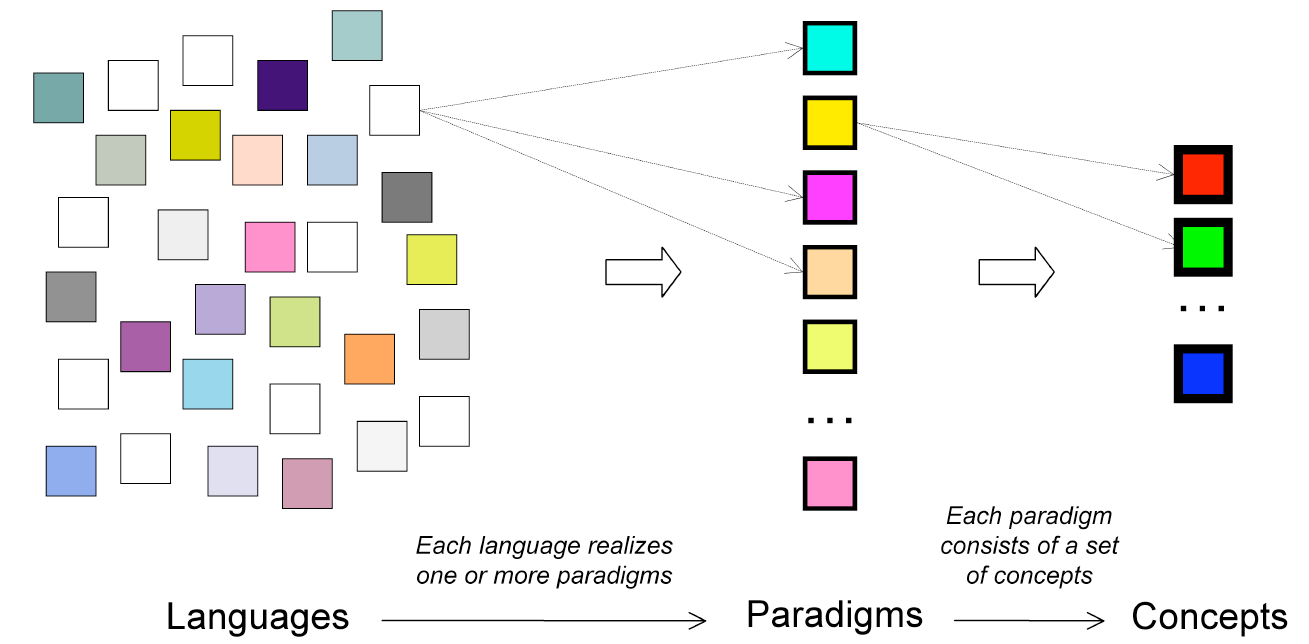
\includegraphics[width=0.85\textwidth]{../figures/concepts.png}
  \fonte{\citeonline{van_roy_2012}}
  \label{fig:concepts}
\end{figure}

Dentre os paradigmas dominantes citados, o POO está entre os mais utilizados.
Essa conclusão pode ser tirada ao se observar a Tabela \ref{tab:linguagens}, em
que 4 das 5 linguagens mais populares em 2021 materializam o POO (Java, Python,
C++ e C\#), somando um total de 35,07\% no Índice TIOBE\footnote{A sigla TIOBE
  vem de \textit{The Importance of Being Earnest} (\textit{i.e.}, A Importância de
  Ser Zeloso), título de uma peça de comédia de 1895 de Oscar Wilde, que é a
  inspiração para nome da companhia holandesa homônima que mantém o Índice TIOBE.}
da Comunidade de Programação \cite{tiobe_2021}. Essas linguagens são as
conhecidas Java, Python, C++ e C\#.

Em tempo, o Índice TIOBE é um indicador de popularidade de linguagens de
programação, atualizado mensalmente, utilizando dados disponíveis nas
ferramentas de pesquisa online. Este índice não reflete qualitativamente sobre
as linguagens de programação, mas sim quantitativamente sobre o volume de código
escrito com as mesmas.

\begin{table}[!htb]
  \centering
  \caption{Índice TIOBE de linguagens de programação}
  \smallskip
  \begin{tabularx}{0.3\textwidth}{|X|l|}
    \hline
    Linguagem & Índice  \\
    \hline
    C         & 12,54\% \\
    \hline
    Python    & 11,84\% \\
    \hline
    Java      & 11,54\% \\
    \hline
    C++       & 7,36\%  \\
    \hline
    C\#       & 4,33\%  \\
    \hline
  \end{tabularx}
  \fonte{Adaptado de \citeonline{tiobe_2021}}
  \label{tab:linguagens}

\end{table}

Além de suas vantagens técnicas, a dominância do POO entre os paradigmas pode
ser atribuída também aos sucessos comerciais das linguagens que os materializam,
à luz dos ganhos que a POO traz vis-à-vis ao PP, sendo justamente o PP o segundo
paradigma mais relevante neste mesmo índice de popularidade. Neste âmbito  do
domínio do POO, Java, C++ e Kotlin dominam o mercado de desenvolvimento Android,
enquanto Swift e Objective-C dominam o de iOS, de forma que é muito difícil
desenvolver \textit{software} para plataformas \textit{mobile} sem dominar o
POO. Da mesma forma, também tem se tornando importante conhecer o POO para o
desenvolvimento web, salientando aqui as linguagens JavaScript, Python e Ruby
\cite{gwosdz_2020}.

Dentre essas linguagens salientadas, destaca-se C++ em alguns aspectos, cuja
grande popularidade é atribuída por prover a velocidade de execução do C
enquanto dá suporte ao POO efetivamente, tendo permitido a transição do
PP para o POO por suportar ambos. De fato, desde a sua concepção, ela foi tida,
na verdade, como uma linguagem desenvolvida para suportar diversos estilos de
programação e, por sua vez, paradigmas, diferindo de linguagens que focam no
suporte de apenas um destes estilos \cite{bjarne_1995}. Com essa perspectiva de
ampliar o suporte a múltiplos paradigmas destaca-se a adição de expressões
lambda no padrão C++11, que ampliou o suporte do C++ ao paradigma de programação
funcional \cite{bjarne_2020}.

Mesmo uma linguagem como C++, entretanto, ainda herda os problemas de
sequencialidade da busca e orientação a pesquisas sobre elementos passivos por
meio de laços de repetição, advindo da computação sequencial. Na verdade, estes
problemas afetam desde linguagens imperativas até declarativas, sendo que estas
últimas, na prática, são implementadas com base nas primeiras finalmente,
conforme já discutido. Esses problemas trazem redundâncias temporais e
estruturais que podem causar prejuízos em desempenho e também em desacoplamento,
dificultando tanto a modularização do código como a execução de forma paralela
ou com paralelismos enfim, além da distribuída
\cite{simao_2009,simao_2012a,doc_ronszcka_2019}.

\subsection{Paradigmas de Programação Emergentes}\label{sec:intro_emergentes}

Conforme explicado anteriormente, o PP e o POO do PI e o PF e o PL do PD, são
conhecidos como Paradigmas Dominantes por estarem bem estabelecidos e em pleno
uso prático. Além dos Paradigmas Dominantes também existem diversos outros
paradigmas, ainda com menor grau de importância na prática industrial ou pelo
menos não ainda de mesmo impacto que os dominantes, dado que são propostas mais
recentes, mas que sim contribuem com novas formas de se conceber programas.

Estes novos paradigmas por sua vez são referenciados como Paradigmas Emergentes.
Dentre os Paradigmas Emergentes estão o Paradigma Orientado a Eventos (POE),
Paradigma Orientado a Componentes (POC), o Paradigma Orientado a Aspectos (POAs)
e o Paradigma Orientado a Agentes (POAg) \cite{msc_Banaszewski_2009}. A Figura
\ref{fig:emergentes} ilustra essa organização em Paradigmas Dominantes e
Emergentes, indicando justamente a precedência dos Paradigams Dominantes com
relação aos Paradigmas Emergentes.

\begin{figure}[!htb]
  \centering
  \caption{Classificação dos paradigmas de programação}
  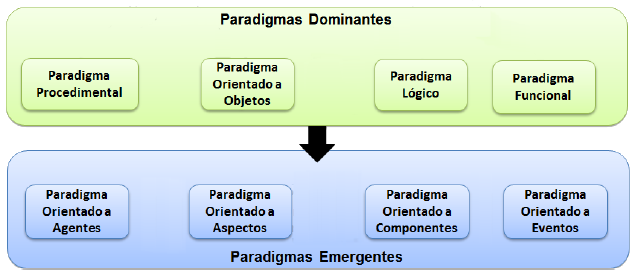
\includegraphics[width=0.85\textwidth]{../figures/classificacao_cut3.png}
  \fonte{Adaptado de \citeonline{doc_ronszcka_2019}}
  \label{fig:emergentes}
\end{figure}

Os ditos Paradigmas Dominantes já estão estabelecidos há muito tempo, como o PP,
cuja origem foi na década de 50, enquanto os ditos Paradigmas Emergentes, em sua
maior parte, têm sua concepção mais recente, após a década de 90. Neste
contexto, a Figura \ref{fig:evolucao} apresenta uma linha temporal com os
Paradigmas Dominantes, exemplificando com as linguagens de programação nas quais
os paradigmas são aplicados e mesmo os Emergentes. Isto permite entender por quê
os Paradigmas Emergentes apenas iniciam sua trajetória para alcançar maior
impacto na prática industrial \cite{msc_Banaszewski_2009}.

\begin{figure}[!htb]
  \centering
  \caption{Evolução dos paradigmas de programação}
  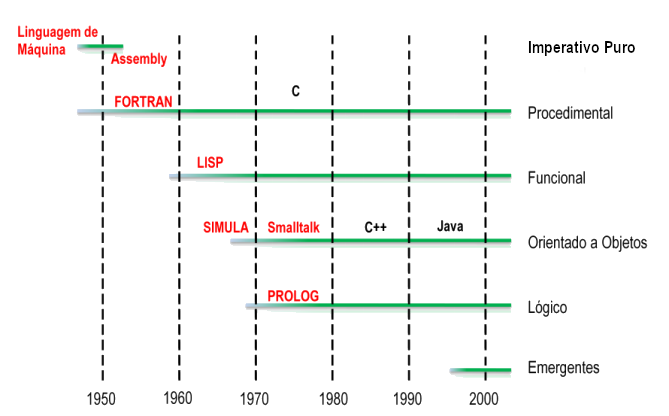
\includegraphics[width=0.8\textwidth]{../figures/evolucao.png}
  \fonte{Adaptado de \citeonline{msc_Banaszewski_2009}}
  \label{fig:evolucao}
\end{figure}

Os ditos Paradigmas Emergentes citados buscam propor soluções a problemas
existentes dos Paradigmas Dominantes, porém ainda herdam os problemas de
sequencialidade pela orientação a buscas/percorrimentos do PI e POO, já
mencionados, ainda que atenuados em certa medida no Paradigma Orientado a
Eventos (POE), devido à interação entre objetos que ocorre por meio de eventos,
alterando o fluxo de execução do programa \cite{ferg_2006}. O detalhamento tanto
do POE como dos outros paradigmas mencionados neste capítulo é feito na Seção
\ref{sec:paradigmas}.

\subsection{Paradigma Orientado a Notificações — PON}\label{sec:pon}

À luz do apresentado nas seções anteriores, é introduzido o Paradigma Orientado
a Notificações (PON). O PON pode ser inserido nesse contexto como um paradigma
emergente, mas \textit{sui generis}. O PON surge embrionariamente em 2001 por
meio da proposta de um metamodelo para a solução de problemas de controle
discreto, o qual evoluiu como uma solução geral de inferência. Subsequentemente,
a solução evolui para um paradigma de programação e mesmo de desenvolvimento em
geral
\cite{simao_livro_2002,doc_simao_2005,pat_simao_2008,simao_2009,doc_ronszcka_2019}.
O PON, como paradigma de programação/desenvolvimento, tem os objetivos de tornar
menos árdua a tarefa do desenvolvimento de sistemas por permitir concepção em
alto nível, tornar o código e sua execução mais eficiente por evitar
redundâncias (estruturais e temporais) e, por fim, tornar a sua execução
paralelizável/distribuível por garantir o desacoplamento \cite{simao_2009}.

O PON até encontra inspirações no PI, tais como a flexibilidade algorítmica e a
abstração em forma de objetos do POO e mesmo a reatividade da programação
dirigida a eventos, entretanto ambas postas de modo distinto. Ele também
até aproveita conceitos próprios do PD, como a facilidade de programação em alto
nível e a representação do conhecimento em regras, mas também com as suas
próprias idiossincrasias que o permitem ser algo outro. Assim, neste âmbito, o
PON provê a possibilidade do uso de partes de ambos os estilos de programação em
alguma medida, apresentando, contudo, revoluções em seu modelo no tocante aos seus
constituintes, à organização deles e ao seu processo de inferência ou cálculo
lógico-causal \cite{pat_simao_2008,simao_2009,doc_ronszcka_2019}.

Como o próprio nome sugere, a principal característica estrutural do PON é que
ele é construído com base em notificações entre as suas entidades
(\textit{i.e.}, \textit{Attributes}, \textit{Premises}, \textit{Conditions},
\textit{Rules}, \textit{Actions}, \textit{Instigations} e \textit{Methods}),
havendo, portanto, um mecanismo para tal. Cada elemento constituinte do PON pode
enviar e/ou receber notificações pontuais, fazendo com que as avaliações lógicas
e causais somente sejam realizadas quando ocorre uma notificação. Na verdade, o
PON propõe a divisão da computabilidade em dois grandes grupos de entidades, um
grupo facto-execucional e outro grupo lógico-causal, relacionados entre si por
meio de notificações de seus constituintes. O primeiro grupo se constitui dos
\textit{Fact Base Elements} (\textit{FBEs}), enquanto o segundo se constitui em
entidades chamadas de \textit{Rules}.

Em suma, \textit{FBEs} e \textit{Rules} se compõem de elementos menores que
permitem realizar o fluxo de notificações entre \textit{FBEs} e \textit{Rules} e
vice-versa. No PON, cada \textit{Rule} é a entidade capaz de tratar uma
expressão lógico-causal. Assim, as \textit{Rules} gerenciam o conhecimento sobre
qualquer comportamento lógico-causal no sistema. O conhecimento lógico-causal de
uma \textit{Rule} provém normalmente de uma regra se-então, o que é uma maneira
natural de expressão deste tipo de conhecimento. Por sua vez, o \textit{FBE} é
uma entidade usada para descrever estados e serviços de entidades reais ou
cibernéticas em um problema computacional \cite{msc_Banaszewski_2009}.

Na Figura \ref{fig:nop_rule}, é apresentado um exemplo de entidade
\textit{Rule}, justamente na forma de uma regra lógico-causal, já com a
indicação de suas entidades constituintes menores \cite{neves_icist_2021}. A
\textit{Rule} ilustrada seria parte de um sistema de tomada de decisão relativa
a um dado sensor. Este sensor compõe a etapa facto-execucional do sistema na
forma de um \textit{FBE}, enquanto a \textit{Rule} compõe a etapa lógico-causal.

\begin{figure}[!htb]
  \centering
  \caption{Estrutura de \textit{Rule} no PON}
  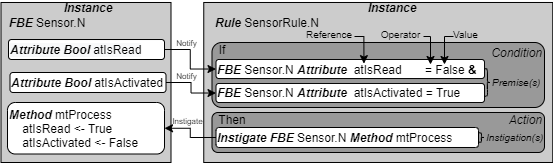
\includegraphics[width=0.95\textwidth]{../figures/rule_sensor_icist.png}
  \smallskip\smallskip\smallskip \fonte{\citeonline{neves_icist_2021}}
  \label{fig:nop_rule}
\end{figure}

Mais precisamente, o sensor é representado pelo \textit{FBE} \textit{Sensor} com
seu \textit{Method} \textit{mtProcess} e seus \textit{Attributes}
\textit{atIsRead} e \textit{atIsActivated}. A \textit{Rule}, por sua vez,
apresenta uma \textit{Condition} que é composta por duas \textit{Premises} que
fazem as seguintes verificações sobre o \textit{FBE}: a) \textit{O sensor foi
  lido?} b) \textit{O sensor foi ativado?}. A aprovação desta \textit{Condition}
leva a execução da \textit{Rule}, que por sua vez aciona a sua \textit{Action},
a qual é composta uma \textit{Instigation}. A aprovação da \textit{Rule} resulta
na execução do \textit{Method} \textit{mtProcess} que implementa a
funcionalidade de processar no \textit{FBE Sensor}, atribuindo valores aos seus
\textit{Attributes} que levam a mudança de estado de cada um deles.

Em suma, a \textit{Condition} da \textit{Rule} em questão lida com a decisão de
processamento do sensor a partir de duas \textit{Premises} que avaliam estados
dos \textit{Attributes} do \textit{FBE Sensor}. Uma vez que a decisão seja
positiva, a \textit{Action} da \textit{Rule} é responsável pela instigação da
\textit{Instigation}, a qual instiga o \textit{Method} da \textit{Rule}. Isto
posto, por generalização, percebe-se que todo o processamento lógico-causal e
facto-execucional é efetuado por elementos constituintes das \textit{Rules} e
\textit{FBEs}, tidos como entidades pequenas ou mínimas
\cite{pat_simao_2008,simao_2009,doc_Kerschbaumer_2018}.

O diagrama de classes da Figura \ref{fig:nop_class} apresenta as relações entre
todos os elementos do chamado metamodelo do PON
\cite{simao_2009,msc_Ronszcka_2012,simao_2012a}. Assim sendo, cada um dos
elementos constituintes do PON é mais precisamente e mesmo sucintamente
detalhado conforme segue:

\begin{itemize}
  \item \textit{Fact Base Element} (FBE): Entidade de \textit{Elemento Base de
          Fatos} que contém os \textit{Attributes} e \textit{Methods}, podendo ser
        considerada similar aos objetos do POO em termos simplistas.
  \item \textit{Attribute}: Entidade de \textit{Atributo} que representa, cada
        qual, uma propriedade de um \textit{FBE}, sendo responsável por armazenar um
        valor discreto-factual que representa estados. Um \textit{Attribute} difere de
        uma variável do PP ou atributo do POO tradicional no sentido de que possui a
        capacidade de notificar \textit{Premises} relacionadas quando seu estado é
        alterado.
  \item \textit{Premise}: Entidade de \textit{Premissa} que realiza a avaliação
        lógica de estados de dois \textit{Attributes} por meio de determinado operador
        de comparação (\textit{e.g.,} igual, diferente, maior e menor) e notifica
        \textit{Conditions} relacionadas quando muda de estado lógico.
  \item \textit{Condition}: Entidade de \textit{Condição}, que realiza a
        avaliação lógica de \textit{Premises} por meio de determinado operador lógico
        (\textit{e.g.,} conjunção ou disjunção), e notifica \textit{Rules} relacionadas
        quando muda de estado, como de aprovada para reprovada e vice-versa.
  \item \textit{Rule}: Entidade de \textit{Regra}, relacionada a uma
        \textit{Condition}. Tipicamente, cada \textit{Rule} executa sua \textit{Action}
        quando é aprovada.
  \item \textit{Action}: Entidade de \textit{Ação}, cada \textit{Rule} é
        relacionada a uma \textit{Action}, que se relaciona com uma ou mais
        \textit{Instigations}. Ela ativa todas as suas \textit{Instigations} quando é
        executada uma vez notificada pela \textit{Rule}.
  \item \textit{Instigation}: Entidade de \textit{Instigação}, responsável por
        instigar os \textit{Methods} relacionados quando é ativada pela \textit{Action}
        relacionada.
  \item \textit{Method}: Entidade de \textit{Método} do PON, de forma análoga a
        funções membro (ou métodos) do POO, sendo executado quando notificado/instigado
        pela \textit{Instigation}.
\end{itemize}

%\begin{figure}[!htb] \centering
%\caption{Estrutura do
%\textit{FBE} no PON} 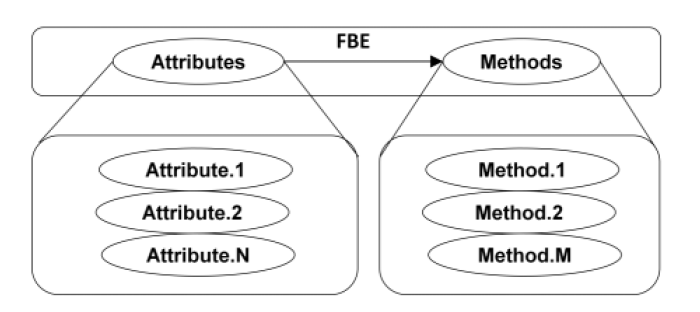
\includegraphics[width=0.6\textwidth]{../figures/fbe.png} \fonte{\citeonline{msc_Banaszewski_2009}}
%\label{fig:fbe} \end{figure}

\begin{comment}

O diagrama de classes da Figura \ref{fig:nop_class} apresenta as relações entre
todos os elementos do metamodelo do PON
\cite{simao_2009,msc_Ronszcka_2012,simao_2012a}. À luz deste metamodelo, uma
\textit{Rule} é composta por uma entidade \textit{Condition} e uma entidade
\textit{Action}. A \textit{Condition} trata da decisão da \textit{Rule}, enquanto
a \textit{Action} trata da execução das ações da \textit{Rule}. Assim,
\textit{Condition} e \textit{Action} trabalham para realizar o conhecimento
causal da \textit{Rule}. Na verdade, tanto a \textit{Condition} quanto a
\textit{Action} são entidades reativas agregadas nela
\cite{simao_2009,simao_2012a,doc_ronszcka_2019}.

\end{comment}

\begin{figure}[!htb]
  \centering
  \caption{Diagrama de classes das entidades do metamodelo do PON}
  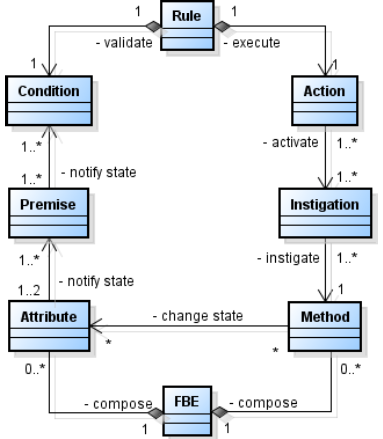
\includegraphics[width=0.6\textwidth]{../figures/metamodelo_pon.png}
  \fonte{\citeonline{msc_Ronszcka_2012}}
  \label{fig:nop_class}
\end{figure}

O fluxo de execução, ilustrado na Figura \ref{fig:nop_chain}, ocorre em função
da mudança de estado de um \textit{Attribute} de determinado \textit{FBE}. A
mudança de estado no \textit{Attribute} notifica as suas \textit{Premises}, que
por sua vez reavaliam os seus estados lógicos. Se o valor lógico da
\textit{Premise} se altera ocorre então uma notificação para as
\textit{Conditions} interessadas no estado desta \textit{Premise}.
Consequentemente, cada \textit{Condition} avalia seu valor lógico segundo as
\textit{Premises} relacionadas. Quando a condição da \textit{Condition} é
satisfeita, isto resulta na aprovação da sua respectiva \textit{Rule} para a
execução. Quando a \textit{Rule} é aprovada, sua \textit{Action} é ativada. Uma
\textit{Action} é conectada a uma ou mais \textit{Instigations}, que por sua vez
acionam a execução de alguma funcionalidade de um \textit{FBE} por meio dos seus
\textit{Methods}. As chamadas para um \textit{Method} podem causar alteração nos
estados dos \textit{Attributes} e o ciclo de notificação recomeça
\cite{msc_Banaszewski_2009}.

O fluxo de iterações das aplicações em PON é realizado por meio de uma cadeia de
notificações pontuais entre as entidades do PON. Essa cadeia de notificações é
transparente ao desenvolvedor, porque as notificações são realizadas de forma
autônoma pelas entidades reativas do PON. O fluxo de iterações do PON difere do
fluxo de iterações de aplicações do PI, no qual o desenvolvedor deve modelá-lo
de maneira explícita por meio do uso de laços de repetição. No PON esse fluxo
acontece de forma natural na perspectiva de execução da aplicação, conforme
exemplificado na Figura \ref{fig:nop_chain} e esboçado no diagrama de classes da
Figura \ref{fig:nop_class}.

\begin{figure}[!htb]
  \centering
  \caption{Representação do fluxo de notificações do PON}
  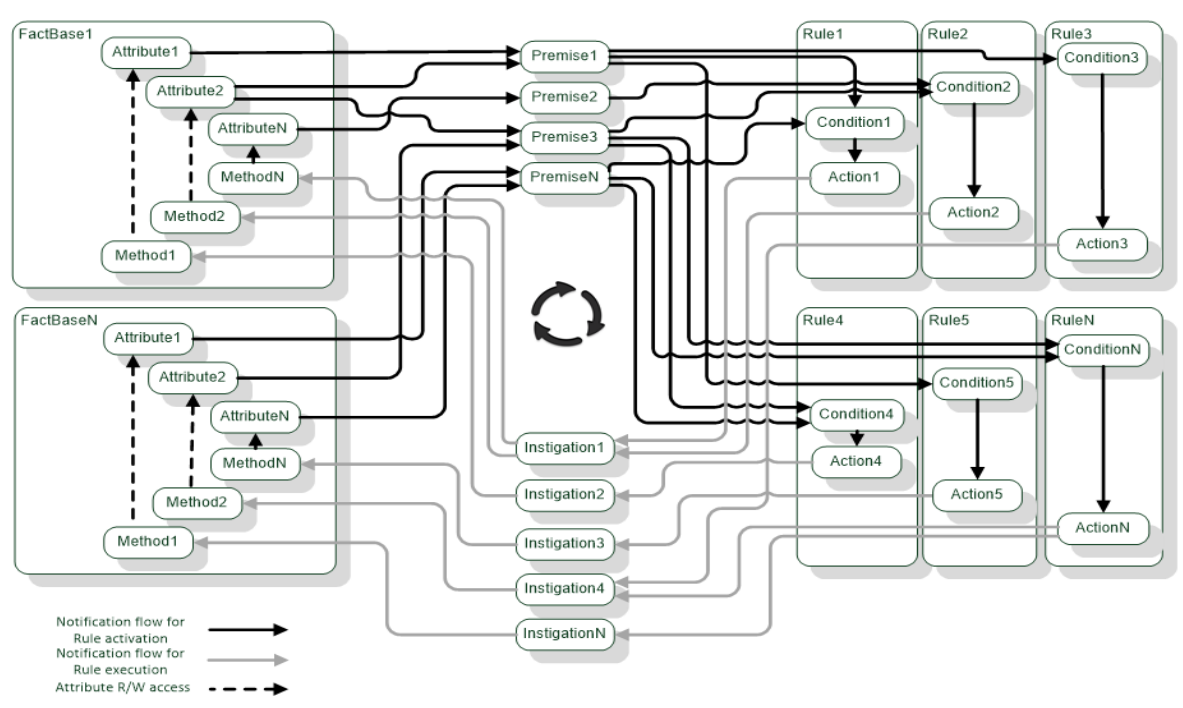
\includegraphics[width=\textwidth]{../figures/notificacoes_linhares.png}
  \smallskip
  \fonte{\citeonline{doc_linhares_2015}}
  \label{fig:nop_chain}
\end{figure}

No PON, as entidades pequenas são reativas e efetivamente desacopladas, sendo
que colaboram entre si por meio de notificações pontuais de modo a realizar o
cálculo lógico-causal de forma precisa, nos termos já explicados, evitando
implicitamente redundâncias de processamento. Essas notificações ditam,
portanto, o fluxo de execução das aplicações. Eis que essa nova maneira de
concepção de programas tende a proporcionar melhora no desempenho das
aplicações, potencialmente facilitando a sua concepção, tanto para ambientes não
distribuídos como para ambientes distribuídos
\cite{pat_simao_2008,simao_2009,simao_2012a}.

Esta seção introduz o PON de maneira breve, sendo que nas Seções
\ref{sec:estado_arte_pon}, \ref{sec:review} e \ref{sec:conceitos_pon} é feita
uma revisão mais aprofundada do estado da arte do PON. Além disso, o PON não
está vinculado a nenhuma plataforma específica, possuindo implementações em
diversas plataformas. Uma revisão detalhada sobre as diversas materializações
disponíveis do PON é feita na Seção \ref{sec:frameworks}.

No tocante às implementações em plataformas de \textit{software},
particularmente dos \textit{frameworks}, uma lacuna destes é a falta de uso
extensivo de programação genérica, bem como a falta de orientação a testes
ostensiva nos seus desenvolvimentos. Nesse sentido, a Seção \ref{sec:generic}
apresenta os conceitos de programação genérica que podem ser aplicados em
materializações do PON.

\subsection{Programação Genérica}\label{sec:generic}

A programação genérica pode ser caracterizada como uma técnica de programação
que foca na abstração dos seus algoritmos na sua forma mais genérica, mas sem
perda de eficiência \cite{stepanov_2015}. A aplicação das técnicas de
programação genérica consiste em escrever código que consegue suportar e atender
adequadamente diferentes tipos de dados, no qual o tipo é interpretado como um
argumento que só é de fato aplicado quando o código for instanciado utilizando
um tipo concreto \cite{stepanov_1998}.

Essa técnica é frequentemente utilizada para resolver um problema inerente de
linguagens de programação com tipagem estática, que é a pouca flexibilidade de
tipos em comparação com as linguagens com tipagem dinâmica \cite{cardelli_1985}.
Nas linguagens com tipagem estática, os tipos das variáveis são resolvidos na
etapa de compilação, enquanto nas linguagens com tipagem dinâmica os tipos são
resolvidos apenas durante a execução. Tem-se como exemplo o C++ enquanto uma
linguagem com tipagem estática, bem como a linguagem Python enquanto uma
linguagem com tipagem dinâmica \cite{hurd_2021}.

Mais precisamente, um problema clássico que a programação genérica resolve é a
duplicidade de código, principalmente em linguagens com tipagem estática. É
muito comum haver a necessidade de realizar operações ou algoritmos, por meio de
funções, utilizando variáveis de diversos tipos ao longo do código. Um exemplo
usual são estruturas de dados, como listas encadeadas, que atuam sobre entidades
computacionais de diversos tipos. Nesse tipo de caso, pode haver a duplicação de
código ao declarar funções diferentes, ainda que similares, para o tratamento de
cada tipo \cite{alexandrescu_2001,stepanov_2015}.

Os códigos e algoritmos desenvolvidos com programação genérica precisam,
entretanto, alcançar um desempenho tão bom quanto algoritmos escritos com código
em tipagem específica, caso contrário seria muito difícil justificar seu uso em
casos nos quais o desempenho seja uma característica importante
\cite{stepanov_2015}. A substituição dos tipos em tempo de compilação faz com
que o compilador gere o código especializado para cada tipo instanciado pelo
programa, de forma que tanto o desempenho como as propriedades fornecidas pela
tipagem estática são mantidas mesmo em um quadro de código genérico
\cite{alexandrescu_2001}. Neste âmbito, caso o compilador tente instanciar o
código genérico utilizando um operador ou conversão não suportada pelo tipo
instanciado isso vai resultar em um erro de compilação \cite{bos_2019}.

No caso do C++ em particular, o principal recurso utilizado para a aplicação de
programação genérica são os \textit{templates}. Com os \textit{templates},
declara-se um tipo genérico, o qual é utilizado na definição do código em
desenvolvimento. Subsequentemente, o compilador se encarrega de substituir os
tipos conforme as chamadas deste código sejam instanciadas utilizando tipos
específicos. Essa substituição de tipos é feita na etapa de compilação, de forma
que isso não causa prejuízos em desempenho \cite{alexandrescu_2001}.

Tendo como exemplo uma função simples em C++ que retorna o máximo entre dois
valores, enquanto em uma implementação regular seria necessário criar código
dedicado para cada tipo utilizado, pode-se ter uma função genérica utilizando
\textit{templates}. Tais exemplos são mostrados nos Códigos
\ref{cod:getmax_regular} e \ref{cod:getmax_template}, respectivamente. É
interessante observar que na implementação do Código \ref{cod:getmax_regular} o
código utilizado no corpo das duas funções é igual, enquanto a
implementação do Código \ref{cod:getmax_template} elimina este código repetido.

\noindent
\begin{minipage}{.45\textwidth}
  \begin{lstlisting}[caption = {Função \textit{GetMax} sem \textit{templates}},
    source = {Autoria própria},
    label = {cod:getmax_regular}]
    int GetMax(int a, int b) {
      return (a>b)? a:b;
    }
    
    float GetMax(float a, float b) {
      return (a>b)? a:b;
    }
    
    int main() {
      GetMax(1, 2);
      GetMax(1.5, 2.7);
      return 0;
    }
    \end{lstlisting}
\end{minipage}\hfill
\begin{minipage}{.45\textwidth}
  \begin{lstlisting}[caption = {Função \textit{GetMax} com \textit{templates}},
    source = {Autoria própria},
    label = {cod:getmax_template}]
    template <typename T>
    T GetMax(T a, T b) {
      return (a>b)? a:b;
    }
    
    int main() {
      GetMax(1, 2);
      GetMax(1.5, 2.7);
      return 0;
    }
    \end{lstlisting}
\end{minipage}

Além da utilização de \textit{templates} para a passagem de argumentos de
funções, também é possível utilizar \textit{templates} na construção de classes.
Desta forma é possível definir os tipos de variáveis membros como
\textit{templates}, possibilitando a reutilização de código. No exemplo do
Código \ref{cod:template_class} são definidas classes para a implementação de
uma lista simplesmente encadeada com tipo genérico.

\begin{lstlisting}[caption = {Classe genérica com \textit{templates}},
source = {Autoria própria},
label = {cod:template_class}]
template <typename T>
class ListItem {
  // Definição da classe
  T* item;
  T* next;
}

template <typename T>
class List {
  // Definição da classe
  ListItem<T> head;
};

List<Animal> list_of_animals;
List<Car> list_of_cars;
\end{lstlisting}

Outro exemplo é apresentado no Código \ref{cod:ex_generic_1}, onde classes
distintas realizam um processo de inicialização por meio do método
\textit{init()}. Considerando uma situação na qual as classes A, B e C não são
relacionadas, de modo que não seria pertinente a aplicação de herança do POO, e
que os métodos \textit{init()} sejam similares, porém não idênticos, pode haver
duplicação de código nos métodos \textit{init()}. Neste caso pode ser feita a
aplicação de programação genérica para implementar parte destas funcionalidades
comuns, conforme apresentado no Código \ref{cod:ex_generic_2}. Desta forma, é
possível eliminar a duplicação de código desnecessária, sem haver quebra de
conceitos como herança \cite{thorsen_2015}. Em um programa sem a aplicação de
programação genérica seria necessário escrever o mesmo código duas vezes. Isso
traz o problema de duplicar o esforço gasto escrevendo código, assim como abre
espaço para o aparecimento de problemas futuros, pois a partir desse momento
será necessário fazer a manutenção de dois códigos separados. Portanto, podem
acabar surgindo defeitos em um ou outro, e eventualmente esses códigos podem
acabar divergindo e apresentando comportamentos diferentes, o que não seria o
desejado pela solução inicial \cite{stepanov_2015}.

\noindent
\begin{minipage}{.45\textwidth}
  \begin{lstlisting}[caption = {Exemplo de código sem programação genérica},
source = {Adaptado de \citeonline{thorsen_2015}},
label = {cod:ex_generic_1}]
class A {
    void init() {
        // Longo trecho de código complexo;
    };
};
class B { 
  void init() {
        // Similar ao init() de A 
  };
};
class C { 
  void init() {
        // Similar ao init() de A 
  };
};
\end{lstlisting}
\end{minipage}\hfill
\begin{minipage}{.45\textwidth}
  \begin{lstlisting}[caption = {Exemplo de código com programação genérica},
source = {Adaptado de \citeonline{thorsen_2015}},
label = {cod:ex_generic_2}]
template static inline void f1(T* t) {
    // Faz parte do trabalho de init()
    t->doSomething();
}
template static inline void f2(T* t) {
    // Faz outra parte do trabalho de init()
}
template static inline void f3(T* t) {
    // Faz outra parte do trabalho de init()
}
...
void A::init() {
	f1(this);
	f2(this);
	f3(this);
}
void B::init() { // Não utiliza f1
	f2(this);
	f3(this);
}
void C::init() { // Não utiliza f2
	f1(this);
	f3(this);
}
\end{lstlisting}
\end{minipage}

Na linguagem de programação C++ existe a biblioteca \textit{Standard Template
  Library} (STL), o que se constitui em um importante recurso nesta linguagem. A
STL é a biblioteca padrão de \textit{templates} que, dentre outros recursos,
contém definições de estruturas e algoritmos genéricos implementados com
\textit{templates}. Dentre esses, podemos citar as estruturas de listas,
vetores e algoritmos de ordenação e busca \cite{iso_cpp17}.

De forma geral, é dito que a programação genérica deve ser utilizada sempre que
possível, visto que reduz a duplicidade de código \cite{alexandrescu_2001}.
Porém, como contraponto, ela resulta em um código que é mais complexo, podendo causar
dificuldades para programadores iniciantes, que não tenham um domínio tão
completo da linguagem e que, portanto, apresentarão maior dificuldade em entender
essas construções genéricas mais complexas \cite{stepanov_2015}.

O suporte à programação genérica foi ampliado nas versões mais atuais do padrão
da linguagem de programação C++, com a adição de novos recursos, como
\textit{variadic templates} e \textit{fold expressions}
\cite{grimm_2020,bjarne_2020}. Em suma \textit{variadic templates} permitem a
utilização de \textit{templates} para a declaração de funções e métodos que
recebem um número variável de argumentos, enquanto as \textit{fold expressions}
fornecem os mecanismos necessários para se operar sobre esses conjuntos de
argumentos variáveis. Na Seção \ref{sec:cpp_moderno} são explorados com maiores
detalhes os recursos utilizados no escopo deste trabalho, incluindo
\textit{variadic templates} e \textit{fold expressions}.

Dado esse contexto é possível destacar que estes conceitos de programação
genérica podem ser aplicados no desenvolvimento dos \textit{frameworks} do PON
em C++ de modo a permitir maior flexibilidade de tipos e flexibilidade
algorítmica. A aplicação destes conceitos pode contribuir principalmente no
sentido de facilitar a programação em alto nível. A falta disto se constitui em
uma das imperfeições dos atuais \textit{frameworks} do PON. 

Outrossim, outra imperfeição seria a falta de ostensivo desenvolvimento
orientado a testes nos \textit{frameworks}. A carência da realização de testes
no processo de desenvolvimento das materializações atuais resulta em
dificuldades relativas ao seu uso principalmente no que diz respeito a presença
de problemas no código (\textit{i.e.}, \textit{bugs}) que são percebidos apenas
durante a sua utilização como, por exemplo, no caso do \textit{Framework} PON
C++ 2.0 conforme relatado por \citeonline{msc_xavier_2014} e no caso do
\textit{Framework} PON C++ 3.0 conforme relatado por
\citeonline{doc_Schutz_2019}

\subsection{Desenvolvimento Orientado a Testes — \textit{Test Driven
    Development} (TDD)}\label{sec:tdd_intro}

O método de desenvolvimento chamado Desenvolvimento Orientado a Testes ou, em
idioma inglês, o assim chamado \textit{Test Driven Development} (TDD), surgiu no
final da década de 90 \cite{test_driven_2013}, tendo seu ciclo de
desenvolvimento formal estabelecido por \citeonline{beck_2002}. O TDD é um
método que permite aumentar a confiabilidade do \textit{software}, por meio do
desenvolvimento de testes.

Como este presente trabalho envolve o desenvolvimento de um novo \textit{framework}
para PON em C++ (a chamada versão 4.0), inclusive com maior generalidade e
também com maior confiabilidade, há de se ter uma forma de reduzir o número
problemas encontrados durante seu uso e execução. Neste âmbito, a aplicação do
TDD se torna pertinente a este trabalho.

O uso de TDD evitaria enfim reincorrer em problemas no desenvolvimento de
\textit{frameworks} precedentes do PON, como erros de execução e retrabalho para
localizar a falha e alcançar as correções devidas. Por exemplo, há um erro
reportado no \textit{Framework} PON C++ 2.0 em \citeonline{msc_xavier_2014} que
só foi resolvido subsequentemente no \textit{Framework} PON C++ 3.0 em
\citeonline{belmonte_2012}, que por sua vez tinha imperfeições
tratadas apenas em \citeonline{doc_Schutz_2019}.

Isto dito, o método do TDD transforma o processo de desenvolvimento do
\textit{software}, dando maior foco ao desenvolvimento dos testes. Uma concepção
equivocada, porém muito comum, do TDD é que todos os testes devem ser
desenvolvidos de uma única vez no começo da etapa de desenvolvimento.
Entretanto, na aplicação correta deste método, é dado foco ao desenvolvimento de
um teste por vez \cite{test_driven_2013}.

No ciclo de desenvolvimento estabelecido pelo TDD tem-se em primeiro lugar o
desenvolvimento de um teste para a funcionalidade que se deseja implementar.
Inicialmente a execução deste teste deve falhar, visto que a funcionalidade
ainda não foi implementada. Após a falha inicial do teste é feita a
implementação do código e então os testes são executados novamente. Esse ciclo
se repete até que todos os testes passem e enfim pode ser dado início ao ciclo
de implementação de uma nova funcionalidade \cite{ambler_2006}. Esse fluxo é
ilustrado na Figura \ref{fig:tdd_flow}.

\begin{figure}[!htb]
  \centering
  \caption{Fluxo de desenvolvimento no TDD}
  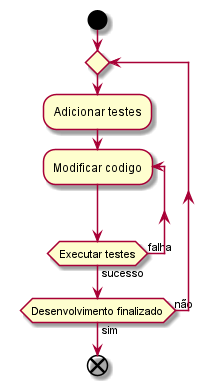
\includegraphics[width=.33\textwidth]{../out/diagrams/tdd/tdd.png}
  \smallskip
  \fonte{Adaptado de \citeonline{mody_2017}}
  \label{fig:tdd_flow}
\end{figure}

Nesse contexto, o TDD recorre a dois tipos de testes, os testes unitários e
testes de integração \cite{ambler_2006}. Os testes unitários são aqueles que
avaliam o funcionamento de uma unidade do código (como classes, objetos ou
funções), enquanto os testes de integração avaliam o funcionamento de diferentes
partes do sistema operando juntas. Em todo caso, para ambos os tipos de teste,
aplica-se o ciclo ilustrado na Figura \ref{fig:tdd_flow}.

Um dos principais benefícios desse método é que, uma vez que os testes já foram
desenvolvidos, torna-se possível garantir que a implementação de novas
funcionalidades não altera as funcionalidades já existentes no sistema, que
foram previamente testadas, contanto que os testes continuem sendo executados
com sucesso. O TDD também ajuda o desenvolvedor a detectar problemas na
arquitetura do \textit{software} durante o desenvolvimento
\cite{test_driven_2013}.

Em contraponto aos benefícios anteriormente apresentados, uma das maiores
dificuldades para a adoção do TDD no processo de desenvolvimento de
\textit{software} é que os inúmeros ciclos de desenvolvimento de testes e
desenvolvimento de código tendem a aumentar significativamente o tempo de
desenvolvimento. Entretanto, certamente, esse tempo gasto na etapa de
desenvolvimento é compensado pelo tempo economizado corrigindo problemas de
código durante a execução do \textit{software} desenvolvido
\cite{test_driven_2013}.

Devido a esse grande número de iterações de testes que acontecem durante o
processo, é essencial que os testes sejam fáceis de executar e também rápidos,
pois caso isto não ocorra esse processo pode consumir muito tempo durante o
desenvolvimento, no limite inviabilizando TDD \cite{test_driven_2013}. Assim,
para auxiliar neste processo, existem diversas ferramentas que podem auxiliar o
desenvolvedor, sendo que na Seção \ref{sec:test_frameworks} são apresentados
\textit{frameworks} para a realização de testes em C++.

Em suma, a aplicação do TDD no contexto do desenvolvimento de um novo
\textit{framework} do PON é importante, pois, conforme já explicado, permite
garantir a estabilidade do \textit{software} desenvolvido. Isso contribui para
melhorar a experiência de uso do \textit{framework} e, por tanto, do paradigma,
pois reduziria significativamente o número de problemas encontrados durante o
uso do mesmo por outros desenvolvedores.

\section{Motivação}\label{sec:motiv}

% As características e propriedades do Paradigma Orientado a Notificações (PON)
% apresentadas na Seção \ref{sec:pon} são interessantes ao 

% Essas necessidades se apresentam como uma motivação para a materialização do
% PON \cite{doc_ronszcka_2019}.

Os sistemas computacionais estão se tornando cada vez mais complexos ao longo
dos anos, exigindo cada vez mais soluções em \textit{software} e
\textit{hardware} que atendam às suas necessidades \cite{chien_2011,
quali_pordeus_2020}. Dentre as principais demandas contemporâneas e históricas
do desenvolvimento de \textit{software} está o desenvolvimento de programas em
alto nível, utilizando ferramentas que facilitem o processo de desenvolvimento.
Ademais, em simultâneo, almeja-se que tais programas apresentem alto desempenho,
com baixos tempos de execução. Por fim, eles deveriam ainda se adequar a
arquiteturas de computação modernas, como é o caso de arquiteturas de computação
\textit{multicore}, de forma a aproveitar seu potencial de paralelismo
\cite{belmonte_2016}.

Do ponto de vista de \textit{hardware}, mais especificamente, houve substancial
evolução no aspecto da integração de circuitos, sendo que no desenvolvimento de
processadores integram-se múltiplos núcleos em uma única pastilha, o que se
constitui nos processadores \textit{multicore} justamente
\cite{asanovic_2009,chien_2011, quali_pordeus_2020}. Nesse âmbito, de modo a
atingir alto desempenho, é necessário que o desenvolvimento de \textit{software}
seja capaz de fazer proveito da capacidade de paralelismo oferecida por tais
processadores, \textit{i.e.}, paralelizando \textit{threads} com granularidade
apropriada para tal
\cite{henessy_2003,doc_linhares_2015,belmonte_2016,msc_negrini_2019}.

Nesse contexto todo, considerando as características apresentadas na Seção
\ref{sec:pon}, o PON se apresenta como uma alternativa viável para o atendimento
destas demandas contemporâneas e históricas do desenvolvimento de
\textit{software}. À luz de sua teoria, as materializações em PON podem ser
evoluídas e utilizadas de forma a permitir o desenvolvimento de
\textit{software} em alto nível e com alto desempenho. O desenvolvimento de
\textit{software} em PON pode trazer benefícios como redução dos custos em tempo
de desenvolvimento ao permitir a programação em alto nível, ao mesmo tempo que
apresentaria desempenho compatível ou superior ao das tecnologias atualmente
utilizadas. Ademais, o alto nível de desacoplamento das entidades computacionais
em PON seria um facilitador para fins de paralelismo e/ou distribuição
\cite{simao_2012a,ronszcka_2017,doc_ronszcka_2019}.

Durante os últimos anos, o PON vem apresentando muitas evoluções, tanto do ponto
de vista do estado da arte, com o refinamento dos conceitos que formam o
paradigma, assim como do ponto de vista do estado da técnica. Dentre as
evoluções técnicas, está o desenvolvimento de \textit{frameworks} que
possibilitam a aplicação do paradigma em diversas linguagens de programação como
C++ \cite{msc_Banaszewski_2009,msc_Ronszcka_2012}, Java \cite{henzen_2015}, C\#
\cite{henzen_2015,msc_oliveira_2019}, Elixir/Erlang \cite{msc_negrini_2019}, bem
como por meio de linguagens ainda prototipais de programação próprias ao PON no
âmbito da chamada Tecnologia LingPON \cite{doc_ronszcka_2019}. Esses trabalhos
do estado da arte/técnica são explorados com mais detalhes na seção
\ref{sec:estado_arte_pon}, sendo salientados os \textit{frameworks} por serem
versões assaz estáveis, constituindo o estado da técnica enfim.

Ainda no âmbito do estado da técnica, eis que o paralelismo, justamente uma das
principais características do PON, não é implementada em certas versões de
\textit{framework}, particularmente naqueles em C++ e tampouco naqueles em C\# e
Java \cite{doc_ronszcka_2019}. Mais precisamente, isto é bem o caso do
\textit{Framework} PON C++ 1.0 e também do contemporâneo \textit{Framework} PON
C++ 2.0. Ainda, mesmo no \textit{Framework} PON C++ 3.0, que justamente visava
paralelismo ao nível de \textit{thread}, isto não é adequadamente ou, ao menos,
estavelmente implementado \cite{doc_ronszcka_2019,doc_Schutz_2019}. Por outro
lado, \textit{frameworks} PON que tratam mais apropriadamente deste tipo de
paralelismo, como \textit{Framework} Akka e \textit{Framework} Elixir/Erlang,
usam linguagens de nível muito alto (orientada a atores) que não primam pelo
alto desempenho, como ocorreria se fossem feitos em C++
\cite{doc_ronszcka_2019,msc_negrini_2019,negrini_2019,negrini_2019_2}.

Assim sendo, uma versão nova de \textit{framework}, do PON que resolvesse
imperfeições dos precedentes e tivesse usabilidade melhorada, facilitaria o
aprendizado e aplicação dos conceitos deste paradigma emergente. Esta nova
versão também poderia potencialmente aumentar o volume e qualidade das
aplicações desenvolvidas neste paradigma, por meio da natural redução do tempo
de desenvolvimento necessário para utilizar o \textit{framework}. Para tal, mais
pontualmente, o novo \textit{framework} deve ser mais versátil, inclusive
facilitando a integração com bibliotecas e aplicações externas, permitindo o uso
de programação genérica e tendo sido desenvolvido à luz de TDD. Quanto maior for
a maturidade das materializações do estado da técnica em PON e maior for a
facilidade de uso, maior será também a viabilidade do PON, auxiliando assim que
este evolua do estágio de Paradigma Emergente, no sentindo de começar a alcançar
a transição para um paradigma estabelecido, quiçá um dia tornando-se um
paradigma vigente.

Ainda no que diz respeito ao desempenho das aplicações, as materializações do
PON carecem de aplicações bem definidas que sirvam como \textit{benchmark} bem
estabelecido, permitindo a realização de comparações entre os
\textit{frameworks} do PON e até mesmo com outros paradigmas. Nesse contexto,
\citeonline{quali_pordeus_2020} propõe a utilização de dois algoritmos
conhecidos, o \textit{Random Forest} (que se trata de um algoritmo de
aprendizagem de máquina) e o \textit{Bitonic Sort} (um algoritmo de ordenação),
que permitiram a avaliação do desempenho do PON em ambientes \textit{mono} e
\textit{multicore}. De modo similar, \citeonline{msc_negrini_2019} também propõe
a implementação de algoritmos para o controle automatizado de tráfego. Com esse propósito,
uma versão nova de \textit{framework} do PON deveria ser capaz de implementar
tais aplicações propostas, se beneficiando também da utilização de ferramentas
que permitissem garantir a confiabilidade e reprodutibilidade destes resultados,
como por meio do uso de \textit{frameworks} de teste.

\section{Justificativa}

A principal forma disponível e tecnologicamente estável para o desenvolvimento
de aplicações no PON ainda é por meio do uso de \textit{frameworks}. Dentre
todas as materializações de \textit{frameworks} do PON, aquela que apresenta
maior grau de maturidade e estabilidade é o \textit{Framework} PON C++ 2.0
\cite{ronszcka_2017}. Apesar de todos os esforços já realizados no
desenvolvimento dos \textit{frameworks}, inclusive no \textit{Framework} PON C++
2.0, estes \textit{frameworks} ainda possuem muitas imperfeições e mesmo
deficiências. Isto foi, em partes, supra considerado e relatado neste trabalho.

Apesar dos \textit{frameworks} PON em C++ entregarem, do ponto de vista
conceitual, toda a funcionalidade necessária para o desenvolvimento de
aplicações em PON, eles ainda apresentam algumas limitações importantes, como
verbosidade, baixa flexibilidade de tipos, baixa flexibilidade algorítmica, além
de particularmente não contemplarem todas as propriedades elementares do PON.
Neste sentido, o \textit{Framework} PON C++ 2.0 não contempla a propriedade de
paralelismo, enquanto a programação em alto nível não é plenamente possível
devido principalmente à excessiva verbosidade de expressão de código imposta por
ele. O \textit{Framework} PON C++ 3.0, por sua vez, tenta materializar a
propriedade de paralelismo ao nível de \textit{thread}, porém não o faz de
maneira satisfatória, apresentando diversos problemas de estabilidade, conforme
reportado em \citeonline{doc_Schutz_2019} e outros
\cite{martini_2019,doc_ronszcka_2019,msc_negrini_2019}.

Além dos \textit{frameworks} em C++, os demais \textit{frameworks} também ainda
não atendem de forma satisfatória as demandas mencionadas na Seção
\ref{sec:motiv}. Os \textit{frameworks} em Java/C\# são versões prototipais e
sem contemplar paralelismo, enquanto as materializações em Elixir/Erlang e Akka
contemplam paralelismo, mas não possuem o desempenho apropriado possibilitado
pelas linguagens de mais baixo nível. Neste contexto, as propriedades atingidas
pelos \textit{frameworks} do PON são resumidas na Tabela \ref{tab:demandas}.

Os \textit{frameworks} C++ 2.0, C++ 3.0 e Java/C\# possuem o melhor desempenho
dentre os \textit{frameworks} do PON. Em termos de tempo de execução, devido à
implementação dos \textit{frameworks} em geral usando estruturas de dados
baseadas em linguagens do \textit{POO}, isto gera sobrecarga ou
\textit{overheads} que distanciam esta implementação do PON de sua teoria, com
cálculos assintóticos na ordem de \(O(n)\) para o caso médio e \(O(n3)\) para o
pior caso. No caso dos \textit{frameworks}, em determinados cenários, o
desempenho ainda é inferior quando comparado a aplicações implementadas
diretamente no \textit{POO}. Entretanto, é justamente nos \textit{frameworks} em
C++ que, em geral, os resultados ficam próximos ao de POO, ainda que não sempre
o superando como prevê a teoria, mas sim mantendo programação em mais alto nível
e com alto nível de desacoplamento ademais
\cite{msc_Banaszewski_2009,msc_valenca_2012}.

\begin{table}[!htb]
  \centering
  \caption{Propriedades do PON materializadas pelos \textit{frameworks} do PON}
  \smallskip
  \begin{tabularx}{\textwidth}{|l||*{6}{X|}}\hline
    \diagbox{Propriedade}{\textit{Framework}} & C++ 2.0    & C++ 3.0    & Java/C\#   & C\# IoT    &
    Elixir                                & Akka                                                                        \\\hline\hline
    Programação em alto nível             &            &            &            & \checkmark & \checkmark & \checkmark \\ \hline
    Paralelismo                           &            & \checkmark &            & \checkmark & \checkmark & \checkmark \\ \hline
    Desempenho                            & \checkmark &            & \checkmark &            &            &            \\ \hline
  \end{tabularx}
  \fonte{Autoria própria}
  \label{tab:demandas}
\end{table}

Dadas estas demandas, é possível constatar que existe a necessidade de uma
materialização que contemple essas demandas de forma mais satisfatória. Conforme
já salientado, os \textit{frameworks} em C++ tendem a ter melhor desempenho
quando comparado aos outros \textit{frameworks} do PON, entretanto ainda falta
neles maior facilidade de programação concorrente e distribuída, assim como de
programação genérica. Entretanto, parte das limitações e problemas existentes no
\textit{Framework} PON C++ 2.0 e \textit{Framework} PON C++ 3.0 podem ser
considerados decorrentes das limitações da tecnologia utilizada em suas
implementações, mais precisamente, o padrão C++98 da linguagem de programação
C++. Nesse âmbito, as inovações introduzidas nos padrões mais novos do C++,
principalmente o C++17 e C++20, podem contribuir para possibilitar o
desenvolvimento de um \textit{framework} capaz de atender a todas essas
demandas.

Dado ao excelente equilíbrio entre nível apropriado de abstração e desempenho
apropriado, o C++ é uma linguagem de programação apropriada para se realizar a
materialização do PON. Conforme constatado em \citeonline{tiobe_2021}, o C++
continua sendo uma linguagem de programação popular, ademais. Naturalmente, a
possibilidade de se utilizar o PON em uma linguagem de programação popular
facilitaria a aceitação dele por parte de novos desenvolvedores. Adicionalmente,
isto também permitiria a integração com outros programas e bibliotecas já
existentes em C++ e associados, de forma mais simples, assim possibilitando o
desenvolvimento de aplicações completas.

Ainda, apesar do C++ ser tradicionalmente uma linguagem de programação mais
usada no contexto da orientação a objetos, novos recursos adicionados nas suas
revisões mais recentes facilitam a programação funcional, por meio do uso das
expressões \textit{lambda} \cite{bjarne_2020}. Isto pode ser muito bem utilizado
em materializações do PON em C++  ara prover maior nível de flexibilidade de
programação (facto-execucional). Neste sentido de flexibilizações, com a
aplicação da programação genérica do C++ é possível atingir a flexibilidade de
tipos no \textit{framework}. Enquanto no \textit{Framework} PON C++ 2.0 se
precisava definir e implementar estruturas novas para cada tipo de dado a ser
utilizado (como \textit{int}, \textit{double}, \textit{string} e \textit{bool}),
em versão orientada a \textit{templates}/gabaritos seria possível utilizar
qualquer tipo de dado, pois as interfaces serão genéricas, não sendo necessário
código específico para implementar um tratamento diferente para cada tipo de
dado de entrada.

Outra melhoria que pode ser obtida ao se aplicar a programação genérica é
possibilitar reduzir a quantidade de código necessária para se compor o
\textit{framework} em si. Isso traz benefícios, como facilitar a manutenção do
código por outros desenvolvedores e/ou pesquisadores, possibilitando assim uma
melhor evolução do \textit{framework}. Facilitar-se-ia adicionar novos recursos
por não se fazer necessário reescrever uma grande quantidade de código. Ademais,
as contribuições da aplicação de programação genérica permitiriam ainda o
desenvolvimento de interfaces mais flexíveis e fáceis de utilizar, no sentido de favorecer a
programação em alto nível.

Por fim, com o C++17 também foram introduzidos mecanismos que facilitam a
programação concorrente, provenientes de mecanismos de execução paralela, como o
conceito de políticas de execução\footnote{As políticas de execução em C++
permitem especificar se a execução de algoritmos e laços de repetição deve ser
executada de forma sequencial ou paralela, esse conceito é explorado em maiores
detalhes na Seção \ref{sec:cpp_moderno}}. Esses mecanismos, enquanto recursos
nativos da linguagem, tornam transparente ao desenvolvedor a paralelização da
execução de \textit{threads} do \textit{software}, o que vai ao encontro do PON
no sentido de permitir \textit{threads} com granularidade fina. Esses recursos
permitiriam contornar a deficiência do \textit{Framework} PON C++ 3.0 no que diz
respeito à estabilidade, conforme reportado inclusive em
\citeonline{martini_2019}. Por agora serem recursos nativos da linguagem
C++, estes mecanismos naturalmente apresentam maior estabilidade que
implementações customizadas de paralelização, como a desenvolvida no
\textit{Framework} PON C++ 3.0.

Desta forma, em suma, observa-se que é factível o desenvolvimento de uma versão de
\textit{framework} em C++ melhor que atenda as propriedades do PON e, portanto,
vá ao encontro de todas as demandas de desenvolvimento de \textit{software} supra
apresentadas. Em suma, a programação genérica poderia ser utilizada para
facilitar a programação em alto nível, o bom desempenho já observado nas
materializações de \textit{frameworks} do PON em C++ existentes seria mantido e
quiçá melhorado e, por fim, as políticas de execução poderiam ser utilizadas
para implementar o suporte ao paralelismo de forma simples e estável.

Apesar da maturidade e estabilidade apresentadas pelo \textit{Framework} PON C++
2.0, as limitações impostas pelas tecnologias utilizadas em sua implementação,
como o antigo padrão C++98 da linguagem C++, a excessiva verbosidade e grande
quantidade de código redundante dificultam a implementação de melhorias sobre
sua base de código. Desta forma, em suma, há espaço para a implementação de uma
nova materialização de \textit{framework}, a qual deve ser desenvolvida fazendo
proveito dos avanços no estado da técnica introduzidos pelos \textit{frameworks}
já disponíveis, porém realizando implementações mais apropriadas em termos de
programação contemporânea de \textit{software} aplicando as melhorias acima
propostas.

Além disso, a implementação de determinadas aplicações, como os
\textit{benchmarks} propostos por \citeonline{pordeus_2020} por meio dos
algoritmos \textit{Random Forest} e \textit{Bitonic Sort} são difíceis, ou quiçá
impossíveis, de serem implementados de forma satisfatória com o
\textit{Framework} PON C++ 2.0. O \textit{Random Forest} é um algoritmo de
aprendizagem de máquina, que pode se beneficiar da paralelização da execução de
suas árvores de decisão, o que não seria contemplado por implementações com o
\textit{Framework} PON C++ 2.0. Por sua vez, o \textit{Bitonic Sort} é um
algoritmo de ordenação, sendo composto por várias etapas de decisão avaliando
elementos dois a dois, que podem ser implementadas por várias \textit{Rules} do
PON, o qual seria difícil de implementar com o \textit{Framework} PON C++ 2.0
devido à complexidade da inicialização de suas entidades. Nesse sentido, a
implementação de um novo \textit{framework} do PON possibilitaria a realização
destes \textit{benchmarks}.

\section{Objetivo geral}\label{sec:obj_geral}

O objetivo geral deste trabalho é promover avanços ao Paradigma Orientado a
Notificações (PON) via um novo \textit{framework} orientado a TDD, programação
genérica e recursos modernos da linguagem de programação C++20 (\textit{single
thread} e \textit{multithread}), para melhor contemplar as propriedades
elementares do PON no estado da técnica, o que deve ser validado via
\textit{benchmarks} apropriados (\textit{e.g.}, \textit{biotonic} e
\textit{random forest}).

\section{Objetivos específicos}\label{sec:obj_especificos}

Para atingir o objetivo geral, este trabalho apresenta os seguintes objetivos
específicos:

\newcommand{\SubItem}[1]{
    {\setlength\itemindent{15pt} \item[-] #1}
}
\begin{itemize}
  %\item Dissertar sobre as materializações do PON, fazendo as devidas críticas
  %(como a falta de programação genérica e \textit{multithread} efetivo em
  %materializações em C++) e propondo melhorias a serem contemplados na nova
  %versão de \textit{framework} PON C++. \item Realizar um levantamento de
  %técnicas de programação em C++ moderno, com a utilização das funcionalidades
  %adicionadas nos padrões C++11, C++14, C++17 e C++20, salientando as técnicas
  %de programação genérica e possibilidade de programação concorrente visando
  %\textit{multithread}.
  \item Desenvolver uma nova versão de \textit{framework} em C++, denominado
        \textit{Framework} PON C++ 4.0, tendo como base o \textit{Framework} PON
        C++ 2.0 enquanto estado da técnica e considerando as melhorias
        apresentadas nos demais \textit{frameworks} do PON.
  \item Prover as seguintes melhorias centrais sobre o \textit{Framework} PON C++ 2.0:
  \begin{enumerate}[label=(\alph*)]
  \item Adicionar a flexibilidade de tipos aos \textit{Attributes};
  \item Adicionar flexibilidade algorítmica às \textit{Conditions};
  \item Reduzir a verbosidade da utilização do \textit{framework};
  \item Permitir execução com paralelismo.
  \end{enumerate}
  \item Validar o \textit{framework} desenvolvido por meio de técnicas de teste
        no âmbito do desenvolvimento orientado a testes (TDD — \textit{Test
        Driven Development}).
  \item Desenvolver aplicação de simulação de sistema de sensores, oriunda do
        grupo de pesquisas do PON, para avaliar o desempenho do
        \textit{Framework} PON C++ 4.0 em ambientes \textit{monocore},
        comparando com o desempenho das implementações com o \textit{Framework}
        PON C++ 2.0 e com o POO em linguagem C++.
  \item Desenvolver aplicação com os algoritmos \textit{Bitonic Sort} e
        \textit{Random Forest}, oriundos da literatura, para avaliar o
        desempenho do \textit{Framework} PON C++ 4.0 em ambientes monocore
        vis-à-vis o PP em linguagem C, bem como para balanceamento de carga em
        \textit{multicore}.
  \item Desenvolver aplicação de simulação de controle de tráfego automatizado,
        oriunda do grupo de pesquisas do PON, para a avaliar o desempenho do
        \textit{Framework} PON C++ 4.0 em ambientes \textit{multicore},
        comparando com o desempenho das implementações com o \textit{Framework}
        PON Erlang/Elixir.
  \item Desenvolver aplicação sob a forma de um jogo para avaliar a utilização
        do \textit{Framework} PON C++ 4.0 em integração com bibliotecas externas
        (\textit{i.e.}, Unreal Engine) em linguagem de programação C++.

\end{itemize}

\section{Organização do trabalho}

Estra trabalho está dividido em cinco capítulos, incluindo este capítulo de
introdução. No Capítulo \ref{ch:arte} é feita uma revisão do estado da arte das
tecnologias utilizadas no desenvolvimento deste trabalho, apresentando de forma
sucinta as materializações do PON, ferramentas de C++ moderno e ferramentas de
teste. No Capítulo \ref{ch:desenvolvimento} é apresentado o desenvolvimento
realizado neste trabalho. Mais precisamente, é apresentada a modelagem do
\textit{Framework} PON C++ 4.0 proposto. O capítulo \ref{ch:result}, por sua
vez, apresenta os resultados de experimentos realizados com o objetivo de
avaliar o \textit{Framework} PON C++ 4.0 desenvolvido. Por fim, o Capítulo
\ref{ch:conclusao} apresenta as conclusões sobre este trabalho, assim como
explora as perspectivas para trabalhos subsequentes no âmbito da aplicação do
\textit{Framework} PON C++ 4.0.


\chapter{Revisão do Estado da Arte e da Técnica}\label{ch:arte}

Este capítulo explora o estado da arte e da técnica do Paradigma Orientado
Notificações (PON), incluindo os frameworks do PON em C++. Tal qual, o capítulo
também explora a linguagem de programação C++, incluindo conceitos de C++
contemporâneo, dito moderno, e ainda os \textit{frameworks} para fins de testes
em C++.

Inicialmente na Seção \ref{sec:paradigmas} é feita uma breve revisão sobre os
paradigmas atuais introduzidos no Capítulo \ref{ch:introducao}, seguida por uma
revisão do estado da arte do PON na Seção \ref{sec:estado_arte_pon}, que
contextualiza os conceitos fundamentais e propriedades elementares. Por sua vez,
a Seção \ref{sec:conceitos_pon} apresenta os conceitos de programação ou
desenvolvimento em PON, que são pertinentes ao desenvolvimento das
materializações do PON. A Seção \ref{sec:frameworks} discorre sobre as diversas
materializações em \textit{software} do PON, salientando os frameworks em C++,
também fazendo as devidas reflexões sobre as mesmas no contexto da proposta
deste trabalho. Ainda a Seção \ref{sec:test_pon} aborda os conceitos de testes
unitários e de integração no contexto do PON. Por fim, concluindo a revisão do
PON, a Seção \ref{sec:review} faz um breve levantamento quantitativo dos
trabalhos desenvolvidos no contexto do PON.

No âmbito da linguagem de programação C++, a Seção \ref{sec:cpp_moderno} faz uma
revisão do estado da arte do C++, na qual são explorados os conceitos de C++
dito moderno. Por sua vez, a Seção \ref{sec:test_pon} apresenta os conceitos
teóricos de testes no PON. Ainda, a Seção \ref{sec:test_frameworks} faz um
levantamento dos \textit{frameworks} de teste, que serão utilizados durante o
desenvolvimento do \textit{Framework} PON C++ 4.0. Por fim, a Seção
\ref{sec:problemas} faz reflexões sobre os problemas em aberto do PON, com foco
no contexto deste trabalho que envolve  o de desenvolvimento de um
\textit{framework}.

\section{Paradigmas de Programação Atuais}\label{sec:paradigmas}

Esta seção tem o objetivo de funcionar como um suporte para familiarizar o
leitor com os paradigmas de programação mencionados no Capítulo
\ref{ch:introducao}. Isto dito, a leitura do mesmo poderia ser dispensada ou
lida transversalmente por conhecedores do assunto. Em suma, a seção introduz
conceitualmente cada um dos paradigmas, apresenta um mesmo exemplo de uso em
diferentes paradigmas e reflete sobre as principais características deles.

A seção começa com os paradigmas dominantes, nominalmente o Paradigma Imperativo
(PI) e o Paradigma Declarativo (PD), bem como seus subparadigmas Procedimental
(PP) e Orientado a Objetos (POO) do PI e o Funcional (PF) e Lógico (PL) do PD.
Subsequentemente, apresentam-se os paradigmas emergentes, que não raro se
materializam nos dominantes, mas os provendo com novas conotações, estratégias e
afins. Na Figura \ref{fig:paradigmas_simao} é mostrada a classificação dos
paradigmas de programação incluindo paradigmas emergentes, destacando como o
Paradigma Orientado a Eventos (POE - \textit{Event-Driven Programming}) é
frequentemente materializado com o POO, enquanto a programação baseada em regras
(\textit{Rule Based Programming}) é materializada com o PL.

\begin{figure}[!htb]
  \centering
  \caption{Classificação dos paradigmas de programação com os paradigmas emergentes}
  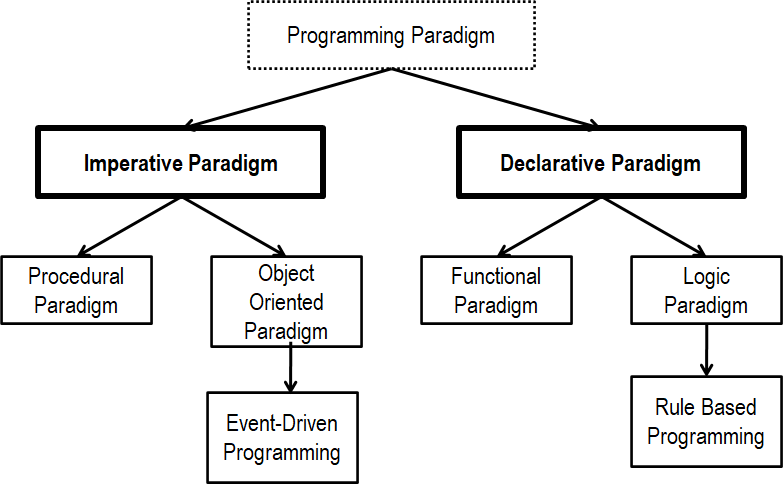
\includegraphics[width=0.75\textwidth]{../figures/paradimas_simao.png}
  \caption*{Fonte: Autoria própria}
  \label{fig:paradigmas_simao}
\end{figure}

\subsection{Paradigmas Imperativos}\label{sec:imperativos}

Nesta seção busca-se apresentar os paradigmas imperativos, ou subparadigmas
imperativos conforme o ponto de vista, mencionados na Seção
\ref{sec:paradigmas}, de modo a estabelecer a sua relação e características em
comum, assim como suas peculiaridades. Os subparadigmas que seguem os princípios
do Paradigma Imperativo (PI) se caracterizam pela flexibilidade de programação e
pela forma explicitamente sequencial pela qual as instruções são executadas
\cite{msc_Banaszewski_2009}. O Paradigma Procedimental (PP) foi o primeiro,
propriamente dito, paradigma de programação proposto, o qual faz parte do âmago
do PI. Posteriormente surge uma forma mais avançada de desenvolvimento em PI,
conhecida como Paradigma Orientado a Objetos (POO) \cite{msc_Banaszewski_2009}.
O PP e o POO se diferenciam pela forma como os elementos e instruções são
organizados, sendo o POO considerado mais rico e estruturado em termos de
abstração e expressão do código \cite{doc_ronszcka_2019}.

\subsubsection{Paradigma Procedimental (PP)}

O Paradigma Procedimental (PP) define um estilo de programação baseado na
organização sequencial de variáveis e comandos, na qual as variáveis representam
os estados das entidades e os comandos executam ações sobre estes estados
\cite{watt_2004,brookshear_2006}. O PP ainda vigora pelos motivos de
considerável coeficiente de modularização, certa simplicidade de programação em
sistemas de menor escala e relativa eficiência, uma vez que a forma de
codificação dos comandos condiz com a forma pela qual os mesmos são executados
pela máquina. Este fato facilita a geração de executáveis enxutos e eficientes
\cite{msc_Banaszewski_2009}. Outro fator que contribui para a permanência deste
paradigma é a experiência adquirida há anos pelos programadores neste tipo de
linguagem, o que é aqui chamado de inércia cognitiva. Neste sentido, alguns
exemplos clássicos de linguagens baseadas no PP são FORTRAN, COBOL, ALGOL,
BASIC, PASCAL e C \cite{msc_Banaszewski_2009}.

Como exemplo de programa no PP, o Código \ref{cod:alarm_c} apresenta um programa
que executa a lógica de tomada decisão sobre o estado de um dado uma aplicação
de sensor, cujo funcionamento já foi descrito na Seção \ref{sec:pon} sob a forma
de \textit{Rules}. Esse exemplo é também utilizado nas seções seguintes de forma a
ilustrar o uso dos diversos paradigmas. Esta implementação no PP é feita de
forma simples, na clássica linguagem de programação C, implementando o
\textit{Sensor} como uma \textit{struct} (estrutura) com duas variáveis membros, sendo
declaradas funções auxiliares para alterar os valores destas variáveis da
\textit{struct} utilizando ponteiros. Adicionalmente, a verificação dos estados
do \textit{Sensor} é feita por meio de um laço de repetição na função
\textit{main}.

\lstinputlisting[language=C++, float=htb, caption = {Exemplo de aplicação de
      sensor em C}, source = {Autoria própria}, label = {cod:alarm_c}]
{../code/ex_pp.cpp}

Em que pese suas vantagens, o PP apresenta certas deficiências, de tal forma que
subsequentemente e mais recentemente, o PP perdeu espaço considerável para o
POO. O PP é limitado no que diz respeito à sua capacidade de representar
abstrações, não possuindo ferramental que realmente induza à coesão de variáveis e
procedimentos diretamente relacionados, por exemplo. O PP só possui um único
mecanismo explícito de modularização, para favorecer a coesão, que é a divisão
do programa em rotinas. Neste sentido, novas ferramentas que aumentam a
capacidade de abstração do PP são introduzidas com o Paradigma Orientado a
Objetos (POO) \cite{Avacheva_2020}.

\subsubsection{Paradigma Orientado a Objetos (POO)}

O Paradigma Orientado a Objetos (POO) apresenta um nível de abstração mais alto
que o PP. Os programas desenvolvidos em POO são compostos por entidades
modulares denominadas objetos, que podem ser entendidas como abstrações de uma
entidade real ou imaginária, contendo as características pertinentes para sua implementação
computacional \cite{poo_2007}. Esses objetos agrupam atributos (similar às
variáveis do PP) e métodos (similar às funções do PP), organizados de maneira a
estimular coesão e desacoplamento, tudo à luz de seus tipos ou classes que ditam
o modelo de suas instâncias, incluindo os seus relacionamentos para com outros
objetos \cite{watt_2004,brookshear_2006,pressman_2016,msc_santos_2017}. Exemplos
de linguagens que materializam este paradigma são a SIMULA, Smalltalk, C++, JAVA
e C\# \cite{msc_Banaszewski_2009}.

Como exemplo do POO, no Código \ref{cod:alarm_cpp} é apresento um programa em
C++ que executa a lógica de tomada decisão sobre o estado de um dado uma
aplicação de sensor, cujo funcionamento é descrito na Seção \ref{sec:pon} sob a
forma de \textit{Rules}. Esse exemplo foi também apresentado anteriormente como
exemplo de implementação para o PP. A diferença entre a aplicação do POO e do PP
é justamente o encapsulamento da entidade \textit{Sensor}, agora implementada
por meio de uma classe com métodos próprios.

\lstinputlisting[language=C++, caption = {Exemplo de aplicação de sensor em
      C++}, source = {Autoria própria}, label = {cod:alarm_cpp}, float=htb]
{../code/ex_poo.cpp}

\subsubsection{Considerações Sobre os Paradigmas Imperativos}

Programas desenvolvidos com POO ou com o PP são concebidos como sequências de
instruções. Esse mecanismo de execução sequencial consiste em buscas, por assim
dizer, ou, mais precisamente, percorrimentos sobre entidades passivas (as
variáveis, os atributos e afins, vetores destes, estruturas de dados desses e
afins) que correspondem aos dados. Isto se dá por meio de comandos de decisão
(\textit{e.g.}, \textit{if-else} e \textit{switch} em linguagem C/C++), sendo
estes executados em laços de repetição (\textit{e.g.}, \textit{for},
\textit{while}, \textit{do-while} em linguagem C/C++) \cite{msc_santos_2017}.

Devido à sequencialidade da busca/percorrimentos e à passividade dos elementos
presente nas linguagens do PP e do POO, trechos de código tendem a se tornar
interdependentes, levando a acoplamentos, bem como há ainda correlatos problemas
de redundância na execução dos programas. Neste âmbito, as expressões causais
são avaliadas passivamente ocasionando as chamadas redundâncias temporais e
estruturais \cite{msc_Banaszewski_2009}. A redundância temporal, ocorre quando
há a reavaliação de expressões causais desnecessárias na presença de estados já
avaliados e inalterados, enquanto redundância estrutural ocorre quando o
conhecimento sobre um estado resultante da avaliação de uma expressão lógica não
é compartilhado entre outras expressões causais pertinentes em diferentes partes
do código, causando reavaliações desnecessárias. No pseudocódigo do Código
\ref{cod:loops} a redundância temporal é observada na linha 2, pelo laço de
repetição \textit{while(true)}, enquanto a redundância estrutural é
exemplificada nas linhas 3 e 12, nas quais o mesmo atributo \textit{attribue\_1}
do \textit{object\_1} é avaliado redundantemente nos dois \textit{ifs}. Estes
problemas podem afetar o desempenho dos programas desenvolvidos
\cite{msc_Banaszewski_2009}.

\begin{lstlisting}[numbers=left,
  stepnumber=1, caption = {Exemplo de
  redundâncias estruturais e temporais}, float=htb, source = {Autoria própria}, label =
  {cod:loops}]
...
while (true) do
    if ((object_1.attribute_1 == 1) and
        (object_1.attribute_2 == 1) and
        (object_1.attribute_3 == 1))
    then
        objetct_1.method_1();
        objetct_2.method_1();
        objetct_2.method_1();
    ...
    end_if
    if ((object_1.attribute_1 == 1) and
        (object_1.attribute_n == n) and
        (object_1.attribute_n == n))
    then
        objetct_1.method_n();
        objetct_2.method_n();
        objetct_2.method_n();
    ...
    end_if
end_while
...
\end{lstlisting}

\subsection{Paradigmas Declarativos}\label{sec:declarativos}

Da mesma forma como foi mostrado na Seção \ref{sec:imperativos} em relação aos
Paradigmas Imperativos, esta seção apresenta os Paradigmas Declarativos, de modo
a estabelecer a sua relação e características em comum assim como suas
peculiaridades. Os subparadigmas que seguem o PD, por sua vez seriam o Paradigma
Funcional (PF) e particularmente o Paradigma Lógico (PL), sabendo que, na verdade,
o PF estaria em uma fronteira com PI. 

Em todo caso, os subparadigmas PF e PL do PD caracterizam-se e diferenciam-se
dos subparadigmas do PI puro ao apresentar modelo menos flexível, porém mais
simplificado de programação. Mesmo no PF e certamente no PL, o programador se
concentraria mais na organização do conhecimento  em alto nível sobre a
resolução do problema computacional em si ao invés da implementação mais técnica
propriamente dita \cite{doc_ronszcka_2019}.

Enquanto o PI em geral impõe pesquisas orientadas a laços de repetições sobre
elementos passivos, relacionando dados a expressões causais, o PD possui
soluções declarativas que trabalham por recursões e/ou mecanismos de inferência.
Inclusive, alguns destes mecanismos no PL permitem evitar parte das redundâncias de
execução, conforme discutido no decorrer desta seção \cite{doc_ronszcka_2019}. 

%Dentre
%elas podem ser citados os Sistemas Baseados em Regras (SBRs), que tem como base
%algoritmos de inferência otimizados como o RETE \cite{forgy_1982}, o TREAT
%\cite{miranker_1987}, o LEAPS \cite{miranker_1990} e o HAL \cite{lee_2002}. Sem
%a aplicação destas soluções eficientes ciclos de inferência se tornariam muito
%lentos, inviabilizando a sua utilização em muitos casos \cite{doc_simao_2005}.

\subsubsection{Paradigma Funcional (PF)}

O Paradigma Funcional (PF) é baseado no conceito de funções computáveis por meio
do cálculo \textit{lambda}, que é um conceito que foi matematicamente
introduzido em 1936 por Alonzo Church \cite{henk_1984}. A essência do PF é a
construção de programas a partir da manipulação de dados por meio de funções, em
um modelo no qual as funções podem invocar outras funções ou até mesmo serem
passadas como parâmetros para outras funções
\cite{scott_2000,msc_Banaszewski_2009}. As funções do PF são ditas puras, no
sentido que seu resultado depende apenas da sua entrada, devido às funções não
possuírem estado compartilhado interno \cite{scott_2000}.

No Código \ref{cod:sensor_clj} o mesmo exemplo da aplicação de sensores é
apresentado, desta vez implementado no Paradigma Funcional por meio do uso da
linguagem Clojure, que é um dialeto dinâmico e funcional da linguagem de
programação Lisp.

Uma das vantagens desse paradigma é permitir a programação em mais alto nível
que o PP e POO puras justamente por permitir flexibilidades como a passagem de
funções como parâmetros. Além disso, o uso de funções puras facilita o
paralelismo, pois não existe estado compartilhado
\cite{scott_2000,bhadwal_2020}. Em contrapartida, a falta de estado
compartilhado combinado com recursão pode e tende a causar redução no desempenho
do programa \cite{bhadwal_2020}. Adicionalmente, ainda que o estilo de
programação funcional supostamente facilite escrever as funções, ele dificulta a
integração com outras áreas do código, principalmente operações de entrada e
saída de dados, como no caso interfaces e arquivos \cite{bhadwal_2020}.

\begin{lstlisting}[caption = {Exemplo de
aplicação de sensor em Clojure}, float=htb, source = {Autoria própria}, label =
{cod:sensor_clj}]
;; Autoria: Gustavo Brunholi Chierici - Data 22/06/2021 - Grupo de Pesquisa: PON - UTFPR

(defrecord FPSensor [is-read is-activated])     ;; Record ("struct") do sensor

(defn create-sensor [] (FPSensor. false false)) ;; Função que retorna um sensor

(defn activate-sensor                           ;; Função que "ativa" o sensor
    [sensor]
    (assoc sensor :is-activated true :is-read false))

(defn deactivate-sensor                         ;; Função que "desativa" o sensor
    [sensor]
    (assoc sensor :is-activated false))

(defn read-sensor                               ;; Função que "lê" o sensor
    [sensor]
    (assoc sensor :is-read true))

(defn check-sensor                              ;; Função que verifica se o sensor está ativado e o "lê" em caso positivo
    [sensor]
    (if (and (:is-activated sensor) (not (:is-read sensor)))
        (deactivate-sensor (read-sensor sensor)) sensor))
\end{lstlisting}

Alguns exemplos de linguagens baseadas no PF são LISP, Clojure, Miranda,
Haskell, Sisal, pH e ML \cite{msc_Banaszewski_2009}. Além destas linguagens,
C++11 em diante, C\# 3.0 e Java 8 também adicionaram construções que facilitam o
desenvolvimento de programas no estilo funcional, ainda que de forma híbrida e
dominada por seus paradigmas de origem \cite{bhadwal_2020}.

\subsubsection{Paradigma Lógico (PL)}

Apesar dos subparadigmas apresentados anteriormente (PP, POO e mesmo PF) se
basearem em teorias diferentes, eles acabam compartilhando a mesma forma de
execução em alguma medida. Mais precisamente, em todos eles, um programa ou
mesmo uma função, recebe dados como entrada, realiza computações e gera uma
saída via um mapeamento direto interno. Este processo é definido como um
mapeamento da entrada para a saída do programa
\cite{watt_2004,msc_Banaszewski_2009}.

No PL, além das entidades com suas variáveis e comandos usuais (\textit{i.e.},
base de fatos) em formas como frames (aparentados de objetos, mas com métodos
suspostamente simples ou pragmáticos), os comandos lógicos causais também são
representados na forma de dados, sob o viés de regras (\textit{i.e.}, base de
regras) conforme Figura \ref{fig:rule_pl}. Não raro, linguagens e ambientes do
PL são chamados Sistemas Baseados em Regras (SBRs) justamente. Em todo caso,
essa relação entre base de fatos e base de regras, buscando aprovar/desaprovas
regras pelas suas confrontações, dá-se pela busca realizada por meio de algum
mecanismo de inferência sobre as definições de elementos factuais (e.g., frames)
da base de fatos vis-à-vis expressões causais (normalmente regras) da base de
regras, conforme Figura \ref{fig:fact_base} \cite{msc_Banaszewski_2009}. Isto
dito, alguns exemplos de linguagens que implementam o PL são  Oz
\cite{van_roy_2004}, Prolog, RuleWorks e OPS \cite{msc_Banaszewski_2009}.

\begin{figure}[!htb]
\centering\caption{Conhecimento representado em regras no PL}
\smallskip
\subcaptionbox{Entidades}{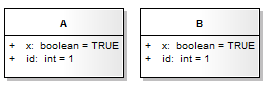
\includegraphics[width=0.50\textwidth]{../figures/ab_pl.png}}%
\hfill
\subcaptionbox{Regra}{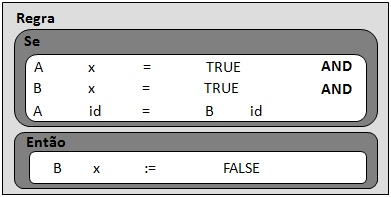
\includegraphics[width=0.50\textwidth]{../figures/rule_pl.png}}%
\caption*{Fonte: \citeonline{msc_Banaszewski_2009}}
\label{fig:rule_pl}
\end{figure}

\FloatBarrier

Ainda, há linguagens do PL, como OPS e Ilog Rules, que tem como base algoritmos
de inferência otimizados como o RETE \cite{forgy_1982}. Outros exemplos de
algoritmos de inferência otimizados são TREAT \cite{miranker_1987} e o LEAPS
\cite{miranker_1990} derivados do RETE, bem como o alternativo o HAL
\cite{lee_2002}. Sem a aplicação destas soluções eficientes ciclos de inferência
se tornariam muito lentos, inviabilizando a sua utilização em muitos casos.
Entretanto, mesmo com algoritmos de inferência considerados eficientes, ainda há
redundância de processamentos e preço de representar base de fatos e base de
regras em estrutura de dados \cite{doc_simao_2005,msc_Banaszewski_2009}.

\begin{figure}[!htb]
  \centering
  \caption{Arquitetura interna de um Sistema Baseado em Regras}
  \smallskip
  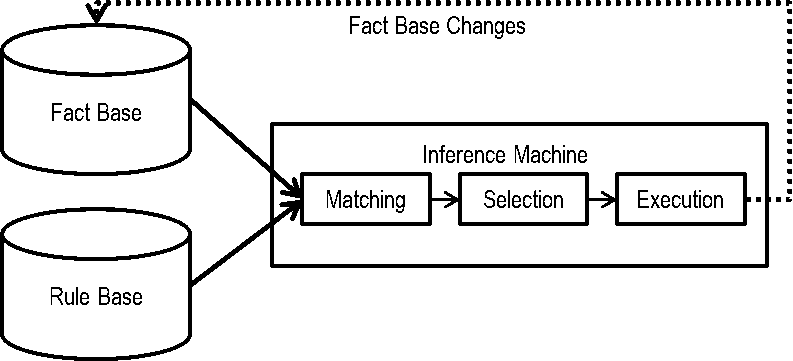
\includegraphics[width=0.6\textwidth]{../figures/fact_base.png}\smallskip
  \caption*{Fonte: \citeonline{msc_Banaszewski_2009}}
  \label{fig:fact_base}
\end{figure}

O RETE em particular implementa um processo de busca otimizado, manipulando
elementos da base de fatos e regras sobre uma estrutura baseada em redes ou
grafos. Esse processo é ilustrado de forma simplificada na Figura
\ref{fig:rete}. Mais precisamente, o RETE guarda informação sobre avaliações
anteriores das regras e também avalia as regras somente quando a base de fatos é
atualizada de modo a evitar avaliações redundantes, ou seja, quando um elemento
da base de fatos é inserido/modificado/removido da Base de Fatos. Com isto, o
RETE resolve o problema das redundâncias temporais do PI. Esta solução se faz
possível porque o RETE é composto de duas sub-redes: a $\alpha$-network é composta
por nós sendo cada qual responsável pela avaliação lógica de fatos; a
$\beta$-network, por sua vez, é composta por outros nós, sendo cada qual
responsável pela correlação entre fatos. Se as avaliações e correlações forem
satisfeitas para uma regra, a mesma é aprovada sendo, portanto, inserida no
conjunto de conflito
\cite{forgy_1982,doorenbos_1995,msc_Banaszewski_2009}

\begin{figure}[!htb]
  \centering
  \caption{Estrutura do algoritmo RETE}
  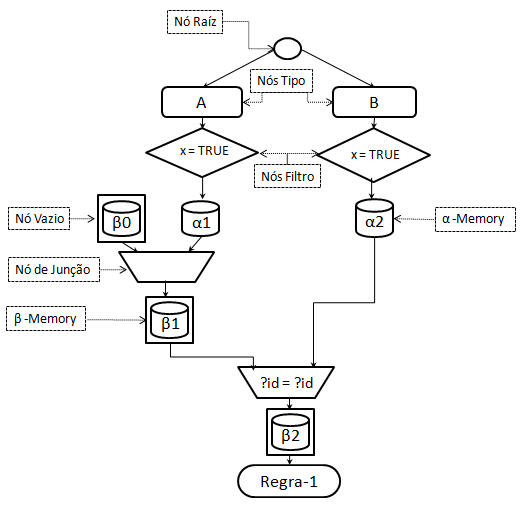
\includegraphics[width=0.65\textwidth]{../figures/inference_machine.png}
  \caption*{Fonte: \citeonline{msc_Banaszewski_2009}}
  \label{fig:rete}
\end{figure}

No Código \ref{cod:sensor_ruleworks} novamente o exemplo da aplicação de tomada de
decisão sobre um sensor é apresentado, desta vez implementado no Paradigma
Lógico com a linguagem de programação RuleWorks. Observa-se que, por se tratar
de uma linguagem de programação cuja estrutura se baseia em regras, o código tem
apresenta muita similaridade ao representado sob a forma de \textit{Rule} na
Figura \ref{fig:nop_rule}.

\begin{lstlisting}[
  caption = {Exemplo de aplicação de sensor em RuleWorks},
  float=htb,
  source = {Autoria própria},
  label = {cod:sensor_ruleworks}
]
(object-class sensor
    ^is-read
    ^is-activated
)

(rule process-sensor:sensor
    (sensor ^$ID <the-sensor> ^is-read <false> ^is_activated <true>)
    -->
    (bind <the-sensor ^is-read> (false))
    (bind <the-sensor ^is-activated>  (false))
)
\end{lstlisting}

\subsubsection{Considerações Sobre os Paradigmas Declarativos}

O PD se propõe a resolver algumas das deficiências do PI, principalmente aquelas
relacionadas à dificuldade de programação em ambientes \textit{multicore},
atualmente no caso do PL contemporâneo, e redundâncias estruturais e temporais,
no caso do PL/SBR com máquinas de inferência apropriadas. Apesar disso, a
maioria destas deficiências ainda se repete devido aos mecanismos de execução
tanto do PF como do PL que se baseiam em buscas sob elementos passivos, que por
sua vez ou reproduzem estes mesmos problemas de redundâncias estruturais e
temporais e/ou os atenuam com algoritmos inferência dito otimizados, mas trocando
os problemas por estruturas de dados caras. Assim, normalmente programas em PD
são mais lentos que em PI, apesar das redundâncias deste
\cite{msc_Banaszewski_2009}.

Além disso, enquanto as linguagens de programação do PD apresentam um modelo de
programação mais simplificado, elas também não oferecem a mesma flexibilidade
das linguagens do PI. Isto pode dificultar a construção de códigos mais
eficientes, visto que limita o controle que o programador tem sobre o
\textit{software}. Finalmente, mesmo no caso de PF, tanto em PD quanto PI em
geral, a orientação a buscas e/ou percorrimentos deles não permite alcançar
facilmente módulos desacoplados, particularmente em nível granular, o que
dificulta processamentos paralelo e/ou distribuídos \cite{msc_Banaszewski_2009}.

\subsection{Paradigmas Emergentes}

Em suma, como já dito, os paradigmas dominantes PI (com PP e POO) e PD (com PF e
PL) tendem a ter problemas similares de redundâncias e/ou processamentos e
acoplamentos. Isto dificulta alcançar demandas contemporâneas como a facilitação
de programação em alto nível, boa performance de processamento e boa performance
do paralelismo/distribuição de processamento em arquiteturas com múltiplos
núcleos, por exemplo. 

Outrossim, além dos paradigmas dominantes, há os paradigmas emergentes que não
raro se materializam sobre os dominantes. Muito embora emergentes conhecidos não
tenham resolvidos esses problemas relatados dos dominantes, eles sim trazem
novas conotações de desenvolvimento. Exemplos de paradigmas emergentes (talvez
mais conhecidos) são como Paradigma Orientado a Componentes (POC), Paradigma
Orientado a Eventos (POE), Paradigma Orientado a Aspectos (POA), Paradigma
Orientado a Agentes (POAg) e Paradigma Orientado a Atores (POAt).


\subsubsection{Paradigma Orientado a Componentes (POC)}

O Paradigma Orientado a Componentes (POC) se baseia no reuso e combinação de
componentes. Um componente consiste em uma parte do programa desenvolvida de
forma a ser altamente reutilizável, que pode ser desenvolvida independentemente
para ser depois combinada com outras partes objetivando construir uma unidade
maior \cite{dsouza_1998}.

Na Figura \ref{fig:componentes} um diagrama de componentes é exemplificado, no
qual os componentes se relacionam para realizar o fluxo de execução do programa.
As setas direcionais representam a invocação de serviços oferecidos por estes
componentes. Os serviços não são acessados diretamente, mas por meio de
entidades descritoras, chamadas de interfaces. O uso de interfaces é uma
característica do POC que permite que a definição dos serviços seja feita
completamente separada da implementação \cite{crnkovic_2002}

\begin{figure}[!htb]
  \centering
  \caption{Diagrama de componentes}
  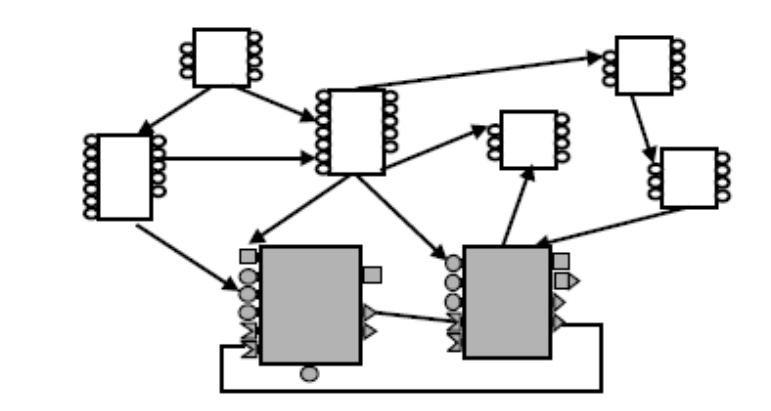
\includegraphics[width=0.8\textwidth]{../figures/componentes.png}
  \caption*{Fonte: \citeonline{crnkovic_2002}}
  \label{fig:componentes}
\end{figure}

O POC é muito utilizado em \textit{frameworks} de programação de
\textit{front-end}, como React\footnote{Para maiores detalhes sobre este
\textit{framework}, consultar \url{https://reactjs.org/}}, Angular\footnote{Para
maiores detalhes sobre este \textit{framework}, consultar
\url{https://angular.io/}} e VUE\footnote{Para maiores detalhes sobre este
\textit{framework}, consultar \url{https://vuejs.org/}}. No Código
\ref{cod:components_js}, é mostrado o exemplo de tomada de decisão sobre um
sensor em linguagem de programação JavaScript com o \textit{framework} Angular,
na qual pode ser observado que a implementação do sensor importa e implementa a
funcionalidade do componente \textit{OnInit}.

A principal desvantagem do POC é que o foco na reusabilidade dos componentes
tende a aumentar a complexidade deles, de modo que se torna necessário a
execução de processos mais cuidadosos de planejamento do sistema e manutenção
dos componentes. Quanto mais reutilizável for o componente, mais complexo ele se
torna e mais difícil é a sua manutenção \cite{crnkovic_2002}. Por fim,
internamente o POC é, na prática, o encapsulamento de módulos criados via
paradigmas já existentes.

\begin{lstlisting}[caption = {Exemplo de aplicação de sensor em React no POC},
  source = {Autoria própria}, float=htb,
  label  = {cod:components_js}]
  /* Autoria: Prof. Dr. Roni Fabio Banaszewski - Data 24/06/2021 - Grupo de Pesquisa: PON - UTFPR */ 
  
  import {Component, OnInit} from '@angular/core';
  import {BehaviorSubject} from "rxjs";
  
  @Component({
    selector: 'app-root',
    templateUrl: './app.component.html',
    styleUrls: ['./app.component.css']
  })
  
  export class AppComponent implements OnInit {
    title = 'sensor-app';
  
    ready: boolean = false;
    active: boolean = true;
  
    private readySubject = new BehaviorSubject<boolean>(this.ready);
    private activeSubject = new BehaviorSubject<boolean>(this.active);
  
    ngOnInit() {
      this.readySubject.subscribe(value => {
        this.ready = value;
        this.rule()
      });
  
      this.activeSubject.subscribe(value => {
        this.active = value;
        this.rule()
      });
    }
  
    rule() {
      if (this.ready == false && this.active == true) {
        this.readySubject.next(true);
        this.activeSubject.next(false);
      }
    }
  }
\end{lstlisting}

\subsubsection{Paradigma Orientado a Eventos (POE)}\label{sec:poe}

No Paradigma Orientado a Eventos (POE) as entidades interagem por meio da
ocorrência de eventos. Um evento consiste em uma condição detectável que pode
instigar a execução de um método. O objeto capaz de detectar a condição e gerar
o evento é chamado de objeto transmissor, enquanto os objetos interessados que
recebem um evento são chamados de objetos receptores \cite{ferg_2006}.

A Figura \ref{fig:eventos} ilustra a relação entre os objetos transmissores e
receptores, que podem ocorrer de forma direta ou indireta. No exemplo à esquerda
na Figura \ref{fig:eventos}, um objeto transmissor detecta a ocorrência de um
evento e notifica este evento diretamente aos objetos receptores interessados.
No exemplo à direita na Figura \ref{fig:eventos}, o evento é transmitido por
intermédio do objeto \textit{Dispatcher} \cite{msc_xavier_2014}. A transmissão
do evento ocorre por meio da passagem de um \textit{token}, o qual pode ser
representado por uma mensagem formada por uma cadeia de caracteres ou um objeto
com dados \cite{ferg_2006}.

\begin{figure}[!htb]
  \centering
  \caption{Processo de detecção de eventos}
  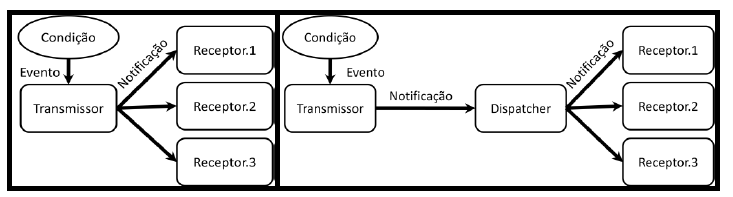
\includegraphics[width=\textwidth]{../figures/eventos.png}
  \caption*{Fonte: \citeonline{faison_2006}}
  \label{fig:eventos}
\end{figure}
\FloatBarrier

Na verdade, não existe linguagem de programação que implementa especificamente o
POE, sendo ele incorporado por \textit{frameworks} e afins nas linguagens dos
paradigmas vigentes. Por exemplo, um \textit{framework} muito popular para C++ e
Python que implementa a orientação a eventos é o Qt\footnote{Para maiores
  detalhes sobre este \textit{framework}, consultar \url{https://www.qt.io/}}. Em
suma, o Qt é um \textit{framework} para a criação de aplicações gráficas de
forma intuitiva, usando técnica para tal conhecida como \textit{Rapid
  Application Development} (RAD). Neste \textit{framework}, um caso muito comum
para o uso de eventos é mostrado no Código \ref{cod:qt_event}, no qual os
eventos são enviados para ativar o sensor ao pressionar um botão, ao conectar o
evento \textit{button.clicked} às funções \textit{Activate()} e
\textit{Process()}.

\begin{lstlisting}[language = Python, float=htb,
  caption = {Exemplo de aplicação de sensor com PyQt5 no POE},
  source = {Autoria própria},
  label = {cod:qt_event}]
class Sensor(QWidget):
    isRead = False
    isActivated = False
    button = QPushButton('Activate')
    
    def Activate(self):
        self.isActivated = True
        self.isRead = False    
    def Deactivate(self):
        self.isActivated = False
        self.isRead = False          
    def Process(self):
        if(self.isActivated and not self.isRead):
            alert = QMessageBox(self)
            alert.setText('Sensor Processed')
            alert.show()
            self.Deactivate()    
    def __init__(self):
        super().__init__()
        self.button.clicked.connect(self.Activate)
        self.button.clicked.connect(self.Process)
        self.button.show()
\end{lstlisting}

Dentre os Paradigmas Emergentes mencionados na Seção \ref{sec:intro_emergentes},
o POE se destaca pelo seu estado de maturidade e extenso uso em diversas
aplicações, desta forma podendo ser considerado um paradigma em fase de
transição de Paradigma Emergente para Paradigma Dominante. Dentre as vantagens
do POE estão a flexibilidade e simplicidade de programação devido ao mecanismo
de eventos, que facilita a interação entre entidades no código, como o botão
\textit{Activate} com o sensor do exemplo. Em contrapartida, o código pode ser
considerado confuso, devido ao fluxo de execução do programa, o que também
dificulta encontrar erros no programa quando comparado a paradigmas com fluxo de
execução mais simples como o do PI ou com lógica em bases de conhecimento
unívocas como em SBR/PL do PD. 

\subsubsection{Paradigma Orientado a Aspectos (POAs)}

O Paradigma Orientado a Aspectos (POAs) permite separar as funcionalidades
principais de funcionalidades secundárias de um código típico orientado a
objetos, encapsulando as funcionalidades secundárias em uma unidade modular
chamada de aspecto. No contexto do POA, a funcionalidade principal é uma
funcionalidade única implementada por determinada função ou método, enquanto as
funcionalidades secundárias são genéricas e compartilhadas entre várias funções
ou métodos \cite{laddad_2003}.

O POAs propõe essa separação por meio do encapsulamento das funcionalidades
secundárias, sob a forma de aspectos, para serem invocadas implicitamente (sem a
declaração da chamada dos métodos explicitamente no código) pelas
funcionalidades principais. Os aspectos são invocados pela chamada dos métodos
que implementam as funcionalidades principais \cite{miles_2004}. A vantagem da
aplicação desse mecanismo seria maior incentivo ao reuso de código e maior
facilidade de entendimento ou alteração do código
\cite{miles_2004}.

Um exemplo de linguagem de programação na qual pode ser realizada a aplicação do
POA é Python, que conta com suporte nativo da linguagem ao POA por meio dos
chamados \textit{decorators}. No exemplo do Código \ref{cod:python_aspect}, no
qual é implementado o exemplo da aplicação de sensor, essa ferramenta é
utilizada para encapsular a verificação dos estados dos atributos do sensor por
meio do aspecto \textit{checker\_aspect}.

\begin{lstlisting}[
language = Python, %float=htb,
  caption = {Exemplo de aplicação de sensor em Python no POAs},
source = {Autoria própria}, float=htb,
label = {cod:python_aspect}]
# Autoria: Marcos Talau e Felipe Neves - Data 26/06/2021 - Grupo de Pesquisa: PON - UTFPR 
def checker_aspect(func):
    def wrapper(self):
        func(self)
        if(self.isActivated and not self.isRead):
            self.Process()
    return wrapper

class Sensor:
    isRead = False
    isActivated = False

    @checker_aspect
    def Activate(self):
        self.isActivated = True
        self.isRead = False
    @checker_aspect
    def Deactivate(self):
        self.isActivated = False
        self.isRead = False
    def Process(self):
        self.Deactivate()
\end{lstlisting}

%TODO: desvantagens POAs

\subsubsection{Paradigma Orientado a Agentes (POAg) / Atores (POAt)}

O Paradigma Orientado a Agentes (POAg) permite construir programas empregando
entidades chamadas agentes. Os agentes são entidades computacionais capazes de
executar ações de maneira flexível e autônoma, de modo a atingir objetivos
estabelecidos no momento da sua concepção \cite{jennings_1999}.

Os agentes são usualmente implementados sobre os conceitos do POO, porém agentes
possuem propriedades mais complexas do que um objeto. Diferente dos objetos, que
atuam passivamente até que um de seus métodos sejam invocados, agentes podem
atuar de forma proativa, tendo objetivos individuais ou coletivos. Um objeto
aguarda até que seja lhe indicado o que fazer, enquanto o agente decide por si
só quando e o que deve ser feito. Ainda, em POAg as relações entre os entes
acontecem na dinâmica do sistema, de maneira fluida e não tudo pré-definido como
normalmente ocorre em POO \cite{msc_Banaszewski_2009}.

No Código \ref{cod:agent_ex}, é mostrado o exemplo de tomada de decisão sobre um
sensorem linguagem de programação Elixir/Erlang. Neste exemplo simples, pode ser
observada a complexidade presente devido às funcionalidades básicas necessárias
para a comunicação entre agentes.

O Paradigma Orientado a Atores (POAt) é consideravelmente similar ao POAg, sendo
o modelo de agentes uma extensão do modelo de atores. A diferença entre agentes
e atores é que os agentes são tipicamente mais complexos e capazes de tomada de
decisão lógica \cite{cardoso_2013}. As principais linguagens do POAt são Akka e
Erlang. Ambos os modelos do POAt e POAg trazem a vantagem de facilitar o
paralelismo devido ao alto desacoplamento entre as entidades, enquanto uma das
principais desvantagens é o alto tempo de execução da comunicação entre os
atores/agentes.

\begin{lstlisting}[caption = {Exemplo de aplicação de sensor em Elixir no POAg}, %float=htb,
source = {Autoria própria}, language=elixir, float=htb,
  label = {cod:agent_ex}]
# Autoria: Fabio Negrini - Data 11/08/2021 - Grupo de Pesquisa: PON - UTFPR
defmodule Sensor do use GenServer
  def create() do
    state = init_state()
    {:ok, pid} = GenServer.start_link(__MODULE__, state, name: __MODULE__)
    pid
  end
  defp init_state() do
    %{:is_read   => false,
      :is_activated => false}
  end
  @impl true
  def init(stack) do
    {:ok, stack}
  end
  @impl true
  def handle_call(:is_read, _from, state) do
    is_read = Map.get(state, :is_read)
    {:reply, is_read, state}
  end
  def handle_call(:is_activated, _from, state) do
    is_activated = Map.get(state, :is_activated)
    {:reply, is_activated, state}
  end
  @impl true
  def handle_cast(:activate, state) do
    state = Map.put(state, :is_read, false)
    state = Map.put(state, :is_activated, true)
    {:noreply, state}
  end
  def handle_cast(:read, state) do
    state = Map.put(state, :is_read, true)
    {:noreply, state}
  end
  def handle_cast(:deactivate, state) do
    state = Map.put(state, :is_activated, true)
    {:noreply, state}
  end
end
\end{lstlisting}

\subsection{Considerações Sobre os Paradigmas Dominantes e Emergentes}

Esta seção permitiu contextualizar as principais características, como vantagens
e desvantagens dos paradigmas de programação atuais, tanto dos dominantes como
dos emergentes. Na Seção \ref{sec:motiv} foram levantadas as principais demandas
do desenvolvimento de \textit{software} atuais, que seriam a programação em alto
nível, paralelismo e desempenho. Nesse sentido, nenhum dos Paradigmas Dominantes
atende de forma simultânea a todas essas demandas. Conforme detalhado no Quadro
\ref{tab:demandas2}, o PI apesar de apresentar bom desempenho, não possibilita a
programação em alto nível e dificulta a implementação de paralelismo, enquanto o
PD apresenta tais características, porém o faz em troca de desempenho inferior
quando comparado ao PI.

\begin{table}[!htb]
  \centering
  \caption{Demandas de desenvolvimento de \textit{software} atendidas pelos
    Paradigmas Dominantes}
  \smallskip
  \begin{tabularx}{\textwidth}{|l||*{6}{X|}}\hline
    \diagbox{Demanda}{Paradigma} & Imperativo    & Declarativo    \\\hline\hline
    Programação em alto nível             &            & \checkmark \\ \hline
    Paralelismo                           &            & \checkmark \\ \hline
    Desempenho                            & \checkmark &            \\ \hline
  \end{tabularx}
  \caption*{Fonte: Autoria própria}
  \label{tab:demandas2}
\end{table}

\FloatBarrier

De todo modo os Paradigmas Emergentes mencionados também não por herdarem muitas
das defíciencias dos Paradigmas Dominantes. Isto é dado por muitos desses
paradigmas serem construídos com base nos Paradigmas Dominantes, ou
implementados nas linguagens de programação já existentes dos mesmos.
Feita esta revisão geral nesta seção, a seção seguinte enfim apresenta em
maiores detalhes o Paradigma Orientado Notificações (PON).

\pagebreak

\section{Paradigma Orientado Notificações (PON)}\label{sec:estado_arte_pon}

O Paradigma Orientado a Notificações (PON) é uma solução de desenvolvimento de
software que permite, entre outras características, excelente desempenho
computacional via entidades enxutas que colaboram por notificações precisas. O
inovador PON apresenta propriedades que unem a flexibilidade de programação do
Paradigma Imperativo (PI) e a facilidade de programação do Paradigma Declarativo
(PD) \cite{doc_ronszcka_2019,oshiro_2021}. 

Em suma e mais precisamente, o PON proporciona uma nova visão de desenvolver,
estruturar e executar software por meio de entidades facto-execucionais e
lógico-causais que colaboram por notificações precisas e pontuais [Ronszcka
2019]. Com isto, o PON apresenta três propriedades elementares, que consistem
em: (a) facilidade de programação orientada a regras em alto nível, (b) evitar
redundâncias de código lógico-causal que viabiliza alto desempenho de execução e
(c) desacoplamento implícito de construtos que viabiliza paralelismo e
distribuição \cite{doc_ronszcka_2019,oshiro_2021}.

De modo geral, dito de outra forma, o PON resolve certos problemas existentes
nos outros paradigmas de programação atuais (como PI e PD com seus subparadigmas
dominantes ou emergentes), os quais foram pragmaticamente revisados na Seção
\ref{sec:paradigmas} e detalhadamente revisados na literatura pertinente, como
em \citeonline{van_roy_2004,scott_2009,msc_Banaszewski_2009,msc_xavier_2014} e
\citeonline{doc_ronszcka_2019}. Exemplos de problemas dos paradigmas de
programação vigentes são enfim as redundâncias temporais e estruturais na
análise lógico-causal com o consequente mau uso do tempo de processamento, assim
como o acoplamento excessivo entre entidades computacionais que dificulta o
reaproveitamento e paralelização/distribuição das mesmas
\cite{pat_simao_2008,msc_Banaszewski_2009,doc_linhares_2015,msc_pordeus_2017,doc_Kerschbaumer_2018,doc_ronszcka_2019}.

\subsection{Constituintes do PON}

Muito embora o PON já tenha sido apresentado na introdução desta dissertação,
ele é aqui reapresentado de forma objetiva para facilitar o encadeamento da
leitura, bem como para fins de revisão. Substancialmente, o PON é constituído
por dois conjuntos de entidades computacionais: o facto-execucional e o
lógico-causal \cite{doc_ronszcka_2019,oshiro_2021}. A relação entre eles e as
entidades constituintes do PON, são ilustradas, no contexto de um sistema de
correlação de sensores, pela Figura \ref{fig:oshiro_pon}.

Conforme a Figura \ref{fig:oshiro_pon}, há entidades facto-execucionais
notificantes, os Fact Base Elements (FBE), que representam entidades do mundo e
são compostas de sub-entidades Attributes e sub-entidades Methods, as quais
respectivamente retratam seus estados e seus serviços/comportamento. Há também
entidades lógico-causais notificáveis, as Rules, sendo cada qual composta de uma
sub-entidade Condition e uma sub-entidade Action, que respectivamente se
associam à sub-entidades Premises e à sub-entidades Instigations. Em tempo de
construção das entidades, à luz de suas relações, são estabelecidos conexões
para fins de notificações entre elas \cite{doc_ronszcka_2019,oshiro_2021}. Em
suma, o ciclo de notificações funciona assim: cada Attribute de uma instância de
um FBE que mudar de estado notifica apenas as Premises efetivamente pertinentes,
o que faz com que essas refaçam seus cálculos lógicos. Cada Premise que mudar de
estado lógico notifica apenas as Conditions efetivamente pertinentes, fazendo
com que essas refaçam seus cálculos lógicos pelos estados notificados
contabilizados. Por sua vez, se a Condition for aprovada, ela pode aprovar sua
respectiva Rule. Esta, quando aprovada, ativa então sua Action, que notifica
suas Instigations. Estas enfim instigam precisamente os Methods. Estes últimos
geralmente alteram os estados dos Attributes, reativando o fluxo de notificações
\cite{doc_ronszcka_2019,oshiro_2021}.

\begin{figure}[!htb]
  \centering
  \caption{Interação entre as entidades do PON e ciclo de notificações}
  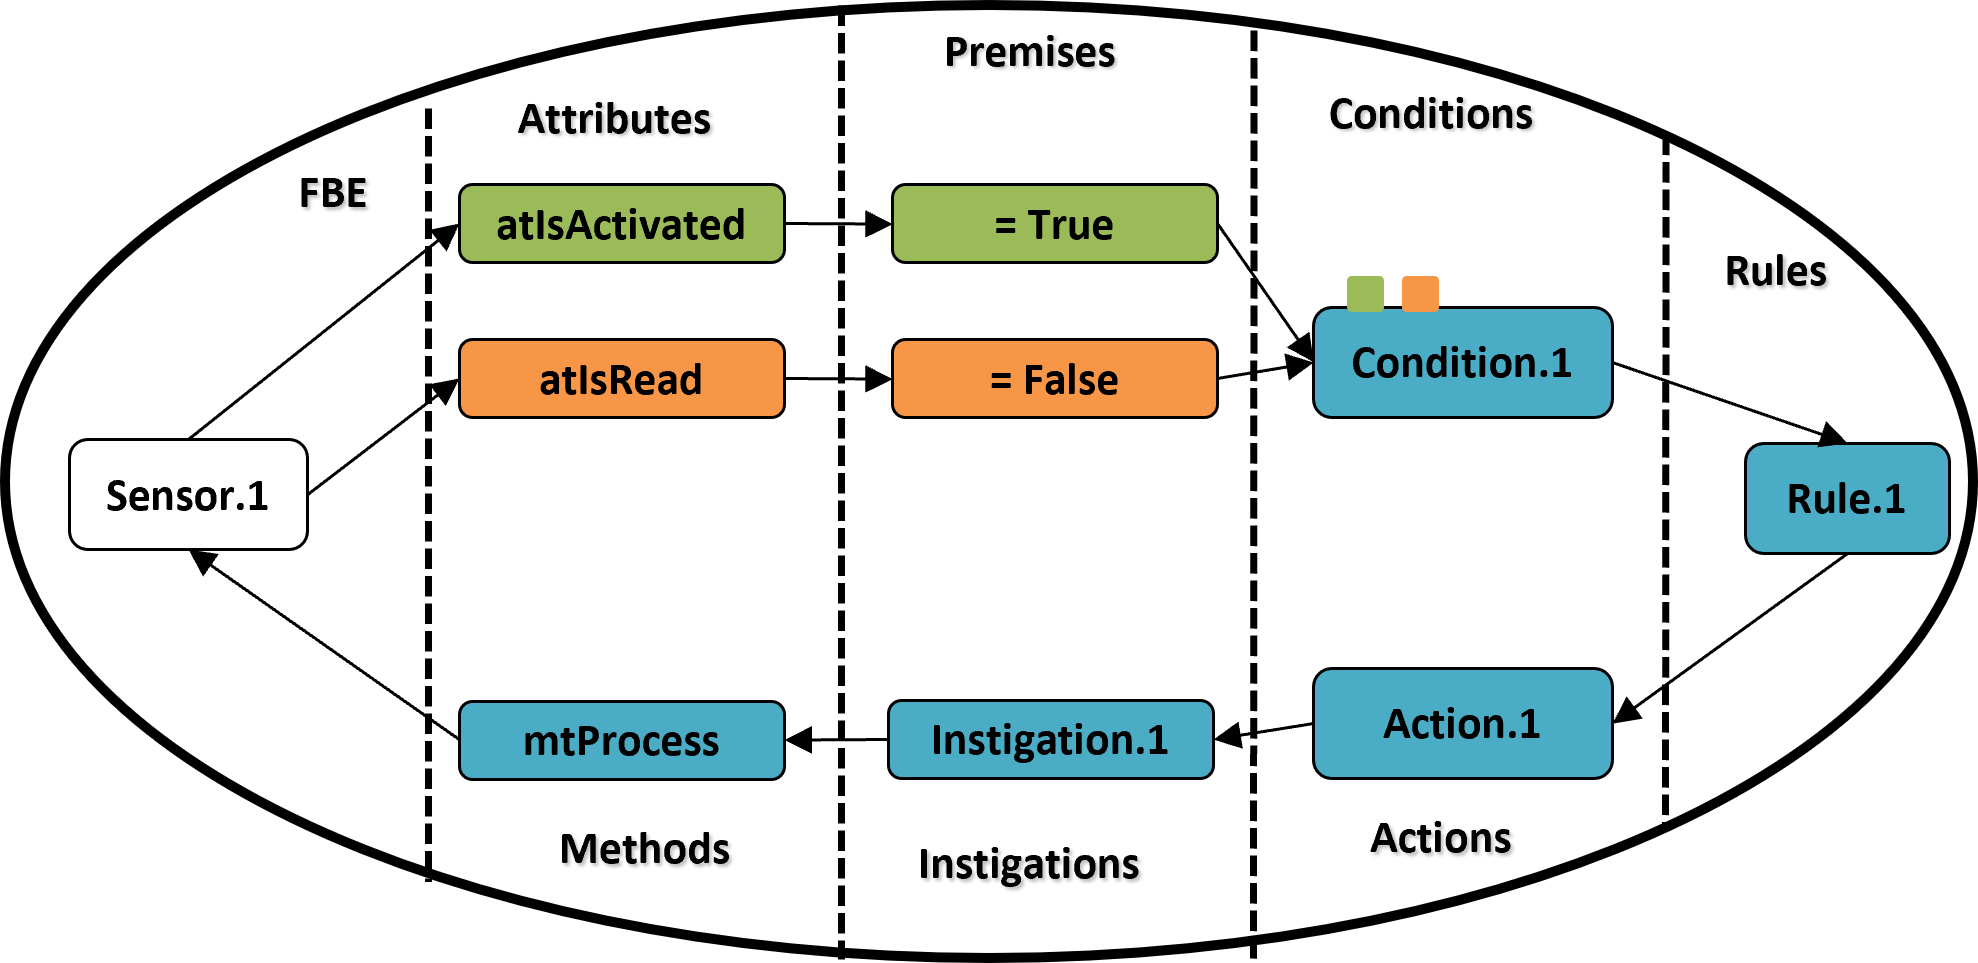
\includegraphics[width=0.9\textwidth]{../figures/nop_cycle.png}
  \smallskip
  \caption*{Fonte: Autoria Própria}
  \label{fig:oshiro_pon}
\end{figure}

Isto dito, o PON permite o desacoplamento das expressões lógico-causais do resto
do programa, por meio da aplicação destas entidades reativas e notificantes
justamente. Como as entidades apenas trocam notificações, elas não estão
fortemente acopladas entre si, o que é usualmente chamado de desacoplamento.
Essa característica favorece o desenvolvimento de aplicações paralelas e
distribuídas, ao mesmo tempo que mantém o desempenho das aplicações. Isso difere
do modelo de desenvolvimento usual, como no POO do PI e nos SBR do PD, nos quais
as expressões causais são passivas e acopladas a outras partes do programa,
conforme anteriormente elucidado
\cite{pat_simao_2008,simao_2009,msc_Banaszewski_2009,simao_2012a,doc_ronszcka_2019}.

No PON, a entidade reativa que trata a expressão causal é a \textit{Rule},
conforme acima explicado. Assim, cada \textit{Rule} gerencia o conhecimento
sobre o comportamento lógico-causal de um conjunto de \textit{FBEs} que a fazem
reagir pela cadeia de notificação de seus constituintes. Ainda, o conhecimento
lógico-causal de uma \textit{Rule} provém normalmente de uma regra se-então, o
que é uma maneira natural de expressão deste tipo de conhecimento, enquanto o
conhecimento facto-execucional dos FBEs provém em uma forma de expressão
compatível, similar a objetos ou \textit{frames} \cite{doc_ronszcka_2019}.

Uma vez que estas entidades Rules e FBEs são criadas à luz desses conhecimentos
lógico-causais e facto-execucionais, a cadeia de notificações também é
criada/conectada na criação das suas entidades constituintes. Essas entidades
computacionais notificantes precisamente que possibilitam que o mecanismo de
execução ocorra de forma reativa e naturalmente desacoplada, bem como
possibilitam a redução de redundâncias temporais e estruturais, viabilizando
inclusive boa performance e o paralelismo e/ou distribuição fina de
processamento \cite{simao_2012a}. A boa performance, particularmente,
encontraria lastro no cálculo assintótico da complexidade temporal dessas
entidades reativado PON, o que é abordado na seção seguinte.

\subsection{Complexidade temporal}\label{sec:complexidade}

Com base nas entidades reativas e notificantes do PON é possível calcular a
complexidade temporal da execução do mecanismo de notificações.
\citeonline{msc_Banaszewski_2009} define a complexidade assintótica para o pior
caso representada por O(n³) ou O(\textit{FactBaseSize} * \textit{nPremises} *
\textit{nRules}), onde \textit{FactBaseSize} corresponde ao número máximo de
objetos \textit{Attributes}, nPremises corresponde ao número máximo de entidades
\textit{Premises} notificadas por estes \textit{Attributes} e \textit{nRules}
corresponde ao número máximo de entidades \textit{Conditions-Rules} notificadas
por estas \textit{Premises} \cite{doc_simao_2005,msc_Banaszewski_2009}.

Esse cálculo é ilustrado na Figura \ref{fig:calculo_pon}, na qual
\textit{Attributes}, \textit{Premises}, \textit{Conditions} e \textit{Rules}
correspondem respectivamente aos símbolos com abreviações Att, Pr, Cd e Rl.
O caso assintótico considera o pior caso, no qual a alteração do estado do
\textit{Attribute} causa alteração no estado de todas as \textit{Premises}, que
por sua vez notificam todas as \textit{Conditions}, que também notificam todas
as \textit{Rules}. Entretanto, em um caso típico, a alteração do estado de um
\textit{Attribute} nem sempre causa alteração no estado de qualquer
\textit{Premise} ou \textit{Condition}, de forma que não são geradas tantas
notificações, permitindo um melhor desempenho do que o considerado no cálculo
assintótico.

Entretanto, ao invés de se considerar apenas o pior caso, pode ser analisada a
complexidade do caso médio. Neste caso, a análise da complexidade é iniciada no
começo do processo de notificação do PON, a partir da entidade
\textit{Attribute}. Desta forma, as principais variáveis envolvidas na
notificação de um \textit{Attribute} seriam $FBat() = nPremises * nRules$. A
variável \textit{nPremises} é a soma do número de entidades \textit{Premises} a
serem notificadas por dado \textit{Attribute} e a variável \textit{nRules} é a
soma do número de entidades \textit{Rules} dependentes da mudança de estado de
\textit{Premises} consideradas em \textit{nPremises}. Portanto, se for
considerado um ciclo de notificações como a notificação gerada por de um único
\textit{Attribute} e $n$ como sendo o número de total de \textit{Attributes} do
sistema, a complexidade temporal pode ser definida como $(FBat_{1}()+ ... +
FB_{n}()) / n$. Assim, o resultado desta média seria uma constante, o que
implicaria em uma complexidade linear $O(n)$ para o PON
\cite{doc_simao_2005,msc_Ronszcka_2012,doc_ronszcka_2019}.

\begin{figure}[!htb]
  \centering
  \caption{Cálculo assintótico do mecanismo de notificações}
  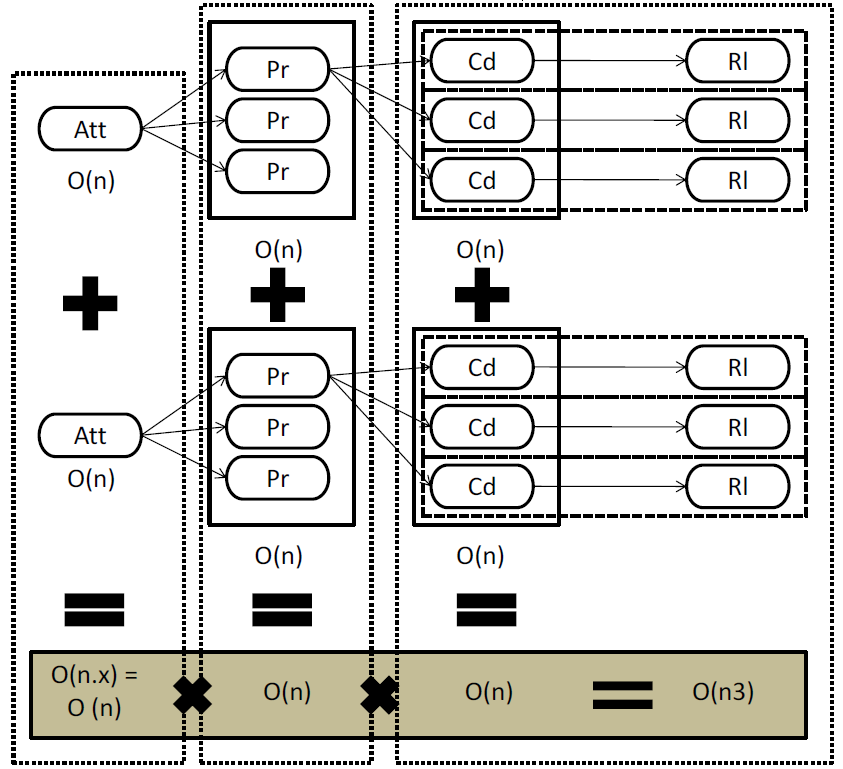
\includegraphics[width=0.8\textwidth]{../figures/calculo_pon.png}
  \smallskip
  \caption*{Fonte: \citeonline{msc_Banaszewski_2009}}
  \label{fig:calculo_pon}
\end{figure}

\section{Conceitos de programação ou desenvolvimento em
  PON}\label{sec:conceitos_pon}

Desde as subseções \ref{sec:reatividade} até \ref{sec:agregacao} se apresentam
os diversos conceitos de programação ou desenvolvimento em PON, introduzidos com
o objetivo de facilitar o desenvolvimento de aplicações em PON, sendo que não
necessariamente cada materialização (\textit{i.e.}, implementação) do PON as
contemplam na sua totalidade.

\subsection{Reatividade das entidades}\label{sec:reatividade}

No PON, a reatividade das suas entidades é um conceito central. Neste âmbito, as
entidades reativas do PON conseguem gerar as notificações pontuais entre si, de
acordo com a alteração dos seus estados, que ditam o fluxo de execução do
programa em PON. De maneira geral, a reatividade presente nas entidades
definidas no metamodelo do PON proporciona uma execução livre de avaliações
lógico-causais redundantes e desnecessárias. 

A reatividade das entidades na cadeia de notificações do PON permite evitar a
redundância temporal ao avaliar as expressões lógico-causais somente após a
mudança de estado dos \textit{Attributes} e suas respectivas \textit{Premises}.
Ainda, esta reatividade encontra respaldo no fato de \textit{Conditions} poderem
compartilhar a colaboração de \textit{Premises}, o que evita a redundância
estrutural nas avaliações lógico-causais. Por fim, a reatividade em PON pode ser
melhorada de algumas formas, como por meio de tabelas \textit{hash} nos
Attributes, permitindo que \textit{Premises} recebam notificações de apenas
certos estados de interesse, mas não dos estados que não são de seus interesses
\cite{msc_Banaszewski_2009}. Estes cenários de notificação de \textit{Premises}
tanto com uma lista encadeada simples como com uma tabela \textit{hash} são
ilustrados na Figura \ref{fig:hash_not}, onde um \textit{Attribute}
\textit{atSignal} tem seu estado alterado de vermelho (\textit{RED}) para verde
(\textit{GREEN}), sendo que as setas partindo do \textit{Attribute} representam
as notificações realizadas \cite{msc_Banaszewski_2009}.

\begin{figure}[!htb]
  \centering
  \caption{Notificações baseadas em lista encadeada e tabela \textit{hash}}
  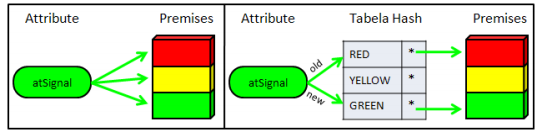
\includegraphics[width=\textwidth]{../figures/hash_not.png}
  \smallskip
  \caption*{Fonte: \citeonline{msc_Banaszewski_2009}}
  \label{fig:hash_not}
\end{figure}

\subsection{Renotificações}

Os \textit{Attributes}, pela sua definição, notificam as \textit{Premises}
apenas quando seu estado é alterado. Porém, em determinados cenários, pode haver
a necessidade de execução de uma \textit{Rule} mesmo quando não há a alteração
no estado dos \textit{Attributes}. Tome-se como exemplo uma \textit{Rule}
responsável (via sua \textit{Action} e dada \textit{Instigation}) pela
instigação da execução de determinado \textit{Method} que precise ser
constantemente reinstigado enquanto a \textit{Condition} daquela \textit{Rule}
estiver verdadeira \cite{msc_Banaszewski_2009}.

Neste tipo de contexto que se faz necessário implementar alguma solução, como o
chamado mecanismo de renotificações. No diagrama de atividades da Figura
\ref{fig:renotif_activity}, é ilustrado o processo de decisão para a geração de
notificação em entidades que suportam o mecanismo de renotificação. Com a
utilização do mecanismo de renotificações, a notificação é gerada mesmo quando
não ocorre uma mudança de estado. À luz da Figura \ref{fig:renotif_activity},
pode-se definir uma frequência para definir (\textit{setar}) estado, permitindo
que a cadeia de notificações seja animada com uma dada cadência
\cite{msc_Banaszewski_2009}.

\begin{figure}[!htb]
  \centering
  \caption{Diagrama de atividades do processo de renotificação}
  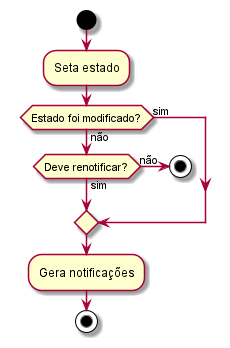
\includegraphics[width=0.4\textwidth]{../out/diagrams/renotification/renotif.png}
  \smallskip
  \caption*{Fonte: Autoria própria}
  \label{fig:renotif_activity}
\end{figure}

\FloatBarrier

Para exemplificar mais precisamente esse cenário de renotificações, tome-se o
exemplo de \textit{Rule} para um alarme apresentado na Figura
\ref{fig:ex_rule_renotif}. Neste caso é considerado que o mecanismo de ativação
da sirene, implementado por meio de \textit{mtRingSirenMilliseconds}, permanece
ativado por um tempo limitado após ser instigado (100 ms neste exemplo). Deste
modo se torna necessário que a cada nova atribuição de valor para
\textit{atStatus} do \textit{FBE} Sensor, seja executada novamente a
\textit{Rule}, o que é feito com a utilização do mecanismo de renotificação.

\begin{figure}[!htb]
  \centering
  \caption{\textit{Rule} que depende do mecanismo de renotificações}
  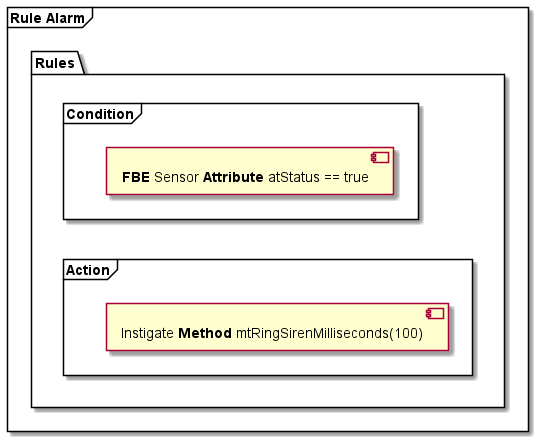
\includegraphics[width=0.6\textwidth]{../out/diagrams/rule_renotif/rules_renotif.png}
  \smallskip
  \caption*{Fonte: Autoria própria}
  \label{fig:ex_rule_renotif}
\end{figure}

\subsection{\textit{Keeper}}

O mecanismo de renotificações, apesar de útil, pode ser bastante
computacionalmente custoso, porque ele causa um aumento no número de
notificações geradas pelo sistema, aumentando o tempo de execução das
aplicações. Desta forma, outra estratégia alternativa desenvolvida de moto a
atender a necessidade de execução de uma \textit{Rule} mesmo quando não há a
alteração no estado dos \textit{Attributes} foi o padrão \textit{Keeper}.
Diferente das renotificações, com o \textit{Keeper} não é necessária uma nova
notificação para executar a \textit{Rule}, mas sim a execução da \textit{Rule}
pode ser explicitamente requisitada a ser executada quantas vezes for
necessário, enquanto a mesma se mantenha aprovada \cite{muchalski_2012}.

Entretanto, o principal problema da adoção dessa estratégia é que a
responsabilidade da execução das \textit{Rules} é passada inteiramente ao
desenvolvedor, visto que as \textit{Rules} não mais são executadas no momento em
que são aprovadas, mas sim apenas quando requisitada explicitamente no código.
Isso é necessário de forma a evitar a execução duplicada das \textit{Rules}. O
uso do \textit{Keeper} é exemplificado no Código \ref{cod:keeper}, onde é
possível observar na linha 3 onde a execução da \textit{Rule} \textit{rlProduct}
é explicitamente requisitada.

\begin{lstlisting}[numbers=left,
  stepnumber=1, caption = {Exemplo de
  uso do padrão \textit{Keeper}}, float=htb, source = {Adaptado de \citeonline{muchalski_2012}}, label =
  {cod:keeper}]
void Result::UpdateProduct() {
  prProduct->setCalue(production->getProductId());
  rlProcudt->execute();
}
\end{lstlisting}


\subsection{Entidades impertinentes}

Ainda no contexto da reatividade das entidades, podem existir cenários nos quais
as notificações de certas entidades podem ser consideradas desnecessárias. Isso
pode ocorrer em situações nas quais um \textit{Attribute}, que apesar de não ser
determinante sozinho para a aprovação de uma \textit{Rule} em um dado contexto,
apresenta constantes mudanças de estado, disparando o fluxo de notificações
novamente a cada variação em seu estado. Nesse caso as notificações
desnecessárias impactam negativamente no desempenho da aplicação PON
\cite{msc_Ronszcka_2012}.

A Figura \ref{fig:pr_imp_1} ilustra um cenário de entidades impertinentes, com
um exemplo hipotético de controle de temperatura, com dois \textit{Attributes},
nomeadamente \textit{atStatus} e \textit{atTemperature}. Nesse caso,
\textit{atTemperature} vai variar constantemente, enquanto \textit{atStatus} vai
variar muito ocasionalmente. Porém, a \textit{Condition} da \textit{Rule} somente
será aprovada quando \textit{atStatus} possuir o valor \textit{true} e
\textit{atTemperature} possuir um dado valor. Nesse cenário dado, as
notificações geradas por \textit{atTemperature} seriam impertinentes em sua
maioria.

\begin{figure}[!htb]
  \centering
  \caption{Alterações de estado com \textit{Attribute} impertinente ativo}
  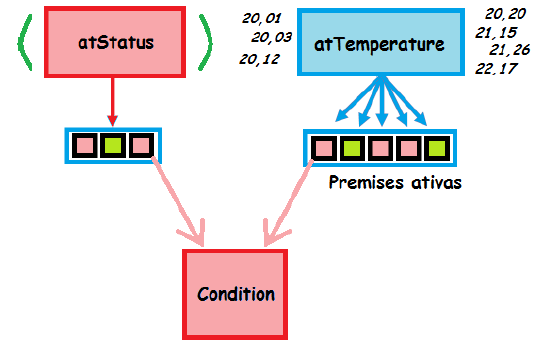
\includegraphics[width=0.55\textwidth]{../figures/pr_imp_1.png}
  \smallskip
  \caption*{Fonte: \citeonline{msc_Ronszcka_2012}}
  \label{fig:pr_imp_1}
\end{figure}

Neste cenário em pauta, o \textit{Attribute} \textit{atTemperature} é
categorizado como impertinente por sua mudança estaticamente não aprovar a
\textit{Condition} da \textit{Rule}, logicamente em função da mudança largamente
mais discreta de seu parceiro de conjunção, o pertinente \textit{atStatus}.
Deste modo, para evitar notificações desnecessárias, suas \textit{Premises} não
deveriam receber notificações temporariamente, sendo que as notificações do
\textit{atTemperature} para tais \textit{Premises} seriam desabilitadas até
segunda ordem. A Figura \ref{fig:pr_imp_2} ilustra o mesmo cenário acima, porém
com \textit{atTemperature} sendo tido como um \textit{Attribute} impertinente
para com \textit{Premises}, tendo suas notificações temporariamente
desabilitadas.

\begin{figure}[!htb]
  \centering
  \caption{Alterações de estado com \textit{Attribute} impertinente desativado}
  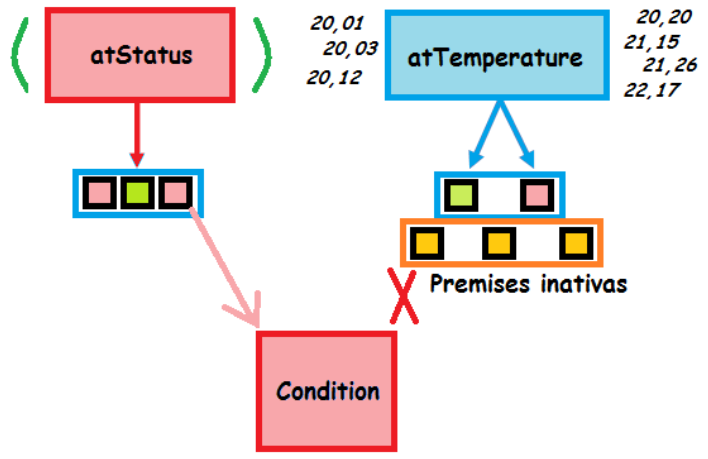
\includegraphics[width=0.55\textwidth]{../figures/pr_imp_2.png}
  \smallskip
  \caption*{Fonte: \citeonline{msc_Ronszcka_2012}}
  \label{fig:pr_imp_2}
\end{figure}


Nesse âmbito a \textit{Condition} fica responsável por reativar temporariamente
as \textit{Premises} relativas a \textit{Attributes} impertinentes, de modo a
voltar receber notificações destas, quando o conjunto de \textit{Premises}
pertinentes para sua aprovação forem satisfeitas. Essa reativação temporária,
ilustrada na Figura \ref{fig:pr_imp_3}, torna capaz a aprovação da
\textit{Condition}. Por fim, após a aprovação e execução da \textit{Rule},
volta-se a desativar o \textit{Attribute} impertinente no contexto da
\textit{Rule} em questão. Desta forma, o \textit{Attribute} impertinente
voltaria a ignorar \textit{Premises} da \textit{Condition} daquela \textit{Rule}
até que fosse requisitado novamente pela \textit{Condition}
\cite{msc_Ronszcka_2012}.

\begin{figure}[!htb]
  \centering
  \caption{Alterações de estado com \textit{Attribute} impertinente reativado}
    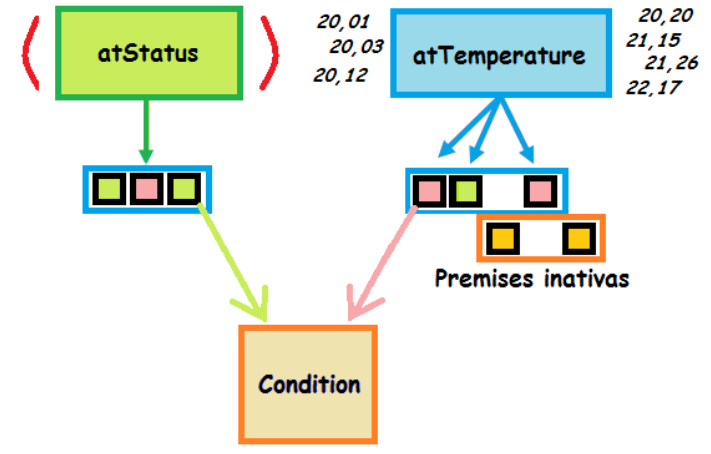
\includegraphics[width=0.55\textwidth]{../figures/pr_imp_3.png}
  \smallskip
  \caption*{Fonte: \citeonline{msc_Ronszcka_2012}}
  \label{fig:pr_imp_3}
\end{figure}

\FloatBarrier

A definição de impertinência das entidades pode acontecer em dois momentos,
feita a priori ou em tempo de execução. Esses dois modos de impertinência são
chamados de impertinência estática e impertinência dinâmica. A impertinência
estática é de responsabilidade do desenvolvedor, de modo que a entidade já é
definida como impertinente no momento da compilação, enquanto a impertinência
dinâmica não é definida pelo desenvolvedor e sim por um mecanismo em tempo de
execução que seja capaz de detectar a impertinência das entidades a luz de dados
estatísticos.

\subsection{Compartilhamento de entidades}\label{sec:compartilhamento}

O uso do compartilhamento (de colaboração) de entidades pode ser considerado uma
boa prática do PON tanto da perspectiva da facilidade de desenvolvimento como
para o ganho de desempenho. O compartilhamento de entidades como
\textit{Conditions} e \textit{Premises} oferece ganhos de desempenho ao eliminar
a criação de estruturas redundantes e, com isso, também reduz o número de
notificações desnecessárias \cite{msc_Ronszcka_2012}. O ganho em facilidade de
desenvolvimento, por sua vez, é dado pelo fato do compartilhamento de entidades
acontecer de forma natural ao desenvolvedor durante o desenvolvimento das
\textit{Rules} do programa em PON. Quando o desenvolvedor escreve o código em
PON, seria um cenário comum diferentes \textit{Rules} estarem relacionadas às
mesmas \textit{Premises}, \textit{Conditions} ou \textit{Instigations}, as quais
seriam compartilhadas já em tempo de construção do programa.

O compartilhamento de entidades é um meio útil para a resolução do
problema de redundância estrutural, conceito introduzido na reflexão sobre
paradigmas da Seção \ref{sec:paradigmas}. Em suma, a redundância estrutural
ocorre, por exemplo, quando o conhecimento sobre um estado resultante da
avaliação de dada expressão lógica (\textit{e.g.}, comparação de uma variável com uma
constante) não é compartilhado entre outras expressões causais pertinentes,
causando reavaliações desnecessárias \cite{msc_Banaszewski_2009}. O
compartilhamento de colaboração de entidades evita avaliações redundantes, ao fornecer um meio
para se compartilhar os resultados das avaliações lógicas comuns a várias
expressões causais \cite{msc_Banaszewski_2009}.

\begin{figure}[!htb]
  \centering
  \caption{Declaração de \textit{Premises} do exemplo do alarme}
  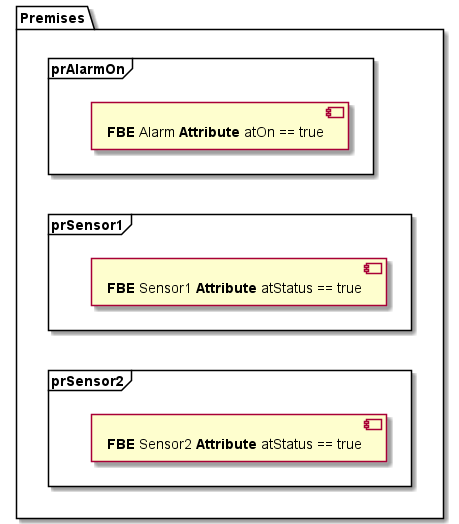
\includegraphics[width=0.45\textwidth]{../out/diagrams/shared_premises/premises.png}
  \smallskip
  \caption*{Fonte: Autoria própria}
  \label{fig:premises_shared_ex}
\end{figure}

Para exemplificar o compartilhamento de entidades, é expandido o exemplo do
alarme, introduzido na Seção \ref{sec:estado_arte_pon}, para ter duas
\textit{Rules} e com dois \textit{FBEs} relativos aos sensores, porém apenas um
\textit{FBE} para o alarme. Neste caso, existem três \textit{Premises},
mostradas na Figura \ref{fig:premises_shared_ex}, e duas \textit{Rules},
mostradas na Figura \ref{fig:rules_shared_ex}. Nesse cenário observa-se que
ambas as \textit{Rules}, dependem da mesma \textit{Premise} \textit{prAlarmOn},
que neste caso é uma entidade cuja colaboração é compartilhada para com as
\textit{Rules}, sendo que ambas são notificadas pelas \textit{Premise} em
questão quando pertinente.

\begin{figure}[!htb]
  \centering
  \caption{Declaração de \textit{Rules} utilizando \textit{Premises}
    compartilhadas}
  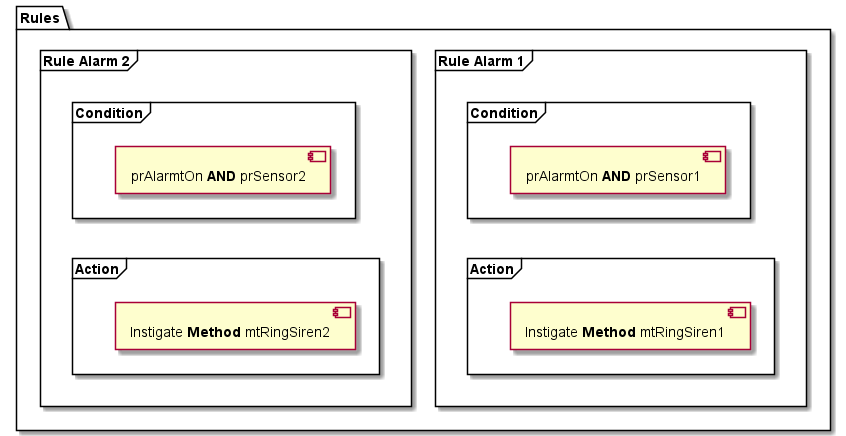
\includegraphics[width=0.8\textwidth]{../out/diagrams/rules_example/rules.png}
  \smallskip
  \caption*{Fonte: Autoria própria}
  \label{fig:rules_shared_ex}
\end{figure}

\subsection{Resolução de conflitos}\label{sec:conflitos}

Um conflito acontece quando duas atividades diferentes dependem de um mesmo
recurso compartilhado, o qual deve ser usado exclusivamente
\cite{doc_simao_2005}. Uma das características do PON é ser também orientado a
regras, sendo que conflitos entre regras podem surgir quando duas ou mais
\textit{Rules} são aprovadas com base em estado de recurso exclusivo. Outra
característica do PON é justamente permitir a execução de forma desacoplada e
concorrente dos elementos do seu modelo, permitindo paralelismos e distribuições
conforme o ambiente em que a aplicação PON seja executada. Nesse âmbito, é
importante a identificação e resolução de conflitos originados dessa execução
desacoplada de aprovação e execução de \textit{Rules} \cite{msc_pordeus_2017}.

No PON, mais precisamente, o conflito ocorre quando duas ou mais \textit{Rules}
referenciam um mesmo \textit{FBE} e demandam exclusividade de acesso a este
\textit{FBE} (como para o caso de modificar \textit{Attributes} deste
\textit{FBE}). Neste caso, apenas uma das \textit{Rules} poderia ser executada
por vez, fazendo o acesso exclusivo a este \textit{FBE}, o que leva ele a ser um
FBE exclusive neste contexto dado. Ainda, neste âmbito de conflitos, a resolução
de conflitos em ambientes monoprocessados ocorre de modo a estabelecer a ordem
de execução das \textit{Rules}. Já em ambientes multiprocessados, a resolução de
conflitos é necessária para evitar o acesso concorrente ao mesmo recurso
\cite{msc_valenca_2012,msc_Banaszewski_2009}.

Nos ambientes monoprocessados pode ser aplicado um escalonador de \textit{Rules}
que utiliza estruturas de dados lineares (\textit{e.g.}, pilha, filha ou lista)
\cite{msc_Banaszewski_2009}. Esse modelo, exemplificado na Figura
\ref{fig:conflitos}, recebe as \textit{Rules} na ordem em que são aprovadas e as
executa de acordo com a estratégia de resolução de conflito escolhida, o que
seria assaz similar a resolução conflitos em geral de sistemas baseados em
regras \cite{msc_Banaszewski_2009}. Isto dito, as diferentes estratégias de
resolução de conflitos para ambientes monoprocessados são listadas abaixo:

\begin{itemize}
  \item \textit{Breadth} ou largura: escalonamento \textit{First In First Out}
        (FIFO), primeiro a entrar é o primeiro a sair, no qual as \textit{Rules}
        são executadas na mesma ordem que são aprovadas. Pode ser usada uma
        estrutura de dados do tipo fila para este propósito.
  \item \textit{Depth} ou profundidade: escalonamento \textit{Last In First Out}
        (LIFO), último a entrar é o último a sair, no qual as \textit{Rules}
        são executadas começando sempre pela última \textit{Rule} aprovada. Pode
        ser usada uma estrutura de dados do tipo pilha para este propósito.
  \item \textit{Priority} ou prioridade: escalonamento baseado na prioridade definida para
        cada \textit{Rule}.
  \item \textit{No one} ou nenhum: a \textit{Rule} é executada imediatamente ao ser
        aprovada.
\end{itemize}

\begin{figure}[!htb]
  \centering
  \caption{Modelo centralizado de resolução de conflitos na estratégia
    \textit{Breadth}} 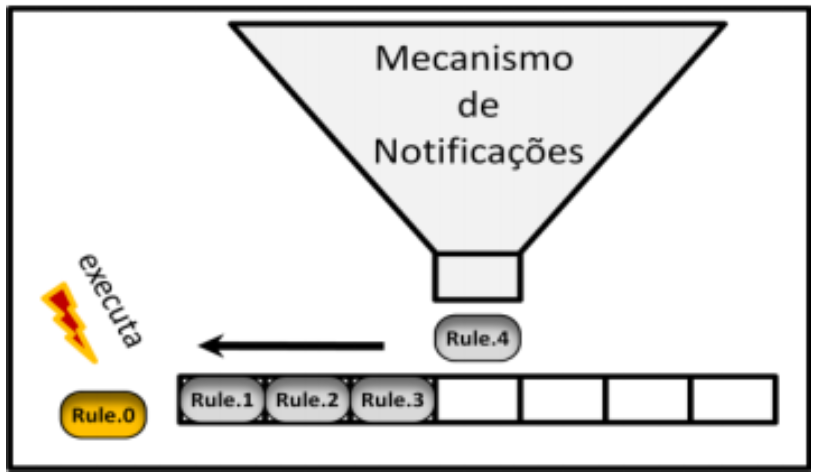
\includegraphics[width=0.7\textwidth]{../figures/conflitos.png}
  \smallskip
  \caption*{Fonte: \citeonline{msc_Banaszewski_2009}}
  \label{fig:conflitos}
\end{figure}

\FloatBarrier

Apesar deste modelo ser uma solução eficiente para ambientes monoprocessados,
ele não se mostra adequado para ambientes \textit{multicore} por não apresentar
um mecanismo que permita o escalonamento apropriado da execução das
\textit{Rules}. \citeonline{msc_Banaszewski_2009} então propõe tal mecanismo que
execute o escalonamento de forma eficiente. Para que este mecanismo de
escalonamento seja integrado ao modelo de resolução de conflitos, é necessário
alterar a forma pela qual as \textit{Rules} são executadas neste modelo. Assim, ao invés
de uma \textit{Rule} aprovada instigar a execução imediata da mesma, essa deve
repassar o controle da execução da respectiva \textit{Rule} para o componente
escalonador de \textit{Rules}. Quando a \textit{Rule} é aprovada, ao invés de ser
executada imediatamente, ela é adicionada a uma fila de execução, considerando a
prioridade de execução das respectivas \textit{Rules}. Por sua vez, essas
\textit{Rules} são executadas de forma escalonada por uma \textit{pool} de
executores, com um número de executores pré-definidos, que permite a execução
simultânea de múltiplas \textit{Rules}.

\subsection{\textit{Master Rule}}

Este conceito estabelece um mecanismo de dependência entre \textit{Rules}. Podem
existir cenários nos quais diferentes \textit{Rules} dependem do mesmo conjunto
de \textit{Premises} compartilhadas para sua aprovação, as quais notificariam
todas as entidades interessadas em suas mudanças de estado. Nesse caso as
notificações desnecessárias podem ser evitadas caso essas \textit{Premisses}
notifiquem uma única \textit{Rule}, ao invés de todas as interessadas. Essa
\textit{Rule}, quando aprovada, fica responsável por notificas as demais
\textit{Rules} interessadas e, portanto, dependentes daquela. Nesse cenário é
criada uma dependência entre as \textit{Rules}, na qual a \textit{Master Rule} é
capaz de notificar outras \textit{Rules} \cite{msc_Ronszcka_2012}. Esse
mecanismo traz benefícios em questões de desempenho e facilidade na composição
de aplicações, porque a dependência entre as \textit{Rules}, por meio do
conceito de \textit{Master Rule}, reduz as notificações geradas pelas
\textit{Premises} ao direcionar as notificações apenas para a \textit{Master
Rule} \cite{msc_Ronszcka_2012}.

Para exemplificar o conceito de \textit{Master Rule} é expandido o exemplo do
alarme explorado na Seção \ref{sec:compartilhamento}, com duas \textit{Rules} e
com dois \textit{FBEs} para os sensores, porém agora considerando que uma das
\textit{Rules}, chamada \textit{rlAlarm2}, depende de três \textit{Premises}
(\textit{prAlarmOn}, \textit{prSensor1} e \textit{prSensor2}), sendo que duas
destas \textit{Premises} fazem parte da composição de outra \textit{Rule},
chamada \textit{rlSensor1}, de modo que este cenário pode ser construído por
meio do uso de uma \textit{Master Rule}. Considere-se as mesmas três
\textit{Premises} da Figura \ref{fig:premises_shared_ex}, aplicadas nas
\textit{Rules} da Figura \ref{fig:master_rule}. Pela aplicação da \textit{Master
Rule}, a aprovação da \textit{rlAlarm2} só acontece após a \textit{rlAlarm1}
também ser aprovada.

\begin{figure}[!htb]
  \centering
  \caption{Exemplo de aplicação de \textit{Master Rule}}
  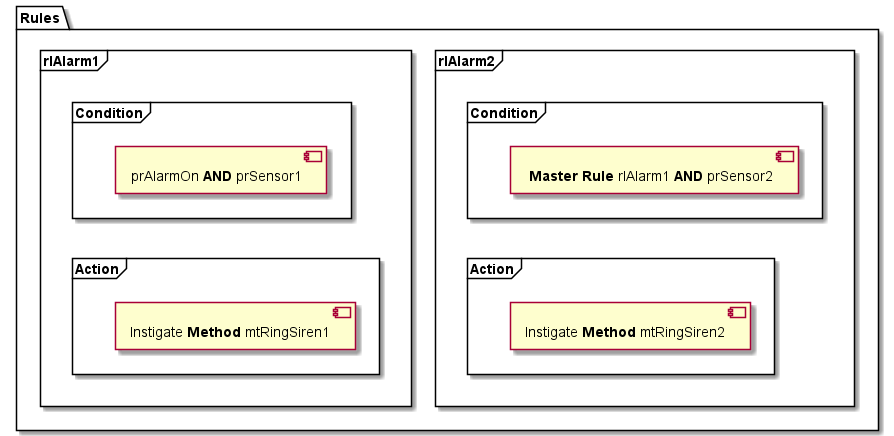
\includegraphics[width=0.8\textwidth]{../out/diagrams/master_rule/rules.png}
  \smallskip
  \caption*{Fonte: Autoria própria}
  \label{fig:master_rule}
\end{figure}

\subsection{\textit{Formation Rules} - Regras de Formação}

O conceito de \textit{Formation Rules} (ou Regra de Formação) do PON é um
reaproveitamento das \textit{Formation Rules} do Controle Orientado a
Notificações (CON), o predecessor do PON \cite{msc_simao_2001}. Cada
\textit{Formation Rule} permite a criação de \textit{Rules} específicas com base
na representação genérica de uma \textit{Rule}. Esse conceito é útil quando o
conhecimento causal de uma Rule é comum para diferentes conjuntos de instâncias
de \textit{FBEs}, ou seja, um conjunto de \textit{Rules} específicas se
diferencia apenas nas instâncias referenciadas \cite{doc_ronszcka_2019}.

A título de exemplo tome-se um cenário hipotético de um sistema de alarmes, no
qual existem as entidades usuários e alarmes (\textit{FBE User} e \textit{FBE
Alarm}). A responsabilidade do sistema seria de avisar cada usuário sobre a
ativação de cada alarme conectado. Para isso seria necessário replicar essa
condição para cada combinação de usuário e alarme (\textit{e.g.}, \textit{user1
x alarm1, user1 x alarm2, user2 x alarm1, user2 x alarm2 etc.}), o que torna o
processo custoso e propenso a erros \cite{doc_ronszcka_2019}.

Com a aplicação do conceito de \textit{Formation Rules} se torna possível a
declaração do conhecimento lógico-causal da \textit{Rule} de forma genérica, com
base nos tipos dos \textit{FBEs}, ao invés das instâncias pontuais de cada um.
Assim, em tempo de compilação, seria feita a composição das \textit{Rules} para
cada combinação de instâncias \cite{doc_ronszcka_2019}. Isso permite tornar a
replicação de \textit{Rules} uma tarefa automática, minimizando a possibilidade
de erros e facilitando o trabalho do desenvolvedor, além de promover maior
legibilidade do código em geral, ao remover a duplicação de código similar
repetido \cite{doc_ronszcka_2019}.

A Figura \ref{fig:formation_rule} ilustra uma representação de uma
\textit{Formation Rule} que pode ser adotada para gerar as instâncias das
\textit{Rules} referentes a um cenário de automatização do controle de veículos.
Neste caso a \textit{Formation Rule} define a \textit{Rule} que deve ser
aplicada a todos os carros e cruzamentos, onde o veículo só pode acelerar caso o
sinal esteja no estado verde e não hajam pessoas andando no cruzamento.

\begin{figure}[!htb]
  \centering
  \caption{Representação de uma \textit{Formation Rule}}
  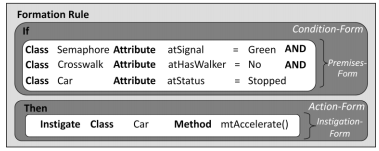
\includegraphics[width=0.7\textwidth]{../figures/formation_rule.png}
  \smallskip
  \caption*{Fonte: \citeonline{msc_Banaszewski_2009}}
  \label{fig:formation_rule}
\end{figure}

Uma \textit{Formation Rule} é mais genérica do que uma \textit{Rule}
tradicional. Para sua descição é utilizado o sufixo \textit{Form}, que define as
lógicas que é utilizada como base para instanciar de forma efetiva cada uma das
entidades do PON. As suas entidades \textit{Form} somente analisam se o
\textit{FBE} é de uma determinada classe. Uma \textit{Formation Rule} filtra e
cria combinações de \textit{FBEs}, onde cada combinação resulta na criação de
uma \textit{Rule} independente. Em suma, uma \textit{Formation Rule} aplica
conceitos genéricos a fim de criar \textit{Rules} específicas, mantendo a
capacidade de notificação entre os objetos colaboradores. A função principal da
\textit{Formation Rule} é gerar automaticamente a partir de um modelo várias
instâncias de Rules que compartilham a semântica deste modelo. 


\subsection{\textit{FBE Rules}}\label{sec:fbe_rule}

De maneira geral, o conceito de agregações de \textit{Rules} em \textit{FBEs} é
um conceito próximo ao das \textit{Formation Rules}, sendo um caso particular
das \textit{Formation Rules} no qual a \textit{Rule} está relacionada a apenas
um tipo de \textit{FBE}, enquanto nas \textit{Formation Rules} a \textit{Rule}
pode estar relacionada a vários \textit{FBE} \cite{msc_santos_2017}. Uma
\textit{FBE Rule} é uma \textit{Rule} que possui escopo local em seu
\textit{FBE}, e todas as instâncias deste \textit{FBE} possuem,
obrigatoriamente, uma instância da \textit{Rule} em questão
\cite{doc_ronszcka_2019}.

A título de exemplo considera-se a aplicação do alarme com seu respectivo
sensor. Para a execução de vários alarmes seria necessário replicar as
\textit{Rules} para cada instância. Porém, com a utilização do conceito de
\textit{FBE Rules}, essa replicação pode ser feita de modo automático com a
declaração da \textit{Rule} como uma \textit{FBE Rule} do \textit{FBE} do
alarme. A Figura \ref{fig:fbe_rule} ilustra este cenário.

\begin{figure}[!htb]
  \centering
  \caption{Exemplo de aplicação de \textit{FBE Rules}}
  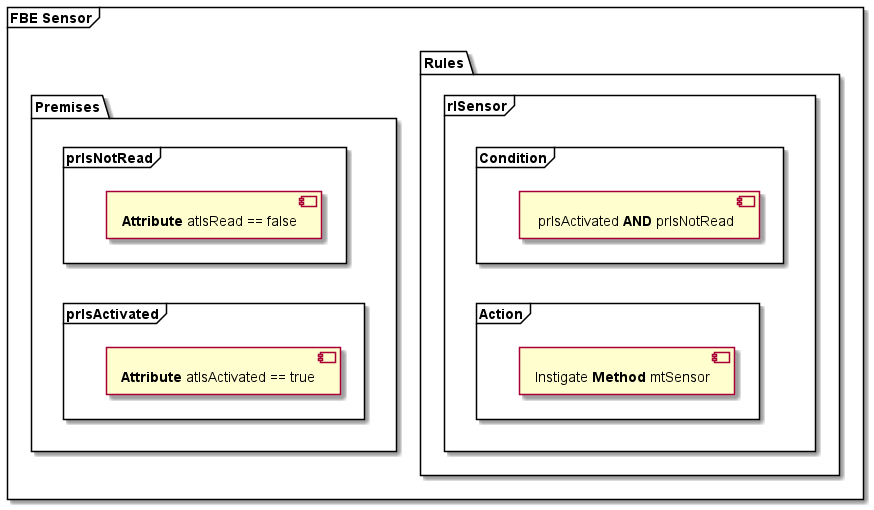
\includegraphics[width=0.8\textwidth]{../out/diagrams/fbe_rule/rules.png}
  \smallskip
  \caption*{Fonte: Autoria própria}
  \label{fig:fbe_rule}
\end{figure}

\subsection{Agregação entre \textit{FBEs}}\label{sec:agregacao}

Outro conceito pertinente ao PON é possibilidade de criar agregações entre
\textit{FBEs}, permitindo a criação de \textit{FBEs} compostos sem a necessidade
de duplicação de estruturas. Esse conceito permite otimizações na redução de
código, assim como também facilita a descrição de programas em PON, tanto de
forma textual como gráfica \cite{doc_ronszcka_2019}. Com isso, espera-se atingir
níveis de organização mais efetivos, melhorando particularmente a escrita e a
legibilidade de programas baseados no PON.

Esta forma de estruturação facilita a construção de \textit{Rules} que podem ser
compostas internamente aos \textit{FBEs}, sendo o caso das \textit{FBE Rules}.
Neste caso a agregação de \textit{FBEs} permite a criação de \textit{Rules}
utilizando todos os \textit{FBEs} agregados. 

%Como no caso do exemplo da Seção \ref{sec:fbe_rule}, no qual o \textit{FBE}
%\textit{Alarm} agrega o \textit{FBE} Sensor, de forma que cada instância do
%\textit{FBE Alarm} cria uma instância do seu \textit{FBE Sensor} agregado.

\subsection{Resumo dos Conceitos de Programação do PON}

Nas seções anteriores foram apresentados diversos conceitos de programação do
PON. De forma a facilitar o entendimento sobre tais conceitos, o Quadro
\ref{tab:resumo_conceitos} apresenta um resumo de cada um desses conceitos.
Isto é feito de forma a apresentar de forma simplificada e centralizada o
conhecimento sobre os conceitos de programação do PON.

É importante ressaltar que apesar de todas as materializações do PON buscarem
aplicar todos esses conceitos, raramente isso acontece. Alguns conceitos de
programação foram introduzidos por materializações mais recentes do PON, de modo
que, naturalmente, as implementações que precedem a introdução de determinado
conceito não o materializam. Ainda assim, mesmo em materializações mais recentes,
limitações de ordem técnica ou conceitual podem impedir a implementação de todos
esses conceitos.

\begin{tabframed}[!htb]
\centering
\caption{Resumo de conceitos de programação do PON}
\begin{tabularx}{\textwidth}{l|X}
Conceito                              & Definição                                                                                                                                  \\ \hline\hline
Reatividade das entidades             & Entidades são capazes de gerar notificações pontuais de forma espontânea na alteração de estado                                            \\ \hline
Renotificações                        & Entidades podem gerar notificações de forma forçada, mesmo sem alteração nos seus estados                                                  \\ \hline
\textit{Keeper}                       & Controle manual de execução das \textit{Rules}, permitindo execução de uma \textit{Rule} múltiplas vezes enquanto aprovada                 \\ \hline
Impertinência                         & Supressão seletiva de notificações de determinadas entidades, podendo ocorrer de forma estática ou dinãmica                                \\ \hline
Compartilhamento de entidades         & Utillização compartilhada de entidades com conhecimento em comum com outras entidades, reduzindo o número de entidades únicas no sistema   \\ \hline
\textit{Master Rule}                  & Relação de depedência entre \textit{Rules} com conhecimento lógico-causal em comum                                                         \\ \hline
\textit{Formation Rules}              & Criação de \textit{Rules} baseadas na representação genérica de uma \textit{Rule} relativa ao tipo dos \textit{FBEs}                       \\ \hline
\textit{FBE Rules}                    & Definição de \textit{Rules} no corpo do \textit{FBE}, instanciando uma \textit{Rule} independente para cada instância de dado \textit{FBE} \\ \hline
Agregação entre \textit{FBEs}         & Criação de \textit{FBEs} compostos de outros \textit{FBEs}                                                                                 \\ \hline
\end{tabularx}
\caption*{Fonte: Autoria própria}
\label{tab:resumo_conceitos}
\end{tabframed}

\clearpage
\section{Materializações do PON em software}\label{sec:frameworks}

O PON apresenta materializações tanto em software quanto em hardware
\cite{doc_linhares_2015,doc_Kerschbaumer_2018,doc_ronszcka_2019,doc_Schutz_2019}.
Entretanto, este trabalho foca nas implementações em software e não hardware.
Nas implementações em software, há tanto implementações em \textit{frameworks}
como também por meio de linguagem de programação própria, por meio da chamada
Tecnologia LingPON. Enquanto a linguagem de programação via Tecnologia LingPON
se constitui em estado da arte por ainda ser consideravelmente prototipal, o
conjunto de \textit{frameworks} se constituem no estado da técnica por parte
deles se encontrar em estado estável de desenvolvimento.

As implementações por meio de \textit{frameworks} existem de forma a oferecer
uma interface de programação de aplicativos (API - \textit{Application
Programming Interface}) que possibilite o desenvolvimento de aplicações seguindo
o modelo do PON, modificando, portanto, a maneira como estas linguagens operam,
justamente permitindo e conduzindo-lhes a operarem de forma orientada a
notificações. As seções seguintes apresentam cada uma destas materializações em
software em maiores detalhes, sendo que a primeira subseção desta presente seção
se dedica aos \textit{frameworks} para o PON desenvolvidos em linguagem de
programação C++.

\subsection{\textit{Frameworks} PON C++}

A materialização do PON em C++ conta com mais de uma única implementação, sendo
que cada uma destas materializações foi construída com base nas materializações
anteriores, cada uma com sua proposta de melhoria específica. Estas diferentes
materializações são o \textit{Framework} PON C++ Prototipal, \textit{Framework}
PON C++ 1.0, \textit{Framework} PON C++ 2.0 e \textit{Framework} PON C++ 3.0.
Além dessas materializações, também há o prototipal JuNOC++, desenvolvido por
\citeonline{chierichi_2020} com base no trabalho da dissertação de
\citeonline{msc_Ronszcka_2012}. Estas materializações são exploradas
individualmente em maior detalhe nas seções seguintes.

%\footnote{Também há a implementação
%do \textit{Framework} JuNOCpp, desenvolvido por Gustavo Chierici, como uma
%reimplementação do \textit{Framework} PON C++ 2.0, com base no trabalho da
%dissertação de mestrado do Ronszcka em 2012, disponível em
%\url{https://github.com/GustavoChierici/JuNOCpp}}

\subsubsection{\textit{Framework} PON C++ Prototipal}\label{sec:fw_prot}

A primeira implementação do PON sobre o formato de \textit{framework}, o chamado
\textit{Framework} PON C++ Prototipal, foi proposta por Simão em 2007
\cite{pat_simao_2008,simao_2012a}. Esta versão prototipal do \textit{framework}
deriva dos esforços de sua dissertação de mestrado e tese de doutorado no âmbito
do metamodelo do Controle Orientado a Notificações (CON), o qual foi aplicado
sobre a ferramenta de simulação de sistema de manufatura ANALYTICE II
\cite{doc_simao_2005,simao_2009}.

A Figura \ref{fig:mira_alvo} é apresentada com o objetivo de ilustrar uma
aplicação desenvolvida com a aplicação do \textit{Framework} PON C++ Prototipal.
Neste exemplo de implementação, toma-se uma aplicação intitulada Mira ao Alvo,
na qual as entidades miras e as entidades alvos são representadas
respectivamente por arqueiros e maçãs, sendo que há uma maçã para cada arqueiro.
Isto dito, este cenário é descrito sob a forma de \textit{FBEs} e \textit{Rule}
no Código \ref{cod:mira_alvo_fbe}.

\noindent
\begin{minipage}{.45\textwidth}
  \centering
  \captionof{figure}{Cenário do Mira ao Alvo}
  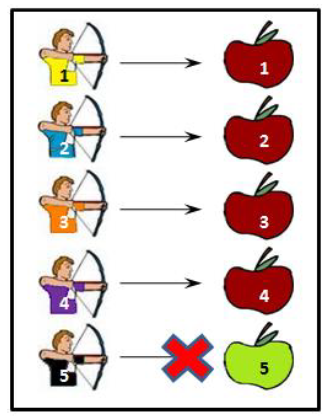
\includegraphics[width=0.95\textwidth]{../figures/mira_alvo.png}
  \captionof{figure}*{Fonte: \citeonline{msc_Banaszewski_2009}}
  \label{fig:mira_alvo}
\end{minipage}\hfill
\begin{minipage}{.45\textwidth}
  \begin{lstlisting}[caption = {\textit{FBEs} e \textit{Rule} para cenário do Mira ao Alvo},
    source = {\citeonline{chierichi_2020}}, language=nopl,
    label = {cod:mira_alvo_fbe}]
fbe Archer
  public boolean atStatus = false
  public integer atIdentity = 0
end_fbe
fbe Apple
  public boolean atAppleColor = false
  public integer atIdentity = 0
  public boolean atIsCrossed = false
  private method mtStatusOff
    attribution
      this.atIsCrossed = true
    end_attribution
  end_method
end fbe
inst
 Archer archer
 Apple apple
end_inst
rule rlShootApple
  condition
      premise prIdentity
        apple.atIdentity == archer.atIdentity
      end_premise
      and
      premise prColor
        apple.atColor == true
      end_premise
      and
      premise prAppleStatus
        apple.atStatus == true
      end_premise
      and
      premise prArcherStatus
        archer.atStatus == true
      end_premise
      and
      premise prAppleIsNotCrossed
        apple.atIsCrossed == false
      end_premise
  end_condition
  action sequential
      instigation sequential
        call apple.mtStatusOff()
      end_instigation
  end_action
end_rule
  \end{lstlisting}
\end{minipage}

Em termos de implementação, no \textit{Framework} PON C++ Prototipal, cada
arqueiro e maçã é representado por um objeto notificante na forma de FBE
(\textit{i.e.}, um Elemento da Base de Fatos), os quais interagem de acordo com
a avaliação de expressões causais pertinentes na forma de objetos \textit{Rules}
(\textit{i.e.}, uma \textit{Rule}) \cite{msc_Banaszewski_2009}. Essa
implementação em foco é mostrada no Código \ref{cod:fwprot_ex}.

\begin{lstlisting}[caption = {Exemplo de programa com o \textit{framework} C++ prototipal},
  source = {Adaptado de \citeonline{msc_Banaszewski_2009}},
  label = {cod:fwprot_ex}, float=htb]
//Premises
prAppleColorRead = new AgentePremissa(appleList->at(i)->atAppleColor, True);
prAppleColorRead->conectaPredBooleano(&comparaBooleanos);
prAppleStatusTrue = new AgentePremissa(appleList->at(i)->atAppleStatus, True);
prAppleStatusTrue->conectaPredBooleano(&comparaBooleanos);
prArcherStatusTrue = new AgentePremissa(archerList->at(i)->atArcherStatus, True);
prArcherStatusTrue->conectaPredBooleano(&comparaBooleanos);
//Conditions
AgenteCondicao* cdFireApple;
acFireApple = new AgenteAcao();
acFireApple->conectaAgenteOrdem(appleList->at(i)->mtChangeToGreen);
//Method
mtChangeToGreen = new AgenteMetodoGen<Apple>(&Apple::ChangeToGreen);
//Instigation
aitChangeToGreen = new AgenteOrdem(mtChangeToGreen);
//Rule
AgenteRegra* rlFireApple;
rlFireApple = new AgenteRegra(cdFireApple, acFireApple);
\end{lstlisting}

\vspace{-1cm}
\subsubsection{\textit{Framework} PON C++ 1.0}

O \textit{Framework} PON C++ 1.0 foi implementado por Banaszewski em 2009, com a
proposta de facilitar e melhorar a composição de programas em PON. A estrutura
de implementação desta versão do \textit{framework} é constituída por dois
principais pacotes de classes, o pacote \textit{Core} e o pacote
\textit{Application}, conforme ilustrado na Figura \ref{fig:fw_pkg}. O pacote
\textit{Core} contém as classes que modelam as entidades do metamodelo do PON,
enquanto o pacote \textit{Application} contém as classes utilizadas para a
instanciação de uma aplicação em PON, usando as entidades do pacote
\textit{Core} \cite{msc_Banaszewski_2009}.

\begin{figure}[!htb]
  \centering
  \caption{Estrutura do \textit{framework} C++ 1.0}
  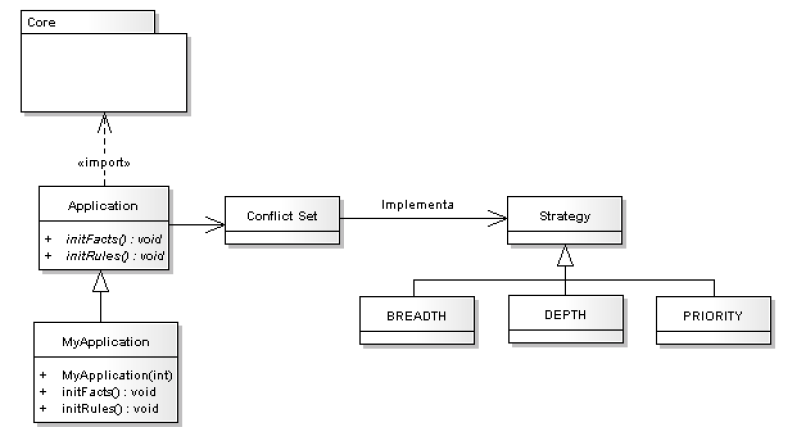
\includegraphics[width=0.85\textwidth]{../figures/fw1_structure.png}
  \caption*{Fonte:
    \citeonline{msc_Banaszewski_2009}}
  \label{fig:fw_pkg}
\end{figure}

Nesta estrutura, a classe \textit{MyApplication} é um exemplo de implementação
que seria definida pelo programador com base na classe abstrata
\textit{Application} do \textit{framework}. A classe \textit{Application}
representa um modelo de inicialização padrão para aplicações em PON, por meio da
construtora da classe, na qual é definida a estratégia de resolução de
conflitos, bem como dos métodos \textit{initFacts} e \textit{initRules}, os
quais são respectivamente usados para concentrar a instanciação dos
\textit{FBEs} e \textit{Rules} \cite{msc_Banaszewski_2009}.

Em resumo, a construção de aplicações utilizando o \textit{Framework} PON C++
1.0 se baseia em torno da especialização da classe \textit{Application}, que
contém os métodos necessários para a inicialização das estruturas do PON. Um
exemplo de aplicação para o mesmo cenário Mira ao Alvo, já descrito
anteriormente na Seção \ref{sec:fw_prot}, agora com o \textit{framework} C++
1.0, é mostrado no Código \ref{cod:fw1_ex}.

\begin{lstlisting}[caption = {Exemplo de programa com o \textit{framework} C++ 1.0},
source = {Adaptado de \citeonline{msc_Banaszewski_2009}},
   label = {cod:fw1_ex}, float=htb]
for ( iteratorArcher = archerList->begin(), iteratorApple = appleList->begin(); 
      iteratorArcher != archerList->end();
      ++iteratorArcher, ++iteratorApple)
{	
  Instigation* it = new Instigation((*iteratorApple)->mtStatusOff);
  RuleObject* rlFireApple = new RuleObject("",scheduler, Condition::CONJUNCTION);

  rlFireApple->addPremise((*iteratorApple)->atIdentity,
                          (*iteratorArcher)->atIdentity, Premise::EQUAL, false);
  rlFireApple->addPremise((*iteratorApple)->atAppleColor,
                          Boolean::TRUE_NOP, Premise::EQUAL, false);
  rlFireApple->addPremise((*iteratorApple)->atAppleStatus,
                          Boolean::TRUE_NOP, Premise::EQUAL, false);
  rlFireApple->addPremise((*iteratorApple)->atAppleIsCrossed,
                          Boolean::FALSE_NOP, Premise::EQUAL, false);
  rlFireApple->addPremise((*iteratorArcher)->atArcherStatus,
                          Boolean::TRUE_NOP, Premise::EQUAL, false);
  rlFireApple->addPremise(gun->atIsFired,
                          Boolean::TRUE_NOP, Premise::EQUAL, false);
  rlFireApple->addPremise(gun->atIdentityOfBullet,
                          cont, Premise::EQUAL, false);

  rlFireApple->addInstigation(it);
  rlFireApple->end();
  cont++;
}
\end{lstlisting}

Isto dito, com as melhorias propostas, foi possível obter ganhos de desempenho
quando comparado o \textit{Framework} PON C++ 1.0  para com o \textit{Framework}
PON C++ prototipal. Para avaliar o desempenho destas duas versões foi executada
a aplicação do cenário Mira ao Alvo, variando a porcentagem de \textit{Rules}
aprovadas em cada iteração, no qual a aplicação com o \textit{Framework} PON C++
1.0 chega a atingir tempos de execução 60\% menores que os da aplicação com o
\textit{Framework} PON C++ prototipal. Na Figura \ref{fig:fw1_vs_prot} é
mostrado o resultado para a execução de 10.000 iterações, nela \enquote{Versão Antiga}
se refere ao \textit{framework} C++ Prototipal e \enquote{Versão Nova} se refere ao
\textit{framework} C++ 1.0 \cite{msc_Banaszewski_2009}.

\begin{figure}[!htb]
  \centering
  \caption{Comparação do desempenho do \textit{framework} C++ 1.0 com o
  \textit{framework} C++ Prototipal}
  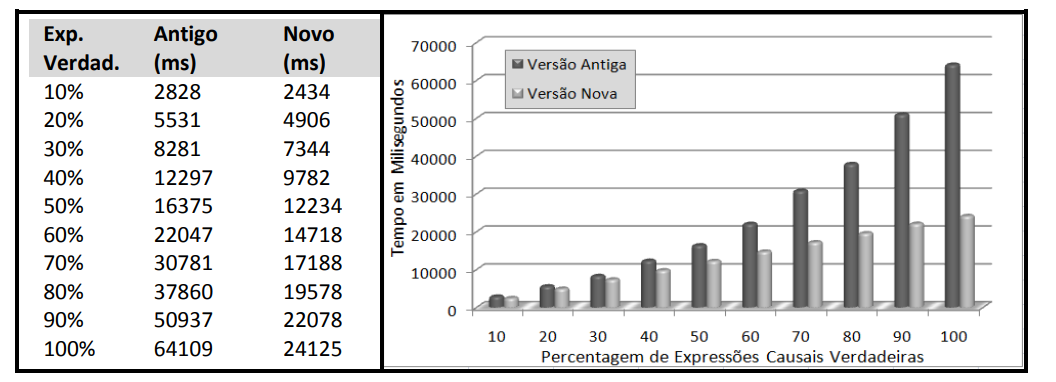
\includegraphics[width=0.9\textwidth]{../figures/fw1_vs_prot.png}
  \caption*{Fonte:
  \citeonline{msc_Banaszewski_2009}}
  \label{fig:fw1_vs_prot}
\end{figure}

\FloatBarrier

\subsubsection{\textit{Framework} PON C++ 2.0}\label{sec:fw2_revisao}

Subsequentemente, uma nova versão do \textit{framework} foi introduzida a partir
dos esforços de trabalhos de mestrado de Valença e Ronszcka em 2012
\cite{msc_valenca_2012,msc_Ronszcka_2012}. A estrutura da versão 2.0, ilustrada
na Figura \ref{fig:fw2_struct}, ainda mantém uma estrutura muito similar àquela
introduzida na versão 1.0, adotando a mesma estrutura de pacotes
\cite{msc_Ronszcka_2012}. Essa versão é considerada a principal materialização
estável para o desenvolvimento de aplicações no PON, por possuir o maior grau de
maturidade e estabilidade entre as materializações existentes para implementação
do PON em \textit{software} \cite{doc_ronszcka_2019}.

\begin{figure}[!htb]
  \centering
  \caption{Estrutura do \textit{framework} C++ 2.0}
  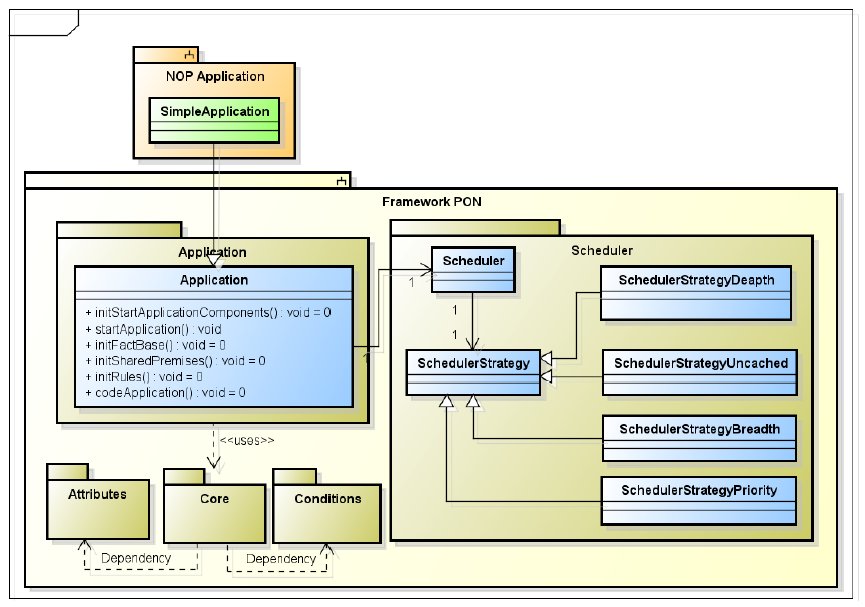
\includegraphics[width=0.8\textwidth]{../figures/fw2_structure.png}
  \caption*{Fonte:
    \citeonline{msc_valenca_2012}}
  \label{fig:fw2_struct}
\end{figure}

Nesta implementação, Ronszcka propôs a utilização de padrões de projeto para o
desenvolvimento do \textit{framework} \cite{msc_Ronszcka_2012}, enquanto Valença
efetuou 'otimizações' (\textit{i.e.}, aprimoramentos) por meio do uso de
estruturas de dados com implementação própria (nomeadamente \textit{NOPVECTOR},
\textit{NOPHASH} e \textit{NOPLIST}), com melhor desempenho computacional que as
estruturas da STL. Com as melhorias propostas, foi possível obter ganhos de
desempenho quando comparado o Framework PON C++ 2.0 com o \textit{Framework} PON
C++ 1.0 \cite{msc_valenca_2012}. 

Ainda, com base nesta versão de \textit{framework}, foi desenvolvida uma aplicação
gráfica que possibilita a criação de \textit{FBEs} e \textit{Rules}, chamada
\textit{Wizard} PON, a qual é mostrada na Figura \ref{fig:wizard}. Com o auxílio
dessa aplicação é possível fazer a construção de um programa em PON em alto
nível, de maneira visual. Com essa ferramenta é possível escrever a estrutura do
programa em PON que passa então por um processo de geração de código para o
\textit{Framework} PON C++ 2.0 \cite{msc_valenca_2012}.

\begin{figure}[!htb]
  \centering
  \caption{\textit{Wizard} PON} 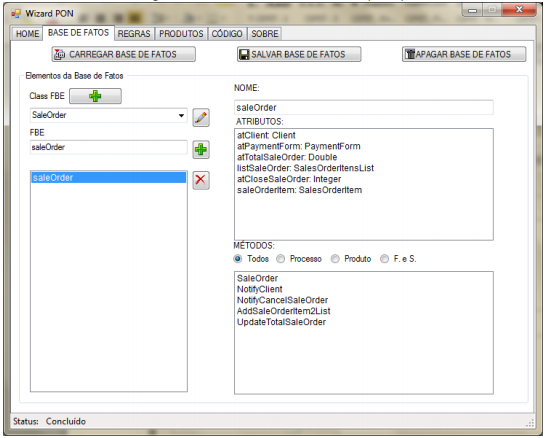
\includegraphics[width=0.8\textwidth]{../figures/wizard.png}
  \caption*{Fonte: \citeonline{msc_valenca_2012}}
  \label{fig:wizard}
\end{figure}

Um exemplo de aplicação para o mesmo cenário Mira ao Alvo, já descrito
anteriormente na Seção \ref{sec:fw_prot}, mas agora com o \textit{Framework} PON
C++ 2.0 é mostrado no Código \ref{cod:fw2_ex}. Nota-se a sintaxe bastante
similar à do \textit{Framework} PON C++ 1.0, porém com a adição do uso do padrão
de projeto \textit{factory}. 

\begin{lstlisting}[caption = {Exemplo de programa com o \textit{framework} C++ 2.0},
source = {Adaptado de \citeonline{msc_valenca_2012}},
  label = {cod:fw2_ex}, float=htb]
Premise* p = elementsFactory->createPremise(gun->atIsFired, true, Premise::EQUAL, false);
for ( int i = 0; i < appleList->size(); i++ ){
  Apple* appleTmp = appleList->at(i);
  Archer* archerTmp = archerList->at(i)

  RuleObject* rlFireApple = elementsFactory->createRuleObject(
                              "rule", scheduler, Condition::CONJUNCTION);
  rlFireApple->addPremise(
    elementsFactory->createPremise(
      appleTmp->atIdentity,archerTmp->atIdentity, Premise::EQUAL, false));
  rlFireApple->addPremise(
    elementsFactory->createPremise(
      appleTmp->atAppleColor, true, Premise::EQUAL, false));
  rlFireApple->addPremise(
    elementsFactory->createPremise(
      appleTmp->atAppleStatus, true, Premise::EQUAL, false));
  rlFireApple->addPremise(
    elementsFactory->createPremise(
      appleTmp->atAppleIsCrossed, false, Premise::EQUAL, false));
  rlFireApple->addPremise(
    elementsFactory->createPremise(
      archerTmp->atArcherStatus, true, Premise::EQUAL, false));
  rlFireApple->addPremise(p);
  rlFireApple->addInstigation(
    elementsFactory->createInstigation(appleTmp->mtStatusOff));
}
\end{lstlisting}

A mesma aplicação Mira ao Alvo é utilizada para comparar o desempenho do
\textit{Framework} PON C++ 2.0 com o \textit{framework} C++ 1.0. Nestes testes, a
utilização do \textit{Framework} PON C++ 2.0 foi com a estrutura de dados
\textit{PONVECTOR} apresentou em média 30\% do tempo de processamento utilizado
em relação ao \textit{Framework} PON C++ 1.0, o que corresponderia a um ganho de
desempenho de cerca três vezes, conforme observado na Figura
\ref{fig:fw2_vs_fw1}. Nessa figura \enquote{\textit{Framework} Original} se refere  ao
\textit{Framework} PON C++ 1.0.

\begin{figure}[!htb]
  \centering
  \caption{Comparação do desempenho do \textit{Framework} PON C++ 2.0 com o
  \textit{Framework} PON C++ 1.0}
  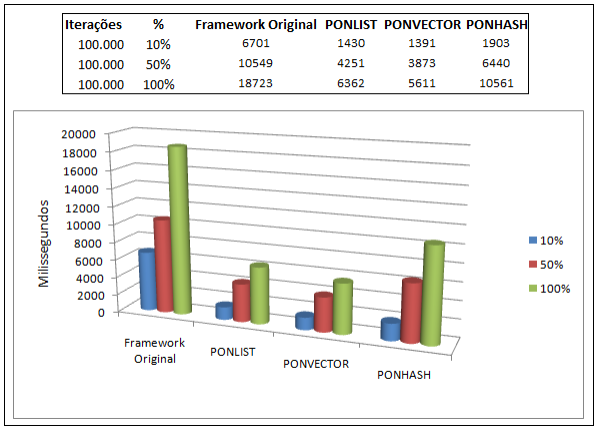
\includegraphics[width=0.7\textwidth]{../figures/fw2_vs_fw1.png}
  \caption*{Fonte: \citeonline{msc_valenca_2012}}
  \label{fig:fw2_vs_fw1}
\end{figure}

\FloatBarrier

\subsubsection{\textit{Framework} PON C++ 3.0}\label{sec:fw3}

Tanto a versão do \textit{Framework} PON C++ 1.0 como o \textit{Framework} PON
C++ 2.0 consideram apenas a execução em ambientes monoprocessados e
monoprocesso/\textit{single thread} em sua concepção. Ou seja, \textit{Frameworks}
PON C++ 1.0 e 2.0 não consideram execução em ambiente \textit{multithread},
multiprocesso e, menos ainda, \textit{multicore}. Nesse sentido, foi proposto o
\textit{Framework} PON C++ 3.0. Esta versão é uma extensão da implementação do
\textit{Framework} PON C++ 2.0 incluindo a execução de conjuntos de
\textit{Rules} por meio de \textit{threads} independentes. Ademais, ele fornece
uma maneira de se paralelizar elementos do PON de forma transparente, em nível
de \textit{thread} para ambientes \textit{multicore} \cite{belmonte_2012}.

A estrutura do \textit{Framework} PON C++ 3.0 é apresentada na Figura
\ref{fig:fw3_struct}. Nela, os pacotes \textit{Application} e \textit{Core} são
os mesmos do \textit{Framework} PON C++ 2.0. Ainda com base nessa figura e na
Figura \ref{fig:fw2_struct}, podem ser destacadas algumas diferenças. Dentre
elas, há a criação do \textit{NOPVectorMulticore}, uma especialização do
\textit{NOPVECTOR} desenvolvido especialmente para trabalhar com aplicações
\textit{multicore}, agindo como um iterador das entidades do PON de forma
otimizada, reduzindo o uso do \textit{cache} da aplicação
\cite{belmonte_2012,schutz_2018}. Também há a adição do pacote
\textit{Multicore}, cujas entidades são detalhadas abaixo:

\begin{itemize}
  \item \textit{SynchronizedQueue}: Fila que armazena as entidades do PON a
        serem executadas, de forma sincronizada, em cada \textit{core} do
        processador \cite{belmonte_2012,schutz_2018}.
  \item \textit{CoreController}: Classe responsável por enfileirar as entidades
        do PON quando o \textit{CoreControllersManager} registra uma
        notificação. Também é responsável pela execução paralelizada das
        \textit{Premises}, \textit{Conditions} e \textit{Methods} em cada
        \textit{core} \cite{belmonte_2012,schutz_2018}.
  \item \textit{CoreControllersManager}: Classe responsável por criar a
        instância do \textit{CoreController} para cada \textit{core} do
        processador. Durante a execução responsável por registrar as
        notificações recebidas pelas entidades do PON \cite{belmonte_2012,schutz_2018}.
  \item \textit{Thread}: Classe de execução que controla o uso das
        \textit{threads}, por meio do uso de mecanismos de exclusão mútua. Para
        sua implementação é utilizada a biblioteca \textit{pthreads}
        \cite{belmonte_2012,schutz_2018}.
  \item \textit{SleepCondition}: Classe que possui métodos para auxiliar o
        controle da execução da fila de entidades do PON. Para sua implementação
        é utilizada a biblioteca \textit{pthreads} \cite{belmonte_2012,schutz_2018}.
\end{itemize}

Conforme descrito acima à luz da Figura \ref{fig:fw3_struct}, novas classes
foram criadas para suportar o mecanismo \textit{multithread} e usar paralelismo
em nível de \textit{thread} quando em um contexto de dois ou mais núcleos ou
\textit{cores} (\textit{multicores}), utilizando inclusive a API \textit{pthreads}. Esta
API fornece um conjunto de bibliotecas com recursos de controle e sincronização
de \textit{threads}, por meio dos conceitos de exclusão mútua (\textit{mutex})
para controlar o acesso e a execução de entidades compartilhadas entre as
\textit{threads}.

\begin{figure}[!htb]
  \centering
  \caption{Estrutura do \textit{framework} C++ 3.0} 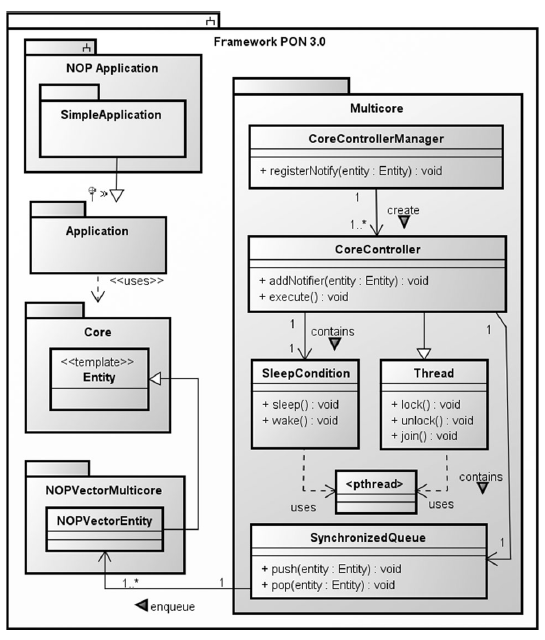
\includegraphics[width=.65\textwidth]{../figures/fw_30.png}
  \caption*{Fonte:
    \citeonline{schutz_2018}}
  \label{fig:fw3_struct}
\end{figure}

A classe \textit{CoreControllermanager} é responsável por instanciar cada
\textit{FBE} da aplicação em um núcleo específico, de forma que as entidades da
cadeia de notificações sejam distribuídas entre os núcleos disponíveis de forma
controlada \cite{doc_Schutz_2019}. A fim de respeitar a execução correta das
entidades PON em cada núcleo, a classe \textit{CoreController} gerencia uma fila
de entidades a serem executadas, a \textit{SynchronizedQueue}. Assim, uma
entidade notificada vai para esta fila de execução e, assim que um núcleo do
processador esteja disponível, uma entidade é removida da fila e executada,
segundo o processo ilustrado na Figura \ref{fig:fw3_flow}

Além disso, durante o desenvolvimento do \textit{Framework} PON C++ 3.0
persebeu-se a existência de um problema de \textit{stack overflow} (estouro de
pilha), possívelmente presente em todos os \textit{frameworks} em C++
anteriores. O \textit{stack overflow} acontece quando ocorre a chamada de muitas
funções em sequência, sem nunca retornar, o que pode ser causado, por exemplo,
por uma sequência muito grande de notificações que realimenta o ciclo de
notificações indefinidamente. Subsequentemente no \textit{Framework} PON C++ 3.0
foi criado um desacoplamento do mecanismo de notificações, onde o
\textit{Method} não é instigado diretamente pela entidade notificante, mas sim
colocada dentro de uma fila de notificações dentro de uma entidade controladora,
o \textit{CoreController}, quebrando assim esse ciclo de execução indefinido.

\begin{figure}[!htb]
  \centering
  \caption{Diagrama de atividades do controle de entidades do \textit{framework}
    C++ 3.0}
  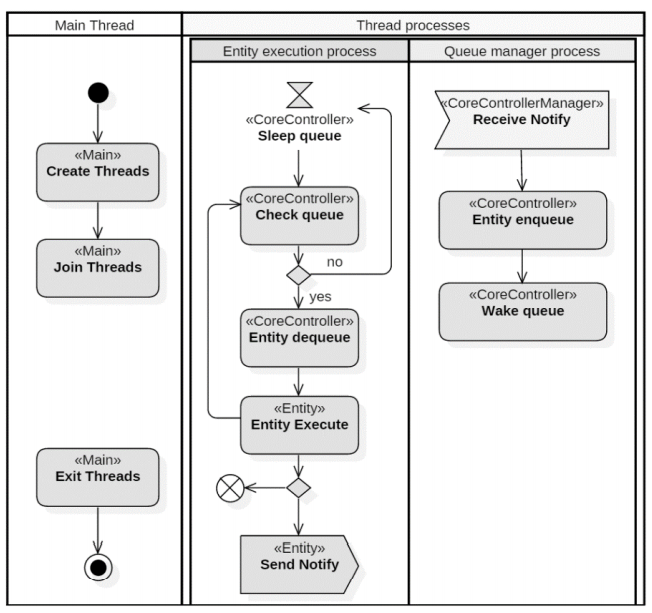
\includegraphics[width=.55\textwidth]{../figures/fw30_flow.png}
  \caption*{Fonte: \citeonline{schutz_2018}}
  \label{fig:fw3_flow}
\end{figure}

O processo de balanceamento da carga de trabalho do \textit{software} executado
pelo \textit{CoreControllerManager} é realizado de acordo com o método chamado
Motor de Balanceamento para Inferência Orientada a Notificações (\textit{Load
balancing engine for Notification-Oriented Inference - LobeNOI}), apresentado na
Figura \ref{fig:lobenoi}. Neste método primeiramente uma etapa de análise e
alocação dinâmica verifica o número de núcleos disponíveis do processador e
realiza a alocação inicial da aplicação, subsequentemente a etapa de análise e
alocação dinâmica monitora a utilização dos núcleos e realiza o balanceamento da
carga de trabalho em si por meio da realocação das entidades da aplicação
\cite{belmonte_2016}.

\begin{figure}[!htb]
  \centering
  \caption{Visão geral do método \textit{LobeNOI}} 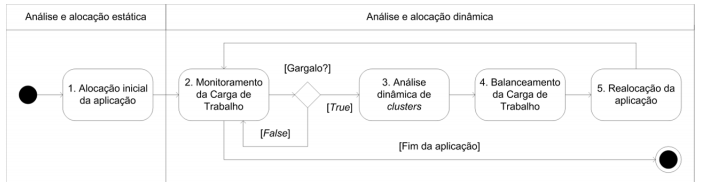
\includegraphics[width=\textwidth]{../figures/lobenoi.png}
  \caption*{Fonte:
  \citeonline{belmonte_2016}}
  \label{fig:lobenoi}
\end{figure}

Ainda com base na implementação original do \textit{Framework} PON C++ 3.0 foi
implementado o NeuroPON em software paralelo \cite{schutz_2018}, o qual consiste
em uma nova arquitetura de treinamento e execução de Redes Neurais Artificias
(RNA) baseados em PON. O NeuroPON acrescenta algumas estruturas novas sobre o
\textit{Framework} PON C++ 3.0, de modo a permitir a sua construção sobre este
\textit{framework}.

A estrutura das entidades adicionadas pela NeuroPON é mostrada no diagrama da
Figura \ref{fig:neuro_struct}. Essas estruturas modelam os neurônios como
\textit{FBEs}, com \textit{Rules} e afins agregadas tratando de sua lógica dita
neural, bem como a classe de controle da rede neural em si como uma
\textit{NOPApplication} naturalmente com outras \textit{Rules} pertinentes.

\begin{figure}[!htb]
  \centering
  \caption{Estrutura do NeuroPON}
  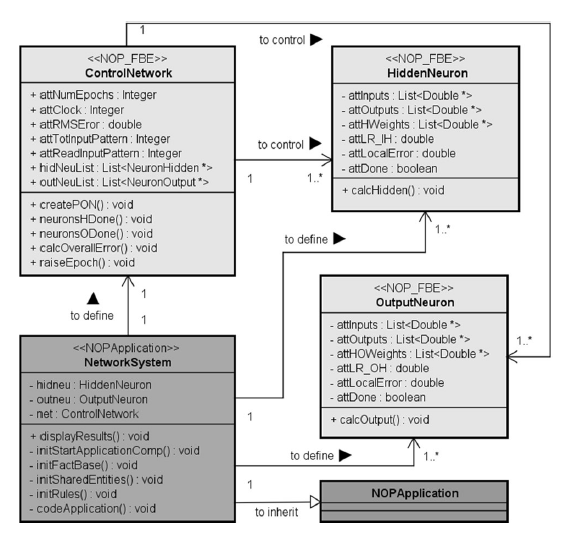
\includegraphics[width=.6\textwidth]{../figures/neuropon_struct.png}
  \caption*{Fonte: \citeonline{schutz_2018}}
  \label{fig:neuro_struct}
\end{figure}

Conforme descrito acima, o \textit{Framework} PON C++ 3.0 possui mecanismos que
visam a organização e balanceamento da execução do programa de forma automática,
ou seja, sem a intervenção explícita do desenvolvedor, o qual alcançou bons.
Entretanto, o \textit{Framework} PON C++ 3.0 não alcançou os benefícios de
desempenho esperados pelo uso de paralelização em NeuroPON, tendo o tempo de
execução consideravelmente superior ao do \textit{Framework} PON C++ 3.0.

Tais problemas de desempenho se deram mais precisamente em uma aplicação
desenvolvida com a NeuroPON para o treinamento de uma RNA com
\textit{Multiplayer Perception} (MLP) utilizando o método de \textit{Back
Propagation} (BP) \cite{schutz_2018}. Os experimentos realizados com o
\textit{Framework} PON C++ 3.0 permitem observar a taxa de ocupação dos núcleos,
sendo mantido acima de 60\% em cada núcleo durante a execução da aplicação,
conforme mostrado na Figura \ref{fig:core_usage_cpp3}\footnote{Experimentos
realizados com um processador Core i7-3770 3.5 Ghz, 32 GB de memória RAM DDR3
1357MHz, com o sistema operacional Linux Ubuntu 16.04 LTS 64 bits.}. Entretanto,
isto não aportou um bom desempenho global em função das idiossincrasias da
arquitetura do NeuroPON, como a alta conectividade entre os seus constituintes,
não ser bem suportada pela abordagem do \textit{Framework} PON C++ 3.0 conforme
detalhado na tese de \citeonline{schutz_2018}.

No final das contas, no contexto dado, a execução de forma paralelizada trouxe
um aumento do tempo de execução do programa em PON. De forma geral, mecanismos
de controle de execução paralela (\textit{i.e.}, \textit{mutex},
\textit{threads}) causam um aumento do tempo de processamento. A utilização de
um número pequeno de neurônios nos experimentos faz com que as operações
paralelizadas sejam realizadas de forma muito rápida, fazendo com que a
aplicação gaste a maior parte do tempo nos mecanismos de controle, de modo que a
paralelização não traz melhoria nos tempos de execução \cite{schutz_2018}. Os
resultados, apresentados na Figura \ref{fig:pon_multi}, mostram que conforme
aumenta o número de núcleos utilizados, maior o tempo de execução
\cite{schutz_2018}.

\begin{figure}[!htb]
  \centering
  \caption{Taxa de utilização dos núcleos da CPU no treinamento de RNA MLP com método BP}
  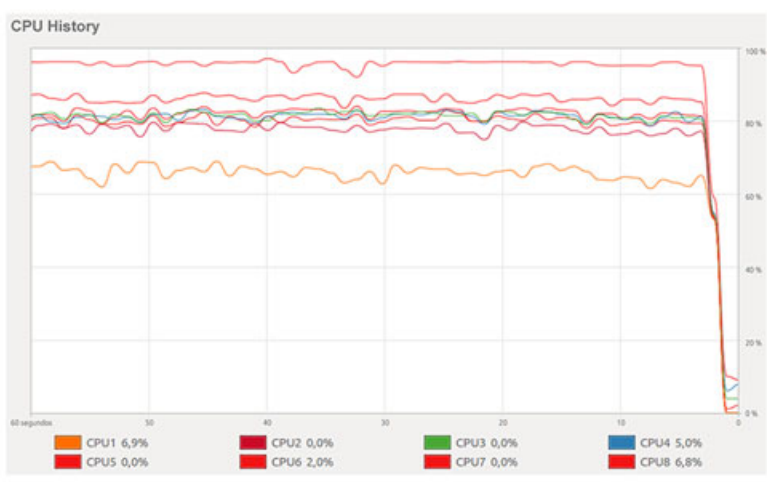
\includegraphics[width=.65\textwidth]{../figures/core_usage_cpp3.png}
  \caption*{Fonte: \citeonline{schutz_2018}}
  \label{fig:core_usage_cpp3}
\end{figure}

Os resultados da NeuroPON paralela em \textit{Framework} PON C++ 3.0 poderiam
não depor contra o \textit{Framework} PON C++ 3.0 em si, mas contra a NeuroPON
finalmente. Entretanto, experimentos com a NeuroPON em outro \textit{framework}
demonstrariam que o problema enfim não seria nela, mas sim no Framework PON C++
3.0. Os resultados a NeuroPON neste outro \textit{framework} serão considerados
subsequentemente neste trabalho e se encontram na dissertação de mestrado de
\citeonline{negrini_2019}.

\begin{figure}[!htb]
  \centering
  \caption{Tempos de execução (em milissegundos) do treinamento de ANN MLP com método BP}
  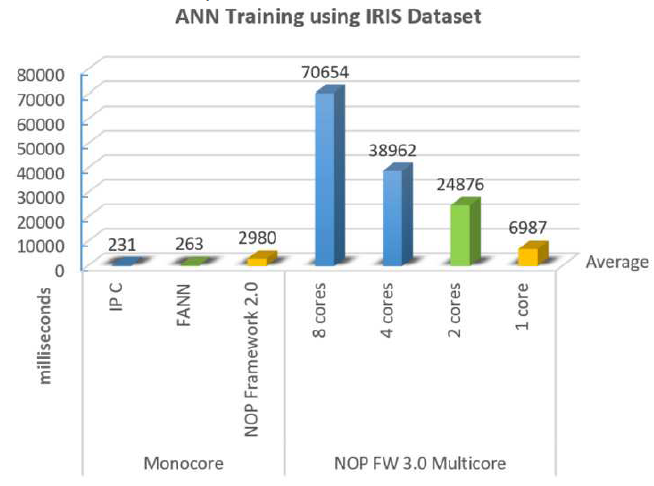
\includegraphics[width=.55\textwidth]{../figures/pon_multi_fix.png}
  \caption*{Fonte: \citeonline{schutz_2018}}
  \label{fig:pon_multi}
\end{figure}

\subsubsection{JuNOC++}

Todos os \textit{frameworks} em C++ apresentados até agora foram construídos
como evoluções com base nas versões anteriores. Além destes \textit{frameworks}
em C++, também há o JuNOC++ (\textit{Just a Notification Oriented} C++). Este
\textit{framework} se destaca por surgir não como uma evolução dos
\textit{frameworks} anteriores, mas sim como uma tentativa de
\citeonline{chierichi_2020} de criar um \textit{framework} do PON com base na
fundamentação apresentada na dissertação de \citeonline{msc_Banaszewski_2009}.
Desta forma, \citeonline{chierichi_2020} propõe uma estrutura que deixa de ser
mera reprodução dos \textit{frameworks} existentes, mas sim um novo
\textit{framework} independente com foco em programação em alto nível,
expressividade e desempenho.
%\footnote{A implementação do \textit{Framework}
%JuNOC++ está disponível em \url{https://github.com/GustavoChierici/JuNOCpp}}.

Do ponto de vista da estrutura do \textit{framework}, o JuNOC++ utiliza uma
estrutura baseada no pacote \textit{Core} do \textit{Framework} PON C++ 1.0,
incluindo melhorias principalmente observadas pela utilização de
\textit{templates} para a implementação de \textit{Attributes} e
\textit{Premises}. Esta estrutura de classes é ilustrada na Figura
\ref{fig:class_junoc}.

\begin{figure}[!htb]
  \centering
  \caption{Diagrama de classes do JuNOC++}
  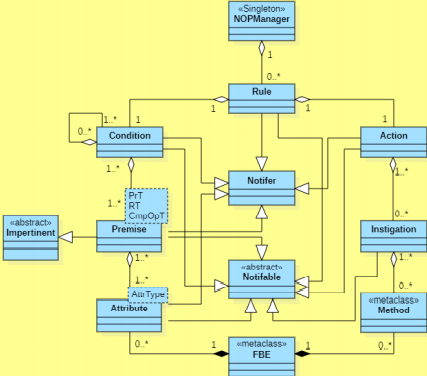
\includegraphics[width=.7\textwidth]{../figures/junoc_class.png}
  \caption*{Fonte: \citeonline{chierichi_2020}}
  \label{fig:class_junoc}
\end{figure}

O JuNOC++ utiliza recursos avançados, ditos modernos, da linguagem de
programação C++ e conceitos de programação genérica em seu desenvolvimento. Os
códigos \ref{cod:junoc_fbe} e \ref{cod:junoc_cpp} apresentam, respectivamente,
um \textit{FBE} e sua respectiva implementação com o JuNOC++. No código em C++
com o JuNOC++ podem ser observadas as melhorias alcançadas no sentido de
facilitar a programação em alto nível. Com o uso extensivo de \textit{macros} e
sobrecarga de operadores a construção das entidades do PON, como a \textit{Rule}
\textit{rlChange} em destaque neste código, pode ser feita de maneira muito
similar à sua construção em \textit{LingPON} e natural ao PON.

\noindent
\begin{minipage}{.45\textwidth}
  \begin{lstlisting}[caption = {\textit{FBE} para exemplo no JuNOC++},
    source = {\citeonline{chierichi_2020}},
    label = {cod:junoc_fbe}]
fbe Main
{
  private boolean atStatus = false
  private boolean atStatus = false

  private method mtChange()
  {
    this.atStatus=true
  }
  rulerlChange this.atStatus == true
          or this.atStatus2 == true
  {
    call{this.mtChange()}
  }
  main
  {
    this.atStatus=true
    this.atStatus2=true
  }
}
    \end{lstlisting}
\end{minipage}\hfill
\begin{minipage}{.45\textwidth}
  \begin{lstlisting}[caption = {Código em C++ para exemplo no JuNOC++},
    source = {\citeonline{chierichi_2020}},
    label = {cod:junoc_cpp}]
class Main
{
 private:
  NOP::Attribute<bool> atStatus;
  NOP::Attribute<bool> atStatus2;
  NOP::Rule rlChange;
 public:
  Main();
 private:
  voidmtChange();
};

Main::Main():
  atStatus{false, "atStatus"},
  atStatus2{false, "atStatus2"},
  rlChange{"rlChange"}
{
  RULE(rlChange, atStatus == true
      or atStatus2 == true)
    INSTIGATE([&](){mtChange();})
  ENDRULE

  atStatus = true;
  atStatus2 = true;
}

voidMain::mtChange()
{
  atStatus=true;
}

  \end{lstlisting}
\end{minipage}

Em experimentos reslizados, o JuNOC++ inclusive demostrou desempenho superior
aos outros \textit{frameworks} em linguagem de programação C++ considerados,
nomeadamente os \textit{Frameworks} PON C++ 2.0 e 4.0\footnote{Neste experimento
também foi considerada uma implementação em \textit{namespaces}, que é um alvo
de compilação da LingPON, apresentado neste trabalho na Seção
\ref{sec:lingpon}}. Destaca-se apenas que a versão do \textit{Framework} PON C++
4.0 neste experimento era uma versão prototipal, que não reflete o desempenho
real da sua versão final, que apresenta desempenho superior ao
\textit{Framework} PON C++ 2.0, conforme será apresentado no Capítulo
\ref{ch:result}.

\begin{figure}[!htb]
  \centering
  \caption{Gráfico dos restultados de experimento com o JuNOC++}
  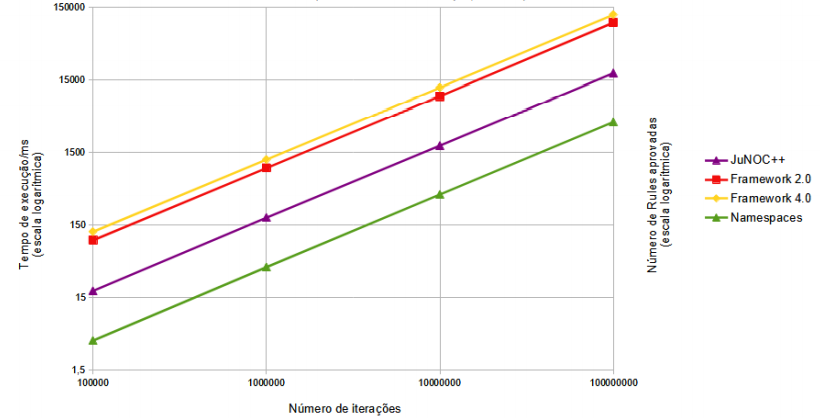
\includegraphics[width=.85\textwidth]{../figures/junoc_graph.png}
  \caption*{Fonte: \citeonline{chierichi_2020}}
  \label{fig:exp_junoc}
\end{figure}

O \textit{Framework} PON C++ 4.0 em JuNOC++ foram desenvolvidos em paralelo,
assim sendo, muitas das melhorias propostas são consideradas em ambos. O JuNOC++
aproveitou principalmente as implementações com \textit{templates} introduzidas
pelo \textit{Framework} PON C++, enquanto este buscou inspiração nas melhorias
introduzidas pelo JuNOC++ para facilitar a programação em alto-nível. Ainda
assim, ambos os \textit{frameworks} possuem propostas diferentes, sendo que o
\textit{Framework} PON C++ 4.0 se preocupa em disponibilizar uma materialização
mais estável, com desenvolvimento orientado a testes, incorporando conceitos de
paralelismo, o JuNOC++ é ainda uma materialização de cunho prototipal,
explorando a flexibilização da construção das entidades, com foco na programação
em alto nível.

\subsubsection{Implementações realizadas com o \textit{Framework} PON C++
  2.0}\label{sec:ex_fw2}

Inicialmente, de modo a possibilitar levantar as deficiências do
\textit{Framework} PON C++ 2.0, apontadas na Seção \ref{sec:problemas}, e servir
também como conhecimento de base para a implementação de um novo
\textit{framework}, foram desenvolvidas aplicações utilizando o
\textit{Framework} PON C++ 2.0. Com o desenvolvimento destas aplicações era
objetivado ganhar experiência no desenvolvimento em aplicações com o PON, em
particular com o \textit{Framework} PON C++ 2.0, de forma a facilitar o
entendimento dos pontos de melhoria a serem implementados. Essas implementações
são descritas com maiores detalhes nas seções seguintes.

\paragraph{Futebol de Robôs}

A primeira aplicação desenvolvida pelo autor deste trabalho utilizando o PON foi
no âmbito de Futebol de Robôs. Esta aplicação foi desenvolvida no contexto da
disciplina de Tópicos Especiais em Engenharia da Computação: Paradigma Orientado
a Notificações, via PPGCA, na UTFPR, durante o terceiro trimestre de 2019
\cite{lima_2020}. Tal implementação inspirou-se em trabalho prévio desenvolvido
por \citeonline{msc_santos_2017}, ainda que esta nova implementação tenha sido a
partir de uma versão mais prototipal do trabalho dele por ser a que se encontrou
disponível. Em tempo, o trabalho foi conjunto entre cinco discentes da
disciplina, sendo que cada qual montou um dado conjunto de \textit{Rules}
subsequentemente integradas \cite{lima_2020}.

Neste âmbito, de forma a aplicar os conhecimentos adquiridos durante a
disciplina foi proposto o desenvolvimento de uma aplicação de controle de robôs
em \textit{Framework} PON C++ 2.0, em contexto de Futebol de Robôs, para
execução em ambiente de simulação. Essa aplicação consiste do controle de duas
equipes, compostas cinco robôs cada, executada em um ambiente virtual que simula
um campo de futebol. Uma tela da execução deste ambiente de simulação é mostrada
na Figura \ref{fig:futebol_robos}, na qual é possível observar o campo e os
robôs de ambos os times.

Nesse cenário, a parte da aplicação desenvolvida em \textit{Framework} PON C++
2.0 é responsável por receber e processar comandos de um juiz virtual que envia
os comados da partida (\textit{e.g.}, início, parada, falta etc.), assim como a
aplicação desenvolvida em \textit{Framework} PON C++ 2.0 é responsável por
controlar de forma autônoma todos os robôs de ambas as equipes. Cada equipe é
controlada por uma instância independente da aplicação em PON \cite{lima_2020}.
Para o desenvolvimento em PON desta aplicação foi utilizado o \textit{Framework}
PON C++ 2.0 conforme o que definido em \citeonline{msc_Ronszcka_2012} e
\citeonline{msc_valenca_2012}. 

\begin{figure}[!htb]
  \centering
  \caption{Tela principal do ambiente de simulação do futebol de robôs}
  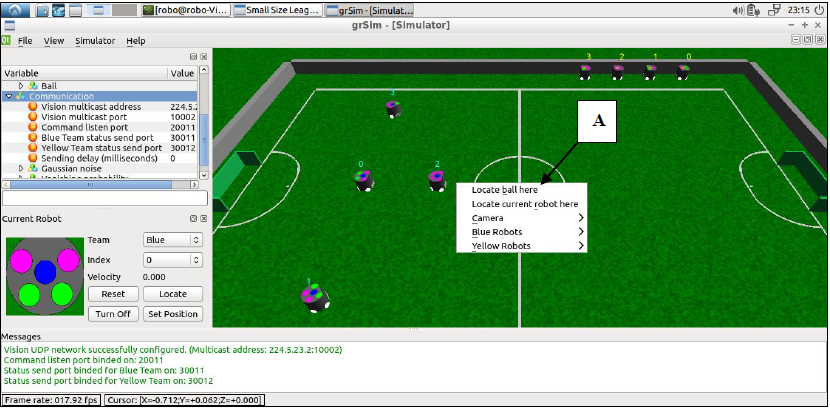
\includegraphics[width=0.95\textwidth]{../figures/futebol_robos.png}
  \smallskip
  \caption*{Fonte: \citeonline{lima_2020}}
  \label{fig:futebol_robos}
\end{figure}

No escopo deste trabalho foi utilizado um ambiente previamente configurado e
funcional, contendo um conjunto básico de \textit{Rules} e \textit{FBEs} já
existentes, fruto de uma versão prototipal dos esforços da dissertação de
mestrado de \citeonline{msc_santos_2017}, conforme já especificado acima.
Baseado nessa estrutura inicial, representada pelo diagrama de classes da Figura
\ref{fig:class_futebol}, foram apenas desenvolvidas novas \textit{Rules},
utilizando os \textit{FBEs} já existentes \textit{RobotPON} e
\textit{StrategyPON}. O artigo-relatório contendo todo o desenvolvimento deste
projeto é apresentado na íntegra no \nameref{ch:apendice_futebol}, para fins de
registro na dissertação.

\begin{figure}[!htb]
    \centering
    \caption{Diagrama de classes do futebol de robôs}
    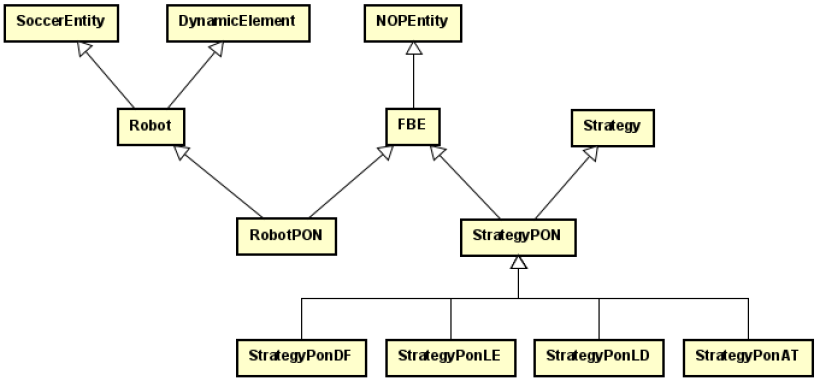
\includegraphics[width=0.7\textwidth]{../figures/class_futebol.png}
    \smallskip
    \caption*{Fonte: \citeonline{lima_2020}}
    \label{fig:class_futebol}
\end{figure}

\FloatBarrier

Durante o desenvolvimento do trabalho foram encontradas algumas dificuldades,
principalmente no que se refere ao uso do ambiente de desenvolvimento proposto.
Isto primeiramente pelo fato do mesmo ser disponibilizado inicialmente na forma
de uma máquina virtual que necessitava se configurada e instalada. Ainda, uma vez
instalada a máquina e o ambiente como um todo, percebeu-se que não continha
todas as \textit{Rules} e, principalmente, não continha \textit{FBEs} com seus
\textit{Methods} e \textit{Attributes} de acordo com a dissertação de
\citeonline{msc_santos_2017}, concluindo-se subsequentemente que se tratava de
um código mais prévio ou prototipal \cite{lima_2020}.

No contexto acima relatado, especialmente devido ao ambiente conter um número de
\textit{FBEs} implementados muito pequeno, não havia recursos para se fazer a
criação das novas \textit{Rules} de forma muito abundante. Ainda, perceberam-se
outros fatores em algo obstantes, como o fato de recursos mais avançados do
\textit{framework}, como \textit{Master Rule} e \textit{SubConditions}, não
possuírem uma construção tão intuitiva quanto seria possível, bem como não haver
instruções de utilização adequadas, o que dificultou a implementação das
\textit{Rules} que foram criadas.

Em função destas dificuldades postas, também percebeu-se a curva não tão suave
(conforme habilidade de cada qual) de aprendizado do \textit{Framework} PON C++
2.0, ao menos neste exemplo em questão. Não obstante as dificuldades, a criação
de conjuntos de \textit{Rules} pelos discentes permitiu bem compreender o PON.
Ademais, também foi possível observar propriedades do PON, como os conjuntos de
\textit{Rules} trabalhando harmonicamente no final da implementação, isto sem
esforços extraordinários de integração em função do nível de desacoplamento
entre eles.

\paragraph{Jogo NOPUnreal}\label{sec:nopunreal}

A segunda aplicação, já desenvolvida após certa familiarização com o
desenvolvimento em PON foi realizada sob a forma de um jogo. A proposta desta
aplicação era realizar a integração do \textit{Framework} PON C++ 2.0 com uma
API complexa de desenvolvimento de jogos. Para este fim foi escolhida a Unreal
Engine. Em tempo, este foi um trabalho desenvolvido no contexto da disciplina de
Estudo Especial — Paradigmas de Programação, via CPGEI, na UTFPR, durante o
primeiro trimestre de 2020 \cite{neves_2020}\footnote{Este trabalho também foi
apresentado sob a forma de minicurso no SICITE 2020}. A estrutura básica do jogo
consiste em uma nave controlada pelo jogador com o objetivo de neutralizar todos
os inimigos. A Figura \ref{fig:jogo_fw2} mostra uma tela do jogo desenvolvido,
na qual o jogador é representado pela nave cinza, e os inimigos pelas naves
amarelas.

\begin{figure}[!htb]
  \centering
  \caption{\textit{Screenshot} do jogo desenvolvido} \includegraphics[width=\textwidth]{../figures/game.png}
  \smallskip
  \caption*{Fonte:
      \citeonline{neves_2020}}
  \label{fig:jogo_fw2}
\end{figure}

A Unreal Engine foi escolhida por ser o motor gráfico mais utilizado no
desenvolvimento de jogos e aplicações gráficas comerciais, chegando a ser
utilizada em cerca de 20\% dos jogos de computador \cite{neves_2020}. O
desenvolvimento desta aplicação foi realizado utilizando tanto com o POO como o
PON, de modo a permitir a comparação da facilidade de programação utilizando os
dois paradigmas. De modo geral o desenvolvimento foi mais fácil e rápido
utilizando o PON, chegando a obter um tempo de desenvolvimento até 38.62\%
menor, porém a verbosidade do \textit{Framework} PON C++ 2.0 resultou em um
código-fonte com 12.16\% mais linhas que a implementação equivalente no POO
\cite{neves_2020}.

Um dos elementos que dificulta a aplicação do PON neste projeto é a rigidez da
estrutura da API da Unreal Engine, sendo implementada utilizando o POO e fazendo
uso extensivo de lógica sequencial na sua execução. Neste contexto, o
desenvolvedor é obrigado a utilizar as estruturas e classes próprias da Unreal
Engine para a sua implementação. Na Figura \ref{fig:class_jogo_fw2}\footnote{Nos
diagramas de classe construídos com a ferramenta PlantUML o símbolo C em um
círculo verde identifica classes concretas, já o símbolo A sobre um círculo azul
identifica classes abstratas} é mostrado o diagrama de classes do jogo
desenvolvido, no qual é importante destacar que as classes implementadas em PON,
derivadas da classe \textit{FBE}, também são derivadas das classes próprias de
Unreal Engine (\textit{APawn}, \textit{AActor}, \textit{UObject},
\textit{UActorComponent} e \textit{AInfo}). Deste modo pode ser dito que o
código implementado é, na verdade, multiparadigma, pois utiliza tanto o PON como
o POO na sua implementação. 

Nesse contexto de programação multiparadigma, o PON
é utilizado para implementar a lógica referente ao comportamento dos inimigos e
às regras do jogo, enquanto o POO é utilizado para a implementação dos elementos
gráficos da aplicação. O artigo-relatório contendo o desenvolvimento deste
projeto, inclusive contendo a especificação completa de todas as \textit{Rules}
implementadas, é apresentado na íntegra no \nameref{ch:apendice_nopunreal}.

A implementação deste projeto realçou algumas das deficiências ou imperfeições
do \textit{Framework} PON C++ 2.0. Um dos principais problemas foi a baixa
flexibilidade de tipos, que fica bem evidente devido à Unreal Engine utilizar
muitos tipos próprios, como estruturas, enumerações e classes (\textit{e.g.}
\textit{FVector}, \textit{FString} etc.).

\begin{figure}[!htb]
  \centering
  \caption{Diagrama de classes do jogo desenvolvido}
  \includegraphics[width=\textwidth]{../out/diagrams/class_diagram_nop/NOPUnreal.png}
  \smallskip
  \caption*{Fonte: \citeonline{neves_2020}}
  \label{fig:class_jogo_fw2}
\end{figure}

O fato do \textit{Framework} PON C++ 2.0 somente permitir o uso de seus tipos
pré-definidos (\textit{int}, \textit{double}, \textit{bool} e \textit{string})
faz com que seja necessário converter os tipos próprios da Unreal Engine para a
utilização em conjunto com as entidades do PON. Alguns exemplos que melhor
ilustram esse problema são apresentados abaixo. No Código
\ref{cod:integer_cast}, um \textit{Attribute} do tipo \textit{int} é utilizado
para implementar um tipo que utiliza uma enumeração, exigindo que seja realizada
uma conversão de tipos.

\begin{lstlisting}[caption = {Uso de \textit{static\_cast} para converter enumerações}, float=htb,
source = {Autoria própria},
label = {cod:integer_cast}]
INTEGER(this, atStrategym static_cast<int>(ENOPEnemyStrategy:EFollow));
\end{lstlisting}

Por sua vez, também o Código \ref{cod:fvector} mostra a estrutura FVector, muito
utilizada em todo o código para representar a posição no espaço tridimensional
dos objetos. Porém, o uso dela em \textit{Premises} e \textit{Attributes} é
impossível, pois não é um tipo básico suportado. Assim, faz necessários
desmembramentos e afins para seu uso. 

\begin{lstlisting}[caption = {Estrutura \textit{FVector} da Unreal Engine}, float=htb,
source = {Autoria própria},
label = {cod:fvector}]
struct FVector {
    float X;
    float Y;
    float Z;
}
\end{lstlisting}

Por fim, o Código \ref{cod:flexibilidade_pon} apresenta uma situação na qual é
necessário criar \textit{Premises} muito semelhantes, porém, com avaliações
opostas. Devido à baixa flexibilidade algorítmica não permitir a criação de
\textit{Conditions} com composição de \textit{Premises} utilizando declaração de
operações lógicas mais diversas sobre elas, como seria o caso de uma operação de
negação, ocorre este tipo de redundância estrutural.

\begin{lstlisting}[caption = {Uso de premissas redundantes no PON}, float=htb,
source = {Autoria própria},
label = {cod:flexibilidade_pon}]
PREMISE(prIsFarFromTarget, atDistanceToTarget, 800.0f, Premise::GREATEROREQUAL, Premise::STANDARD, false);
PREMISE(prIsNOTFarFromTarget, atDistanceToTarget, 800.0f, Premise::SMALLERTHAN, Premise::STANDARD, false);
\end{lstlisting}

Em suma, o desenvolvimento de ambas estas aplicações permitiu principalmente
observar as limitações do \textit{Framework} PON C++ 2.0, explorados em detalhes
na Seção \ref{sec:problemas}. Ainda, essas experiências serviram também como
fator motivador para a proposta do \textit{Framework} PON C++ 4.0.

\subsubsection{Considerações sobre os \textit{frameworks} do PON em C++}

De forma geral, as materializações do PON por meio de \textit{frameworks} em
linguagem de programação C++ representam uma grande contribuição ao estado da
técnica do PON, possibilitando o desenvolvimento de aplicações que permitiram
avaliar e comparar o desempenho do PON
\cite{msc_Banaszewski_2009,msc_Ronszcka_2012,msc_valenca_2012}. Nas
materializações de \textit{frameworks} em C++, foram desenvolvidas a maior parte
das aplicações feitas em PON conforme
\cite{msc_Ronszcka_2012,msc_santos_2017,doc_ronszcka_2019}.

Houve também o desenvolvimento de diversas aplicações como os
\textit{frameworks} do PON em C++, nomeadamente a aplicação Mira ao Alvo
\cite{msc_Banaszewski_2009,msc_Ronszcka_2012,msc_valenca_2012}, o Futebol de
Robôs \cite{msc_santos_2017,lima_2020}, o jogo NOPUnreal \cite{neves_2020} e
também o NeuroPON \cite{belmonte_2012,belmonte_2016,doc_Schutz_2019}. Todas
estas aplicações desenvolvidas são interessantes em pertinentes, demonstrando
diversos casos de uso do PON, assim como servindo de \textit{benchmarks}, como o
caso da aplicação Mira ao Alvo (que posteriormente evoluí sob nova forma de rede
de sensores), frequentemente utilizada para comparações de desempenho entre os
\textit{frameworks}. 

Apesar disso, essas aplicações têm utilização limitada ao contexto do grupo de
pesquisa do PON, de forma que estes \textit{frameworks} carecem de
\textit{benchmarks} universalizados, mais conhecidos pela comunidade científica.
Salienta-se inclusive que aplicações como o Futebol de Robôs não são
particularmente adequadas para fins \textit{benchmark} em si, por ser uma
aplicação que não se interessa em tempos de execução.

\subsection{\textit{Frameworks} PON Java/C\# 1.0}\label{sec:csharp_java}

Não obstante, além das materializações em C++, também houve a materialização na
forma de \textit{framework} nas linguagens Java e C\#, ainda que assaz
prototipais ou ao menos ainda não utilizadas largamente. Esta seção trata de
forma unificada destas duas materializações em linguagens diferentes, pois as
mesmas são materializações equivalentes principalmente ao \textit{Framework} PON
C++ 1.0 e sob a forma de adaptações dele para tais linguagens
\cite{henzen_2015}.

O objetivo destas materializações foi adaptar o \textit{Framework} PON C++ 1.0
para Java e C\# utilizando técnicas de programação semelhantes, que padronizam e
facilitam a manutenção do código. Estas materializações se justificam pelo
grande número de programadores que utilizam as linguagens Java e C\#, sendo
muito utilizadas, principalmente, em aplicações móveis e web \cite{henzen_2015}.
A linguagem Java também é adotada como principal linguagem no ensino de
programação em diversas universidades, o que contribui para o grande número de
programadores utilizando a mesma \cite{henzen_2015}.

 Para a comparação dos resultados entre as materializações de C++, Java e C\#
foi desenvolvida uma aplicação para controle de um portão eletrônico. A
implementação desta aplicação consiste na criação de duas \textit{Rules}, uma
para abrir e outra para fechar o portão, com base nos \textit{FBEs} do portão,
que encapsula o estado do portão (aberto ou fechado), e controle remoto, que
encapsula o estado do botão (pressionado ou não) \cite{henzen_2015}. As
particularidades das implementações em cada uma das linguagens são apresentadas
nas seções seguintes.


\subsubsection{\textit{Framework} PON Java 1.0}\label{sec:java}

Algumas alterações foram necessárias para implementar o \textit{framework} em
Java, como o fato de a linguagem Java não possuir o conceito herança múltipla,
para isto sendo utilizado como alternativa o conceito de \textit{Interface}. Um
trecho da aplicação desenvolvida com o \textit{Framework} PON Java 1.0 é
apresentado no Código \ref{cod:java_nop}.

\begin{lstlisting}[caption = {Exemplo de \textit{Rule} do portão eletrônico em Java},
source = {Adaptado de \citeonline{henzen_2015}},
label = {cod:java_nop}]

Condition cond1R01 = new Condition(Condition.CONJUNCTION);
cond1R01.addPremise(new Premise(remoteControl.atRemoteControlStatus, NBoolean.TRUE_NOP, Premise.EQUAL, false));
SubCondition subcond1R01 = new SubCondition(SubCondition.DISJUNCTION, false);
subcond1R01.addPremise(new Premise(gate.atGateStatus, 0, Premise.EQUAL, false));
subcond1R01.addPremise(new Premise(gate.atGateStatus, 5, Premise.EQUAL, false));
cond1R01.addSubCondition(subcond1R01);

Action actR01 = new Action();
actR01.addInstigation(new Instigation(gate.mtOpening));
actR01.addInstigation(instStatusOff);

Rule rule1 = new Rule("Opening gate", scheduler, cond1R01, actR01, false);
\end{lstlisting}

\subsubsection{\textit{Framework} PON C\# 1.0}\label{sec:csharp}

Por sua vez, na implementação de \textit{framework} com a linguagem C\# foi
utilizado conceito de \textit{Delegate} no lugar de ponteiros para funções
\cite{henzen_2015}. Um trecho da aplicação desenvolvida com o \textit{Framework}
PON C\# 1.0 é apresentado no Código \ref{cod:csharp}.

\begin{lstlisting}[caption = {Exemplo de \textit{Rule} do portão eletrônico em C\#},
source = {Adaptado de \citeonline{henzen_2015}},
label = {cod:csharp}]
Condition cond1 = new Condition(Condition.CONJUNCTION);
cond1.addPremise(new Premise(remoteControl.bIsPressed,NBoolean.TRUE_NOP,Premise.EQUAL,false));
cond1.addPremise(new Premise(gate.GateStatus,true,Premise.EQUAL,false));

Action action1 = new Action();
action1.addInstigation(new Instigation(remoteControl.bIsPressed,false));
action1.addInstigation(new Instigation(gate.mtOpenGate));

Rule rule1 = new Rule("Open gate", scheduler, cond1, action1, false);
\end{lstlisting}

\subsubsection{Comparações}

Foram realizados testes com 10.000, 100.000, 20.0000 e 500.000 iterações de
fechamento do portão\footnote{Para este teste foi utilizado um computador modelo
Apple Macbook Pro, Core i5 2.5 Ghz, 6 GB de memória RAM, com o sistema
operacional Windows 10 Preview.}, com os resultados mostrados na Figura
\ref{fig:comp_henzen}. O desempenho dos \textit{frameworks} em Java e C\# foi
satisfatório, inclusive superando o desempenho do \textit{Framework} PON C++ 1.0
neste cenário, sendo o \textit{framework} Java aquele que apresentou o melhor
desempenho. Entretanto, seriam necessários mais experimentos para avaliar como
ficariam esses desempenhos, inclusive em relação ao \textit{Framework} PON C++
2.0.

\begin{figure}[!htb]
  \centering
  \caption{Comparação de desempenho das aplicações em C++, Java e C\#}
  \includegraphics[width=.5\textwidth]{../figures/comp_henzen.png}
  \caption*{Fonte: \citeonline{henzen_2015}}
  \label{fig:comp_henzen}
\end{figure}

Isto dito, o desenvolvimento destes \textit{frameworks} demonstrou ser possível
a implementação de um \textit{framework} do PON em Java e C\#, inspirado no
\textit{Framework} PON C++ 1.0, sem haver descaracterização das técnicas
empregadas na implementação original \cite{henzen_2015}. Apesar do aspecto
prototipal destes \textit{frameworks}, seu desenvolvimento abriu novos caminhos
de pesquisa para o PON explorando tais plataformas, como o subsequente
desenvolvimento do \textit{Framework} PON C\# IoT.

\FloatBarrier

\subsection{\textit{Framework} PON C\# IoT}

Na materialização \textit{Framework} PON C\# IoT, desenvolvida à luz dos
esforços de \citeonline{msc_oliveira_2019} introduzem uma versão com o foco em
Internet das Coisas (IoT - \textit{Internet of Things}). Do ponto de vista de
implementação esta versão se inspira no \textit{framework} PON C++ 2.0 e
adapta/evolui o \textit{Framework} PON C\# 1.0, com o seu diferencial sendo a
proposta da distribuição em rede das entidades do PON, permitindo a aplicação
dos conceitos de IoT, por meio de paralelismo, distribuição e a capacidade de
reconfiguração das \textit{Rules} em tempo de execução \cite{msc_oliveira_2019}.

A Figura \ref{fig:classes_pon_iot} apresenta o diagrama de classes do
\textit{Framework} PON C\# IoT. Apesar de apresentar uma estrutura bastante
similar ao \textit{Framework} PON C++ 2.0 e C\# 1.0 também é possível observar
neste diagrama a adição de classes específicas para aplicação no ambiente
distribuído, como a classes \textit{SensorFBE} e \textit{NotificationNetwork}.

\begin{figure}[!htb]
  \centering
  \caption{Diagrama simplificado de classes do \textit{Framework} PON C\# IoT}
  \includegraphics[width=\textwidth]{../figures/classes_pon_iot.png}
  \caption*{Fonte: \citeonline{msc_oliveira_2019}}
  \label{fig:classes_pon_iot}
\end{figure}

Este \textit{Framework} PON C\# IoT utiliza uma unificação das entidades
\textit{FBE} e \textit{Attribute}, chamada de \textit{SensorFBE}, na qual o
\textit{FBE} possui apenas um único \textit{Attribute}, relativo a leituras do
sensor ou atuador. O \textit{SensorFBE} também possui alguns outros atributos
não relativos ao mecanismo de notificações do PON, como identificador único,
nome, tipo, intervalo de leitura, e outras definições relativas ao
sensor/atuador\footnote{Este \textit{framework} foi projetado para trabalhar com
uma placa RaspberryPi, portanto apresenta configurações específicas para lidar
diretamente com as entradas e saídas desta placa} \cite{msc_oliveira_2019}. A
entidade \textit{SensorFBE} ainda possui outras variáveis que controlam a forma
de notificação das \textit{Premises}, como o controle de notificação, podendo
ser \textit{Always}, \textit{On change} ou \textit{Never}. As entidades
\textit{SensorFBE} podem ser executadas de forma distribuída, sendo capazes de
notificarem \textit{Premises} sendo executadas em outros dispositivos remotos.

O processo de notificação é executado de forma paralela, utilizando a função
\textit{Parallel.ForEach} do C\#, de modo que cada notificação gerada pelo
\textit{SensorFBE} é processada em uma \textit{thread} diferente
\cite{msc_oliveira_2019}. Ainda, nas situações nas quais a entidade a ser
notificada pode estar em um ambiente remoto, como em outro dispositivo, a
notificação é enviada utilizando o mecanismo que permite o envio para outros
clientes, o \textit{IoT.NotificationClient.Notification}, com o uso do método
\textit{Send}. Deste modo a notificação é enviada para os outros dispositivos
via protocolo TCP/IP \cite{msc_oliveira_2019}. A Figura \ref{fig:ativ_pon_iot}
ilustra as atividades executadas durante o processo de leitura de um sensor
físico utilizando o \textit{Framework} PON C\# IoT.

\begin{figure}[!htb]
  \centering
  \caption{Diagrama de atividades do PON C\# IoT}
  \includegraphics[width=0.9\textwidth]{../figures/pon_iot_flow.png}
  \caption*{Fonte: \citeonline{msc_oliveira_2019}}
  \label{fig:ativ_pon_iot}
\end{figure}

O \textit{Framework} PON C\# IoT também faz o uso do conceito de impertinência
dinâmica de \textit{Attributes} e \textit{Premises}. Neste mecanismo, sem a
interferência do desenvolvedor, a própria \textit{Condition} define a
impertinência de suas \textit{Premises}, baseado no valor lógico das outras
\textit{Premises} e estas de seus respectivos \textit{Attibutes}, baseado na
relevância de cada \textit{Premise} na aprovação da \textit{Condition}. Por
exemplo, no caso de uma \textit{Condition} com operação lógica de conjunção, as
demais \textit{Premises} somente tem suas notificações ativadas após a primeira
\textit{Premise} definida como mais relevante possuir valor lógico verdadeiro
\cite{msc_oliveira_2019}. 

Esse \textit{framework} foi aplicado para o desenvolvimento do NOCS
(\textit{Notification Oriented Care System}), com a utilização do ambiente
distribuído mostrado na Figura \ref{fig:pon_iot}, por meio da conexão dos
sensores e atuadores utilizando a entidade \textit{SensorFBE} em um dispositivo
RaspberryPi remoto (NOCS Control), que se comunica com um servidor central (NOCS
Server), capaz de executar os processos de interface com o usuário e comunicação
com outros dispositivos \cite{msc_oliveira_2019}. 

\begin{figure}[!htb]
  \centering
  \caption{Diagrama de componentes PON C\# IoT}
  \includegraphics[width=.55\textwidth]{../figures/pon_iot.png}
  \caption*{Fonte: \citeonline{msc_oliveira_2019}}
  \label{fig:pon_iot}
\end{figure}

Ainda, o NOCS Server disponibiliza uma interface web na qual os usuários podem
visualizar os estados dos sensores/atuadores, assim como criar \textit{Rules} em
tempo de execução da aplicação. Ademais, utilizando a mesma API é possível acessar
estes mesmos dados por meio de um aplicativo (NOCS Mobile). Além disso, também é
possível a utilização de um simulador de ambiente que simula os sensores e
atuadores que estariam normalmente conectados no NOCS Control
\cite{msc_oliveira_2019}. Nesta aplicação as \textit{Rules} eram criadas de forma
dinâmica utilizando a interface do NOCS Server, ainda assim o Código
\ref{cod:rule_iot} mostra um exemplo de construção estática de uma \textit{Rule}
para controle de temperatura pertinente a esta aplicação.

\begin{lstlisting}[caption = {Exemplo de \textit{Rule} com o \textit{Framework} PON C\# IoT},
  source = {Adaptado de \citeonline{msc_oliveira_2019}}, float=htb,
  label = {cod:rule_iot}]
SensorFBE sensor1 = new SensorFBE(1, "Thermometer1", "", 0, "", "", 
                      DistributedNotification, NotificationControl.OnChange);
SensorFBE sensor2 = new SensorFBE(2, "Thermometer2", "", 0, "", "",
                      DistributedNotification, NotificationControl.OnChange);
SensorFBE sensor3 = new SensorFBE(3, "Thermometer3", "", 0, "", "", 
                      DistributedNotification, NotificationControl.OnChange);
SensorFBE sensor4 = new SensorFBE(4, "Air1", "", 0, "", "", 
                      DistributedNotificationType.Rest, NotificationControl.OnChange);

Rule rule1 = new Rule(1, "TempControl1", 0);
var subcondition1 = rule1.Condition.AddSubCondition(1);
subcondition1.LogicalOperator = Library.LogicalOperator.Disjunction;
subcondition1.AddPremisse(1, sensor1, "Thermometer1 > 20");
subcondition1.AddPremisse(1, sensor2, "Thermometer2 > 20");
subcondition1.AddPremisse(1, sensor3, "Thermometer3 > 20");
var subcondition2 = rule1.Condition.AddSubCondition(1);
subcondition2.AddPremisse(1, sensor4, "Air1 = 0");
Method method1 = new Method(1, sensor4, 1);
var instigarion1 = rule1.Action.AddInstigationSequential(1, "");
instigarion1.AddMethodSequential(method1);
Method method2 = new Method(1, sensor7, 1);
instigarion1.AddMethodSequential(method2);
\end{lstlisting}

Na Figura \ref{fig:teste_pon_iot} é apresentado um resultado de teste de
\textit{stress} do monitoramento de ambientes utilizando RaspberryPi. Nesse
teste, coletou-se o número de leituras dos sensores, avaliações de
\textit{Premises} e o tempo total de execução, obtendo uma média de 235
notificações de sensores por segundo, e a média de 415 avaliações de
\textit{Premises} por segundo, totalizando uma média de 650 execuções por
segundo \citeonline{msc_oliveira_2019}. Esses testes permitiram mensurar, neste
cenário específico, o número máximo de notificações que o sistema consegue
processar por segundo.

\begin{figure}[!htb]
  \centering
  \caption{Resultados de testes do PON C\# IoT}
  \includegraphics[width=.75\textwidth]{../figures/teste_pon_iot.png}
  \caption*{Fonte: \citeonline{msc_oliveira_2019}}
  \label{fig:teste_pon_iot}
\end{figure}

\subsection{\textit{Framework} PON Elixir/Erlang}

Esta materialização chamada \textit{Framework} PON Elixir/Erlang é fruto dos
esforços de mestrado de \citeonline{msc_negrini_2019}, sendo proposta com o
objetivo de aproveitar os conceitos de desacoplamento e, portanto, potencial
paralelização das entidades do PON em conjunto ao modelo de atores da
arquitetura Erlang \cite{msc_negrini_2019}.

Em termos de paradigma, a linguagem Elixir/Erlang segue os princípios do
Paradigma Funcional (PF) associado com o Paradigma Orientado a Atores (POA).
Nesta materialização é introduzido uma implementação na qual os elementos do PON
são modelados por meio de atores. O modelo de atores pode ser definido como uma
extensão dos modelos modulares declarativos ou imperativos, com a passagem
assíncrona de mensagens entre os agentes computacionais elaborados
declarativamente \cite{msc_negrini_2019}.

No \textit{Framework} PON Elixir/Erlang, tanto os elementos da base de fatos
(\textit{i.e.}, \textit{FBEs}, \textit{Attributes} e \textit{Methods}), quanto
suas condições lógico-causais (\textit{i.e.},\textit{Rules},
\textit{Conditions}, \textit{Premises}) e ativadores
(\textit{i.e.},\textit{Actions} e \textit{Instigations}) são desmembrados em
vários atores, enquanto as notificações são implementadas por meio de mensagens
assíncronas, de modo que cada ator carrega uma pequena parte do fluxo de
processamento, cunhando assim micro-atores \cite{msc_negrini_2019}. Um
detalhamento dessa implementação é apresentado por meio da modelagem em UML
apresentada na Figura \ref{fig:pon_elixir_uml}.

\begin{figure}[!htb]
  \centering
  \caption{Modelagem UML dos elementos do PON enquanto mircro-atores}
  \includegraphics[width=0.9\textwidth]{../figures/pon_elixir_uml.png}
  \smallskip
  \caption*{Fonte: \citeonline{msc_negrini_2019}}
  \label{fig:pon_elixir_uml}
\end{figure}
\FloatBarrier

A utilização do \textit{Framework} PON Elixir/Erlang é exemplificada por meio da
implementação de um conjunto de \textit{FBE} e \textit{Rule} bastante simples,
conforme descrito no Código \ref{cod:fbe_negrini}, e implementado com o
\textit{framework} no Código \ref{cod:negrini_rule}. Neste exemplo é descrito um
\textit{FBE} com apenas um \textit{Attribute} \textit{atValue}, e uma
\textit{Rule} que altera o seu valor para 3 quando seu valor é 5, conforme a
\textit{Condition} descrita. Esse exemplo ilustra a utilização da especialização
de \textit{NOP.Element.FBE} e \textit{NOP.Element.Rule} para a implementação das
entidades do PON.

\begin{lstlisting}[language=C++, caption={Exemplo descrito em \textit{FBE} e \textit{Rule}},
label = {cod:fbe_negrini}, float=htb,
source = {Fonte: Autoria própria}
]
fbe Dummy
  public integer atValue = 0
  private method change_value_to_3
    attribution
      this.atValue = 3
    end_attribution
  end_method
  rule rlExample
    condition
      premise prExample
        this.atValue == 5
      end_premise
    end_condition
    action sequential
      instigation sequential
        call this.change_value_to_3()
      end_instigation
    end_action
  end_rule
end_fbe
\end{lstlisting}

\begin{lstlisting}[language = elixir, caption = {Exemplo de implementação de \textit{Rule} como especialização de \textit{NOP.Element.Rule}}, %float=htb,
    source = {Adaptado de \citeonline{msc_negrini_2019}}, label = {cod:negrini_rule}, float=htb]
defmodule NOP.Element.FBE_dummy do
  use NOP.Element.FBE

  defp int_attribuges() do
    %{:value => 0}
  end

  def change_value_to_3(fbe) do
    NOP.Service.FBE.set_attribute(fbe, :value, 3)
  end
end

defmodule NOP.Element.Rule_example do
  use NOP.Element.Rule

  defp create_element_list([fbe]) do
    premise = NOP.Service.Premise.create_premise(
      "NOP.element.premise", fbe, :value, :EQ, 5)
    [premise]
  end

  defp create_instigation_list([fbe]) do
    [{NOP.Element.FBE_dummy, :change_value_to_3, [fbe]}]
  end

end
\end{lstlisting}
\FloatBarrier

Para a validação deste \textit{framework} foi escolhida uma aplicação de
Controle de Tráfego Automatizado (CTA)\footnote{Maiores detalhes sobre esta
aplicação podem ser encontrados em \cite{renaux_2015}}. O objetivo do CTA é
simular o tráfego de uma área urbana e aplicar diferentes estratégias de
controle automatizado de tráfego, de modo a avaliar o desempenho computacional
conforme a estratégia \cite{msc_negrini_2019}. Os testes foram realizados com o
objetivo de avaliar a carga nos núcleos do processador em diferentes ambientes,
com 2, 4, 8 e 16 núcleos. Esses ambientes são identificados na Figura
\ref{fig:ambientes_elixir}.

\begin{figure}[!htb]
  \centering
  \caption{Detalhamento dos ambientes do experimento do \textit{Framework} PON
    Elixir/Erlang} \includegraphics[width=0.65\textwidth]{../figures/maquinas_elixir.png}
  \smallskip
  \caption*{Fonte: \citeonline{msc_negrini_2019}}
  \label{fig:ambientes_elixir}
\end{figure}

As Figuras \ref{fig:vm02}, \ref{fig:vm04}, \ref{fig:vm08} e \ref{fig:vm16}
exibem a taxa média de ocupação por núcleo e tempo total de execução do
experimento para cada um dos ambientes. Estes resultados apresentam uma
expressiva redução do tempo de execução conforme são acrescidos núcleos aos
ambientes, bem como apresentam que a taxa de ocupação dos núcleos se manteve
balanceada durante a simulação, demonstrando que a execução lógico-causal foi
distribuída com um bom nível de balanceamento entre os núcleos
\cite{msc_negrini_2019}.

\begin{figure}[!htb]
  \centering
  \begin{minipage}{.5\textwidth}
    \centering
    \captionof{figure}{Taxa média de ocupação por núcleo em ambiente VM02}
    \includegraphics[width=\linewidth]{../figures/vm02.png}
    \captionof{figure}*{Fonte: \citeonline{msc_negrini_2019}}
    \label{fig:vm02}
  \end{minipage}%
  \begin{minipage}{.5\textwidth}
    \centering
    \captionof{figure}{Taxa média de ocupação por núcleo em ambiente VM02}
    \includegraphics[width=\linewidth]{../figures/vm04.png}
    \captionof{figure}*{Fonte: \citeonline{msc_negrini_2019}}
    \label{fig:vm04}
  \end{minipage}
\end{figure}

\begin{figure}[!htb]
  \centering
  \begin{minipage}{.5\textwidth}
    \centering
    \captionof{figure}{Taxa média de ocupação por núcleo em ambiente VM08}
    \includegraphics[width=\linewidth]{../figures/vm08.png}
    \captionof{figure}*{Fonte: \citeonline{msc_negrini_2019}}
    \label{fig:vm08}
  \end{minipage}%
  \begin{minipage}{.5\textwidth}
    \centering
    \captionof{figure}{Taxa média de ocupação por núcleo em ambiente VM16}
    \includegraphics[width=\linewidth]{../figures/vm16.png}
    \captionof{figure}*{Fonte: \citeonline{msc_negrini_2019}}
    \label{fig:vm16}
  \end{minipage}
\end{figure}

\FloatBarrier

\citeonline{doc_Schutz_2019} também utilizou o \textit{Framework} PON
Elixir/Erlang para a execução da RNA MLP para a função XOR em NeuroPON. Para
isto o código foi desenvolvido espelhando-se no experimento realizado com o
\textit{Framework} PON C++ 3.0. A aplicação desenvolvida foi executada em quatro
ambientes diferentes, com 1, 2, 4 e 8 \textit{cores} cada respectivamente.
Conforme os resultados apresentados na Figura \ref{fig:neuropon_elixir},
observa-se que a execução no ambiente com \textit{octa core} apresenta uma
redução de 94\% no tempo de execução quando comparado ao ambiente \textit{mono
core}. 

\begin{figure}[!htb]
  \centering
  \smallskip
  \caption{Tempos médios de execução NeuroPON de uma RNA MLP para a função XOR
  no \textit{Framework} PON Elixir/Erlang}
  \includegraphics[width=0.8\textwidth]{../figures/neuropon_elixir.png}
    \smallskip
    \caption*{Fonte:
  \citeonline{doc_Schutz_2019}}
  \label{fig:neuropon_elixir}
\end{figure}

Isto posto, é possível afirmar que o \textit{Framework} PON Elixir/Erlang é de
grande valia para a execução da NeuroPON, obtendo resultados muito superiores
(em termos de benefícios da paralelização) aos obtidos com a mesma aplicação no
\textit{Framework} PON C++ 3.0. Esse resultado é devido à maneira como o
paralelismo intrínseco ao modelo de atores da linguagem de programação
Elixir/Erlang e implementado por meio do \textit{Framework} PON Elixir/Erlang é
mais eficiente do que o implementado com o \textit{Framework} PON C++ 3.0. Por
fim, esse experimento permite melhor perceber a valia de NeuroPON já em termos
de paralelismo em software \cite{doc_Schutz_2019}.

\subsection{\textit{Framework} PON Akka.NET}\label{sec:akka}

Outro \textit{framework} implementado utilizando o modelo de atores, como
utilizado no \textit{Framework} Elixir/Erlang, mas de maneira um tanto mais
prototipal, é o \textit{Framework} PON Akka.NET, no qual o trabalho das
entidades do PON é distribuído em atores. A Figura \ref{fig:akka_actor} ilustra
a estrutura do modelo de atores em Akka.NET. Os atores criados pela aplicação
são criados sobre o endereço \textit{/root/user}, enquanto os atores criados
automaticamente pelo sistema são criados em \textit{/root/system}. Todos os
atores são acessíveis por seu endereço, mesmo em sistemas distribuídos
\cite{martini_2019}.

\begin{figure}[!htb]
  \centering
  \caption{Estrutura de atores em Akka.NET}
  \includegraphics[width=0.9\textwidth]{../figures/atores_akka.png}
  \smallskip
  \caption*{Fonte: \citeonline{martini_2019}}
  \label{fig:akka_actor}
\end{figure}

Os atores se comunicam entre si por meio de um sistema de mensagens. Cada ator
possui uma referência aos atores que precisam receber suas mensagens. As
notificações do PON são implementadas por meio deste mecanismo de mensagens
\cite{martini_2019}. A mesma aplicação do portão eletrônico, descrita em
detalhes na Seção \ref{sec:csharp_java}, foi desenvolvida com este \textit{framework}.
O diagrama do modelo de atores para esta aplicação é mostrado na Figura
\ref{fig:akka_portao}.

\begin{figure}[!htb]
  \centering
  \caption{Modelo de atores na aplicação do portão eletrônico em Akka.NET}
  \includegraphics[width=0.9\textwidth]{../figures/akka_actor.png}
  \smallskip
  \caption*{Fonte: \citeonline{martini_2019}}
  \label{fig:akka_portao}
\end{figure}

Ainda em termos de códigos, em um momento posterior, aquelas entidades criadas,
conforme ilustrado no Código \ref{cod:akka_create}, precisam ser conectadas de
forma a passar as referências para o processo de envio de mensagens do Akka.NET,
sendo tal processo ilustrado no Código \ref{cod:akka_link}.

\begin{lstlisting}[language = csh, caption = {Criação de atores em Akka.NET}, %float=htb,
source = {Adaptado de \citeonline{martini_2019}}, label = {cod:akka_create}, language={csh}]
IActorRef FBEGateActor = NOPActorSystem.ActorOf(Props.Create(() ->
    new FBEGate()), "FBEGateActor");
IActorRef FBERemoteControlActor = NOPActorSystem.ActorOf(Props.Create(() ->
    new FBERemoteControl()), "FBERemoteControlActor");
IActorRef PremisseIsClosedActor = NOPActorSystem.ActorOf(Props.Create(() ->
    new PremisseIsClosed()), "PremisseIsClosedActor");
IActorRef PremisseIsOpenActor = NOPActorSystem.ActorOf(Props.Create(() ->
    new PremisseIsOpen()), "PremisseIsOpenActor");
IActorRef PremiseChangeStateActor = NOPActorSystem.ActorOf(Props.Create(() ->
    new PremiseChangeState()), "PremiseChangeStateActor");
IActorRef ConditionCloseGateActor = NOPActorSystem.ActorOf(Props.Create(() ->
    new ConditionCloseGate()), "ConditionCloseGateActor");
IActorRef ConditionOpenGateActor = NOPActorSystem.ActorOf(Props.Create(() ->
    new ConditionOpenGate()), "ConditionOpenGateActor");
IActorRef ConditionSateChangedActor = NOPActorSystem.ActorOf(Props.Create(() ->
    new ConditionSateChanged()), "ConditionSateChangedActor");
\end{lstlisting}

\begin{lstlisting}[language = csh, caption = {Conexão entre atores em Akka.NET}, %float=htb,
source = {Adaptado de \citeonline{martini_2019}}, label = {cod:akka_link}, language={csh}]
var FBEGateActorTask1 = FBEGateActor.Ask(
    new ActorReference(ActorRefType.PremisseIsClosedRef, PremisseIsClosedActor));
var FBEGateActorTask2 = FBEGateActor.Ask(
    new ActorReference(ActorRefType.PremisseIsOpenRef, PremisseIsOpenRefActor));
var FBERemoteControlActorTask1 = FBERemoteControlActor.Ask(
    new ActorReference(ActorRefType.PremisseChangeStateRef, PremisseChangeStateActor));
var PremisseIsOpenActorTask1 = PremisseIsOpenActor.Ask(
    new ActorReference(ActorRefType.ConditionCloseGateRef, ConditionCloseGateActor));
var PremisseChangeStateActorTask1 = PremiseChangeStateActor.Ask(
    new ActorReference(ActorRefType.ConditionOpenGateRef, ConditionOpenGateActor));
var PremisseChangeStateActorTask2 = PremiseChangeStateActor.Ask(
    new ActorReference(ActorRefType.ConditionCloseGateRef, ConditionCloseGateActor));
var PremisseChangeStateActorTask3 = PremiseChangeStateActor.Ask(
    new ActorReference(ActorRefType.ConditionOpenGateRef, ConditionOpenGateActor));
var ConditionCloseGateActorTask1 = ConditionCloseGateActor.Ask(
    new ActorReference(ActorRefType.FBEGateRef, FBEGateActor));
var ConditionCloseGateActorTask2 = ConditionCloseGateActor.Ask(
    new ActorReference(ActorRefType.FBERemoteControlRef, FBERemoteControlActor));
var ConditionOpenGateActorTask1 = ConditionOpenGateActor.Ask(
    new ActorReference(ActorRefType.FBEGateRef, FBEGateActor));
var ConditionOpenGateActorTask2 = ConditionOpenGateActor.Ask(
    new ActorReference(ActorRefType.FBERemoteControlRef, FBERemoteControlActor));
var ConditionStateChangedActorTask1 = ConditionStateChangedActor.Ask(
    new ActorReference(ActorRefType.FBERemoteControlRef, FBERemoteControlActor));
\end{lstlisting}

O desempenho deste \textit{framework} é analisado comparando com a aplicação
utilizando o \textit{Framework} PON C++ 3.0. Os resultados da Figura
\ref{fig:result_akka} mostram que com menos atores o desempenho é inferior.
Problemas de alocação de memória do \textit{Framework} PON C++ 3.0 limitaram o
teste a um máximo de 7200 atores, não permitindo uma comparação com um maior
número de atores, no qual o \textit{Framework} Akka.NET tenderia a apresentar
resultados melhores \cite{martini_2019}.

\begin{figure}[!htb]
  \centering
  \caption{Comparação entre o \textit{Framework} PON Akka.NET e C++ 3.0}
  \includegraphics[width=0.8\textwidth]{../figures/result_akka.png}
  \smallskip
  \caption*{Fonte: \citeonline{martini_2019}}
  \label{fig:result_akka}
\end{figure}

\FloatBarrier

\subsection{Reflexões sobre os \textit{frameworks} do PON}\label{sec:reflex}

Esta subseção traz um arrazoado sobre os \textit{frameworks} do PON para
\textit{software} apresentados nas subseções anteriores. Tal arrazoado analisa
estas materializações sobre distintos pontos de vista, nas suas três subseções
que seguem.

\subsubsection{\textit{Frameworks} do PON vis-à-vis sua teoria}

O grande número de materializações disponíveis do PON é interessante, pois
permite a aplicação do PON em diversos ambientes diferentes. Entretanto, cada
uma dessas materializações contempla apenas alguns dos conceitos e propriedades
do PON introduzidos em seções prévias deste presente capítulo.

Os conceitos e o potencial de propriedades que são implementados em cada uma
destas materializações são apresentados nos quadros abaixo. O Quadro
\ref{tab:elementares} relaciona quais propriedades elementares alcançam seus
potenciais, abordadas na Seção \ref{sec:estado_arte_pon}, são contempladas em
cada uma das materializações do PON, do mesmo modo que o Quadro
\ref{tab:conceitos} relaciona os conceitos apresentados na Seção
\ref{sec:conceitos_pon}. 

\begin{tabframed}[!htb]
  \centering
  \caption{Propriedades elementares contempladas nas materializações do PON}
  \smallskip
  \begin{threeparttable}
    \begin{tabularx}{\textwidth}{|l||*{8}{X|}}\hline
      \diagbox{Potencial\\ de propriedade}{Materialização} & 
      Fw. C++ Prot. & Fw. C++ 1.0 & Fw. C++ 2.0 & Fw. C++ 3.0 & Fw. Java /C\# & Fw. C\# IoT & Fw. Elixir & Fw. Akka \\\hline\hline
      \makecell{Programação\\ em alto nível}             & \textasciitilde & \textasciitilde & $\star$ & \textasciitilde & \textasciitilde & \textasciitilde & \textasciitilde & \textasciitilde \\\hline
      \makecell{Paralelismo\\ via desacoplamento}        & & & & \textasciitilde & & \checkmark & \checkmark & \checkmark \\\hline
      \makecell{Distribuição\\ via desacoplamento}       & & & & & & \checkmark & * & * \\\hline
      \makecell{Desempenho\\ via não redundâncias}       & & & \textasciitilde & & \textasciitilde & & & \\\hline
    \end{tabularx}
    \begin{tablenotes}
      \item[\checkmark] Materializa completamente a propriedade
      \item[\textasciitilde] Materializa parcialmente a propriedade
      \item[$\star$] Materializa a propriedade por meio de ferramenta \textit{wizard} \cite{msc_valenca_2012}
      \item[*] A tecnologia de base permite materializar a propriedade,
      entretanto carece de testes para validação
    \end{tablenotes}
  \end{threeparttable}
  \caption*{Fonte: Autoria própria}
  \label{tab:elementares}
\end{tabframed}

\FloatBarrier

Pode ser dito que nenhuma das materializações atinge de forma plena o quesito de
programação em alto nível, devido à complexidade do uso dos \textit{frameworks}
que requer que o programador ainda conheça certos detalhes de implementação do
\textit{framework} para implementar a aplicação em PON em si. Isso se dá também
pelas limitações impostas ao se implementar o PON sobre linguagens com base em
outros paradigmas. A programação em alto nível só é atingida de maneira
completamente satisfatória por meio da linguagem de programação do PON (a
LingPON), ainda que em \textit{framework} seja possível alcançar algo similar
conforme observado no prototipal e infindado JuNOC++.

Além dos \textit{frameworks} atuais realmente funcionais/findados não
contemplarem apropriadamente desenvolvimento em alto nível, salvo se usarem uma
interface \textit{wizard} que limitaria criatividade (ainda que certamente úteis
para dados contextos), eles também não contemplam apropriadamente o potencial de
bom desempenho, que seria alcançável pelo evitar implícito de redundâncias
existentes no PON. De fato, dito mais precisamente e pragmaticamente, nenhuma
destas materializações em \textit{frameworks} é capaz de atingir o desempenho
esperado à luz do cálculo assintótico do PON, por se basearem em estruturas de
dados computacionalmente custosas que acabam mascarando a baixa complexidade
assintótica-temporal do PON. Ainda que em \textit{frameworks} não seja possível
escapar do uso destas estruturas de dados, possivelmente elas poderiam ser
mais bem articuladas, mesmo mais do que no \textit{Framework} PON C++ 2.0 que é
o de melhor desempenho até então.

Por fim, apesar de as entidades do PON serem paralelizáveis e mesmo
distribuíveis, graças ao desacoplamento que existe entre elas por definição,
apenas algumas das materializações implementam a potencialidade dessa
propriedade. Ainda, quando isto ocorre, não tem conseguido manter equilíbrio
para com questão de performance. Isso ocorre por dois motivos, os quais seriam
em algo gerenciáveis, mas finalmente não foram gerenciados. Primeiramente, há a
dificuldade de se implementar mecanismos de sincronização entre elementos
paralelizáveis em algumas linguagens de programação, além do alto tempo de
execução associado a estes mecanismos. Do mesmo modo, a distribuição das
entidades é possível, porém também possui um alto custo em tempo de execução
devido aos mecanismos de comunicação entre as entidades, como o uso de mensagens
assíncronas. Desta forma as materializações com paralelismo e distribuição
apresentam desempenho mais baixo.

Além da potencialidade do uso das propriedades elementares do PON, há também os
conceitos de programação ou desenvolvimento em PON que foram tratados na Seção
\ref{sec:conceitos_pon}. Isto dito, o Quadro \ref{tab:conceitos} mostra que
todas as materializações não implementam um ou mais daqueles conceitos
finalmente. Isso pode ser atribuído ao grau de maturidade de cada uma das
materializações, assim como pela dificuldade de se implementar determinados
conceitos em algumas linguagens de programação. De forma geral o
\textit{Framework} PON C++ 2.0 e 3.0 são os que atendem a maior parte destes
conceitos, também devido ao fato que muitos destes conceitos terem sido
introduzidos justamente nos trabalhos que fizeram o desenvolvimento do
\textit{Framework} PON C++ 2.0 \cite{msc_Ronszcka_2012,msc_valenca_2012}.

\begin{tabframed}[!htb]
  \centering
  \caption{Conceitos do PON contemplados nas materializações do paradigma}
  \smallskip
\begin{threeparttable}
  \begin{tabularx}{\textwidth}{|l||*{8}{X|}}\hline
    \diagbox{Conceito\\de Programação}{Materialização} 
    & Fw. Prot. & Fw. C++ 1.0 & Fw. C++ 2.0 & Fw. C++ 3.0 & Fw. Java / C\# & Fw. C\# IoT & Fw. Elixir & Fw. Akka \\\hline\hline
    Reatividade das entidades     & \checkmark  & \checkmark     & \checkmark  &
    \checkmark                    & \checkmark  & \checkmark     & \checkmark  &
    \checkmark                                                                                         \\\hline
    Compartilhamento de entidades &             & \checkmark     & \checkmark  &
    \checkmark                    & \checkmark  & \checkmark     & \checkmark  &
    \\\hline
    Renotificações                &             & \checkmark     & \checkmark  &
    \checkmark                    & \checkmark  &                &             &                       \\\hline
    Resolução de conflitos        &             & \checkmark     & \checkmark  &
    \checkmark                    & \checkmark  & \checkmark     &             &
    \\\hline
    \textit{Master Rule}          &             &                & \checkmark  &
    \checkmark                    &             &                &             &                       \\\hline
    Impertinência estática        &             &                & \checkmark  &
    \checkmark                    &             &                &             &                       \\\hline
    Impertinência dinâmica        &             &                &             &
                                  &             & \checkmark     &             &                       \\\hline
    \textit{FBE Rules}            &             &                & \checkmark  &
    \checkmark                    &             &                &             &                       \\\hline
    \textit{FBE} Agregador        &             &                & \checkmark  &
    \checkmark                    &             &                &             &                       \\\hline
    \textit{Formation Rules}      &             &                &             &
                                  &             &                &             &                       \\\hline
    \textit{Keeper}               &             &                & *           &
                                  &             &                &             &                       \\\hline
  \end{tabularx}
  \begin{tablenotes}
    \item[*] Implementado sob a forma de uma adaptação no \textit{framework}
    existente, visto que altera o fluxo tradicional de execução das
    \textit{Rules} do PON \cite{muchalski_2012}
  \end{tablenotes}
\end{threeparttable}
\caption*{Fonte: Autoria própria}
\label{tab:conceitos}
\end{tabframed}

\begin{comment}
Este trabalho se interessa mais nas materializações em software, devido ao seu
maior grau de maturidade, em especial o \textit{Framework} PON C++ 2.0 que é a
materialização com maior grau de maturidade dentre elas
\cite{ronszcka_2017,pat_simao_2017}. Porém, também é importante mencionar os
esforços das materializações em hardware, como: O desenvolvimento do CoPON, um
coprocessador desenvolvido para acelerar a execução de aplicações desenvolvidas
em PON em VHDL; O PON \textit{Hardware} Digital(PON-HD)
\cite{doc_Kerschbaumer_2018}, com a geração de \textit{hardware} digital em VHDL
por meio do código PON em alto nível; \textit{A Notification Oriented Computer
  Architecture} (NOCA) \cite{doc_linhares_2015}, que é uma arquitetura de
computação desenvolvida para a execução de \textit{software} segundo o modelo
computacional do PON, que por sua vez conta com o Simulador NOCA (NOCASim)
\cite{msc_pordeus_2017}, um simulador desenvolvido para simular a NOCA,
facilitando seu estudo e testes. Essas materializações em hardware apresentam,
em alguns casos, desempenho mais satisfatório e paralelismo intrínseco, em
detrimento da facilidade de programação ou desenvolvimento
\cite{doc_ronszcka_2019}.
\end{comment}

Dadas estas reflexões sobre as materializações existentes do PON em termos de
frameworks vis-à-vis a teoria do PON, a seção seguinte apresenta reflexões
específicas com relação os \textit{frameworks} em geral enquanto estado da
técnica, usando como condutor das reflexões o \textit{Framework} PON C++ 2.0,
dado que este é a materialização com maior grau de maturidade dentre os
\textit{frameworks} do PON.

\subsubsection{\textit{Frameworks} do PON enquanto estado da
técnica}\label{sec:reflex_cpp2}

Do ponto de vista de implementação de programas em PON, para a solução de
problemas reais, dentre todas as materializações do PON a mais utilizada ainda é
o \textit{framework} C++ 2.0, devido a seu maior grau de maturidade e
estabilidade entre as materializações desenvolvidas \cite{ronszcka_2017}. Apesar
desta versão de \textit{framework} oferecer todos os recursos necessários para a
aplicação dos conceitos e desenvolvimento de programas no PON, ela ainda
apresenta alguns problemas que dificultam a sua aplicação no desenvolvimento de
um programa no PON. Estes problemas são listados nas seções seguintes, sendo que
se replicam ademais nos demais frameworks

\paragraph*{Verbosidade}

O \textit{framework} C++ 2.0 exige a escrita de uma quantidade muito
significativa de código para se desenvolver uma aplicação básica. Isso vem da
necessidade de se criar muitos métodos diferentes para se inicializar as
diferentes entidades. As construções de objetos são complexas e muitas vezes
exigem múltiplas linhas de código.

Essa verbosidade tenta ser mitigada por meio do uso de \textit{macros}, que são
fragmentos de código aos quais é dado um nome. Quando esse nome é utilizado, ele
é substituído pelo conteúdo da \textit{macro}, expandindo os parâmetros passados
na etapa de compilação. Porém, isso apenas tenta esconder a verbosidade, sem de
fato solucionar o problema em si.

Esta característica de verbosidade foi herdada pelos demais \textit{frameworks}
em geral, exceto pelo todo prototipal JuNOC++.

\paragraph*{Baixa flexibilidade de tipos}

O \textit{Framework} PON C++ 2.0 limita o desenvolvedor ao uso de atributos dos
tipos \textit{integer}, \textit{double}, \textit{bool}, \textit{string}. Em boa
parte dos casos de uso isso pode ser suficiente, mas principalmente quando é
feita a integração com APIs e bibliotecas externas isso pode ser um fator
limitador que dificulta o desenvolvimento de código.

Ainda do ponto de vista de implementação do \textit{framework} em si isso leva a
uma necessidade de duplicação de código muito grande pela necessidade de se
implementar métodos e estruturas de dados especializadas para cada tipo. Isso
causa problemas principalmente para eventual manutenção do código e
implementação de novas funcionalidades, visto que torna mais trabalhoso precisar
replicar alterações idênticas em diversos trechos de código.

Esta característica de baixa flexibilidade foi herdada pelos demais
\textit{frameworks} em geral, com exceção daqueles implementados em linguagem
com tipagem dinâmica, como o \textit{Framework} PON Elixir/Erlang.

\paragraph*{Baixa flexibilidade algorítmica}

Além da baixa flexibilidade de tipos, também cabe uma crítica à flexibilidade
algorítmica, visto que as estruturas de avaliação lógica das \textit{Conditions}
e \textit{Premises} obedecem a uma estrutura rígida com a qual o desenvolvedor
não consegue criar avaliações mais complexas. Por exemplo, não se pode agregar
diversas \textit{Premises} por meio de uma expressão lógica booleana genérica
(\textit{e.g.}, \textit{premise1 and premise2 or (premise3 and not premise5)}),
sendo limitado ao uso de \textit{Conditions} utilizando apenas conjunções ou
apenas disjunções. Isto leva à necessidade de se criar um número muito maior de
entidades, como \textit{Premises} e \textit{Conditions} auxiliares, para se
implementar a condição desejada.

Esta característica de baixa flexibilidade algorítmica foi herdada pelos demais
\textit{frameworks} em geral, exceto pelo todo prototipal JuNOC++.

\paragraph*{Baixa confiabilidade}

A baixa confiabilidade é atribuída à falta de testes realizados sob os
\textit{frameworks} em si. A aplicação de testes unitários em um
\textit{software} é capaz de reduzir significativamente o número de defeitos
durante o seu uso \cite{microsoft_test_2009}.

Nos \textit{frameworks} existentes o único método para se testar possível é por
meio da construção de aplicações completas, que funcionam como testes de
integração. Estes testes são capazes de validar apenas em um contexto limitado
do \textit{software} como um todo, não testando cada parte do \textit{framework}
individualmente sob a perspectiva de testes unitários. Esse método pode ser útil
para validar os conceitos de PON e até mesmo para realizar análises de
desempenho, porém é muito menos eficiente para se encontrar problemas.

Esta característica de verbosidade foi herdada pelos demais \textit{frameworks}
em geral.

\paragraph*{Curva de aprendizado não suave}

Todos esses fatores supracitados contribuem para a construção de um ambiente de
desenvolvimento pouco amigável ou não tão amigável (conforme o ponto de vista)
para a introdução a novos desenvolvedores, restringindo ainda um tanto o
desenvolvimento de aplicações no PON a desenvolvedores mais experientes e com
conhecimento mais profundo do paradigma ou que passem por treinamento para tal.
Tal curva de aprendizado é prejudicial para a popularização do paradigma entre
desenvolvedores, sendo que a intenção sempre foi o PON ser intuitivo.

Ademais, este quadro dado também dificulta a manutenção e melhoria dos códigos,
visto que dado o contexto acadêmico de sua construção, o autor de uma das
versões do \textit{framework} usualmente não contribui mais com seu
desenvolvimento após a finalização dos seus estudos, passando essa
responsabilidade para outro pesquisador e/ou estudante.

\subsubsection{Ponderações gerais sobre a pertinência de \textit{Frameworks} do PON}

Apesar das imperfeições de cada \textit{framework} em si, bem como no tocante ao
aproveitamento das propriedades do PON e mesmo dos próprios conceitos de
programação do PON, eles continuam sendo o estado da técnica em PON. Ademais,
mesmo antes de ser estado da técnica, enquanto estado da arte, os
\textit{frameworks} têm permitido demonstrar vantagens do PON em relação a outros
paradigmas. 

Neste sentido, os \textit{Frameworks} PON C++ 1.0/2.0, Java e C\# permitiram
mostrar um bom equilíbrio de programação em mais alto nível que em programação
imperativa, sem perda importante de performance como ocorre na declarativa
\cite{msc_Banaszewski_2009,henzen_2015,ronszcka_2017}. Por sua vez, o
\textit{Framework} PON C++ 3.0 mostrou a viabilidade de automaticamente obter
balanceamento fino de carga entre núcleos de processamento
\cite{belmonte_2012,belmonte_2016}. 

Ainda, os \textit{Frameworks} PON Erlang/Elixir e Akka.net mostraram a
viabilidade de implicitamente alcançar melhor paralelismo fino em nível de
threads com melhor equilíbrio de carga nos processadores ou núcleos do que suas
tecnologias de atores apenas respectivamente sobre paradigmas funcional e
imperativo \cite{martini_2019,msc_negrini_2019}. Por fim, o prototipal JuNOC++
mostrou a possibilidade de programação em mais alto nível mesmo em âmbito de
\textit{framework} \cite{chierichi_2020}. 

Em suma, os \textit{frameworks} ainda são tecnologias importantes para o PON e
podem melhorar ao aproveitamento das propriedades e dos conceitos de programação
do PON desde que seus benefícios sejam articulados e suas deficiências em algo
mitigadas. Dadas estas reflexões sobre a pertinência de \textit{frameworks} PON
enquanto estado da técnica, em subseção seguinte apresenta a Tecnologia LingPON
enquanto estado da arte. De antemão, a Tecnologia LingPON permite programar em
alto nível e, dentre outros, gerar código para a maioria dos \textit{frameworks},
permitindo assim seus usos em altíssimo nível de desenvolvimento. 

Por fim e em tempo, este trabalho se interessa nas materializações puramente em
\textit{software}, conforme já salientado. Porém, apenas para fins de registro e
divulgação, também é pertinente mencionar os esforços das materializações do PON
para \textit{hardware} e que se correlacionam em algo com as soluções em \textit{software}, como: 

\begin{itemize}
  \item O PON \textit{Hardware} Digital (PON-HD), que permite a geração de
  \textit{hardware} digital via VHDL por meio do código PON em considerável alto
  nível. PON-HD passou por etapas prototipais a até alcançar um conjunto de
  componentes em VHDL que se constituem em uma forma de framework para tal
  \cite{doc_Kerschbaumer_2018,kerschbaumer_2018_2,kerschbaumer_2018_1}.
  \item O CoPON, um coprocessador em VHDL desenvolvido para acelerar a execução
  de aplicações desenvolvidas em \textit{Framework} PON C++ 1.0 adaptado para
  tal. A construção do CoPON inspirou-se em versões prototipais do PON-HD
  \cite{msc_Peters_2012,peters_2012}; 
  \item A ArqPON ou NOCA (\textit{Notification Oriented Computer Architecture}), que é
  uma arquitetura de computação desenvolvida para a execução de
  \textit{software} segundo o modelo computacional do PON, tendo \textit{assembly}
  próprio para composição de \textit{software} em si
  \cite{doc_linhares_2015,linhares_2020}.
  \item O Simulador ArqPON (ou NOCASim), um simulador desenvolvido para simular
  a NOCA, facilitando seu estudo e testes \cite{msc_pordeus_2017,linhares_2020}. 
\end{itemize}

Em suma, essas materializações em \textit{hardware} apresentam geralmente
desempenho mais satisfatório e paralelismo intrínseco, em detrimento da
facilidade de programação ou desenvolvimento \cite{doc_ronszcka_2019}.
Entretanto, isto é resolvido pelo fato da Tecnologia LingPON permitir programar
em alto nível e também gerar código para estas soluções envolvendo em
\textit{hardware} do PON, permitindo assim seus usos em altíssimo nível de
desenvolvimento, conforme será vista na próxima subseção.


\subsection{Tecnologia LingPON}\label{sec:lingpon}

Além das materializações por meio de implementação sob a forma de
\textit{framework} em outras linguagens de programação para \textit{software},
bem como as supracitadas soluções em \textit{hardware}, o PON também conta com
sua própria linguagem de programação, a LingPON. Com a LingPON é possível
desenvolver programas diretamente em PON, utilizando a sua sintaxe e linguagem
própria. Esse código então passa por um processo de compilação capaz de gerar um
código alvo para os \textit{frameworks} disponíveis. Em tempo, LingPON e sua
tecnologia de compilação ímpar tem sido chamada de Tecnologia LingPON
\cite{doc_ronszcka_2019}.

A Tecnologia LingPON já possui diferentes versões: Tecnologia LingPON
Prototipal, Tecnologia LingPON 1.X (1.0 e 1.2), Tecnologia LingPON HD 1.0,
Tecnologia LingPON 2.0, cada qual com seu sistema de compilação e sua linguagem
de programação da tecnologia. No caso da Tecnologia LingPON 2.0, a linguagem de
programação LingPON 2.0 também é chamada de NOPL (\textit{Notification Oriented
Programing Language}) \cite{doc_ronszcka_2019}. Ainda, tal tecnologia já tem
mesmo a proposta e protótipo de uma segunda linguagem de programação, a NOPLite
\cite{chierichi_2020}. Esta última seguiria um padrão mais direto e pontual
especialmente voltada para especialistas do PON \cite{doc_ronszcka_2019}.

Como exemplo da construção de programas e sintaxe de alto nível em LingPON 2.0
ou NOPL, o Código \ref{cod:lingpon} apresenta o modelo de criação de um
\textit{FBE} e uma \textit{Rule} para um exemplo do sensor previamente
introduzido na Figura \ref{fig:nop_rule} da Seção \ref{sec:pon}. Maiores
detalhes sobre a sintaxe e utilização desta linguagem podem ser consultados em
\cite{doc_ronszcka_2019}.

\begin{lstlisting}[caption = {Exemplo de construção de entidades na LingPON 2.0}, float=htb,
  source = {Fonte: Autoria própria}, language=nopl,
  label = {cod:lingpon}]
  fbe Sensor
    public boolean atIsRead = false
    public boolean atIsActivated = false
    private method mtProcess
      attribution
        this.atIsRead = true
        this.atIsActivated = false
      end_attribution
    end_method
    rule rlSensor
      condition
          premise prIsActivated
            this.atIsActivated == true
          end_premise
          and
          premise prDebug
            this.prIsNotRead == false
          end_premise
      end_condition
      action sequential
          instigation sequential
            call this.mtProcess()
          end_instigation
      end_action
    end_rule
  end_fbe
\end{lstlisting}

Isto posto, para possibilitar o desenvolvimento de cada Tecnologia LingPon,
destacando a 1.X e 2.0, foi proposto um novo método para uniformizar o processo
de construção de linguagens e compiladores específicos para o PON em plataformas
distintas. Para esse método foi dado o nome de MCPON \cite{doc_ronszcka_2019}.

\FloatBarrier

Em suma, o MCPON define um conjunto de diretrizes e regras para a construção de
uma representação intermediária adequada para programas em PON. Esta forma
intermediária é dada por meio do Grafo PON, que permite representar
apropriadamente um programa em PON. O MCPON institui um sistema completo para o
processo de compilação, usando o Grafo PON. Nesse âmbito, a Figura
\ref{fig:mcpon} ilustra as cinco etapas do método MCPON
\cite{doc_ronszcka_2019}.

\begin{figure}[!htb]
  \centering
  \caption{Método MCPON}
  \includegraphics[width=0.7\textwidth]{../figures/metodo_mcpon.png}
  \smallskip
  \caption*{Fonte: \citeonline{doc_ronszcka_2019}}
  \label{fig:mcpon}
\end{figure}

A primeira etapa do MCPON visa construir linguagens particulares para o PON. A
segunda etapa visa definir o processo de construção de instâncias do Grafo PON.
A terceira etapa visa a construção de otimizadores. A quarta etapa visa a
tradução dos grafos em códigos-alvo tanto em linguagens quanto em plataformas
distintas. Por fim, a quinta etapa visa a construção de validadores
\cite{doc_ronszcka_2019}.

No método MCPON, o Grafo PON é o elemento central, especialmente desenvolvido
para a criação de linguagens e compiladores particulares ao PON. Nesse sentido,
o Grafo PON serve, então, como uma representação intermediária para o mapeamento
completo de programas PON e, principalmente, mantém a essência do PON, a qual é
orientada a entidades notificantes desacopladas \cite{doc_ronszcka_2019}. De
maneira gráfica, uma instância do Grafo PON é demonstrada na Figura
\ref{fig:grafo_pon}, ilustrando a relação entre as diversas entidades do PON
na estrutura do Grafo PON \cite{msc_negrini_2019}.

\begin{figure}[!htb]
  \centering
  \caption{Estrutura do Grafo PON}
  \includegraphics[width=\textwidth]{../figures/grafo_pon_negrini.png}
  \smallskip
  \caption*{Fonte: \citeonline{msc_negrini_2019}}
  \label{fig:grafo_pon}
\end{figure}

\FloatBarrier

Essa etapa de compilação intermediária por meio do Grafo PON permite  a geração
de códigos específicos para diferentes alvos com base em um único código-fonte
em LingPON, processo que é ilustrado na Figura \ref{fig:sistema_compilacao}.
Neste âmbito, a Tecnologia LingPON é capaz de gerar código para as
implementações de \textit{framework} do PON ou mesmo código notificante
específico em linguagens como C e C++. 

\begin{figure}[!htb]
  \centering
  \caption{Sistema de compilação do PON}
  \includegraphics[width=0.85\textwidth]{../figures/sistema_compilacao.png}
  \smallskip
  \caption*{Fonte: \citeonline{doc_ronszcka_2019}}
  \label{fig:sistema_compilacao}
\end{figure}

Esta geração de código notificante específico em C/C++ apresenta excelente
resultados de performance, por evitar justamente as sobrecargas de processamento
com estruturas de dados dos frameworks, respeitando assim o cálculo assintótico
do PON \cite{ronszcka_2017,doc_ronszcka_2019,oshiro_2021}. Ainda, já se começa
ter soluções com algum paralelismo em \textit{multicore}
\cite{doc_ronszcka_2019,martini_2021}.

No âmbito da geração de código notificante específico em C++ com a LingPON 2.0,
foram ainda criados os geradores de código LingPON \textit{Static} (Estático) e
LingPON \textit{Namespaces} (Espaço de Nomes). O gerador de código
\textit{LingPON Static} apresenta desempenho ainda melhor que os outros
geradores para C++ notificantes, por meio do uso de classes estáticas.
Entretanto, essa versão dificultou a integração com outros códigos legados em
C++, devido ao código ser orientado a atributos estáticos, que inviabilizam a
integração com código usual \cite{schutz_2015}.

Já o gerador de código \textit{LingPON Namespaces}, tal qual LingPON
\textit{Static}, buscava eliminar a sobrecarga causada pelo uso de classes e
objetos do POO em C++ específico, mas agora tratando as entidades por meio dos
espaços de nomes (\textit{namespaces}) e não código estático. Esta versão
LingPON \textit{Namespaces} consegue manter o baixo tempo de processamento da versão
estática, ao mesmo tempo que resolve os problemas de integração presentes na
mesma justamente \cite{athayde_2016}.

Ademais, também é possível gerar código \textit{assembly} para a NOCA e VHDL em
PON-HD, conforme ilustrado na Figura \ref{fig:sistema_compilacao}. No que diz
respeito aos \textit{targets} ilustrados na Figura \ref{fig:sistema_compilacao},
justamente, além destes, ainda é possível gerar código específico para os quase todos os
\textit{frameworks} apresentados na Seção \ref{sec:frameworks}, com exceção do
\textit{Framework} Akka.NET e do \textit{Framework} PON C++ Prototipal.

Tudo isto considerado, ainda que a LingPON possibilite o desenvolvimento de
\textit{software} em alto nível e diretamente em PON, é difícil fazer a
construção de aplicações completas com a LingPON, principalmente devido ao seu
estado ainda prototipal vis-à-vis os \textit{frameworks} PON. Neste sentido,
aplicações em PON podem depender de acesso a arquivos, protocolos de rede e
interfaces de usuário, sendo estas funcionalidades não cobertas pela LingPON.
Apesar da LingPON oferecer algumas ferramentas para realizar a interface com
código externo em outras linguagens, seu uso ainda é limitado. Nesses contextos,
é mais vantajosa a utilização dos \textit{frameworks} que permitem uma
integração mais fácil com outras bibliotecas externas, sendo que o uso pode ser
feito associado com a LingPON no tocante a escrita dalógica principal de
\textit{FBEs} e \textit{Rules}.

\section{Método de teste de \textit{software} para o PON}\label{sec:test_pon}

Dada que uma das propostas deste trabalho é utilizar o método TDD no
desenvolvimento de um \textit{framework} para o PON, é importante destacar os
esforços de \citeonline{msc_Kossoski_2015} no desenvolvimento de um método de
teste de \textit{software} para o PON. Este método proposto aplica-se tanto nas
fases de teste unitário quanto de teste de integração, apresentados nas Seções
\ref{sec:unit_pon} e \ref{sec:int_pon} respectivamente.

\subsection{Teste unitário em PON}\label{sec:unit_pon}

O teste unitário considera a menor unidade ou trecho de código que pode ser
testada em uma aplicação. No contexto do PON, foram elaboradas estratégias para
o teste de \textit{Premises}, \textit{Conditions}, \textit{Subconditions},
\textit{Rules} e \textit{Methods} dos \textit{FBEs}, enquanto os
\textit{Attributes}, \textit{Actions} e \textit{Instigations}, por sua vez, não
precisam passar por testes unitários. Do ponto de vista de teste, isso é devido
ao fato dos \textit{Attributes} representarem apenas uma declaração de estado,
enquanto \textit{Actions} e \textit{Instigations} têm sempre o mesmo
comportamento garantido por definição \cite{msc_Kossoski_2015}.

São apresentadas abordagens distintas para o desenvolvimento de testes para cada
uma das entidades:

\begin{itemize}
  \item \textit{Premise}: determinação de classes de equivalência e análise de
        valores limites que exercitem o operador lógico e os \textit{Attributes}
        avaliados \cite{msc_Kossoski_2015}.
  \item \textit{Conditions e Subconditions}: são requeridos casos de teste que
        exercitem os estados das \textit{Premises} e \textit{Subconditions}
        avaliadas na sua operação lógica \cite{msc_Kossoski_2015}.
  \item \textit{Rules}: são considerados apenas os estados da
        \textit{Condition}, que pode estar aprovada ou não aprovada
        \cite{msc_Kossoski_2015}.
  \item \textit{Methods} dos \textit{FBEs}: exercitar os parâmetros de entrada
        do \textit{Method} e configuração de outros \textit{Attributes} ou
        estados de objetos que serão utilizados \cite{msc_Kossoski_2015}.
\end{itemize}

Como exemplo, considera-se uma \textit{Premise} \textit{prTest} que avalia se
dado \textit{Attribute} \textit{atTest} é menor ou igual a 800. A determinação
de classes de equivalência define uma classe de valores válidos e uma classe de
valores inválidos para o \textit{Attribute} desta \textit{Premise}, conforme
apresentado na Figura \ref{fig:classe_equivalencia}. Ainda, com o levantamento
das classes de equivalência, podem ser planejados os devidos casos de testes
para esta \textit{Premise}, conforme apresentados no Quadro \ref{tab:test_case}

\begin{figure}[!htb]
  \centering
  \caption{Classes de equivalência e análise de valores limite}
  \includegraphics[width=\textwidth]{../figures/classes_equivalencia.png}
  \smallskip
  \caption*{Fonte: \citeonline{msc_Kossoski_2015}}
  \label{fig:classe_equivalencia}
\end{figure}


\begin{tabframed}[!htb]
  \centering
  \caption{Caso de teste prara \textit{Premise}} 
  \smallskip
  \begin{tabularx}{\textwidth}{|l|*{6}{X|}}\hline
    Caso de teste & Valor de \textit{atTest} & \makecell{Saída esperada ou\\ comportamento esperado}    \\\hline
    1 & 799 & Aprova a \textit{Premise} \\ \hline
    2 & 800 & Aprova a \textit{Premise} \\ \hline
    3 & 801 & Não aprova a \textit{Premise} \\ \hline
    4 & 802 & Não aprova a \textit{Premise} \\ \hline
  \end{tabularx}\caption*{Fonte: Adaptado de
  \citeonline{msc_Kossoski_2015}}
\label{tab:test_case}
\end{tabframed}

Para cada unidade (\textit{i.e.}, \textit{Premises}, \textit{Conditions},
\textit{Rules}, \textit{Methods}) é necessário o levantamento dessas classes de
equivalência que permitem planejar os casos de teste para cada uma delas. A
Figura \ref{fig:unit_pon} apresenta uma visão expandida da fase de testes
unitários, que engloba o planejamento e geração dos casos de testes, execução
dos casos de teste e análise dos resultados dos testes unitários
\cite{msc_Kossoski_2015}.

\begin{figure}[!htb]
  \centering
  \caption{Fase de testes unitários do PON}
  \includegraphics[width=\textwidth]{../figures/unit_pon.png}
  \smallskip
  \caption*{Fonte: \citeonline{msc_Kossoski_2015}}
  \label{fig:unit_pon}
\end{figure}

\subsection{Teste de integração em PON}\label{sec:int_pon}

Apenas a verificação das unidades isoladamente não garante o funcionamento
adequado do sistema, pois falhas na integração entre eles também podem causar
interações que não deveriam ser reproduzidas. Para isso, os testes de integração
complementam os testes unitários na verificação do funcionamento do sistema
\cite{binder_1999}.

Desta forma, os testes de integração em PON podem seguir duas abordagens. A
primeira gera casos de testes que exercitem descrições, funcionalidades e
comportamentos dos casos de uso definidos para a aplicação ou sistema em PON.
Por sua vez a segunda gera casos de testes que exercitem diretamente as
entidades do metamodelo do PON. Em todo caso, ambas provocam condições que
permitam avaliar os fluxos de notificação da aplicação em PON
\cite{msc_Kossoski_2015}.

O processo de criação dos casos de testes para os testes de integração, pode ser
muito mais complexo que o dos testes unitários, visto que depende da
complexidade e nível de interação entre as entidades do sistema. Dito isto, a
estratégia de testes com casos de uso pode ser utilizada para este propósito. A
Figura \ref{fig:use_cases} apresenta justamente um diagrama com o fluxo básico e
fluxos alternativos de eventos em um caso de uso. 

\begin{figure}[!htb]
  \centering
  \caption{Fluxo básico e fluxos alternativos de eventos em um caso de uso}
  \includegraphics[width=0.6\textwidth]{../figures/use_cases.png}
  \smallskip
  \caption*{Fonte: \citeonline{msc_Kossoski_2015}}
  \label{fig:use_cases}
\end{figure}

\FloatBarrier

Por fim, \citeonline{msc_Kossoski_2015} propõe duas abordagens para o teste de
integração utilizando casos de uso: desenvolver estes que exercitem as
informações da documentação e comportamento esperado dos casos de uso;
desenvolver testes que exercitem diretamente as entidades que implementam o caso
de uso (\textit{i.e.}, \textit{Attributes}, \textit{Premisses},
\textit{Conditions} e \textit{Rules}).

A Figura \ref{fig:int_pon} apresenta uma visão expandida da fase de testes de
integração, que engloba o planejamento e geração dos casos de testes, execução
dos casos de teste e análise dos resultados dos testes de integração
\cite{msc_Kossoski_2015}.

\begin{figure}[!htb]
  \centering
  \caption{Fase de testes de integração do PON}
  \includegraphics[width=\textwidth]{../figures/int_pon.png}
  \smallskip
  \caption*{Fonte: \citeonline{msc_Kossoski_2015}}
  \label{fig:int_pon}
\end{figure}

Por fim, de modo a concluir a revisão dos assuntos referentes ao PON, a seção
seguinte apresenta um breve levantamento dos trabalhos realizados no PON.

\section{Levantamento dos trabalhos realizados no PON}\label{sec:review}

Observando a quantidade de trabalhos do PON relatados e citados nas seções
anteriores, surge a curiosidade natural de saber em quais anos e qual a natureza
destes trabalhos. Assim, nesta seção é feito um levantamento de todos os
trabalhos realizados na área do PON enquanto dissertações, teses e publicações
de artigo, sendo relatórios técnicos do grupo não aqui contabilizados. Ainda,
por se tratar de um trabalho de um grupo específico da UTFPR a busca dos
trabalhos é simplificada visto a disponibilidade de um índice contendo a lista
de todos os trabalhos já desenvolvidos sob a luz do paradigma orientado a
notificações\footnote{\url{https://pessoal.dainf.ct.utfpr.edu.br/jeansimao/PON/PON.htm}}.

Os primeiros trabalhos apresentados relativos à base embrionária do PON foram a
dissertação de mestrado e tese de doutorado de Simão, defendidas respectivamente
em 2001 e 2005 \cite{msc_simao_2001,doc_simao_2005}, o que passou no tempo a ser
chamado de Controle Orientado a Notificações (CON). A partir de então se
generaliza a solução com o que é atualmente chamado Inferência Orientada a
Notificações e finalmente como PON \cite{pat_simao_2008,simao_2009}. A partir
disso, diversos outros pesquisadores da UTFPR desenvolveram suas dissertações e
teses no tema do PON.

Na Figura \ref{fig:graph_teses} é apresentado um gráfico que mostra a progressão
no número de trabalhos de mestrado e doutorado apresentados, totalizando 16
dissertações de mestrado e 5 teses de doutorado. Além de teses e dissertações,
também foi produzido um número significativo de artigos científicos publicados,
decorrentes em grande parte dos resultados de pesquisa gerados pelo
desenvolvimento das teses e dissertações mencionadas anteriormente. No total já
foram publicados 66 trabalhos no tema. Do mesmo modo, na Figura
\ref{fig:graph_artigos} é apresentada a progressão no número de artigos
publicados.

\begin{filecontents}{artigos.csv}
  2001 2001 2001 2003 2005 2007 2009 2009 2011 2014 2014 2015 2015 2017 2017
  2018 2018 2018 2019 2019 2019 2002 2003 2011 2011 2011 2011 2012 2013 2014
  2015 2009 2010 2011 2011 2012 2018 2004 2007 2012 2014 2015 2016 2017 2012
  2014 2016 2020 2006 2009 2009 2012 2012 2012 2014 2015 2015 2016 2017 2017
  2018 2018 2018 2018 2020 2020 2021 2021 2021 2021 2021
\end{filecontents}

\begin{filecontents}{teses_dissertacoes.csv}
  2005 2015 2018 2019 2019 2001 2009 2011 2012 2012 2012 2013 2014 2015 2015
  2016 2017 2017 2019 2019 2019 2020
\end{filecontents}

\begin{figure}[!htb]
  \begin{minipage}{.5\textwidth}
    \centering
    \begin{tikzpicture}
      \begin{axis}[width=\linewidth, y tick label style={/pgf/number
            format/.cd,%
            scaled y ticks = false, set thousands separator={}, fixed}, x tick
        label style={/pgf/number format/.cd,%
        scaled y ticks = false, set thousands separator={}, fixed,}, ybar,
        ymin=0, xlabel = {Ano}, ylabel = {Artigos},
        %x tick label style={rotate=45,anchor=east},
        ] \addplot +[hist={bins=20, data min=2000, data max=2021}] table [y
            index=0] {artigos.csv};
      \end{axis}
    \end{tikzpicture}
    \caption{Gráfico com contagem de artigos publicados a cada ano}

    \fonte{Autoria própria}
    \label{fig:graph_teses}
  \end{minipage}
  \begin{minipage}{.5\textwidth}
    \centering
    \begin{tikzpicture}
      \begin{axis}[width=\linewidth, y tick label style={/pgf/number
            format/.cd,%
            scaled y ticks = false, set thousands separator={}, fixed}, x tick
        label style={/pgf/number format/.cd,%
        scaled y ticks = false, set thousands separator={}, fixed}, ybar,
        ymin=0, xlabel = {Ano}, ylabel = {Teses e Dissertações}] \addplot
        +[hist={bins=20, data min=2000, data max=2021}] table [y index=0]
          {teses_dissertacoes.csv};
      \end{axis}
    \end{tikzpicture}
    \caption{Gráfico com contagem de teses e dissertações publicadas a cada ano}
    \fonte{Autoria própria}
    \label{fig:graph_artigos}
  \end{minipage}
\end{figure}

Esse levantamento quantitativo dos esforços do PON serve para evidenciar o
crescimento deste tema de pesquisa, principalmente por meio da aceitação da
comunidade científica, corroborada pelo grande número de artigos publicados. Com
base nos trabalhos considerados neste levantamento é feita uma análise mais fina
dos esforços referentes à materialização do PON em \textit{software} na Seção
\ref{sec:frameworks}.

\section{Linguagem de programação C++ contemporânea / C++ moderno}\label{sec:cpp_moderno}

Conforme se observou na descrição das materializações do PON, há
\textit{frameworks} do PON e alvos de compilação de código notificante
específico em Tecnologia LingPON que se apoia na linguagem de programação C++.
Isto assim se dá em função do conjunto de características dessa, como seu
popular em várias plataformas, ser multi-paradigma, bom equilíbrio entre baixo e
alto nível, dentre outros.

Neste sentido, a linguagem de programação C++ já é extremamente conhecida e
aplicada na indústria a mais de 30 anos. Portanto, assim como outras linguagens
e tecnologias, é natural que ela apresente mudanças e evoluções ao longo dos
anos à luz da maturidade e massa crítica em seu uso. Isto posto, principalmente
nas revisões do padrão ISO C++ em 2011, 2014 e 2017 e agora também mais
recentemente em 2020, um novo e rico conjunto de funcionalidades foi adicionado
à linguagem. Ainda assim, manteve-se compatibilidade completa com as versões
anteriores \cite{bjarne_2020}.

Neste âmbito de mudanças, o gráfico da Figura \ref{fig:iso_cpp} ilustra a
evolução da linguagem por meio do número de páginas do documento que compõem a
especificação do padrão ISO C++ em suas diferentes versões
\cite{iso_cpp17,feldman_2019}. Esse número de páginas é naturalmente um reflexo
das funcionalidades que são adicionadas a cada versão.

\begin{figure}[!htb]
  \centering
  \caption{Número de páginas nas diferentes versões do padrão ISO C++}
  \includegraphics[width=0.8\textwidth]{../figures/iso_cpp.png}
  \smallskip
  \caption*{Fonte: \citeonline{feldman_2019}}
  \label{fig:iso_cpp}
\end{figure}

Neste trabalho, no quadro da linguagem de programação C++ contemporânea,
refere-se como C++ moderno a linguagem C++ com os recursos adicionados no padrão
ISO C++ 11 em diante. Dentre essas novas funcionalidades, algumas delas são mais
detalhadas abaixo nessa subseção, visto que elas são utilizadas como objetivo de
melhor atender os objetivos descritos na Seção \ref{sec:obj_especificos}, os
quais envolvem a elaboração do \textit{Framework} PON C++ 4.0

\subsection{\textit{Smart Pointers}}

Um dos principais recursos da linguagem C++ é o uso de ponteiros, que
possibilitam a referência a objetos por meio do seu endereço de memória.
Entretanto, apesar de ser uma ferramenta que provê grande versatilidade à
linguagem, ponteiros também podem ser muito \enquote{perigosos} quando utilizados
incorretamente, causando acessos inválidos de memória ou vazamentos de memória,
podendo resultar em falhas na execução do software \cite{turner_2020}.

Essas falhas podem ser desde uma falha total da aplicação, resultando em seu
fechamento imediato, ou falhas mais sutis. Estas permitiriam que a aplicação
continue sua execução, porém com variáveis apresentando valores inválidos, que
por sua vez podem comprometer o funcionamento correto do programa \cite{modern_cpp}.

Neste âmbito, uma usual fonte de erros, particularmente para desenvolvedores
inexperientes, é gerenciamento de memória manual de ponteiros justamente,
visando resolver o problema da alocação e gerenciamento de memória manual
imposto pelo uso de ponteiros, o padrão C++ introduziu o conceito de
\textit{smart pointers}. Desde então os ponteiros tradicionais são chamados de
\textit{raw pointers} \cite{modern_cpp}.

A diferença na utilização entre os tipos de \textit{raw pointers} e
\textit{smart pointers} é demonstrada nos Códigos \ref{cod:rawptr} e
\ref{cod:smartptr} respectivamente. O principal diferencial é que o uso
tradicional de \textit{raw pointers} requer a alocação e desalocação da memória
de forma explícita, com o uso das funções \textit{new} e \textit{delete},
enquanto ao utilizar os \textit{smart pointers} isso é feito de forma
transparente ao desenvolvedor, pois a alocação é feita na própria inicialização
do objeto em \textit{make\_unique}, e a desalocação é feita automaticamente ao
final do escopo do ponteiro.

\noindent
\begin{minipage}{.45\textwidth}
  \begin{lstlisting}[caption = {Uso de \textit{raw pointers}},
    source = {Autoria própria},
    label = {cod:rawptr}]
    Object* foo = new Object();
    foo->bar();
    delete foo;
    \end{lstlisting}
\end{minipage}\hfill
\begin{minipage}{.45\textwidth}
  \begin{lstlisting}[caption = {Uso de \textit{smart pointers}},
    source = {Autoria própria},
    label = {cod:smartptr}]
    std::unique_ptr<Object> foo = 
        std::make_unique<Object>();
    foo->bar();
    \end{lstlisting}
\end{minipage}

Os \textit{smart pointers} funcionam de forma que não é necessário declarar
explicitamente a alocação e desalocação de memória, como era feito utilizando as
funções \textit{new} e \textit{delete} com os \textit{raw pointers}. Os
\textit{smart pointers} são implementados por meio de classes que contam com uma
estrutura de controle adicional que é capaz de chamar o destrutor da estrutura
quando o objeto sai do escopo, desalocando a memória automaticamente.

Existem 3 principais tipos de \textit{smart pointers} em C++:
\textit{unique\_ptr}, \textit{shared\_ptr} e \textit{weak\_ptr}. O
\textit{unique\_ptr} é um ponteiro único, que só pode ser movido (\textit{i.e.},
transferindo a propriedade da memória para outro ponteiro, e invalidando o
ponteiro original), mas não pode ser copiado. Os ponteiros compartilhados
\textit{shared\_ptr} e \textit{weak\_ptr} possuem um contador do número de
referências e podem ser tanto movidos como copiados. No caso do
\textit{shared\_ptr} isso garante que cada instância copiada do ponteiro
incrementa o contador de referências, de modo que a memória só é desalocada
quando todas as referências deixam de existir. O \textit{weak\_ptr} funciona de
forma similar ao \textit{shared\_ptr} com a diferença que ele não incrementa o
número de referências, não garantindo a desalocação da memória do objeto. O
\textit{weak\_ptr} em si não permite acesso direto à memória, sendo necessário o
uso da função \textit{lock()}, que retorna um \textit{shared\_ptr} que será
válido caso ainda exista alguma referência válida ao objeto.

Esse gerenciamento de memória parte do conceito de propriedade de objetos, no
qual o ponteiro que possui a propriedade do objeto é responsável por desalocar a
memória no final do seu escopo. Por isso ponteiros do tipo weak\_ptr não tem
propriedade do objeto, enquanto o \textit{unique\_ptr} não pode ser copiado,
pois possui propriedade exclusiva, e o \textit{shared\_ptr} possui propriedade
compartilhada.

No contexto do \textit{framework} PON os \textit{smart pointers} podem ser
utilizados para facilitar o desacoplamento das entidades, ao facilitar a criação
das entidades de forma não centralizada, não mais necessitando de uma classe
responsável pelo gerenciamento da memória manual dos ponteiros, como era
utilizado no \textit{Framework} PON C++ 2.0. A manutenção de referências aos
ponteiros entre as estruturas garante a validade de todas as estruturas
envolvidas na cadeia de notificações, assim como a subsequente desalocação da
memória quando apropriado, de modo a evitar vazamentos de memória que poderiam
ocorrer.

Nesse caso, as entidades do PON podem ser utilizadas como \textit{shared
pointers} (\textit{e.g.} textit{std::shared\_ptr<Attribute>},
\textit{std::shard\_ptr<Premise>} etc.). Entretanto, para a lógica do mecanismo
de notificações, no qual se faz necessário o armazenamento de listas de
entidades a serem notificadas, seria mais pertinente o uso de \textit{weak
pointers} (\textit{e.g.}. \textit{std::vector<std::weak\_ptr<Premise>>}), pois
não seria necessária a criação de novas referências, permitindo a desalocação da
memória quando uma entidade deixa de existir.
%Esse ponto é fundamental também para facilitar a construção dos testes
%unitários, pois torna simples a declaração dos elementos fundamentais
%diretamente no corpo do teste, sem exigir a construção de estruturas de controle
%mais complexas como classes auxiliares para conter as entidades.

\subsection{Expressões \textit{lambda}}

Outra adição do padrão C++11 foram as expressões \textit{lambda}. As expressões
\textit{lambda} são um objeto de uma função sem nome, capaz de capturar
variáveis em seu escopo. As expressões \textit{lambda} permitem declarar uma
função \textit{inline} rapidamente \cite{modern_cpp}. Elas podem ser utilizadas
localmente ou passadas como parâmetro, com a facilidade de não precisar declarar
uma função, pois geralmente representam funções que não são utilizadas em outros
lugares do código.

Uma expressão \textit{lambda} pode capturar variáveis locais e globais, sendo
armazenadas no objeto. Essas capturas podem ocorrer por valor ou por referência,
sendo que quando é capturada uma variável por referência é preciso apenas ter
cuidado no que diz respeito ao escopo das variáveis. Isto porque a expressão
\textit{lambda} pode ser passada como parâmetro, sendo que pode ocorrer o caso
da função ser chamada em um ponto no qual a variável que foi capturada por
referência já não existe mais.

A cláusula de captura da expressão lambda é dada pelo conteúdo entre colchetes
\textit{[]}. A captura por valor é dada pela ausência do operador \textit{\&} e
pode ser auxiliada pelo operador \textit{=}, enquanto a captura de valor por
referência é especificada com o uso do operador \textit{\&}. Abaixo seguem
alguns exemplos de possibilidades de uso destes operadores:

\begin{itemize}
  \item \textit{[\&epsilon]}: captura a variável \textit{epsilon} por
        referência.
  \item \textit{[epsilon]}: captura a variável \textit{epsilon} por valor.
  \item \textit{[\&}]: captura todas as variáveis utilizadas no corpo da
        expressão lambda por referência.
  \item \textit{[=]}: captura todas as variáveis utilizadas no corpo da
        expressão lambda por valor.
  \item \textit{[\&, epsilon]}: captura todas as variáveis utilizadas no corpo
        da expressão lambda por referência e \textit{epsilon} por valor.
  \item \textit{[=, \&epsilon]}: captura todas as variáveis utilizadas no corpo
        da expressão lambda por valor e \textit{epsilon} por referência.
\end{itemize}

O uso de expressão \textit{lambda} é exemplificado no Código \ref{cod:lambda},
no qual são declaradas três expressões \textit{lambdas} similares, porém uma
recebendo a variável como parâmetro, outra capturando como valor e a última
capturando por referência. Nota-se inclusive que em \textit{f\_referencia},
devido à captura por referência, o valor da variável \textit{a} é alterado;

\begin{lstlisting}[caption = {Caso de uso de expressões \textit{lambda}}, float=htb,
source = {Autoria própria},
label = {cod:lambda}]
int a = 1;

auto f[](int a) { printf("%d\n", ++a); };
f(a); // prints "2"
printf("%d\n", a); // prints "1"

auto f_valor[=]() { printf("%d\n", ++a); };
f_valor(); // prints "2"
printf("%d\n", a); // prints "1"

auto f_referencia[&]() { printf("%d\n", ++a); };
f_referencia(); // prints "2"
printf("%d\n", a); // prints "2"
\end{lstlisting}

No contexto do \textit{framework} PON essas funções são extremamente úteis, pois
permitem maior flexibilidade algorítmica na expressão das \textit{Conditions},
permitindo elaborar expressões mais complexas entre \textit{Premises} ao invés
de utilizar apenas disjunções e conjunções. Isso se torna possível aliado ao uso
de \textit{smart\_pointers} e do mecanismo de captura das expressões
\textit{lambda}, de modo que a \textit{Condition} poderia utilizar em sua
composição uma expressão nos moldes de \textit{[\&](pr1 \&\& pr2 || (!pr3 \&\&
pr4))}. Além disso, as expressões \textit{lambda} podem prover maior facilidade
na declaração de \textit{Methods}, permitindo utilizar qualquer função declarada
por meio de uma expressão \textit{lambda}.

\subsection{\textit{Templates}}

\textit{Templates} são a principal ferramenta para o desenvolvimento de código
que opera sobre tipos genéricos em C++. As declarações de classes e funções
podem ser feitas por meio de \textit{templates} que realizam a parametrização de
um modelo assaz genérico, o qual pode ser aplicado a um ou mais tipos, de tal
maneira que o compilador consegue gerar automaticamente	uma definição em
particular para a utilização naqueles tipos.

O uso de \textit{templates} permite ao desenvolvedor escrever o código apenas
uma vez, deixando a cargo do compilador gerar todas as variações necessárias aos
tipos aplicados. O uso correto de \textit{templates} pode reduzir
significativamente ou até mesmo eliminar a quantidade de código repetido, que
seria necessário para a implementação específica de funções e algoritmos para
diversos tipos. Um exemplo disso é mostrado no Código \ref{cod:templates}. Nesse
caso uma mesma função é utilizada para realizar uma avaliação aritmética sobre
dois tipos diferentes, \textit{int} e \textit{long}.

\begin{lstlisting}[caption = {Uso de \textit{templates}}, float=htb,
source = {Autoria própria},
label = {cod:templates}]
template<typename T>
int GetMax(T a, T b)
{
    T result;
    result = (a>b)? a:b;
    return result;
}

int main()
{
    int i=5, j=6, k;
    long l=10, m=50, n;
    k = GetMax<int>(i,j);
    n = GetMax<long>(l,m);
    return 0;
}
\end{lstlisting}

\FloatBarrier

A utilização de \textit{templates} facilita o desenvolvimento de bibliotecas de
código, pois em muitos casos o desenvolvedor não tem conhecimento de todos os
tipos que podem ser utilizados com suas funções. Nesse caso, os
\textit{templates} permitem que o código seja implementado de forma genérica no
sentido de deixar o tipo como um parâmetro, de modo que os tipos serão
especificados apenas durante a sua utilização. Essa técnica também é conhecida
por programação genérica \cite{stepanov_1998}.

A técnica de \textit{templates} pode ser aplicada ao \textit{framework} do PON
de forma a prover suporte para \textit{Attributes} com tipos genéricos por meio
da implementação de uma classe \textit{Attribute} utilizando \textit{templates},
o que remove uma das limitações do \textit{Framework} PON C++ 2.0 que era o uso
de tipos fixos, assim como permite reduzir a quantidade de código repetido
necessário para a implementação específica para cada tipo de \textit{Attribute}.
Como as operações sobre os \textit{Attributes} realizadas nas \textit{Premises}
são geralmente comparações simples, sendo definidas por padrão para os tipos
básicos (\textit{int}, \textit{float}, \textit{string} etc.), isso já cobre
todos os cenários que o \textit{Framework} PON C++ 2.0 suporta, e para tipos
definidos pelo usuário (classes e \textit{structs}) bastaria que o mesmo
declarasse os operadores de comparação. Nesse sentido, o Código
\ref{cod:attr_templates} apresenta uma declaração simplificada de uma classe
\textit{Attribute}, na qual o tipo \textit{T} é utilizado como \textit{template}
para a variável \textit{value} que armazena o valor do \textit{Attribute}.

\begin{lstlisting}[caption = {\textit{Attribute} com \textit{template}}, float=htb,
  source = {Autoria própria},
  label = {cod:attr_templates}]
template<typename T>
class Attribute {
  T value;
};

template class Attribute<int>;
template class Attribute<float>;
template class Attribute<std::string>;
\end{lstlisting}

\subsubsection{\textit{Variadic templates} e \textit{Fold expressions}}

O padrão C++11 adicionou novos recursos que permite um uso mais avançado de
\textit{templates}, os pacotes de parâmetros, por meio de \textit{variadic
templates}. Com esses recursos, é possível declarar
funções que aceitam um número variável de argumentos \textit{templates}, que é o
dito \textit{variadic template}. Ou seja, uma função com pacote de parâmetros
pode aceitar um número variável de parâmetros de qualquer tipo. Quando uma
função que utiliza pacotes de parâmetros é instanciada, o compilador é
responsável por expandir os parâmetros na mesma ordem em que foram declarados \cite{modern_cpp}.

Os \textit{variadic templates} são também frequentemente utilizados em conjunto
com as \textit{fold expressions}, que são um recurso adicionado no padrão C++17.
Até C++11, para trabalhar com os pacotes de parâmetros ainda era necessário
implementar uma função para cada caso, porém isso é contornado com as
\textit{fold expressions}. A \textit{fold expression} é nada mais que um novo
método para expandir os parâmetros de um \textit{variadic template}, agora
podendo instanciar várias chamadas de funções e operadores sob os parâmetros
expandidos.

Um exemplo clássico de aplicação é a função de soma utilizando \textit{fold
expression} mostrada no Código \ref{cod:fold_sum}. Nesse exemplo é mostrado o
pacote de parâmetros, indicado por \enquote{...}. A expansão também se encarrega
de expandir o operador \enquote{+} para cada um dos parâmetros. Desta forma uma
expansão de \textit{fold\_sum(a, b, c)} resultaria em \textit{return (a + b
+c);}.

\begin{lstlisting}[caption = {Uso de \textit{fold expressions}}, float=htb,
source = {Autoria própria},
label = {cod:fold_sum}]
template<typename... T>
auto fold_sum(T... s) {
  return (... + s);
}
\end{lstlisting}

\FloatBarrier

Para o \textit{framework} do PON o benefício que as \textit{fold expressions}
podem trazer é ao facilitar a construção das estruturas mais complexas como das
\textit{Conditions} e \textit{Instigations}, pois elas podem conter um número
variável de parâmetros e com isso é possível criar funções genéricas que cobrem
todos os casos de utilização e facilitam a declaração destas estruturas,
tornando possível inicializar estruturas complexas com uma única linha de
código. Uma suposta inicialização de uma \textit{Action}, por exemplo, poderia
ser dada conforme o Código \ref{cod:action_fold_sum}, de modo que sua
inicialização poderia ser feita com um número variável de \textit{Instigations}.

\begin{lstlisting}[caption = {\textit{Action} com \textit{fold expressions}}, float=htb,
  source = {Autoria própria},
label = {cod:action_fold_sum}]
class Action {
  template<typename... T>
  Action(T... instigations);
}

Action ac1(in1);
Action ac2(in1, in2, in3, in4);
\end{lstlisting}


\subsubsection{Expressões constantes}

As expressões constantes em C++ são expressões compostas por valores ou funções
que podem ser avaliadas em tempo de compilação. O identificador
\textit{constexpr} foi adicionado no C++11 para especificar funções e variáveis
que compõe expressões constantes.

Em sua forma mais simples, \textit{constexpr} pode ser aplicado a uma variável
que tenha sua inicialização imediata em sua construção. Funções definidas como
\textit{constexpr} são capazes de ter seu valor de retorno avaliado já durante a
compilação, ao invés de ser avaliada durante a execução do programa. Uma
aplicação comum para funções \textit{constexpr} é a realização de cálculos
matemáticos, inclusive com o uso de recursividade, como, por exemplo, para a
função de cálculo fatorial, mostrada no Código \ref{cod:factorial}
\cite{constexpr_2017}.

\begin{lstlisting}[caption = {Aplicação de função \textit{constexpr}}, float=htb,
source = {Adaptado de \citeonline{constexpr_2017}},
label = {cod:factorial}]
constexpr int factorial(int n) {
    return n <= 1 ? 1 : (n * factorial(n - 1));
}

constexpr int i = factorial(10);
\end{lstlisting}

Desde o C++17 as expressões do tipo \textit{if} também permitem o uso de
\textit{constexpr}. Isso permite que o compilador otimize o código ao resolver a
expressão durante a compilação, de modo a não avaliar a expressão condicional
durante a execução do programa \cite{cpp_primer}. Entretanto, para isto ser
possível, a expressão contida no \textit{if} deve ser passível de ser avaliada
em tempo de compilação, seja isto por meio de outras funções \textit{constexpr}
ou até mesmo com o uso de \textit{templates} \cite{turner_2017}.

Além do ponto de vista de otimizações do compilador, o uso de \textit{constexpr}
permite também escrever código genérico de forma simplificada, pois possibilita
a descartar o pedaço de código que não atendam a expressão determinada, como no
caso da função apresentada no Código \ref{cod:constexpr_template}. Neste exemplo
não é possível compilar a linha \textit{return *t;} caso o tipo do template
\textit{T} não seja um ponteiro.

\begin{lstlisting}[caption = {Aplicação de função \textit{constexpr}}, float=htb,
  source = {Autoria própria},
  label = {cod:constexpr_template}]
template <typename T>
auto get_value(T t) {
    if constexpr (std::is_pointer_v<T>) {
        return *t;
    }
    else {
        return t;
    }
}

int i = 123;
int a = get_value(i);
int b = get_value(&i);
\end{lstlisting}

No contexto do \textit{framework} do PON, as expressões constantes podem ser
utilizadas de modo a melhorar significativamente o desempenho ao reduzir ou até
mesmo eliminar o número de operações condicionais (\textit{if}) durante a
execução ao substituir as mesmas por \textit{if constexpr} onde possível. Pode
ser considerado como exemplo uma função hipotética do mecanismo de notificações
\textit{notify}, na qual qualquer avaliação lógica desnecessária pode
representar uma significativa perda de desempenho devido a ser chamada com
muita frequência. Nesse caso podem ser utilizadas as expressões constantes para
resolver estas avaliações na etapa de compilação, como ilustrado no Código
\ref{cod:constexpr_notify}, onde a função \textit{notify} hipotética possui duas
lógicas possíveis para o tratamento das notificações.

\begin{lstlisting}[language=C++,
  caption = {Método \textit{Notify} da classe \textit{Observable} no \textit{Framework} PON C++ 4.0},
  source = {Autoria própria}, float=htb,
  label = {cod:constexpr_notify}]
using NOPFlag = int;
static constexpr NOPFlag Default = 0b0000;
static constexpr NOPFlag NoNotify = 0b0001;
static constexpr NOPFlag ReNotify = 0b0010;
static constexpr NOPFlag Parallel = 0b0100;

template <NOPFlag Flag>
void Notify() {
    if constexpr (0 < (ReNotify & Flag))
    {
        // Não notifica
    }
    else if constexpr (0 < (ReNotify & Flag))
    {
      // Realiza processo de renotificação
    }
    else if constexpr (0 < (Parallel & Flag))
    {
      // Realiza processo de notificação paralelizado
    }
    else // Default
    {
      // Realiza processo de notificação normal
    }
}
\end{lstlisting}

\subsection{Programação concorrente}

No contexto de programação concorrente, C++11 e C++17 apresentaram uma base para
a criação de aplicações concorrentes, visando possibilitar a execução de
programas em ambientes \textit{multithread} de forma consideravelmente mais
descomplicada e eficiente do que as manipulações “burocráticas” baseadas em
bibliotecas externas das versões anteriores do C++.

\subsubsection{Tarefas assíncronas}

Com o C++11 foi introduzindo o conceito de tarefas (\textit{tasks}). Uma
\textit{task} é um simples trabalho que é iniciado e é gerenciado
automaticamente pelo sistema \cite{grimm_2017}. A estrutura mais básica
disponível para execução de operações assíncronas em C++ é a
\textit{std::thread}, a qual permite que múltiplas linhas de execução sejam
executadas de forma concorrente.

Uma \textit{std::thread} inicia assim que é construída, ficando a cargo do
sistema operacional escalonar sua execução. O programa que inicia a
\textit{std::thread} deve aguardar o final de sua execução, podendo obter
resultados por meio do retorno de valores ou do acesso a regiões de memória
compartilhada.

Além disso, existe a função \textit{std::async}, com ela é possível iniciar uma
tarefa em uma \textit{thread}. Ao chamar a função \textit{std::async} é passado
como parâmetro uma função, por meio de ponteiros de função ou expressões
\textit{lambda}. Nesse ponto é inicializada de forma transparente uma
\textit{thread} responsável pela execução da função, e retornando um objeto do
tipo \textit{std::future}, que pode, por meio do método \textit{get()}, ser
utilizado para obter o valor de retorno da função inicializada com
\textit{std::async}. O sistema vai escolher quando a tarefa vai ser executada,
mas o objeto \textit{std::future} criado pode ser acessado a qualquer momento
para obter o retorno do processo executado e, caso o processo ainda não tenha
sido executado, o obriga a ser executado e retornar o valor imediatamente.

O exemplo apresentado no Código \ref{cod:async} mostra o uso de
\textit{std::async} para a realização de um cálculo matemático para verificar se
o número é primo. Essa operação representa um cálculo que, para números grandes,
pode ser bastante lento. Desta forma o cálculo pode ser executado por uma
\textit{thread} separada enquanto a aplicação fica livre para realizar outras
operações mais importantes. Idealmente, quando a aplicação precisar acessar o
valor calculado pela função, sua operação já terá sido finalizada.

\begin{lstlisting}[caption = {Uso de \textit{std::async}}, float=htb,
source = {Autoria própria},
label = {cod:async}]
bool is_prime (int x) {
    for (int i=2; i<x; ++i) {
      if (x%i==0) {
        return false;
      }
    }
    return true;
}

int main (){
    std::future<bool> fut = std::async(is_prime,313222313);
    /* Realiza outras operações importantes */
    if (fut.get()) // aguarda is_prime finalizar execução
    {
      std::cout << "It is prime!\n";
    }
    return 0;
}
\end{lstlisting}

No contexto do \textit{framework} PON a função \textit{std::async} pode ser
implementada para a execução de \textit{Methods} de maneira assíncrona, como
exemplificado no Código \ref{cod:async_method}. Nesse caso, o \textit{Method}
possui uma variável estática \textit{future}, que é utilizada para controlar a
execução do \textit{Method} e fazer com que uma nova instigação do
\textit{Method} garanta que a execução anterior seja finalizada, ao chamar o
método \textit{future.get()}.

\begin{lstlisting}[caption = {Execução de métodos assíncronos}, float=htb,
  source = {Autoria própria},
  label = {cod:async_method}]
void async_method(std::function<void()> method)
{
    static std::future<void> future;
    if (future.valid())
    {
        future.get();
    }
    future = std::async(std::launch::async, [mt = std::move(method)]() { mt(); });
}
\end{lstlisting}

\subsubsection{Políticas de execução}

Já no C++17 foram introduzidos os algoritmos paralelos da \textit{Standard
Template Library} (STL). Isso significa que a maior parte dos algoritmos da STL
pode ser executado de forma sequencial, paralela ou vetorizada
\cite{grimm_2017}. Entretanto, nem todos os algoritmos apresentam ganhos de
desempenho quando comparados com a implementação sequencial \cite{oneal_2018}.

A invocação destes algoritmos de forma paralela é feita através das políticas de
execução (\textit{execution policies}), que permitem especificar a maneira como
o desenvolvedor deseja executar dado algoritmo, com três opções possíveis:

\begin{itemize}
  \item Sequencial (\textit{std::seq}): execução de forma tradicional sequencial
        sem paralelização.
  \item Paralela (\textit{std::par}): execução de forma paralela, que permite a
        execução em múltiplas \textit{threads} em paralelo.
  \item Vetorizada (\textit{std::par\_unseq}): execução de forma paralela,
  similar a \textit{std::par}, porém permitindo entrelaçar a execução das
  múltiplas \textit{threads} de forma não sequencial, dita vetorizada \cite{c_stories_2018}.
\end{itemize}

Em suma, \textit{std::seq} executa algoritmos sequencialmente, \textit{std::par}
executa com paralelismo e \textit{std::par\_unseq} executa com paralelismo e
utilizando instruções vetorizada, como SSE e AVX\footnote{SSE e AVX fazem parte
do conjunto de instruções SIMD suportado em processadores modernos que permite a
processamento paralelizado em múltiplos núcleos de uma CPU
\cite{jeong2012performance}} \cite{c_stories_2018}. Um exemplo para a aplicação
de um algoritmo de ordenação \textit{std::sort} é apresentado no Código
\ref{cod:policy}.

\begin{lstlisting}[caption = {Uso de políticas de execução},
source = {Autoria própria}, float=htb,
label = {cod:policy}]
std::vector<int> v = { 1, 2, 3 };
std::sort(std::execution::seq, v.begin(), v.end());
std::sort(std::execution::par, v.begin(), v.end());
std::sort(std::execution::par_unseq, v.begin(), v.end());
\end{lstlisting}

\FloatBarrier

Enquanto os algoritmos da STL já apresentam implementações paralelizáveis, como
\textit{std::sort}, o desenvolvedor também pode desenvolver seus próprios
algoritmos e recorrer às políticas de execução por meio do uso de expressões
\textit{lambda} combinados com algoritmos de aplicação de funções como
\textit{std::for\_each}, que aplica dada função sobre todos os elementos da
sequência desejada. No Código \ref{cod:policy_nop} é demonstrado o potencial uso
para a paralelização do mecanismo de notificações, considerando o processo de
notificação das \textit{Premises} de um \textit{Attribute}. Esse mecanismo seria
similar ao \textit{Parallel.ForEach} do C\# utilizado no \textit{Framework} PON
C\# IoT.

\begin{lstlisting}[caption = {Uso de políticas de execução no PON},
  source = {Autoria própria}, float=htb,
  label = {cod:policy_nop}]
  // Conjunto hipotético de premisas a serem notificadas por um Attribute  
  std::vector<Premise> premises{pr1, pr2, ..., prn};

  std::for_each(std::execution::par_unseq,
    premises.begin(), premises.end(),
    [](Premise& premise) {
      premise.notify();
    }
  });
\end{lstlisting}

No C++20 ainda não é possível especificar como essa paralelização será
realizada, como especificar em quantas ou em quais \textit{threads} o código
deve ser executado, deixando os compiladores responsáveis por determinar o
melhor modo de execução. Como exemplo, no compilador da Microsoft (MSVC), isto é
feito por meio de uma \textit{thread pool}\footnote{\textit{Thread pools}, no
contexto do Windows, fazem parte de um subsistema responsável por criar e
gerenciar as \textit{threads} para um número arbitrário de tarefas requeridas
por aplicações e serviços \cite{teixeira_2012}.}, que faz proveito dos
mecanismos de paralelização do Windows, não disponíveis na STL
\cite{oneal_2018}.

\subsubsection{Mecanismos de sincronização}

Ainda no que diz respeito à execução de aplicações concorrentes é sempre
importante prestar atenção ao acesso de variáveis compartilhadas. A proteção do
acesso por múltiplos processos concorrentes pode ser feita por meio do uso de
mecanismos de exclusão mútua, já presentes nas versões C++11, como
\textit{std::mutex} \cite{boccara_2019}.

Um \textit{mutex} é utilizado para impedir que duas ou mais \textit{threads}
acessem simultaneamente determinado trecho de código ou dados que deve ser
exclusivo para uma dada \textit{thread} em um dado momento. Assim, cada
\textit{thread} executando pode bloquear o \textit{mutex} impedindo a execução
de outras \textit{threads} que utilizem o mesmo \textit{mutex} enquanto a mesma
não liberar o recurso \cite{boccara_2019}.

No contexto do PON, o mecanismo \textit{std::thread} pode ser utilizado, por
exemplo, para a execução de \textit{Methods} de maneira assíncrona, enquanto os
algoritmos com política de execução paralela podem ser utilizados na
materialização do mecanismo de notificação em si, utilizando \textit{std::mutex}
como mecanismo para sincronizar a execução. Nesses casos, potencialmente haveria
o acesso concorrente a recursos, como ao tentar atribuir o valor de dado
\textit{Attribute}, nesses casos o \textit{std::mutex} pode ser utilizado para
controlar o acesso a este recurso, como é mostrado no Código
\ref{cod:mutex_pon}. 

\begin{lstlisting}[caption = {Uso de \textit{mutex} nos \textit{Attributes}},
  source = {Autoria própria}, float=htb,
  label = {cod:mutex_pon}]
  void Attribute<T>::SetValue(T value)
  {
      static std::mutex mutex_;
      mutex_.lock();
      value_ = value;
      // Realiza outras operações do processo de notificações
      mutex_.unlock();
  }
\end{lstlisting}

Em que pese suas vantagens, esses recursos apresentados de C++ moderno
potencialmente podem trazer ganhos tanto do ponto de vista como de desempenho
como de usabilidade do \textit{framework}. Entretanto, o uso de tais recursos
pode também contribuir a um aumento da complexidade do código do
\textit{framework}. Nesse sentido, é importante a existência de mecanismos que
permitam testar o \textit{framework}, com o propósito de validar que todos os
recursos utilizados se comportam conforme o esperado. Deste modo, as seções
seguintes discorrem sobre o método TDD, particularmente explorando os
\textit{frameworks} de testes em linguagem de programação C++.

\section{TDD e \textit{Frameworks} de teste}\label{sec:test_frameworks}

Ao passo em que a Seção \ref{sec:tdd_intro} introduz os principais conceitos do
TDD, inclusive elucidando o seu método definido à luz da bibliografia de
referência \cite{ambler_2006}, a seção atual apresenta uma revisão estado da
técnica do TDD, particularmente no que diz respeito à aplicação do TDD na
linguagem de programação C++, que se da por meio do uso de \textit{frameworks}
de testes.

Oportunamente, os testes unitários, de integração ou desempenho por si só não
precisariam necessáriamente de um \textit{framework} específico para serem
executados, como o Google Test, sendo que bastaria a criação de código que
execute o teste e seja capaz de indicar o sucesso ou falha. Porém, este processo
de escrever e executar os testes pode ser trabalhoso devido à grande quantidade
de código dito \textit{boilerplate}\footnote{Em termos de jargão, o código dito
\textit{boilerplate} se refere a código que deve ser repetido em diversos
lugares, sem modificações} para se conseguir implementar a funcionalidade
desejada pelo desenvolvedor e necessária para se executar um único teste. Neste
quadro, seria necessário criar pelo menos uma função principal pertinente, assim
como laços de repetição que iterem chamando todos os testes.

Para contornar esse problema aqui relatado, no estado da técnica de
desenvolvimento e testes de \textit{software} são utilizados os
\textit{frameworks} de teste justamente, havendo \textit{frameworks} para tal
aplicáveis a distintas linguagens de programação. Neste âmbito, existem vários
\textit{frameworks} de testes disponíveis em C++, como Catch2, QTest e Google
Test. Para este projeto foi escolhido o Google Test por, além de automatizar os
testes unitários e de integração, possuir também integração para com um
\textit{framework} de \textit{benchmark} compatível, o Google Benchmark,
facilitando o desenvolvimento dos testes de desempenho. Em tempo, do ponto de
vista de teste de software, um \textit{benchmark} é um teste com o objetivo de
avaliar o desempenho de execução de determinada tarefa a luz de um cenário
conhecido e de resultados conhecidos \cite{nambiar_2009}.

Com a utilização dos \textit{frameworks} de teste são atendidos requisitos
importantes para a aplicação efetiva do TDD, que os testes devem ser fáceis de
se desenvolver, e também fáceis de se executar \cite{google_test_primer}. O uso
dos \textit{frameworks} permite que o desenvolvedor não precise desenvolver o
código \textit{boilerplate} necessário para a execução dos testes, facilitando o
desenvolvimento, assim como torna simples e rápida a execução dos testes,
geralmente por meio da execução de um único executável que execute e avalie
todos os testes de forma automatizada. 

A facilitade provida pelo uso de \textit{frameworks} na aplicação do vem ao
encontro da proposta de testes no PON de \citeonline{msc_Kossoski_2015}, na qual
a execução dos testes era feita de forma manual, dificultando a aplicação do
método. Neste contexto, observa-se que nenhum outro \textit{framework} existente
do PON faz a aplicação do método de testes proposto. Ainda que o método tenha
sido proposto com foco no teste de aplicações desenvolvidas em PON, e não dos
\textit{frameworks} do PON em si, muitos dos conceitos apresentados também são
relevantes ao teste de \textit{frameworks} do PON.

Para a implementação dos testes do novo \textit{framework} do PON foram
escolhidos dois \textit{frameworks} de teste para fins de TDD, o Google Test e
Google Benchmark. Em suma, o Google Test é utilizado para a execução de testes
unitários e de integração, com o objetivo de garantir o funcionamento correto de
todas as unidades de execução do \textit{framework}, como os
\textit{Attributes}, \textit{Premises}, \textit{Conditions} e \textit{Rules},
inspirando se no que foi definido por \citeonline{msc_Kossoski_2015}. Por sua
vez, o Google Benchmark é utilizado para realizar testes de desempenho,
permitindo de forma fácil e confiável que seja avaliado o desempenho do
\textit{framework} em casos determinados. A execução destes testes durante o
desenvolvimento auxilia o desenvolvedor ao prover garantias e demonstrações do
funcionamento das implementações conforme o esperado.

\subsection{Google Test}

O Google Test é um dentre os diversos \textit{frameworks} criado para facilitar
o desenvolvimento de testes unitários em C++. Ele foi criado pela equipe de
tecnologia do Google, sendo desenvolvido para ser multiplataforma e suportar
todo tipo de teste, não apenas testes unitários, o que naturalmente inclui os
testes de integração.

O \textit{framework} Google teste é construído em cima dos seguintes princípios
\cite{google_test_primer}:

\begin{itemize}
  \item Testes devem ser independentes e repetíveis.
  \item Testes devem ser organizados e refletir a estrutura do código testado.
  \item Testes devem ser portáveis e reutilizáveis.
  \item Quando os testes falham eles devem prover o máximo de informação
        possível sobre o problema.
  \item O desenvolvedor dos testes deve poder se preocupar apenas com a lógica do
  teste, sem precisar se preocupar em como eles serão executados.
  \item O teste deve ser capaz de ser executado de forma rápida, com baixo tempo
  de processamento.
\end{itemize}

Durante os testes o desenvolvedor deve inserir asserções (\textit{i.e.},
assertivas ou afirmações), as quais são responsáveis por parametrizar a
validação do estado das variáveis do código em testes. Existem dois tipos de
asserções no Google Test, EXPECT e ASSERT. Ambas realizam a mesma avaliação
lógica, porém ASSERT gera uma falha fatal que aborta o teste atual, enquanto um
EXPECT que falha permite que o resto do teste seja executado.  As funções de
asserções podem ser executadas sobre qualquer variável que aceite os operadores
de comparação.

Nesse contexto, pode ser tomado como exemplo um caso de teste de uma
\textit{Premise} simples, como no Código \ref{cod:test_case}. Nesse exemplo a
\textit{Premise} \textit{pr1}, que avalia se \textit{at1 == 1}, é testada como
uma unidade, ou seja, interessa ao teste apenas o estado da \textit{Premise}.
Desta forma, a \textit{Premise} inicialmente não deve estar aprovada,
então com a alteração do valor de \textit{at1} para 1, a mesma deve ser
aprovada. Nesse exemplo são utilizadas as asserções básicas do tipo EXPECT para
validar o resultado do teste.

\begin{lstlisting}[caption = {Caso de teste com Google Test}, float=htb,
source = {Autoria própria}, label = {cod:test_case}]
TEST(Premise, Simple) {
    NOP::SharedAttribute<int> at1 = NOP::BuildAttribute<int>(-1);
    NOP::SharedPremise pr1 = NOP::BuildPremise<int>(at1, 1, NOP::Equal());
    EXPECT_FALSE(pr1->Approved());
    at1->SetValue(1);
    EXPECT_TRUE(pr1->Approved());
}
\end{lstlisting}

\subsection{Google Benchmark}

No que diz respeito ao Google Benchmark ele é muito similar ao que é aplicado no
Google Test, inclusive o Google Benchmark é construído com base na fundação do
Google Test. O Google Benchmark também é utilizado para se escrever testes,
porém ao invés de testes unitários como no Google Test, ele realiza testes de
desempenho.

O Google Benchmark possui um mecanismo que realiza o teste de uma função quantas
vezes for necessário para se avaliar com maior confiabilidade o seu tempo de
execução, pois podem ocorrer variações entre cada execução. Portanto, o
\textit{framework} Google Benchmark possui esse mecanismo que executa a mesma
função até que sua temporização seja estável ou após uma passagem de tempo muito
longa (\textit{timeout}).

É possível realizar o \textit{benchmark} de qualquer função, porém é necessário
declarar a função utilizando as variáveis de controle do Google Benchmark. Isto
justamente para que o mesmo consiga realizar esse processo de avaliação da
temporização enquanto controla automaticamente o número de execuções.

Como mostrado no Código \ref{cod:google_bench}, a criação do teste é bem
simples, sendo que basta declarar qualquer função que receba
\textit{benchmark::State\&} como parâmetro e esta função a ser testada deve ser
colocada no laço de repetição \textit{for(auto \_ : state)}, qualquer código
fora desse laço não é temporizado. Este laço é precisamente o responsável por
gerenciar o número de iterações que serão executadas automaticamente. Neste
exemplo é criada uma função de \textit{benchmark} parametrizada para uma
aplicação hipotética de sensores em PON, com 2 argumentos que permitem controlar
o número de sensores criados e o número de \textit{Rules} aprovadas.

\begin{lstlisting}[caption = {Caso de teste com Google Benchmark}, float=htb,
source = {Adaptado de \citeonline{google_test_primer}}, label = {cod:google_bench}]
static void BM_Sensor(benchmark::State& state)
{
    // Este código não é temporizado
    std::vector<std::shared_ptr<NOPSensor>> sensors;
    // state.range(0) é o primeiro argumento
    for (int i = 0; i < state.range(0); i++) {
        sensors.push_back(std::make_shared<NOPSensor>());
    }
    // Este código é temporizado
    for (auto _ : state) {
        // state.range(1) é o segundo argumento
        for (int i = 0; i < state.range(1); i++)
        {
            sensors[i]->Activate();
        }
    }
}
BENCHMARK(BM_Sensor)->Args({100000, 100000}); // Registra benchmark com parâmetros
BENCHMARK_MAIN(); // Executa todos os benchmarks registradosmod
\end{lstlisting}

O resultado proveniente da execução de um teste com o Google Benchmark é
exemplificado na Figura \ref{fig:google_bench_result}, na qual são apresentadas
4 colunas, as quais são explicadas abaixo:

\begin{itemize}
  \item \textit{Benchmark}: Nome do teste, acompanhado dos parâmetros passados
  \item \textit{Time}: Tempo total gasto para cada iteração
  \item CPU: Tempo de CPU gasto para cada iteração
  \item \textit{Iterations}: Número total de iterações realizadas
\end{itemize}

\begin{figure}[!htb]
  \centering
  \caption{Resultado de teste com Google Benchmark}
  \includegraphics[width=.8\textwidth]{../figures/google_bench_result.png}
  \caption*{Fonte: \citeonline{google_test_primer}}
  \label{fig:google_bench_result}
\end{figure}

\FloatBarrier

\section{Reflexões sobre os problemas em aberto}\label{sec:problemas}

O PON é um paradigma relativamente novo, por isso é natural se esperar que as
suas materializações ainda não tenham atingido um nível de maturidade pleno
necessário para o desenvolvimento de um projeto de \textit{software} completo,
particularmente do ponto de vista dito industrial. Neste âmbito, enquanto a
Tecnologia LingPON encontra-se em um estado bem mais prototipal tendendo ao
estado da arte, os \textit{frameworks} em PON estão em estado menos prototipal e
mais estáveis tendendo conjuntamente ao chamado estado da técnica. 

Assim, as materializações do PON em \textit{framework} para \textit{software},
em especial o \textit{Framework} PON C++ 2.0 enquanto efetivo estado da técnica
em PON, ainda são a principal ferramenta utilizada para o desenvolvimento de
aplicações em PON. Apesar das versões de \textit{framework} entregarem toda a
funcionalidade necessária para o desenvolvimento de aplicações no PON, eles
ainda apresentam alguns problemas, inclusive de usabilidade, conforme foi
relatado caso a caso e também de maneira geral no decorrer deste capítulo.

Neste âmbito, ainda que o \textit{Framework} PON C++ 2.0 seja considerado a
materialização mais estável dentre os \textit{frameworks} existentes, a Seção
\ref{sec:reflex_cpp2} destaca os problemas de verbosidade, baixa flexibilidade
de tipos, baixa flexibilidade algorítmica, baixa confiabilidade e curva de
aprendizado íngreme presentes no \textit{framework}. Apesar da implementação do
\textit{Framework} PON C++ 2.0, apresentar melhorias significativas com relação
a versões anteriores, ela continua demandando uma quantidade muito significativa
de código \textit{boilerplate}.

Ainda no que diz respeito ao paralelismo, o esforço apresentado pelo
\textit{Framework} PON C++ 3.0, introduziu a implementação de paralelismo em
nível de \textit{threads} nos \textit{frameworks} em C++, entretanto com
limitações e instabilidades que inviabilizam o seu uso, conforme relatado na
Seção \ref{sec:fw3} \cite{martini_2019}. Além disso, apesar de haver outros dois
\textit{frameworks} que tratem bem de paralelismo em nível de \textit{threads},
nomeadamente o \textit{Framework} PON Erlang/Elixir e o \textit{Framework} Akka
descritos na Seção \ref{sec:frameworks}, eles pecam em termos de desempenho de
processamento por não usarem uma linguagem de programação performante como o
C++. Nesse âmbito, um novo \textit{framework} PON em C++ deveria explorar a
propriedade de desacoplamento para fins de paralelismo implícito em nível de
\textit{thread}, utilizando para tal recursos ditos modernos da linguagem.

Neste sentido, o desenvolvimento de uma nova versão de \textit{framework} que
seja capaz de tratar os problemas mencionados acima é necessário para facilitar
e viabilizar o desenvolvimento de aplicações mais complexas em PON, tornando
assim o seu estado da técnica mais efetivo e apropriado a este termo de um ponto
de vista mais sistêmico. Em suma, já se está no momento de alcançar uma
materialização do PON madura e profissionalizada a ponto de permitir aplicações
cada vez mais com caráter industrial.

Neste âmbito, a aplicação dos conceitos de programação genérica e de
técnicas de desenvolvimento de \textit{software} ditas modernas em C++ deve
permitir o desenvolvimento de uma versão do \textit{framework} com
significativamente menos linhas de código escritas, podendo influenciar em questões
de desempenho, por exemplo, o que é uma propriedade elementar do PON. Isto
facilitaria a execução de testes e a manutenção futura do código do
\textit{framework}, de modo que se torne significativamente mais fácil expandir
e adicionar novos recursos, sem necessitar de refatoração de código para cada
nova implementação.

Além disso, a aplicação de programação genérica permite melhorar usabilidade do
\textit{framework} facilitando a integração com outras bibliotecas e APIs, assim
como reduzindo a dificuldade de utilização e redução da curva de aprendizado.
Aliado a isto, a forma de escrita de \textit{FBE} e \textit{Rules} pode e deve
ser sinergicamente melhorada para permitir programação em mais alto nível, o que
se constitui em outra propriedade elementar do PON em si. Com isso tudo, espera-se
futuramente observar um aumento no volume e complexidade de aplicações
desenvolvidas com PON.


\begin{comment}
Ainda, as melhorias propostas ao \textit{framework} também podem facilitar a
geração de código utilizando a LingPON como meio para tal, visto que um dos
processos realizados pelo compilador da linguagem é a geração de código em
\textit{framework} C++. Com um \textit{framework} mais flexível, também é
facilitado o desenvolvimento da etapa de compilação para o \textit{framework}
por meio da LingPON. Neste âmbito, mesmo quando compiladores da LingPON geram
código específico notificante em C++, talvez o \textit{framework} em questão
possa ser usado para tratar a parte dinâmica que justamente não poderia ser
código específico, mas sim genérico, \textit{à priori}.
\end{comment}

Por fim, a aplicação do TDD, com o auxílio de \textit{frameworks} de teste, pode
e deve ser utilizada para garantir que o funcionamento do \textit{framework}
corresponde com o esperado, com isso garantindo em algo que não existirão
problemas durante a utilização do \textit{framework} e mesmo suas aplicações,
bem como tratando o problema da baixa confiabilidade já levantado. É
derradeiramente pertinente e importante ressaltar ser virtual e naturalmente
impossível se testar completamente um programa, como \textit{framework} para o
PON, porém quanto melhor o conjunto de testes desenvolvidos maior é a garantia
de que o mesmo não apresente problemas durante sua execução \cite{testing_2008}.

\chapter{\textit{Framework} PON C++
4.0}\label{ch:desenvolvimento}\label{sec:fw4_dev}

Esse capítulo apresenta os esforços realizados no desenvolvimento do
\textit{Framework} PON C++ 4.0. Primeiramente, na Seção \ref{sec:estrutura_fw4},
é apresentada de forma geral a estrutura do \textit{framework} em si, enquanto
as seções seguintes apresentam maiores detalhes de implementação de cada uma das
entidades do PON no \textit{framework}. A Seção \ref{sec:facilitadores}
também apresenta alguns conceitos introduzidos com o objetivo de facilitar o
desenvolvimento com o \textit{Framework} PON C++ 4.0. Ainda, a Seção
\ref{sec:unit_test} apresenta os testes desenvolvidos à luz do método
TDD. Por fim, a Seção \ref{sec:dev_reflex} reflete sobre os resultados
apresentados pelo desenvolvimento do \textit{Framework} PON C++ 4.0.

\section{Estrutura}\label{sec:estrutura_fw4}

A proposta do \textit{Framework} PON C++ 4.0 é solucionar de maneira suficiente
os problemas detalhados ao longo do Capítulo \ref{ch:arte}, como aqueles
reportados na Seção \ref{sec:problemas}, de acordo com os objetivos da Seção
\ref{sec:obj_especificos}. Para alcançar esses objetivos, propõe-se arquitetar
este novo \textit{framework}, nomeadamente \textit{Framework} PON C++ 4.0,
utilizando ferramentas de desenvolvimento de C++ dito moderno, como
\textit{smart pointers}, \textit{variadic templates}, \textit{fold expressions}
e expressões \textit{lambda}, fazendo a aplicação dos conceitos de programação
genérica e utilizando o método de desenvolvimento orientado a testes. 

Em resumo, a Tabela \ref{tab:obj_fw4} apresenta os principais objetivos a serem
atingidos com o desenvolvimento do \textit{Framework} PON C++ 4.0, à luz dos
objetivos da dissertação apresentados na Seção \ref{sec:obj_especificos}. Na
tabela são apresentados os problemas presentes nos \textit{frameworks}
anteriores e, de maneira sucinta, como o desenvolvimento do \textit{Framework}
PON C++ 4.0 pretende resolvê-los.

\begin{table}[!htb]
\centering
\caption{Problemas a serem endereçados pelo \textit{Framework} PON C++ 4.0}
\caption*{Fonte: Autoria própria}
\label{tab:obj_fw4}
\smallskip
\begin{tabularx}{\textwidth}{|l|X|}\hline
    Objetivo & Proposta   \\\hline\hline
    Adicionar a flexibilidade de tipos & \textit{Attribute} com tipo \textit{template} \\ \hline
    Adicionar flexibilidade algorítmica & \textit{Condition} com expressões \textit{lambda} \\ \hline
    Reduzir a verbosidade da utilização & \textit{Builders} com \textit{variadic templates} \\ \hline
    Permitir execução com paralelismo & Notificações com políticas de execução \\ \hline
\end{tabularx}
\end{table}

Em tempo, naturalmente trechos de código do proposto \textit{Framework} PON C++
4.0 serão apresentados ao longo deste capítulo, de forma a explicar avanços e
melhorias nele. Entretanto, para fins de simplicidade, os trechos de código em
sua maior parte omitem alguns detalhes de implementação, apresentando apenas os
trechos necessários para a compreensão dos conceitos de forma
adequada\footnote{O código completo do \textit{Framework} PON C++ 4.0 atualizado
também pode ser consultado no servidor de artefatos do PON, uma vez que se tenha
acesso a ele (via login e senha) em
\url{https://nop.dainf.ct.utfpr.edu.br/nop-implementations/frameworks/nop-framework-cpp-4}.}.
%Ainda, o
%código completo do \textit{Framework} PON C++ 4.0 pode ser consultado no
%\nameref{ap:fw_full}.

De forma a facilitar o entendimento dos conceitos e técnicas aplicados no
\textit{Framework} PON C++ 4.0 e apresentados ao longo deste capítulo, será
utilizado o exemplo da aplicação de sensores, que também já foi introduzido na
Figura \ref{fig:nop_rule} da Seção \ref{sec:pon}. A representação deste
\textit{FBE} e \textit{Rule} em NOPL e sua implementação com o
\textit{Framework} PON C++ 4.0 são apresentados, no Código \ref{cod:fw4_sensor}.
Nestes exemplos destaca-se que,
salvo as peculiaridades da linguagem de programação C++ (como inicialização das
variáveis), ambos os exemplos apresentam estruturas bastante
similares\footnote{Existe compilador de NOPL para \textit{Framework} PON C++
4.0 desenvolvido por \citeonline{skora_2020}}.

\begin{lstlisting}[language=C++, float=htb,
    caption = {Implementação do \textit{FBE} \textit{Sensor} em \textit{Framework} PON C++ 4.0},
    source = {Autoria própria},
    label = {cod:fw4_sensor}]
/*
fbe Sensor
    public boolean atIsRead = false
    public boolean atIsActivated = false
    private method mtProcess
        attribution
            this.atIsRead = true
            this.atIsActivated = false
        end_attribution
    end_method
    rule rlSensor
        condition
            premise prIsActivated
            this.atIsActivated == true
            end_premise
            and
            premise prIsNotRead
            this.atIsRead == false
            end_premise
        end_condition
        action sequential
            instigation sequential
            call this.mtProcess()
            end_instigation
        end_action
    end_rule
end_fbe
*/
struct NOPSensor: NOP::FBE {
    // Essa é a parte relativa a definição do FBE
    // Aqui se declaram e inicializam os Attributes
    NOP::SharedAttribute<bool> atIsRead{NOP::BuildAttribute(false)};
    NOP::SharedAttribute<bool> atIsActivated{NOP::BuildAttribute(false)};
    // Aqui se define o Method utilizando uma expressão lambda
    NOP::Method mtProcess{[&]()(
            atIsRead->SetValue(true);
            atIsActivated->SetValue(false);
        )};
    // Essa é a parte relativa a definição da Rule agregada ao FBE
    // com a definição das respectivas Premises, Condition, Action
    // e Instigation que a compõe
    NOP::SharedRule rlSensor{NOP::BuildRule(
        NOP::BuildCondition<NOP::Conjunction>( 
            NOP::BuildPremise(atIsActivated, true, NOP::Equal()), 
            NOP::BuildPremise(atIsRead, false, NOP::Equal())
            ),
        NOP::BuildAction(
            NOP::BuildInstigation(mtProcess)
            )
        )
    };
};
\end{lstlisting}

Isto dito, o já bem supra salientado precedente \textit{Framework} PON C++ 2.0
foi construído com base no C++98, que contém um conjunto de recursos muito
limitado quando comparado às versões mais novas disponíveis, como C++20. De
maneira geral, a despeito da implementação em si, o modelo/projeto de estrutura
de classes em UML em si do pacote \textit{Core} do \textit{Framework} PON C++
2.0, apresentado na Figura \ref{fig:class_fw2_core}, segue pertinente. Assim, a
implementação \textit{Framework} PON C++ 4.0 naturalmente apresenta uma
modelagem inspirada no modelo de estrutura de classes similar ao do
\textit{Framework} PON C++ 2.0, porém naturalmente faz algumas simplificações,
visando aumentar a facilidade de uso do código decorrente.

\begin{figure}[!htb]
    \centering
    \includegraphics[width=0.7\textwidth]{../figures/fw2_core.PNG}
    \smallskip
    \caption{Diagrama de classes do pacote \textit{Core} do \textit{Framework}
        PON C++ 2.0} \caption*{Fonte: \citeonline{msc_Ronszcka_2012}}
    \label{fig:class_fw2_core}
\end{figure}


%\footnote{C++20 é a versão mais recente com suporte disponível nos
%principais compiladores durante o desenvolvimento deste projeto}

O diagrama de classes para modelagem do \textit{Framework} PON C++ 4.0, por sua
vez, é apresentado na Figura \ref{fig:class_fw4}. Nesse contexto, podem
ser destacadas as principais diferenças entre as duas versões, sendo a principal
diferença a eliminação do pacote \textit{Application}, detalhado anteriormente
na Figura \ref{fig:fw2_struct}. Isto é viabilizado ao utilizar elementos
mais desacoplados que não precisam de estruturas gerenciadoras acoplantes.

O \textit{Framework} PON C++ 4.0, ao adotar uma estrutura mais genérica, elimina
a necessidade da implementação de classes especializadas e potencialmente
redundantes (\textit{e.g.}, \textit{MethodDerived}, \textit{MethodPointer},
\textit{RuleObject}, \textit{RuleDerived} e \textit{SubCondition}). No lugar da
\textit{SubCondition}, de modo a alcançar a mesma funcionalidade sem se tornar
necessária uma especialização da classe, foi implementada uma agregação entre as
próprias \textit{Conditions}.

\begin{figure}[!htb]
    \centering
    \includegraphics[width=\textwidth]{../figures/astah_nop4.png}
    \smallskip
    \caption{Diagrama de classes do \textit{Framework} PON C++ 4.0}
    \caption*{Fonte: Autoria própria}
    \label{fig:class_fw4}
\end{figure}

\FloatBarrier

A implementação também contempla a utilização de um escalonador de
\textit{Rules}, que pode ser utilizado para controlar o fluxo de execução das
\textit{Rules} aprovadas. Esse escalonador é materializado pela classe
\textit{Scheduler}, que usa o padrão de projeto \textit{Singleton},
implementando as estratégias de escalonamento de \textit{Rules} equivalentes às
propostas por \citeonline{msc_Banaszewski_2009} (\textit{Breadth},
\textit{Depth}, \textit{Priority}, \textit{NoOne}, detalhadas na Seção
\ref{sec:conflitos}) e reaplicadas por \citeonline{msc_valenca_2012} e
\citeonline{msc_Ronszcka_2012}.

A classe \textit{Premise}, apesar de se associar a \textit{Attributes} com tipos
\textit{template}, não utiliza \textit{template}. Isso se torna possível por
essa associação ser realizada por meio da utilização de expressões
\textit{lambda}, que permitem abstrair o tipo dos \textit{Attributes} sobre o
qual a \textit{Premise} opera, interessando a essa apenas o tipo de retorno da
expressão de comparação dos \textit{Attributes}, que no caso será sempre um tipo
\textit{bool}.

Por fim, do ponto de vista de padrão de projetos, aproveitam-se os conceitos
introduzidos por \citeonline{msc_Ronszcka_2012}, sendo que no \textit{Framework}
PON C++ 4.0 são utilizados os padrões \textit{Observer}, \textit{Iterator},
\textit{Builder} e \textit{Singleton}. A Tabela \ref{tab:padroes} sumariza onde
cada padrão é aplicado no \textit{framework}, enquanto detalhes sobre os padrões
de projeto em si são discutidos ao longo do capítulo.

Dada esta introdução sobre a estrutura do \textit{Framework} PON C++ 4.0, as
seções seguintes se encarregam de detalhar a implementação de cada um de seus
componentes, inclusive da implementação de cada uma das entidades do PON.
Utiliza-se neste capítulo uma abordagem \textit{bottom-up}, ou seja, parte-se da
explicação do cerne do \textit{framework}, dado pelo mecanismo de notificações,
seguido das entidades principais, e por fim as abstrações e facilitadores de
desenvolvimento.

\begin{table}[!htb]
    \centering
    \caption{Padrões de projeto aplicados no \textit{Framework} PON C++ 4.0}
    \caption*{Fonte: Autoria própria}
    \label{tab:padroes}
    \smallskip
    \begin{tabularx}{\textwidth}{|l|X|}\hline
        Padrão de projeto & Aplicação   \\\hline\hline
        \textit{Observer} & Aplicado para a implementação do mecanismo de notificações \\ \hline%, conforme apresentado na Seção \ref{sec:observer} \\ \hline
        \textit{Iterator} & Utilizado por meio dos \textit{iterators} da STL na estrutura de dados \textit{std::vector} \\ \hline
        \textit{Builder} & Aplicado para a implementação dos construtores das entidades do PON \\ \hline%, conforme apresentado na Seção \ref{sec:builders} \\ \hline
        \textit{Singleton} & Aplicado para a implementação do escalonador de
        \textit{Rules} \\ \hline%, conforme apresentado na Seção \ref{sec:scheduler}\\ \hline
    \end{tabularx}
    \end{table}

\section{Mecanismo de notificações}\label{sec:observer}

O mecanismo de notificações faz parte do cerne do \textit{framework}, sendo
responsável por possibilitar as interações entre as entidades do PON, que
interagem entre si por meio de notificações pontuais. No \textit{Framework} PON
C++ 4.0, do mesmo modo que no \textit{Framework} PON C++ 2.0, optou-se por
utilizar o padrão de projeto \textit{Observer} para tal. O padrão de projeto
\textit{Observer} define uma relação de um para muitos entre objetos. Nesse
padrão, na mudança de estado de um objeto, todos os objetos interessados nesta
mudança são notificados \cite{gamma_1995,msc_Ronszcka_2012}.

A implementação do padrão de projeto \textit{Observer} no \textit{Framework} PON
C++ 4.0 é dada por meio das classes \textit{Observer} e \textit{Observable}.
Estas classes são utilizadas para materializar o mecanismo de notificações do
PON, e implementadas de modo a facilitar a reutilização de código e remover a
duplicidade de código no \textit{framework}. Tanto a classe \textit{Observer}
como \textit{Observable} são classes abstratas, servindo de modo a abstrair o
processo de notificações das classes \textit{Attribute}, \textit{Premise},
\textit{Condition} e \textit{Rule}. Isto foi preservado a partir do
\textit{Framework} PON C++ 2.0, ajustando para o contexto do \textit{Framework}
PON C++ 4.0.

Em detalhe no Código \ref{cod:observer_h}, a classe \textit{Observer} possui um
método \textit{Update} que permite a instância de classes derivadas notificar
algum estado pertinente. O método \textit{Update} é chamado por instância da
classe \textit{Observable} quando ela deseja notificar. Ainda na classe
\textit{Observer} há o método virtual \textit{Approve} que pode ser
especializado pelas classes para realizar tratamentos específicos em caso de
aprovação, como o caso da \textit{Rule} que deve executar a sua \textit{Action},
enquanto para outras entidades (\textit{i.e.}, \textit{Attribute},
\textit{Premise}, \textit{Condition}) ele não precisa ser especializado. 
%Além disso, ambas as classes \textit{Action} e \textit{Instigation} possuem uma
%especialização para fins de implementação paralelizada, por meio das classes
%\textit{ParallelAction} e \textit{ParallelInstigation}.

Já a classe \textit{Observable}, em destaque no Código \ref{cod:observable_h},
possui apenas 2 métodos, \textit{Attach} que permite a instâncias adicionar um
novo \textit{Observer} a sua lista de entidades a serem notificadas, e
\textit{Notify} que permite a tais instâncias realizar as notificações de fato.
Para o armazenamento das entidades é declarada a estrutura genérica
\textit{NOPContainer}, que pode ser especializada de modo a utilizar qualquer
estrutura de dado sem necessitar de alterações no código. A classe
\textit{Observer} também deriva de \textit{std::shared\_from\_this}, que é uma
classe da STL utilizada para permitir de forma simples acessar um
\textit{shared\_ptr} em funções membros da própria classe, de forma análoga ao
uso de \textit{raw pointers} que são acessíveis por meio do ponteiro
\textit{this}.

\begin{lstlisting}[language=C++, float=htb,
caption = {Implementação da classe \textit{Observer} no \textit{Framework} PON C++ 4.0},
source = {Autoria própria},
label = {cod:observer_h}]
class Observer : public Observable
{
   public:
    virtual bool Approved() = 0;
    template <NOPFlag Flag = Default>
    bool Update();
    virtual void Approve();
    virtual void Disapprove();

   protected:
    bool approved_{false};
};
\end{lstlisting}


\begin{lstlisting}[language=C++, float=htb,
caption = {Implementação da classe \textit{Observable} no \textit{Framework} PON C++ 4.0},
source = {Autoria própria},
label = {cod:observable_h}]
class Observable
{
   public:
    void Attach(const std::shared_ptr<class Observer>& observer);
    template <NOPFlag Flag = Default>
    void Notify();

   private:
    NOPContainer<std::weak_ptr<class Observer>> observers_;
};
\end{lstlisting}
\FloatBarrier

No \textit{Framework} PON C++ 4.0 a estrutura \textit{NOPContainer} utiliza
\textit{std::vector} da STL, não sendo implementada uma estrutura de dados
própria, simplemente definindo o template conforme apresentado no Código
\ref{cod:nopcontainer}. No \textit{Framework} PON C++ 4.0 optou-se pela
utilização apenas do tipo \textit{std::vector} ao invés da criação de estruturas
de dados otimizadas, como \textit{NOPLIST}, \textit{NOPVECTOR} e
\textit{NOPHASH} do \textit{Framework} PON C++ 2.0, pois \textit{std::vector}
pode ser facilmente utilizada com a aplicação de algoritmos paralelizados do
C++.

\begin{lstlisting}[language=C++, float=htb,
caption = {Definição de \textit{NOPContainer} no \textit{Framework} PON C++ 4.0},
source = {Autoria própria},
label = {cod:nopcontainer}]
template <typename T>
using NOPContainer = std::vector<T>;
\end{lstlisting}

Ainda assim, \textit{NOPContainer} pode ser implementado como qualquer estrutura
de dados compatível com as interfaces de uso da STL com \textit{std::vector},
com a capacidade de inserção e remoção de elementos, assim como a navegação por
iteradores. Entretanto, tal implementação adiciona significante grau de
complexidade, e potencialmente vulnerabilidades no contexto da aplicação
paralelizada. Nesse sentido, há uma troca de potencial ganho de desempenho por
maior garantia de estabilidade.

O processo de notificação em si acontece por meio da chamada do método
\textit{Notify} nas instâncias, que utiliza \textit{iterators} para navegar
entre todos os elementos do \textit{NOPContainer}, realizando a chamada do
método \textit{Update} da respectiva instância de \textit{Observer}. Por meio
do uso de \textit{templates} e expressões constantes, os diferentes métodos de
notificação podem ser implementados nessa mesma função sem acarretar custos
suplementares de desempenho em tempo de execução. Esse mecanismo é mostrado no
Código \ref{cod:observable_cpp}. Nesse código é interessante observar o uso
extensivo de expressões constantes, o que traz grandes benefícios em redução de
tempo de execução ao eliminar a execução de instruções condicionais, pelo fato
de ser um método muito utilizado, por meio da utilização de \textit{if
constexpr} com parâmetros de \textit{template}.

\begin{lstlisting}[language=C++,
caption = {Método \textit{Notify} da classe \textit{Observable} no \textit{Framework} PON C++ 4.0},
source = {Autoria própria}, float=htb,
label = {cod:observable_cpp}]
template <NOPFlag Flag>
inline void Observable::Notify()
{
    // Define expressão lambda para notificar entidades
    auto notify_entities = [](auto& observer)
    {
        bool ret{false};
        if (const auto& observer_ptr = observer.lock(); observer_ptr)
        {
            ret = observer_ptr->template Update<Flag>();
        }
        return ret;
    };

    if constexpr (0 < (NoNotify & Flag))
    {
        // Não notifica
    }
    else if constexpr (0 < (Parallel & Flag))
    {
        if constexpr (0 < (Exclusive & Flag))
        {
            // Notifica todas as entidades com execução de forma paralelizada 
            // até a o primeiro update retornar TRUE quando a entidade é aprovada
            const bool ret =
                std::none_of(std::execution::par_unseq, observers_.begin(),
                             observers_.end(), notify_entities);
        }
        else
        {
            // Notifica todas as entidades com execução
            // de forma paralelizada
            std::for_each(std::execution::par_unseq, observers_.begin(),
                          observers_.end(), notify_entities);
        }
    }
    else if constexpr (0 < (Exclusive & Flag))
    {
        // Notifica todas as entidades de forma sequencial até 
        // o primeiro update retornarTRUE quando a entidade é aprovada
        const bool ret =
            std::none_of(observers_.begin(), observers_.end(), notify_entities);
    }
    else
    {
        // Caso padrão
        // Notifica todas as entidades de forma sequencial
        std::for_each(observers_.begin(), observers_.end(), notify_entities);
    }
}
\end{lstlisting}

O método \textit{Update} utiliza o parâmetro \textit{Parallel} para determinar a
execução do mecanismo de notificações de forma paralelizada. Com isso, todas as
notificações geradas por determinada entidade são realizadas de forma
paralelizada. Cabe aqui detalhar que a paralelização é alcançada por meio da
aplicação de políticas de execução, evidentes pelo uso de
\textit{std::execution::par\_unseq}. Ainda, é importante reforçar que com o uso
da política de execução, o balanceamento de carga fica a cargo da implementação
do compilador \cite{oneal_2018}.

Também pode ser observado no Código \ref{cod:observer_h} que a classe
\textit{Observer} é derivada da classe \textit{Observable}. Isto é feito de modo
a permitir a chamada do método \textit{Notify} com templates, conforme mostrado
no Código \ref{cod:update}. Desta forma, todo \textit{Observer} também é um
\textit{Observable}. Neste caso específico foi necessário \textit{Observer}
derivar da classe \textit{Observable}, ao invés de serem classes distintas
derivadas de uma classe base, pois em C++ não é permitida a declaração de
métodos virtuais com \textit{templates}.

\lstinputlisting[language=C++, linerange={21-47}, float=htb,
caption = {Detalhes de implementação do método \textit{Update} na classe
            \textit{Observer} do \textit{Framework} PON C++ 4.0}, source =
            {Autoria própria}, label ={cod:update}]
            {../code/Cpp-Framework-4_0/include/libnop/observer.h}
\FloatBarrier

Por fim, cabe destacar também que, conforme pode ser observado no diagrama de
classes da Figura \ref{fig:class_fw4}, as classes \textit{Action},
\textit{Instigation} e \textit{Method} não herdam diretamente das classes
\textit{Observer} ou \textit{Observable}, devido à menor complexidade da
notificação entre estas entidades, que permite uma implementação mais simples.
Este mecanismo é mais bem detalhado na Seção \ref{sec:instigations}.

\section{\textit{Attribute}}

A implementação da classe \textit{Attribute} deriva apenas da classe
\textit{Observable}. Essa classe é implementada por meio do uso de
\textit{templates}, de modo a permitir armazenar valores (no atributo
\textit{value\_}). Esses detalhes de implementação são mostrados no trecho de
Código \ref{cod:attribute_h}. A função \textit{SetValue}, por meio do uso de
\textit{templates}, além de atribuir o valor do \textit{Attribute}, recebe um
parâmetro que permite controlar o tipo de notificação gerada, conforme
apresentado no Código \ref{cod:observable_cpp}.

\lstinputlisting[language=C++, float=htb, caption = {Detalhes de implementação
            do \textit{Attribute} no \textit{Framework} PON C++ 4.0}, source =
            {Autoria própria}, label ={cod:attribute_h},
            linerange={10-18,25-25,28-29}]
            {../code/Cpp-Framework-4_0/include/libnop/attribute.h}

Desta forma, o tipo do \textit{template} especificado em \textit{T} pode ser
qualquer tipo especificado pelo desenvolvedor, seja este um dos tipos básicos
(\textit{e.g.}, \textit{int}, \textit{bool}, \textit{float}, \textit{string},
etc) ou até mesmo classes definidas pelo desenvolvedor. Nesse sentido, a
utilização deste \textit{template} contribui de forma a possibilitar a
flexibilidade de tipos no \textit{framework}.

Como exemplo de construção de \textit{Attributes} são utilizados os
\textit{Attributes} da aplicação do sensor \textit{atIsRead} e
\textit{atIsActivated}, conforme apresentado no Código \ref{cod:attr_ex}. O
código equivalente em NOPL é apresentado como referência em comentários no
código. A utilização da função \textit{BuildAttribute} é explicada em maiores
detalhes na Seção \ref{sec:builders}.

\begin{lstlisting}[language=C++, float=htb,
    caption = {Criação de \textit{Attributes} no \textit{Framework} PON C++ 4.0},
    source = {Autoria própria},
    label ={cod:attr_ex}]
// public boolean atIsRead = false
NOP::SharedAttribute<bool> atIsRead{NOP::BuildAttribute(false)};

// public boolean atIsActivated = false
NOP::SharedAttribute<bool> atIsActivated{NOP::BuildAttribute(false)};
\end{lstlisting}

\section{\textit{Premise}}

A classe \textit{Premise} deriva da classe \textit{Observer}, pois ela precisa
ser notificada pelos \textit{Attributes} e notificar as \textit{Conditions}. No
Código \ref{cod:premise_h} pode ser observado que operação realizada pela
\textit{Premise} é definida na sua construção, e é armazenada no atributo
\textit{operation\_}, que utiliza o tipo \textit{std::function<bool(T, T)>}. A
utilização do tipo \textit{std::function<bool(T, T)>} permite armazenar qualquer
função que receba dois parâmetros e retorne um tipo \textit{bool}, que enfim
possa ser utilizada como operação aplicada para determinar o estado da
\textit{Premise}.

Outro detalhe importante é a sobrecarga do operador \textit{bool()} da
\textit{Premise}, que permite a composição de operações booleanas entre
\textit{Premises} de forma extremamente fácil, o que será mais explorado na
implementação da \textit{Condition}.

\lstinputlisting[language=C++, float=htb, caption = {Detalhes de implementação
            da \textit{Premise} no \textit{Framework} PON C++ 4.0}, source =
            {Autoria própria}, label ={cod:premise_h}, linerange={17-28}]
            {../code/Cpp-Framework-4_0/include/libnop/premise.h}

Apesar de a classe \textit{Attribute} ser implementada com \textit{templates},
foi possível eliminar essa dependência de \textit{templates} na classe
\textit{Premise} ao abstrair a informação dos tipos dos \textit{Attributes} com
a utilização de expressões \textit{lambda}, de forma que a classe
\textit{Premise} não precisa armazenar a informação do tipo do \textit{template}
dos seus \textit{Attributes}.

Como exemplo de construção de \textit{Premises} são utilizados as
\textit{Premises} da aplicação do sensor \textit{prIsActivated} e
\textit{prIsNotRead}, conforme apresentado no Código \ref{cod:premise_ex}. O
código equivalente em NOPL é apresentado como referência em comentários no
código. A utilização da função \textit{BuildPremise} é explicada em maiores
detalhes na Seção \ref{sec:builders}.

\begin{lstlisting}[language=C++, float=htb,
    caption = {Criação de \textit{Premises} no \textit{Framework} PON C++ 4.0},
    source = {Autoria própria},
    label ={cod:premise_ex}]
/* Baseado no trecho em NOPL:
premise prIsActivated
    this.atIsActivated == true
end_premise
*/
NOP::SharedPremise prIsActivated{NOP::BuildPremise(atIsActivated, true, NOP::Equal())};

/*
premise prIsNotRead
    this.atIsRead == false
end_premise
*/
NOP::SharedPremise prIsNotRead{NOP::BuildPremise(atIsRead, false, NOP::Equal())};
\end{lstlisting}

\section{\textit{Condition}}\label{sec:condition}

A implementação da \textit{Condition} é de certa forma muito parecida com a da
\textit{Premise}. No trecho de Código \ref{cod:condition_h}, podem ser
observadas as semelhanças com a \textit{Premise}, porém alguns detalhes podem
ser destacados, como o atributo \textit{std::function<bool(void)> operation\_},
que nesse caso permite a passagem de qualquer função que retorne um valor
\textit{bool} para a avaliação do estado da \textit{Condition}. Esse recurso
aparentemente simples provê grande flexibilidade algorítmica quando utilizado em
conjunto com expressões \textit{lambda}, que se aproveitando do operador
\textit{bool()} sobrecarregado (tanto de \textit{Premises} como
\textit{Conditions}), permite a composição de \textit{Conditions} baseada em
expressões booleanas de forma simples.

\lstinputlisting[language=C++, float=htb, linerange={19-31}, caption = {Detalhes
            de implementação da \textit{Condition} no \textit{Framework} PON C++
            4.0}, source = {Autoria própria}, label ={cod:condition_h}]
            {../code/Cpp-Framework-4_0/include/libnop/condition.h}

Como exemplo de construção de \textit{Condition} é utilizada a
\textit{Condition} da aplicação do sensor, conforme apresentado no Código
\ref{cod:cond_ex}. O código equivalente em NOPL é apresentado como referência em
comentários no código. A utilização da função \textit{BuildCondition} é
explicada em maiores detalhes na Seção \ref{sec:builders}.

\begin{lstlisting}[language=C++, float=htb,
caption = {Criação de \textit{Conditions} no \textit{Framework} PON C++ 4.0},
source = {Autoria própria},
label ={cod:cond_ex}]
/*
condition
    premise prIsActivated
        this.atIsActivated == true
    end_premise
    and
    premise prIsNotRead
        this.atIsRead == false
    end_premise
end_condition
*/
 NOP::SharedCondition cnRule = NOP::BuildCondition<NOP::Conjunction>(
                                NOP::BuildPremise(atIsActivated, true, NOP::Equal()),
                                NOP::BuildPremise(atIsRead, false, NOP::Equal())
                                );
\end{lstlisting}

Outro ponto interessante nessa implementação de \textit{Condition} de forma
genérica é que ela pode ser usada também da mesma forma que uma
\textit{SubCondition} do \textit{Framework} PON C++ 2.0, sem a necessidade de
uso de uma classe específica para isso, podendo inclusive ser utilizada na
composição da operação da mesma forma que as \textit{Premises}. De forma
similar, a \textit{Rule} pode ser utilizada como \textit{Master Rule}, pois a
\textit{Condition} genérica pode ser composta por \textit{Rules}. Esta
utilização de \textit{Master Rule} é demonstrada no Código
\ref{cod:master_rule}, no qual a \textit{Condition} \textit{cn2} é composta pela
\textit{Premise} \textit{pr2} e uma \textit{Master Rule} \textit{masterRule1}.

\begin{lstlisting}[language=C++, float=htb,
caption = {Utilização de \textit{Master Rule} em \textit{Conditions} no \textit{Framework} PON C++ 4.0},
source = {Autoria própria},
label ={cod:master_rule}]
/*
rule masterRule1
    condition cn1
        pr1
    end_condition
    ac1
end_rule
/*
NOP::SharedCondition cn1 = NOP::BuildCondition<NOP::Single>(pr1);
NOP::SharedRule masterRule1 = NOP::BuildRule(cn1, ac1)

/*
rule normalRule1
    condition cn2
        masterRule1
        and
        pr2
    end_condition
    ac2
end_rule
*/
NOP::SharedCondition cn2 = NOP::BuildCondition<NOP::Conjunction>(masterRule1, pr2);
NOP::SharedCondition normalRule1 = NOP::BuildRule(cn2, ac2);
\end{lstlisting}

\FloatBarrier

Por fim, também é possível a construção de \textit{Conditions} com composição de
\textit{Premises}, introduzindo o conceito de \textit{Condition} flexível, que
pode ser definido como a capacidade de se criar \textit{Conditions} baseadas em
expressões \textit{booleanas} entre \textit{Premises}. Tome-se o exemplo com 3
\textit{Premises} (pr1, pr2 e pr3), aplicadas em uma \textit{Condition}
\textit{cnFlex} de acordo com a expressão booleana \textit{pr1 and pr2 or (not pr1 and
pr3)}, de modo que a operação da \textit{Condition} pode ser declarada
utilizando uma expressão \textit{lambda}, conforme apresentado no Código
\ref{cod:compose}.

\begin{lstlisting}[language=C++, float=htb,
caption = {\textit{Condition} flexível no \textit{Framework} PON C++ 4.0},
source = {Autoria própria},
label ={cod:compose}]
NOP::SharedCondition cnFlex = NOP::BuildCondition(CONDITION(
        *pr1 && *pr2 || (!*pr1 && *pr3), // Declaração da expressão booleana
        pr1, pr2, pr3)); // Declaração explícita das Premises notificantes
\end{lstlisting}

\section{\textit{Rule}}

A classe \textit{Rule} também deriva da classe \textit{Observer} e, de forma
similar à \textit{Condition}, possui sobrecarga do operador \textit{bool()}, o
que permite que também seja utilizada para a composição de uma
\textit{Condition}, tendo funcionalidade equivalente ao conceito dado
\textit{Master Rule} do \textit{Framework} PON C++ 2.0 \cite{msc_Ronszcka_2012}.
A estrutura da \textit{Rule} é apresentada no Código \ref{cod:rule_h}.

\lstinputlisting[language=C++, linerange={18-37}, caption = {Detalhe de
            implementação da classe \textit{Rule} no \textit{Framework} PON C++
            4.0}, source = {Autoria própria}, label ={cod:rule_h}]
            {../code/Cpp-Framework-4_0/include/libnop/rule.h}

A \textit{Rule} também apresenta o membro \textit{priority\_}, sendo utilizada a
aplicação do mecanismo escalonador. O método \textit{Approve}, apresentado no
Código \ref{cod:rule_approve}, é implementado de forma a permitir a utilização
com ou sem o escalonador de \textit{Rules}. Essa implementação é interessante,
pois permite a execução com comportamento equivalente à estratégia
\textit{NO\_ONE} do \textit{Framework} PON C++ 2.0, porém sem exigir a
utilização do escalonador que aumenta o tempo de execução das aplicações.

\lstinputlisting[language=C++, float=htb, linerange={39-50}, caption = {Detalhe
            de implementação do método \textit{Approve} da classe \textit{Rule}
            no \textit{Framework} PON C++ 4.0}, source = {Autoria própria},
            label ={cod:rule_approve}]
            {../code/Cpp-Framework-4_0/include/libnop/rule.h}

A classe \textit{Rule} também deriva da classe \textit{std::shared\_from\_this},
que disponibiliza o método \textit{shared\_from\_this()}, utilizado para
permitir acessar um \textit{shared\_ptr} da classe em seus métodos, o que
facilita a passagem desse parâmetro para o escalonador.

Como exemplo de construção de \textit{Rule} é utilizada a \textit{Rule} da
aplicação do sensor \textit{rlSensor}, conforme apresentado no Código
\ref{cod:rule_ex}. O código equivalente em NOPL é apresentado como referência em
comentários no código. A utilização das funções \textit{BuildRule},
\textit{BuildAction} e \textit{BuildInstigation} são explicadas em maiores
detalhes na Seção \ref{sec:builders}.

\begin{lstlisting}[language=C++,
caption = {Criação de \textit{Rules} no \textit{Framework} PON C++ 4.0},
source = {Autoria própria},
label ={cod:rule_ex}]
/* 
rule rlSensor
    condition
        premise prIsActivated
          this.atIsActivated == true
        end_premise
        and
        premise prIsNotRead
          this.atIsRead == false
        end_premise
    end_condition
    action sequential
        instigation sequential
          call this.mtProcess()
        end_instigation
    end_action
end_rule
*/


NOP::SharedRule rlSensor{NOP::BuildRule(
                            NOP::BuildCondition<NOP::Conjunction>(
                                NOP::BuildPremise(atIsActivated, true, NOP::Equal()),
                                NOP::BuildPremise(atIsRead, false, NOP::Equal())
                                ),
                            NOP::BuildAction(
                                NOP::BuildInstigation(mtProcess)
                                )
                            )
                        };
\end{lstlisting}

\section{\textit{Action}, \textit{Instigation} e \textit{Method}}\label{sec:instigations}

As entidades \textit{Action} e \textit{Instigation} são implementadas de maneira
bastante simples. A \textit{Action} guarda os ponteiros para as
\textit{Instigations}, utilizando a estrutura definida por
\textit{NOPContainer}, enquanto a \textit{Instigation} guarda referências para
os \textit{Methods}. A \textit{Action} é ativada quando a sua \textit{Rule} é
aprovada, instigando as \textit{Instigations} em sua lista. A
\textit{Instigation}, por sua vez, quando instigada executa os \textit{Methods}
na sua lista. A implementação das classes \textit{Action} e
\textit{Instigation}, assim como suas classes derivadas paralelizadas
\textit{ParallelAction} e \textit{ParallelInstigation} são mostradas,
respectivamente, no Código \ref{cod:action_h} e Código \ref{cod:instigation_h}.

\lstinputlisting[language=C++, float=htb, linerange={8-22}, caption =
            {Implementação da classe \textit{Action} no \textit{Framework} PON
            C++ 4.0}, source = {Autoria própria}, label ={cod:action_h}]
            {../code/Cpp-Framework-4_0/include/libnop/action.h}

\lstinputlisting[language=C++, float=htb, linerange={17-30}, caption =
            {Implementação da classe \textit{Instigation} no \textit{Framework}
            PON C++ 4.0}, source = {Autoria própria}, label
            ={cod:instigation_h}]
            {../code/Cpp-Framework-4_0/include/libnop/instigation.h}

O \textit{Method}, ao seu turno, é implementado por meio de
\textit{std::function}, assim como as operações da \textit{Premise} e
\textit{Condition}, conforme mostrado no código \ref{cod:method}. Neste ponto
ele apresenta a mesma vantagem de permitir o uso de expressões \textit{lambda}
para prover grande flexibilidade ao \textit{Method}, sendo possível criar de
forma fácil \textit{Methods} que realizam operações complexas, como fazer
múltiplas atribuições de valores a \textit{Attributes} e variáveis ou chamada de
outras funções e métodos. 

Como exemplo de construção de \textit{Method} é utilizado o \textit{Method} da
aplicação do sensor \textit{mtProcess}, que realiza a atribuição de valores a
dois \textit{Attributes}, conforme apresentado no Código \ref{cod:method_ex}.
O código equivalente em NOPL é apresentado como referência em comentários no
código. O uso do \textit{Method} como \textit{std::function<void(void)>} permite
ser utilizado com qualquer função que não tenha parâmetros nem retorne nenhum
valor.


\begin{lstlisting}[language=C++, float=htb,
caption = {Definição de \textit{Method} no \textit{Framework} PON C++ 4.0},
source = {Autoria própria},
label ={cod:method}]
  using Method = std::function<void(void)>;
\end{lstlisting}

\begin{lstlisting}[language=C++, float=htb,
caption = {Uso de \textit{Method} no \textit{Framework} PON C++ 4.0},
source = {Autoria própria},
label ={cod:method_ex}]
/*
private method mtProcess
    attribution
        this.atIsRead = true
        this.atIsActivated = false
    end_attribution
end_method
*/
NOP::Method mtProcess{[&]()(
    atIsRead->SetValue(true);]
    atIsActivated->SetValue(false);
    )};

\end{lstlisting}

As implementações paralelizadas diferem apenas no sentido que recorrem às
políticas de execução paralelas (\textit{std::execution::par\_unseq}), para a
iteração entre as entidades a serem notificadas. Isso é feito de forma similar
tanto nas classes \textit{Instigation} e \textit{ParallelInstigation}, mostrado
no Código \ref{cod:instigation_cpp}, como nas classes \textit{Action} e
\textit{ParallelAction}, mostrado no código \ref{cod:action_cpp}.

\begin{lstlisting}[language=C++, float=htb,
caption = {Detalhe de implementação
de paralelização da \textit{Instigation} no \textit{Framework} PON C++ 4.0},
source = {Autoria própria}, label = {cod:instigation_cpp}]
void Instigation::Instigate()
{
    // Executa todos os métodos de forma sequencial
    for (const auto& method : methods_)
    {
        method();
    }
}

void ParallelInstigation::Instigate()
{
    // Executa todos os métodos com execução paralelizada
    std::for_each(std::execution::par_unseq,
        methods_.begin(), methods_.end(),
        [](auto& method) { method(); });
}
\end{lstlisting}

Cabe aqui detalhar que a paralelização é alcançada por meio da aplicação de
políticas de execução, evidentes pelo uso de
\textit{std::execution::par\_unseq}. O \textit{loop} de iteração entre as
entidades, quando executado com esta política de execução, é realizado de forma
paralela, ao contrário do \textit{for} tradicional que executa de forma
sequencial.

\begin{lstlisting}[language=C++, float=htb,
caption = {Detalhe de implementação
de paralelização da \textit{Action} no \textit{Framework} PON C++ 4.0},
source = {Autoria própria}, label = {cod:action_cpp}]
void Action::Activate()
{
    // Instiga todas as intigações de forma sequencial
    for (const auto& instigation : instigations_)
    {
        instigation->Instigate();
    }
}

void ParallelAction::Activate()
{
    // Instiga todas as intigações com execução paralelizada
    std::for_each(std::execution::par_unseq,
        instigations_.begin(), instigations_.end(),
        [](auto& instigation) { 
            instigation->Instigate(); 
        });
}
\end{lstlisting}

\FloatBarrier
\section{Escalonador}\label{sec:scheduler}

O escalonador é implementado de forma a funcionar como mecanismo de resolução de
conflitos nesta implementação do PON. A implementação do escalonador no
\textit{Framework} PON C++ 4.0 é dada por meio da classe \textit{Scheduler}, de
forma análoga à classe \textit{SingletonScheduler} do \textit{Framework} PON C++
2.0. Do mesmo modo, é utilizado o padrão \textit{singleton}, que garante a
existência de uma única entidade da classe em cada instância de execução da
aplicação. Esta estrutura é apresentada no Código \ref{cod:scheduler_h}.

\lstinputlisting[language=C++, float=htb, linerange={11-43}, caption =
            {Implementação da classe \textit{Scheduler} no \textit{Framework}
            PON C++ 4.0}, source = {Autoria própria}, label ={cod:scheduler_h}]
            {../code/Cpp-Framework-4_0/include/libnop/scheduler.h}

As \textit{Rules} são enfileiradas para execução ao serem aprovadas, por meio da
chamada do método \textit{Schedule} do escalonador, passando como parâmetro um
ponteiro para a \textit{Rule}, sendo inserido na fila de execução. O escalonador
apresenta quatro diferentes estratégias de resolução de conflitos, que se
baseiam na ordem na qual as \textit{Rules} são inseridas na fila.

\FloatBarrier

A maneira como o escalonador executa as \textit{Rules} em cada estratégia é dada
da seguinte forma:

\begin{itemize}
    \item \textit{None}: executa as \textit{Rules} na mesma ordem em que foram
          inseridas, do mesmo modo que a estratégia \textit{FIFO}, porém ignora
          os conflitos.
    \item \textit{FIFO} (\textit{First-In-First-Out}): executa as \textit{Rules}
          na mesma ordem em que foram inseridas.
    \item \textit{LIFO} (\textit{Last-In-First-Out}): executa as \textit{Rules}
          na ordem inversa que foram inseridas, ou seja, executa primeiro a
          \textit{Rule} que foi inserida por último.
    \item \textit{Priority}: executa as \textit{Rules} de acordo com sua
          prioridade, dada pelo membro \textit{priority\_} presente na classe
          \textit{Rule}.
\end{itemize}

Nesse contexto, o mecanismo de escalonamento e execução das \textit{Rules} é
mostrado no Código \ref{cod:scheduler_run}. Neste código é possível observar a
diferença no comportamento para as diferentes estratégias de escalonamento.

\begin{lstlisting}[language=C++,
caption = {Método \textit{Run} do \textit{Scheduler}
no \textit{Framework} PON C++ 4.0},
source = {Autoria própria}, label = {cod:scheduler_run}]

void Scheduler::Run()
{
    while (!finished_)
    {
        std::weak_ptr<Rule> current_rule;
        {
            std::lock_guard<std::mutex> lock{queue_mutex_};
            if (!rules_.empty())
            {
                std::deque<std::weak_ptr<Rule>>::iterator current_rule_it;
                if (FIFO == strategy_)
                {
                    current_rule_it = rules_.begin();
                }
                else if (LIFO == strategy_)
                {
                    current_rule_it = --rules_.end();
                }
                else if (Priority == strategy_)
                {
                    current_rule_it = std::max_element(
                        rules_.begin(), rules_.end(), [&](auto rl1, auto rl2) {
                            auto lock1 = rl1.lock();
                            auto lock2 = rl2.lock();
                            return lock1->priority_ < lock2->priority_;
                        });
                }
                else
                {
                    current_rule_it = rules_.begin();
                }
                current_rule = *current_rule_it;
                rules_.erase(current_rule_it);
                executing_ = true;
            }
        }

        if (const auto& rule_lock = current_rule.lock(); rule_lock)
        {
            if (rule_lock->Approved() || ignore_conflict_ || (None == strategy_))
            {
                LOG(rule_lock.get(), "Executed by scheduler");
                rule_lock->Execute();
            }
            else
            {
                LOG(rule_lock.get(), "Discarded by scheduler due to conflict");
            }
        }
        executing_ = false;
    }
}
\end{lstlisting}

Também, de modo a desacoplar a execução do escalonador do resto do mecanismo de
notificações, todo o processo de escalonamento das \textit{Rules} é executado 
em uma \textit{thread} separada, declarada como \textit{scheduler\_thread\_}. Esta
\textit{thread} é inicializada no momento em que a instância do \textit{singleton}
\textit{Scheduler} é criada, conforme mostrado no Código \ref{cod:scheduler_thread}.

\begin{lstlisting}[language=C++, float=htb,
caption = {Inicialização da \textit{thread} do \textit{Scheduler}
no \textit{Framework} PON C++ 4.0},
source = {Autoria própria}, label = {cod:scheduler_thread}]
Scheduler::Scheduler(const EStrategy strategy) : strategy_{strategy}
{
    scheduler_thread_ = std::thread([&]() { Run(); });
}
\end{lstlisting}

Ainda, de modo a realizar a efetiva resolução de conflito, mesmo em ambientes com
execução \textit{multithread}, apenas uma \textit{Rule} é executada de cada vez,
pois dessa forma é possível verificar se a \textit{Rule} ainda está aprovada no
momento da sua execução. A verificação da aprovação da \textit{Rule} é feita por
meio do método \textit{Approved}, que atualiza o estado de aprovação da
\textit{Rule}. É possível ignorar essa resolução de conflito ao utilizar a
estratégia \textit{None}. Esse comportamento é mostrado no Código
\ref{cod:scheduler_conflict}.

O escalonador apresenta uma única \textit{thread} de execução, não sendo
criadas threads exclusivas para a execução das \textit{Rules} pelo próprio
escalonador. Nesse sentido, o paralelismo em ambientes \textit{multithread} é
alcançado por meio do uso das entidades paralelizadas (\textit{i.e.},
\textit{ParallelAction} e \textit{ParallelInstigation}), assim como da
declaração de \textit{Methods} assíncronos. A criação de \textit{Methods}
assíncronos é detalhada na Seção \ref{sec:abstractions}.

\begin{lstlisting}[language=C++, float=htb,
    caption = {Detalhe
    do mecanismo de resolução de conflito da classe \textit{Scheduler}
    no \textit{Framework} PON C++ 4.0},
    source = {Autoria própria}, label = {cod:scheduler_conflict}]
    void Scheduler::Run()
    {
        ...
        if (const auto& rule_lock = current_rule.lock(); rule_lock)
        {
            
            // Verifica se a Rule ainda está aprovada
            // Se a Rule não está mais aprovada significa
            // que houve um conflito
            if (rule_lock->Approved() || ignore_conflict_ || (None == strategy_))
            {
                LOG(rule_lock.get(), "Executed by scheduler");
                rule_lock->Execute();
            }
            else
            {
                LOG(rule_lock.get(), "Discarded by scheduler due to conflict");
            }
        }
        ...
    }
    \end{lstlisting}

\section{Facilitadores de desenvolvimento}\label{sec:facilitadores}

Com o objetivo de abstrair conhecimentos específicos de implementação e detalhes
técnicos complexo do \textit{Framework} PON C++ 4.0, de modo a facilitar o uso e
reduzir a curva de aprendizado são adotadas algumas estratégias, como o uso de
funções \textit{builder} e a definição de \textit{macros}, sendo detalhadas nas
seções seguintes.

\subsection{Abstrações}\label{sec:abstractions}

Um artifício utilizado para reduzir a complexidade exposta ao desenvolvedor, no
sentido de abstrair o uso de \textit{smart pointer}, é a definição de tipos
especializados para os \textit{smart pointer} de cada entidade, conforme
mostrado no Código \ref{cod:shared_things}, de modo que o desenvolvedor não
precisa conhecer a sintaxe dos \textit{smart pointers} para utilizá-los.

\lstinputlisting[language=C++, float=htb, linerange={15-21}, caption =
            {Abstração de \textit{smart pointers} do \textit{Framework} PON C++
            4.0}, source = {Autoria própria}, label ={cod:shared_things}]
            {../code/Cpp-Framework-4_0/include/libnop/framework.h}

\FloatBarrier

Outra abstração utilizada é por meio do uso de \textit{macros}, neste caso para
esconder o uso de expressões \textit{lambda}, que são um conceito bastante novo
e podem confundir desenvolvedores inexperientes. No Código \ref{cod:macros} é
mostrada a macro que define um modelo padrão de expressão \textit{lambda} para
ser utilizado na construção de \textit{Condition}. Neste código é criada a mesma
\textit{Condition} do exemplo de sensores, porém utilizando este formato de
construção mais flexível.

\begin{lstlisting}[language=C++, float=htb,
caption = {Uso de \textit{Macros} para abstrair o uso de expressões \textit{lambda} no \textit{Framework} PON C++ 4.0},
source = {Autoria própria},
label ={cod:macros}]
#define CONDITION(expression) [&]() { return bool(expression); }

/*
condition
    premise prIsActivated
        this.atIsActivated == true
    end_premise
    and
    premise prIsNotRead
        this.atIsRead == false
    end_premise
end_condition
*/
NOP::SharedPremise prIsActivated{NOP::BuildPremise(atIsActivated, true, NOP::Equal())};
NOP::SharedPremise prIsNotRead{NOP::BuildPremise(atIsRead, false, NOP::Equal())};

NOP::SharedCondition cnRule = NOP::BuildCondition(CONDITION(prIsActivated && prIsNotRead)
                                    prIsActivated, prIsNotRead);

\end{lstlisting}

De forma similar o Código \ref{cod:method_macro} apresenta o uso das
\textit{macros} para a criação de \textit{Methods}. Em especial, uma macro é
definida para a criação de \textit{Methods} com execução assíncrona. O
\textit{Method} possui a estrutura genérica, de modo que aceita qualquer função,
porém essas \textit{macros} são disponibilizadas de forma a facilitar a
utilização nos casos de uso comuns previstos. No código é exemplificado seu uso
para criação do \textit{Method} \textit{mtProcess} do exemplo de sensores, tanto
na sua execução sequencial, como na execução assíncrona paralelizada, dada por
\textit{mtProcessAsync}.

\begin{lstlisting}[language=C++, float=htb,
caption = {Uso de
\textit{Macros} para criação de \textit{Methods} no
\textit{Framework} PON C++ 4.0},
source = {Autoria própria},
label ={cod:method_macro}]

#define METHOD(expression) [&]() { expression }
#define ASYNC_METHOD(expression) METHOD(run_async_method(METHOD(expression));)
    
/*
private method mtProcess
    attribution
      this.atIsRead = true
      this.atIsActivated = false
    end_attribution
  end_method
*/
NOP::Method mtProcess{METHOD(
    atIsRead->SetValue(true);
    atIsActivated->SetValue(false);
    )};
NOP::Method mtProcessAsync{METHOD(
    atIsRead->SetValue(true);atIsActivated->SetValue(false);
    )};
\end{lstlisting}


Isto dito, o mecanismo de execução assíncrona pode ser implementado com a
utilização de \textit{threads}. Conforme mostrado no Código \ref{cod:method_macro}, a
macro \textit{ASYNC\_METHOD} cria e executa o \textit{Method} em uma
\textit{thread} isolada. Essa construção permite a declaração de código
paralelizado de forma simples. Além disso, essa construção é apenas uma
possibilidade de execução paralelizada, porque devido à flexibilidade do uso de
expressões \textit{lambda}, o desenvolvedor é livre para utilizar outros modos
de execução paralela conforme sua necessidade.

\subsection{\textit{Builders} de entidades
compartilhadas}\label{sec:builders}

A inicialização de objetos das classes \textit{Attribute}, \textit{Premise},
\textit{Condition}, \textit{Rule}, \textit{Action} e \textit{Instigation}
utiliza as chamadas funções \textit{builder}. O \textit{builder} é um padrão de
projeto, que neste contexto é aplicado de forma a abstrair a construção dos
objetos desejados, por meio de uma função que recebe parâmetros e retorna um
\textit{shared\_ptr} para o objeto instanciado. O padrão \textit{builder} é
materializado por meio de uma função.

O padrão de projeto \textit{Builder} no \textit{Framework} PON C++ 4.0
desempenha uma função semelhante ao padrão \textit{Factory} aplicado no
\textit{Framework} PON C++ 2.0, cumprindo o propósito de facilitar a criação de
entidades. A principal diferença sendo que o padrão \textit{Builder} não requer
a implementação de classes \textit{Factory} complexas, e com a utilização de
recursos avançados de C++ moderno, como \textit{variadic templates}, pode ser
implementado como funções simples.

Os códigos \ref{cod:attribute_builder} a \ref{cod:rule_builder} mostram os
\textit{builders} de cada uma dessas classes mencionadas. Nos \textit{builders}
pode ser destacado o uso das funções \textit{std::make\_shared}, sendo utilizada
para criar a instância de \textit{shared\_ptr}, e a função \textit{std::move},
sendo utilizada para transferir de forma otimizada as instâncias de
\textit{shared\_ptr} sem o incremento dos contadores de referências internos.

O Código \ref{cod:attribute_builder} é utilizado para a construção de
\textit{Attributes}, recebendo como parâmetro apenas o valor inicial do
\textit{Attribute}, como em \textit{NOP::BuildAttribute<bool>(false)}.

\lstinputlisting[language=C++, linerange={96-100}, caption =
            {\textit{Builder} de \textit{Attribute} do \textit{Framework} PON
            C++ 4.0}, source = {Autoria própria}, label
            ={cod:attribute_builder}]
            {../code/Cpp-Framework-4_0/include/libnop/attribute.h}

O Código \ref{cod:premise_builder} apresenta os dois \textit{builders}
utilizados para a construção de \textit{Premises}, recebendo como parâmetro um
par de \textit{Attributes}, ou também um \textit{Attribute} e um valor, assim
como a operação da \textit{Premise}, como em
\textit{NOP::BuildPremise<bool>(at1, true, NOP::Equal())}.

\lstinputlisting[language=C++, linerange={34-55}, caption =
            {\textit{Builder} de \textit{Premise} do \textit{Framework} PON C++
            4.0}, source = {Autoria própria}, label ={cod:premise_builder}]
            {../code/Cpp-Framework-4_0/include/libnop/premise.h}

O Código \ref{cod:condition_builder} apresenta os \textit{builders} utilizados
para a construção de \textit{Conditions}. O primeiro \textit{builder} recebe
como parâmetro a expressão lógica (na forma de uma expressão \textit{lambda})
composta por \textit{Premises} e \textit{Conditions}, assim como os respectivos
ponteiros dessas entidades, como em \textit{NOP::BuildCondition(CONDITION(\*pr1
\&\& \*pr2), pr1, pr2)}. Em comparação, o segundo \textit{builder} apresenta uma
construção simplificada para a construção de \textit{Condition} mais simples,
como o caso de única \textit{Premise}, conjunção ou disjunção, utilizando um
parâmetro de \textit{template} na construtora para isso, como em
\textit{NOP::BuildCondition<NOP::Conjunction>(pr1, pr2)}.

\lstinputlisting[language=C++, linerange={33-41,54-78}, caption =
        {\textit{Builder} de \textit{Condition} do \textit{Framework} PON C++
        4.0}, source = {Autoria própria}, label ={cod:condition_builder}]
        {../code/Cpp-Framework-4_0/include/libnop/condition.h}

O Código \ref{cod:instigation_builder} é utilizado para a construção de
\textit{Instigations}, recebendo como parâmetros um número qualquer de
\textit{Methods}, como em \textit{NOP::BuildInstigation(mt1, mt2, mt3)}.
Destaca-se ainda que é possível utilizar um parâmetro de \textit{template}
\textit{NOP::Parallel} para realizar a construção de uma
\textit{ParallelInstigation} da mesma forma, como em
\textit{NOP::BuildInstigation<NOP::Parallel>(mt1, mt2, mt3)}.

\lstinputlisting[language=C++, linerange={32-46}, caption =
            {\textit{Builder} de \textit{Instigation} do \textit{Framework} PON
            C++ 4.0}, source = {Autoria própria}, label
            ={cod:instigation_builder}]
            {../code/Cpp-Framework-4_0/include/libnop/instigation.h}

O Código \ref{cod:action_builder} é utilizado para a construção de
\textit{Actions}, recebendo como parâmetros um número qualquer de
\textit{Instigations}, como em \textit{NOP::BuildAction(in1, in2, in3)}. Da
mesma forma que no \textit{builder} de \textit{Instigation}, o \textit{template}
\textit{NOP::Parallel} pode ser utilizado para construir uma
\textit{ParallelAction} como em \textit{NOP::BuildAction<NOP::Parallel>(in1,
in2, in3)}.

\lstinputlisting[language=C++, linerange={24-47}, caption =
            {\textit{Builder} de \textit{Action} do \textit{Framework} PON C++
            4.0}, source = {Autoria própria}, label ={cod:action_builder}]
            {../code/Cpp-Framework-4_0/include/libnop/action.h}

O Código \ref{cod:rule_builder} é utilizado para a construção de \textit{Rules}
e é bastante simples, pois recebe um número fixo de parâmetros, apenas uma
\textit{Condition} e uma \textit{Action} que compõem a \textit{Rule}, como em
\textit{NOP::BuildRule(cn1, ac1)}.

\lstinputlisting[language=C++, linerange={68-81}, caption =
            {\textit{Builder} de \textit{Rule} do \textit{Framework} PON C++
            4.0}, source = {Autoria própria}, label ={cod:rule_builder}]
            {../code/Cpp-Framework-4_0/include/libnop/rule.h}

Com relação a estas implementações de \textit{builders} apresentadas podem ser
destacadas as implementações dos Códigos \ref{cod:premise_builder},
\ref{cod:condition_builder}, \ref{cod:action_builder} e \textit{fold
expressions}, de modo a definir uma interface comum que, utilizando
\textit{variadic templates}, constrói objetos complexos e diversos, pois estes
\textit{builders} permitem a construção de objetos com um número de parâmetros
genérico, de acordo com a necessidade do desenvolvedor.

Ainda aproveitando do conceito de entidades compartilhadas, todos os
\textit{builders} constroem objetos do tipo \textit{shared\_ptr}, permitindo o
fácil compartilhamento das entidades ao longo do código, aproveitando as
vantagens que o uso de \textit{smart pointers} oferece, provendo gerenciamento
de memória de forma automática e segura, até mesmo em ambientes
\textit{multithread}, pois os \textit{shared pointers} utilizam contadores
atômicos para o controle do número de referências, garantindo o sincronismo
entre as \textit{threads}.

\subsection{\textit{Logger}}

Uma das maiores dificuldades apresentadas no desenvolvimento de aplicações em
PON é justamente a depuração de código, devido ao fluxo de execução do PON que
difere daquele de uma aplicação tradicional em C++, que acontece de forma
sequencial. Em função disso, as ferramentas de depuração existentes nas
\textit{IDEs} de C++ não atendem as necessidades da depuração de um programa em
PON \cite{msc_Ronszcka_2012}.

Desta forma, outro recurso adicionado de forma a facilitar o desenvolvimento de
aplicações como  \textit{framework} foi um mecanismo de \textit{log}, similar ao
já presente no \textit{Framework} PON C++ 2.0. Por \textit{log} se entende um
registro na forma textual de eventos do código. O mecanismo de \textit{log} do
\textit{Framework} PON C++ 4.0 permite que o desenvolvedor observe de forma
sequencial os eventos acionados pela cadeia de notificações do PON sob a forma
de texto. Na Figura \ref{fig:class_fw4_log} é apresentado o diagrama das classes
utilizadas para o desenvolvimento desse mecanismo.

\begin{figure}[!htb]
    \centering
    \includegraphics[width=\textwidth]{../figures/logger_class.png}
    \smallskip
    \caption{Diagrama de classes de \textit{logs} do \textit{Framework} PON C++
    4.0}
    \caption*{Fonte: Autoria própria}
    \label{fig:class_fw4_log}
\end{figure}

Como a linguagem C++, ao contrário de linguagens como \textit{Python} e
\textit{JavaScript}, ainda não suporta mecanismos de reflexão de código, que
permitiriam acessar os nomes das variáveis, é necessária a criação de entidades
para armazenar estas propriedades. A classe \textit{DebugEntity} é utilizada
para este fim, contendo o nome e um ponteiro para o \textit{FBE}, caso exista,
que contém a entidade. Todas as classes das entidades do PON derivam dessa
classe \textit{DebugEntity}.

\FloatBarrier

A classe \textit{Logger} é a entidade responsável pelos registros em si,
realizando operações de escrita nos arquivos. Esta classe é implementada como um
\textit{singleton}, facilitando o seu acesso por todas as outras entidades do
código. Além das entidades do tipo \textit{DebugEntity}, a classe
\textit{Scheduler} também usa a classe \textit{Logger} para registrar a execução
das \textit{Rules}.

Para permitir a utilização desse mecanismo de \textit{log} com nomes legíveis
para o desenvolvedor foram criados uma série de \textit{builders}. Esses
\textit{builders} seguem a mesma estrutura dos \textit{builders} já apresentados
na Seção \ref{sec:builders}, com a adição de parâmetros para o nome e ponteiro
para o \textit{FBE}, conforme mostrado no Código \ref{cod:debug_builder} no
\textit{builder} da \textit{Condition}.

\lstinputlisting[language=C++, linerange={80-86}, float=htb, caption = {\textit{Builder}
            com propriedades de \textit{debug} do \textit{Framework} PON C++
            4.0}, source = {Autoria própria}, label ={cod:debug_builder}]
            {../code/Cpp-Framework-4_0/include/libnop/condition.h}

De modo a exemplificar esta utilização, a estrutura \textit{Test} e sua
respectiva implementação com o \textit{Framework} PON C++ 4.0 são apresentadas
no Código \ref{cod:debug_test}, na qual um FBE simples é inicializado nomeando
os seus membros, assim como nomeando o próprio \textit{FBE}. Um trecho de
\textit{log} resultante da utilização dessa estrutura é apresentado na Tabela
\ref{fig:log_fw4}. Nesse trecho podem ser observados os registros de mudança de
valor dos \textit{Attributes}, nas linhas 1 e 3, até a aprovação e execução da
\textit{Rule} pelo escalonador, nas linhas 7 e 8.

\begin{lstlisting}[language=C++, float=htb,
    caption = {Exemplo de
    \textit{FBE} com nomes do \textit{Framework} PON C++ 4.0},
    source = {Autoria própria},
    label = {cod:debug_test}]
/*
fbe Test
    public integer at1 = -1
    public integer at2 = -2
    public integer atExecutionCounter = 0
    private method mt
        attribution
            this.atExecutionCounter = this.atExecutionCounter + 1
        end_attribution
    end_method
    rule rlTest
        condition
            premise pr1
                this.at1 == this.at2
            end_premise
        end_condition
        action sequential
            instigation sequential
                call this.mt()
            end_instigation
        end_action
    end_rule
end_fbe
*/
struct Test : NOP::FBE
{
    explicit Test(const std::string_view name) : FBE(name) {}
    // Essa é a parte relativa a definição do FBE
    // Aqui se declaram e inicializam os Attributes
    NOP::SharedAttribute<int> at1 =
        NOP::BuildAttributeNamed("at1", this, -1);
    NOP::SharedAttribute<int> at2 =
        NOP::BuildAttributeNamed("at2", this, -2);
    NOP::SharedAttribute<int> atExecutionCounter =
        NOP::BuildAttribute(0);
    // Aqui se define o Method utilizando uma expressão lambda
    NOP::Method mt = METHOD( 
        atExecutionCounter.SetValue(executionCounter.GetValue()+1);
        );

    // Essa é a parte relativa a definição da Rule agregada ao FBE
    // com a definição das respectivas Premise, Condition, Action
    // e Instigation que a compõe
    NOP::SharedPremise pr1 =
        NOP::BuildPremiseNamed("pr1", this, at1, at2, NOP::Equal());
    NOP::SharedCondition cn1 =
        NOP::BuildConditionNamed("cn1", this, CONDITION(*pr1), pr1);        
    NOP::SharedInstigation in1 =
        NOP::BuildInstigationNamed("in1", this, mt);
    NOP::SharedAction ac1 = 
        NOP::BuildActionNamed("ac1", this, in1);

    NOP::SharedRule rl1 = NOP::BuildRuleNamed("rl1", this, cn1, ac1);
};
\end{lstlisting}

\FloatBarrier

Como esse mecanismo de \textit{log} pode ser computacionalmente bastante
custoso, aumentando os tempos de execução devido ao tempo gasto escrevendo em
arquivos, assim como aumentando o consumo de memória das entidades para
armazenar os nomes das mesmas, o \textit{Framework} PON C++ 4.0 é construído de
forma a possibilitar habilitar ou desabilitar a utilização dos \textit{logs}.
Isso é feito por meio de uma opção de compilação \textit{LIBNOP\_LOG\_ENABLE}
que pode ser configurada pelo desenvolvedor de acordo com a sua necessidade.
Esta e outras opções de compilação são detalhadas na seção seguinte.

\begin{table}[!htb]
    \begin{lstlisting}[numbers=left,
    stepnumber=1,frame=lines]
[2021-03-27 18:40:21.494] [NOP] [info] TestFBE - at1: Value changed to 1
[2021-03-27 18:40:21.494] [NOP] [info] TestFBE - pr1: Disapproved
[2021-03-27 18:40:21.494] [NOP] [info] TestFBE - at2: Value changed to 1
[2021-03-27 18:40:21.494] [NOP] [info] TestFBE - pr1: Approved
[2021-03-27 18:40:21.494] [NOP] [info] TestFBE - cn1: Approved
[2021-03-27 18:40:21.494] [NOP] [info] TestFBE - rl1: Scheduled
[2021-03-27 18:40:21.494] [NOP] [info] TestFBE - rl1: Approved
[2021-03-27 18:40:21.494] [NOP] [info] TestFBE - rl1: Executed by scheduler
[2021-03-27 18:40:21.494] [NOP] [info] TestFBE - ac1: Activated
[2021-03-27 18:40:21.494] [NOP] [info] TestFBE - in1: Instigated
\end{lstlisting}
    \caption{Exemplo de \textit{logs} do \textit{Framework} PON C++ 4.0}
    \caption*{Fonte: Autoria própria}
    \label{fig:log_fw4}
\end{table}

Ainda, para a implementação deste mecanismo é utilizada a biblioteca
spdlog\footnote{Código fonte disponível em
\url{https://github.com/gabime/spdlog}}. Esta é uma biblioteca de alto
desempenho para \textit{logs} em linguagem de programação C++. Além de facilitar
o desenvolvimento, o uso dessa biblioteca garante o funcionamento correto do
mecanismo de \textit{logs} mesmo para a execução com paralelismo, sem ocorrer
sobreposição indevida das linhas de \textit{log}, pois a biblioteca apresenta
mecanismos de controle que gerenciam a escrita dos \textit{logs}.

\section{Opções de compilação}

De modo a permitir ao desenvolvedor obter o melhor desempenho possível com o
\textit{Framework} PON C++ 4.0, alguns recursos podem ser desabilitados. Esses
recursos são o mecanismo de \textit{logs} e o escalonador. Ambos esses recursos,
apesar de úteis, aumentam os tempos de execução do \textit{software} em
\textit{Framework} PON C++ 4.0, sendo ambos desabilitados por padrão. Dito isto,
é importante ressaltar que a execução com o escalonador desabilitado apresenta o
mesmo comportamento da estratégia \textit{NO\_ONE} do \textit{Framework} PON C++
2.0.

O controle dessas opções pode ser feito por meio de definições no código. O
controle por meio de definições de código é simples, e pode ser feito inserindo
\textit{\#define LINBOP\_SCHEDULER\_ENABLE} e/ou \textit{\#define
LINBOP\_LOGGER\_ENABLE} antes de incluir os arquivos do \textit{framework},
conforme exemplificado no Código \ref{cod:defines}.

Ademais, um guia em inglês com instruções detalhadas de uso do
\textit{Framework} PON C++ 4.0, desenvolvido com o propósito de facilitar o uso
por novos desenvolvedores, é disponibilizado no \nameref{ch:manual}. Esse manual
apresenta exemplos de uso das entidades do PON, assim como instruções de
compilação\footnote{Além do manual também foi realizado um treinamento virtual
de utilização do \textit{Framework} PON C++ 4.0 que foi gravado e será
posteriormente disponibilizado na forma de vídeo}.

\begin{lstlisting}[language=C++, float=htb,
    caption = {Uso de defines do \textit{Framework} PON C++ 4.0},
    source = {Autoria própria},
    label = {cod:defines}]
#define LIBNOP_SCHEDULER_ENABLE
#define LINBOP_LOGGER_ENABLE
#include "libnop/framework.h"
\end{lstlisting}

\section{Testes unitários e de integração}\label{sec:unit_test}

A partir da implementação de todas as funcionalidades do \textit{Framework} PON
C++ 4.0, que foram apresentadas ao longo deste capítulo, foi construído um
conjunto de testes capaz de validar as funcionalidades do \textit{framework},
como a execução correta do mecanismo de notificações, bem como a aprovação de
\textit{Premises}, \textit{Conditions} e \textit{Rules} conforme o esperado em
dados contextos.

Foram desenvolvidos 38 testes englobando todas as funcionalidades do
\textit{framework}. A cada modificação feita no código, os testes são novamente
executados para se garantir que nenhuma funcionalidade que já havia sido
previamente implementada tenha sido degradada. No Código
\ref{cod:test_case_rule}, mais precisamente, é apresentado um desses testes
contemplando todas as unidades do \textit{framework} sob a forma de um teste de
integração. O conjunto completo de testes do \textit{Framework} PON C++ 4.0 está
disponível para consulta no \nameref{ap:testes}.

\begin{lstlisting}[language=C++, caption = {Caso de teste do \textit{Framework} PON C++
4.0}, source = {Autoria própria}, label ={cod:test_case_rule}]
TEST(Complete, Basic)
{
    // Criação dos Attributes
    NOP::SharedAttribute<int> at1 = NOP::BuildAttribute(-1);
    NOP::SharedAttribute<int> at2 = NOP::BuildAttribute(1);

    // Criação da Premise
    NOP::SharedPremise pr1 = NOP::BuildPremise(at1, at2, NOP::Equal());

    // Criação da Condition
    NOP::SharedCondition cn1 = NOP::BuildCondition<NOP::Single>(pr1);

    // Contador utilizado para verificar execução do método
    std::atomic<int> executionCounter{0};

    // Criação da Action com Instigation e Method criadas de forma conjunta
    NOP::SharedAction ac1 = NOP::BuildAction(
      NOP::BuildInstigation(
        METHOD(executionCounter++;)));

    // Criação da Rule
    NOP::SharedRule rl1 = NOP::BuildRule(cn1, ac1);
    // Valida estados iniciais das entidades
    EXPECT_FALSE(pr1->Approved());
    EXPECT_FALSE(cn1->Approved());
    EXPECT_FALSE(rl1->Approved());

    // Altera valor do Attribute para causar aprovação da Rule
    at1->SetValue(1);
    // Valida novos estados das entidades
    EXPECT_TRUE(pr1->Approved());
    EXPECT_TRUE(cn1->Approved());
    EXPECT_TRUE(rl1->Approved());
    // Valida execução do método por meio do contador
    EXPECT_EQ(executionCounter, 1);
}
\end{lstlisting}

Da mesma forma os Códigos \ref{cod:test_pr} e \ref{cod:test_cn} mostram,
respectivamente os casos de teste para a validação de uma \textit{Premise} e uma
\textit{Condition}. Esses são testes de unidades, mais elementares que o teste
do Código \ref{cod:test_case_rule}, que permitem uma maior granularidade no
nível dos testes, facilitando encontrar os erros em caso de falha nos testes,
pois se torna possível observar em qual unidade elementar do \textit{framework}
ocorrem problemas.

\begin{lstlisting}[caption = {Caso de teste para \textit{Premise} do \textit{Framework} PON C++ 4.0},
source = {Autoria própria}, float=htb, language=C++,
label = {cod:test_pr},
]
/*
public integer at1 = -1
public integer at2 = -2

premise prIsActivated
    this.at1 == this.at2
end_premise
*/
TEST(Premise, Simple)
{
    // Inicialização das unidades
    NOP::SharedAttribute<int> at1 = NOP::BuildAttribute<int>(-1);
    NOP::SharedAttribute<int> at2 = NOP::BuildAttribute<int>(-2);
    NOP::SharedPremise pr1 = NOP::BuildPremise(at1, at2, NOP::Equal());

    // Validação dos testes
    EXPECT_FALSE(pr1->Approved());
    at1->SetValue(1);
    EXPECT_FALSE(pr1->Approved());
    at2->SetValue(1);
    EXPECT_TRUE(pr1->Approved());
}
\end{lstlisting}

\begin{lstlisting}[caption = {Caso de teste para \textit{Condition} do \textit{Framework} PON C++ 4.0},
source = {Autoria própria}, float=htb, language=C++,
label = {cod:test_cn},
]
/*
public integer at1 = -1
public integer at2 = -2

condition
    premise prIsActivated
        this.at1 == this.at2
    end_premise
end_condition
*/
TEST(Condition, Conjunction)
{
    // Inicialização das unidades
    NOP::SharedAttribute<int> at1 = NOP::BuildAttribute<int>(-1);
    NOP::SharedAttribute<int> at2 = NOP::BuildAttribute<int>(-1);
    NOP::SharedPremise pr1 = NOP::BuildPremise(at1, 1, NOP::Equal());
    NOP::SharedPremise pr2 = NOP::BuildPremise(at2, 2, NOP::Equal());
    NOP::SharedCondition cn1 = NOP::BuildCondition<NOP::Conjuction>(pr1, pr2);

    // Validação dos testes
    EXPECT_FALSE(cn1->Approved());
    at1->SetValue(1);
    EXPECT_FALSE(cn1->Approved());
    at2->SetValue(2);
    EXPECT_TRUE(cn1->Approved());
}
\end{lstlisting}

\FloatBarrier

A Figura \ref{fig:graph_tests} mostra o relatório gerado com a execução de todos
os testes utilizando o \textit{framework} Google Test. Esse relatório foi obtido
por meio da integração da ferramenta Visual Studio 2019, que detecta
automaticamente os casos de testes escritos com o Google Test e consegue listar
os mesmos nesta interface gráfica. Nesta figura é possível observar que todos os
testes foram aprovados e que a execução levou menos de 1 segundo. 

\begin{figure}[!htb]
\centering
\includegraphics[width=\textwidth]{../figures/gtest_020421.png}
\smallskip
\caption{Relatório dos testes do \textit{Framework} PON C++ 4.0}
\caption*{Fonte: Autoria própria}
\label{fig:graph_tests}
\end{figure}

%Da mesma forma que foram construídos testes unitários, também foram construídos
%testes de desempenho. Nestes testes, o objetivo é realizar a construção de
%aplicações utilizando o \textit{Framework} PON C++ 4.0 que permitam avaliar o
%seu desempenho por meio do tempo de execução e consumo de memória. Esses testes
%são relatados na seção seguinte.

\section{Reflexões sobre o \textit{Framework} PON C++ 4.0}\label{sec:dev_reflex}

Dado o desenvolvimento do \textit{Framework} PON C++ 4.0, a Tabela
\ref{tab:obj_fw4_atingidos} reapresenta os objetivos propostos para o
desenvolvimento do mesmo, ressaltando que todos foram atingidos em plenitude,
conforme apresentado ao longo de todo este capítulo. Ademais, nesta seção são
feitas reflexões sobre como esses objetivos foram alcançados.

\begin{table}[!htb]
\centering
\caption{Objetivos atingidos pelo \textit{Framework} PON C++ 4.0}
\caption*{Fonte: Autoria própria}
\label{tab:obj_fw4_atingidos}
\smallskip
\begin{tabularx}{\textwidth}{|l|X|l|}\hline
    Objetivo & Proposta & Atingido  \\\hline\hline
    Adicionar a flexibilidade de tipos & \textit{Attribute} com tipo \textit{template} & Sim \\ \hline
    Adicionar flexibilidade algorítmica & \textit{Condition} com expressões \textit{lambda} & Sim \\ \hline
    Reduzir a verbosidade da utilização & \textit{Builders} com \textit{variadic templates} & Sim \\ \hline
    Permitir execução com paralelismo & Notificações com políticas de execução & Sim \\ \hline
\end{tabularx}
\end{table}

A aplicação da programação genérica, por meio do uso de \textit{templates}
permitiu adicionar a flexibilidade de tipos aos \textit{Attributes},
possibilitando o uso de \textit{Attributes} com tipos definidos pelo
desenvolvedor. Ainda, tal flexibilização permitiu simplificar o código do
\textit{framework}, quando comparado ao \textit{Framework} PON C++ 2.0, por
eliminar as instâncias de código repetido que seriam necessárias para
implementar as especializações de cada tipo. 

A flexibilidade algorítmica, por sua vez, é alcançada com a criação do conceito
de \textit{Condition} flexível, possibilitado pelo uso de expressões
\textit{lambda} para a definição da operação booleana entre as
\textit{Premises}. Naturalmante, como esse é um conceito novo introduzido pelo
\textit{Framework} PON C++ 4.0, ainda não é possível de ser representado com a
NOPL.

Entretanto, a adição do conceito de \textit{Condition} flexível, apesar de
facilitar a programação em alto nível, dificulta a implementação do conceito de
impertinência. A implementação do conceito de impertinência depende da entidade
\textit{Condition} ser capaz de avaliar o número de \textit{Premises} que devam
mudar de estado para poder ser aprovada, de modo a ser capaz de remover a
impertinência quando necessário. A adição da flexibilidade algorítmica,
implementada através de expressões \textit{lambda} no \textit{Framework} PON C++
4.0, abstrai o número de premissas e a operação realizada entre elas, de modo
que a classe \textit{Condition} se torna incapaz de avaliar a impertinência das
entidades.

Deste modo, o conceito de impertinência fica de fora do escopo da implementação
do \textit{Framework} PON C++ 4.0 neste trabalho, porém ela pode ser
implementada em trabalhos futuros. A implementação de impertinência no
\textit{Framework} PON C++ 4.0 pode ser feita com a implemetação de classes que
realizem o tratamento de \textit{Conditions} apenas com disjunções ou
conjunções, não permitindo a expressão de \textit{Condition} com flexibilidade
algorítmica. Essas novas classes naturalmente herdariam da classe
\textit{Condition} e implementariam a lógica específica para o tratamento de
impertinência.

A redução da verbosidade da utilização é dada principalmente com a implementação
dos \textit{Builder}, que utilizando os recursos avançados da linguagem de
programação C++ dita moderna, como \textit{variadic templates} e \textit{fold
expression}, permitiu a criação de interfaces bastante simples de utilizar, mas
que também apresentam a flexibilidade necessária para o uso. Desta forma, como
fica evidente ao longo dos diversos códigos apresentados neste capítulo,
\textit{Framework} PON C++ 4.0 permite uma estrutura de declaração de suas
entidades de forma muito similar a estrutura da NOPL, contribuindo assim com a
facilitação da programação em alto nível, de modo similar ao almejado pelo
prototipal JuNOC++.

A questão do paralelismo é tratada de forma bastante transparente,
visto que com a adição de recursos como as políticas de execução foi possível a
implementação de código altamente paralelizável sem ser necessária a adição de
mecanismos complexos de controle. A complexidade referente ao paralelismo é
tratada justamente por esses recursos da linguagem, não sendo necessário
reimplementar no \textit{framework}.

O paralelismo é, de fato, implementado de duas principais maneiras, utilizando
as notificações paralelizadas por meios das políticas de execução em si, e
também por meio do uso de \textit{Methods} paralelizáveis. O \textit{framework}
apresenta uma maneira padrão de se criar \textit{Methods} paralelizáveis (pelo
uso da \textit{macro} \textit{ASYNC\_METHOD}), porém o desenvolvedor também é
livre para implementar seus próprios mecanismos de paralelização caso seja
necessário, devido à flexibilidade dada pelo uso das expressões \textit{lambda}.

Além disso, o conjunto de testes unitários e de integração desenvolvidos à luz
do método TDD se prova essencial para avaliar o funcionamento das entidades
desenvolvidas no \textit{Framework} PON C++ 4.0. Entretanto, a aplicação diverge
um pouco do método proposto por \citeonline{msc_Kossoski_2015}, devido ao método
ser proposto para o teste de aplicações, e não de frameworks. Dessa forma, não
há a existência de casos de uso em nível de aplicação, como utilizado no método
de \citeonline{msc_Kossoski_2015} para levantamento dos casos de teste. Ainda
assim, se aproveitam os conceitos de testes comuns às entidades do PON, como as
classes de equivalência para testes de \textit{Premises}. Apesar disso, o
\textit{Framework} PON C++ 4.0 também evolui sobre o método proposto ao aplicar
o uso de \textit{frameworks} de teste para automatizar o processo de testes.

Por fim, também é importante abordar a questão do desempenho, pois a construção
do \textit{Framework} PON C++ 4.0 utiliza diversos recursos da STL em sua
composição, como \textit{std::vector}, \textit{std::functions},
\textit{std::unique\_ptr} e \textit{std::shared\_ptr}. A utilização destas
estruturas pode incorrer em um aumento do tempo de execução de programas devido
ao custo computacional da utilização destas estruturas.

Esse custo de desempenho poderia ficar aparente principalmente quando comparado
ao \textit{Framework} PON C++ 2.0, que não utiliza estas entidades
computacionais potencialmente custosas, ao optar por uma implementação
utilizando estruturas de dados dedicadas, justamente com o objetivo de se obter
um melhor desempenho com um menor tempo de execução \cite{msc_valenca_2012}.

Ainda assim, o uso eficiente dos recursos da STL possibilita uma melhor
estruturação algorítmica do código, o que por sua vez pode melhorar o desempenho
ao diminuir os tempos de execução. Essa melhor estruturação algorítmica
possibilita um melhor aproveitamento do recurso de compartilhamento de
entidades, reduzindo o número de entidades como \textit{Premises} e
\textit{Conditions} necessárias, o que por sua vez também reduz número de
notificações geradas no sistema.

De modo a ilustrar os benefícios dessa melhor estruturação algorítmica com o
\textit{Framework} PON C++ 4.0, o Código \ref{cod:excomplex} mostra como é
complicada a construção da \textit{Condition} \textit{mainCondition} que faz a
combinação de diversas \textit{Premises} e exigindo o uso de duas
\textit{SubConditions}, enquanto o Código \ref{cod:exsimple} simplifica essa
mesma construção por meio do uso das \textit{Conditions} com flexibilidade
algorítmica. Essa melhoria permite reduzir o número de entidades necessárias
para a construção do código, passando de quatro \textit{Premises} e três
\textit{Conditions} para apenas três \textit{Premises} e uma única
\textit{Condition}, com isso reduzindo o número de notificações necessárias para
aprovar uma \textit{Rule} e melhorando a expressividade do código.

\begin{lstlisting}[caption = {Construção complexa de \textit{Condition} com o \textit{Framework} PON C++ 4.0},
source = {Autoria própria}, %float=htb,
label = {cod:excomplex},
]
/*
condition mainCondition
    subcondition cn1
        premise prIsNotAt1 at1 == false
        and
        premise prIsAt2 at2 == true
    end_subcondition
    or
    subcondition cn2
        premise prIsAt1 at1 == true 
        and
        premise prIsAt3 at3 == true
    end_subcondition
end_condition
*/

NOP::SharedAttribute<bool> at1 = NOP::BuildAttribute(false);
NOP::SharedAttribute<bool> at2 = NOP::BuildAttribute(false);
NOP::SharedAttribute<bool> at3 = NOP::BuildAttribute(false);
NOP::SharedPremise prIsAt1 = NOP::BuildPremise<bool>(at1, true, NOP::Equal());
NOP::SharedPremise prIsNotAt1 = NOP::BuildPremise<bool>(at1, false, NOP::Equal());
NOP::SharedPremise prIsAt2 = NOP::BuildPremise<bool>(at2, true, NOP::Equal());
NOP::SharedPremise prIsAt3 = NOP::BuildPremise<bool>(at3, true, NOP::Equal());
NOP::SharedCondition cn1 = NOP::BuildCondition<NOP::Conjunction>(prIsNotAt1, prIsAt2);
NOP::SharedCondition cn2 = NOP::BuildCondition<NOP::Conjunction>(prIsAt1, prIsAt3);
NOP::SharedCondition mainCondition = NOP::BuildCondition<NOP::Disjunction>(cn1, cn2);

\end{lstlisting}

\begin{lstlisting}[caption = {Construção simplificada de \textit{Condition} com o \textit{Framework} PON C++ 4.0},
source = {Autoria própria}, float=htb,
label = {cod:exsimple},
]
NOP::SharedAttribute<bool> at1 = NOP::BuildAttribute(false);
NOP::SharedAttribute<bool> at2 = NOP::BuildAttribute(false);
NOP::SharedAttribute<bool> at3 = NOP::BuildAttribute(false);
NOP::SharedPremise prIsAt1 = NOP::BuildPremise<bool>(at1, true, NOP::Equal());
NOP::SharedPremise prIsAt2 = NOP::BuildPremise<bool>(at2, true, NOP::Equal());
NOP::SharedPremise prIsAt3 = NOP::BuildPremise<bool>(at3, true, NOP::Equal());
NOP::SharedCondition mainCondition = NOP::BuildCondition(CONDITION(
    (!*prIsAt1 && *prIsAt2) || (*prIsAt1 && *prIsAt3) ),
    prIsAt1, prIsAt2, prIsAt3);
\end{lstlisting}

Observando os resultados atingidos pelo desenvolvimento do \textit{Framework}
PON C++ 4.0, apresentados neste Capítulo, é interessante analisar de que forma
este novo \textit{framework} avança sobre as propriedades elementares e
conceitos comparados aos outros \textit{frameworks} disponíveis. Estes conceitos
foram anteriormente introduzidos na Seção \ref{sec:conceitos_pon}. A propriedade
de distribuição do PON ainda não foi contemplada na implementação atual do
\textit{Framework} PON C++ 4.0, porém trabalhos futuros pretendem contemplar
esta propriedade em futuras melhorias no \textit{framework}. A Tabela
\ref{tab:elementares_2} resume estes resultados.

\begin{table}[!htb]
\centering
\caption{Propriedades elementares contempladas nas materializações do PON}
\caption*{Fonte: Autoria própria}
\label{tab:elementares_2}
\smallskip
\begin{threeparttable}
\begin{tabularx}{\textwidth}{|l||*{9}{X|}}\hline
\diagbox{Potencial\\ de propriedade}{Materialização} & 
Fw. C++ Prot. & Fw. C++ 1.0 & Fw. C++ 2.0 & Fw. C++ 3.0 & \textbf{Fw. C++ 4.0} & Fw. Java /C\# & Fw. C\# IoT & Fw. Elixir & Fw. Akka \\\hline\hline
\makecell{Programação\\ em alto nível}             & \textasciitilde & \textasciitilde & $\star$ & \textasciitilde & \checkmark & \textasciitilde & \textasciitilde & \textasciitilde & \textasciitilde \\\hline
\makecell{Paralelismo\\ via desacoplamento}        & & & & \textasciitilde & \checkmark & & \checkmark & \checkmark & \checkmark \\\hline
\makecell{Distribuição\\ via desacoplamento}       & & & & & $\circ$ & & \checkmark & * & * \\\hline
\makecell{Desempenho\\ via não redundâncias}       & & & \textasciitilde & & \checkmark & \textasciitilde & & & \\\hline
\end{tabularx}
\begin{tablenotes}
  \item[\checkmark] Materializa completamente a propriedade
  \item[\textasciitilde] Materializa parcialmente a propriedade
  \item[$\star$] Materializa a propriedade por meio de ferramenta \textit{wizard} \cite{msc_valenca_2012}
  \item[*] A tecnologia de base permite a propriedade, entretanto carece de
  testes para validação
  \item[$\circ$] Trabalho subsequente proposto de Pelegrine Figueiredo detalhado na Seção
  \ref{sec:pon_dist}
\end{tablenotes}
\end{threeparttable}
\end{table}

Pelo fato do \textit{Framework} PON C++ 4.0 se tratar de uma evolução sobre o
\textit{Framework} PON C++ 2.0, era de se esperar que todos os conceitos de
programação materializados no \textit{Framework} PON C++ 2.0 também se
encontrassem no \textit{Framework} PON C++ 4.0. A tabela \ref{tab:conceitos2}
apresenta os conceitos de programação materializados pelos diferentes
\textit{frameworks}, destacando o \textit{Framework} PON C++ 4.0. Em suma, no
que diz respeito aos conceitos atingidos é possível notar que o
\textit{Framework} PON C++ 4.0 apresenta os conceitos que o \textit{Framework}
PON C++ 2.0 materializava, com a exceção da impertinência estática e
\textit{Keeper}, porém também materializa o conceito de \textit{Condition}
flexível.

\begin{table}[!t]
\centering
\caption{Conceitos do PON contemplados nas materializações do paradigma - com adição do \textit{Framework}
PON C++ 4.0}
\caption*{Fonte: Autoria própria}
\label{tab:conceitos2}
\smallskip
\begin{threeparttable}
\begin{tabularx}{\textwidth}{|l||*{9}{X|}}\hline
\diagbox{Conceito de \\Programação}{Materialização} & Fw. Prot. & Fw. C++ 1.0 &
Fw. C++ 2.0 & Fw. C++ 3.0 & \textbf{Fw. C++ 4.0} & Fw. Java /C\#& Fw. C\# IoT &
Fw. Elixir & Fw. Akka \\\hline\hline
Reatividade das entidades
&\checkmark&\checkmark&\checkmark&\checkmark&\checkmark&\checkmark&\checkmark&\checkmark&\checkmark\\\hline
Compartilhamento de entidades
&&\checkmark&\checkmark&\checkmark&\checkmark&\checkmark&\checkmark&\checkmark&\\\hline
Renotificações
&&\checkmark&\checkmark&\checkmark&\checkmark&\checkmark&&&\\\hline
Resolução de conflitos
&&\checkmark&\checkmark&\checkmark&\checkmark&\checkmark&\checkmark&&\\\hline
\textit{Master Rule} &&&\checkmark&\checkmark&\checkmark&&&&\\\hline
Impertinência estática &&&\checkmark&\checkmark&&&&&\\\hline
Impertinência dinâmica &&&&&&&\checkmark&&\\\hline
\textit{FBE Rules} &&&\checkmark&\checkmark&\checkmark&&&&\\\hline
\textit{FBE} Agregador &&&\checkmark&\checkmark&\checkmark&&&&\\\hline
\textit{Formation Rules} &&&&&&&&&\\\hline
\textit{Keeper} &&&*&&&&&&\\\hline
\textit{Condition} flexível &&&&&\checkmark&&&&\\\hline
\end{tabularx}
\begin{tablenotes}
  \item[*] Implementado sob a forma de uma adaptação no \textit{framework}
  existente, visto que altera o fluxo tradicional de execução das
  \textit{Rules} do PON \cite{muchalski_2012}
\end{tablenotes}
\end{threeparttable}
\end{table}

Devido ao aumento da flexibilidade dado pela adição do conceito de
\textit{Condition} flexível é dificultada a implementação do conceito de
impertinência, conforme discutido na Seção \ref{sec:estrutura_fw4}. Ainda, um
dos objetivos da adição do conceito de impertinência é justamente melhorar o
desempenho das aplicações. Entretanto, espera-se que, apesar de não contar com a
materialização desse conceito, reduza os tempos de execução das aplicações em
PON ao permitir uma melhor eficiência na composição e compartilhamento das
entidades e também ao reduzir o número de entidades totais do código, como
demonstrado nos Códigos \ref{cod:excomplex} e \ref{cod:exsimple}. Ainda, o
conceito \textit{Keeper} também não é materializado, visto que sua implementação
altera o fluxo tradicional de execução das \textit{Rules} do PON
\cite{muchalski_2012}, podendo ser facilmente implementado com as mesmas
adaptações que foram necessárias no \textit{Framework} PON C++ 2.0. Por fim, o
conceito de \textit{Formation Rules} também não é implementado por nenhum
\textit{framework} sendo materializado apenas por meio da tecnologia LingPON,
visto que tal nível de abstração é difícil de ser implementado nas linguagens de
programação dos \textit{frameworks}, pois exige uma etapa de compilação para
interpretar a expressão destas \textit{Rules}.


Os resultados obtidos por meio da utilização do \textit{Framework} PON C++ 4.0
para o desenvolvimento de aplicações são detalhados no capítulo seguinte. Nesses
resultados é inclusive discutida a efetividade das implementações de
paralelização no \textit{Framework} PON C++ 4.0.
\chapter{Experimentos com o \textit{Framework} PON C++ 4.0 e seus resultados}\label{ch:result}

O desenvolvimento do \textit{Framework} PON C++ 4.0 foi proposto com o objetivo
de introduzir recursos que facilitem o desenvolvimento de aplicações em PON,
assim como utilizar recursos modernos da linguagem C++ que permitiriam ganhos de
desempenho quando comparado ao \textit{Framework} PON C++ 2.0, particularmente
por ser até então o de melhor desempenho. Desta forma se torna necessária a
realização de testes que validem o \textit{Framework} PON C++ 4.0 do ponto de
vista funcional, assim como do ponto de vista de desempenho.

%Durante o capítulo é apresentado o desenvolvimento de aplicações que permitem a
%avaliação do desempenho do \textit{Framework} PON C++ 4.0 quando comparado a
%implementações tanto em PON no \textit{Framework} PON C++ 2.0, quanto no
%Paradigma Orientado a Objetos (POO) em linguagem de programação C++ e
%Paradigma Procedimental (PP) em linguagem de programação C.

Os resultados de todos os testes realizados em linguagem de programação
C++\footnote{Para permitir os testes com o Google Benchmark, aplicações na
linguagem de programação C também são compiladas em C++} foram obtidos por meio
do \textit{framework} Google Benchmark, de modo a permitir a reprodutibilidade
dos testes e resultados de forma simples. Além disso, o Google Benchmark garante
a confiabilidade dos tempos de execução apresentados, pois ele gerencia o número
de iterações necessárias de forma dinâmica para obter um resultado
estatisticamente estável \cite{google_benchmark}.

Além das aplicações desenvolvidas para os testes de desempenho, na Seção
\ref{sec:nopunreal4} é apresentada uma nova da implementação do jogo
\textit{NOPUnreal}. Esse jogo já foi introduzido na Seção \ref{sec:ex_fw2}.
Entretanto, nesta seção ele é reimplementado com o \textit{Framework} PON C++
4.0, o que permite a comparação em termos de facilidade de desenvolvimento e
verbosidade com a implementação anterior desenvolvida com o \textit{Framework}
PON C++ 2.0.

Após apresentadas estas aplicações, a Seção \ref{sec:opiniao} apresenta a
pesquisa de opinião relativa ao uso do \textit{Framework} PON C++ 4.0 realizada
com desenvolvedores do grupo de pesquisa do PON apenas com o intuito de se obter
algum \textit{feedback} ou alimentação externa. Por fim, na Seção
\ref{sec:fw4_reflex}, é realizada uma reflexão sobre os resultados apresentados
neste capítulo.

\section{Testes de desempenho}\label{sec:perf_test}

Nas seções seguintes são apresentadas as aplicações desenvolvidas com o
propósito de avaliar o desempenho do \textit{Framework} PON C++ 4.0. A Seção
\ref{sec:sensores} apresenta a aplicação de sensores, a Seção
\ref{sec:bitonic_sort} apresenta o algoritmo \textit{Bitonic Sort}, a Seção
\ref{sec:random_forest} apresenta o algoritmo \textit{Random Forest} e, por fim,
a Seção \ref{sec:semaforo} apresenta a aplicação de controle de semáforos.

Cada um destes \textit{benchmarks} apresenta seu próprio propósito. O objetivo
da aplicação de sensores tem como objetivo permitir a comparação do desempenho
do novo \textit{Framework} PON C++ 4.0 com o estável \textit{Framework} PON C++
2.0, assim como comparar o desempenho de ambos os \textit{frameworks} com POO. A
aplicação de controle de tráfego automatizado tem o propósito de permitir
avaliar o comportamento do paralelismo instroduzidas pelo \textit{Framework} PON
C++ 4.0, de modo que esta aplicação apresenta comparações com o
\textit{Framework} PON C++ Elixir/Erlang, pelo fato deste ser um
\textit{framework} que faz amplo uso das capacidades de paralelismo da linguagem
de programação Elixir. Por fim, ambos os \textit{benchmarks} universalizados por
meio dos algoritmos \textit{Bitonic Sort} e \textit{Random Forest} tem como
principal objetivo permitir a comparação do desempenho do \textit{Framework} PON
C++ 4.0 com o PP, assim como avaliar os benefícios da utilização de paralelismo
para a execução destes algoritmos.

\subsection{Aplicação de sensores}\label{sec:sensores}

A chamada aplicação de sensores materializa uma solução para uma rede de
sensores simulados, na qual cada sensor possui um estado (ativado ou desativado)
que pode ser observado. Uma \textit{Rule} determina o comportamento do sensor, quando o
sensor é ativado esta \textit{Rule} é aprovada, reiniciando os estados de ativação e
leitura do sensor.%, deixando o mesmo pronto para uma nova aprovação.

A representação desta aplicação sob a forma de um \textit{FBE} e uma
\textit{Rule} foi previamente apresentada na Figura \ref{fig:nop_rule} da Seção
\ref{sec:pon}. O Código \ref{cod:sensor_ex_nopl} em LingPON, poderia ser utilizado para gerar código nos
\textit{frameworks}, conforme feito em \cite{skora_2020}. Porém, neste presente
trabalho, por questões de possibilitar uma otimização mais fina do código, as
implementações com o \textit{Framework} PON C++ 2.0 e 4.0 foram escritas
manualmente, servindo o código em LingPON de guia tão somente. O Código
\ref{cod:sensor_fw4} apresenta a estrutura utilizada para implementar o sensor
com o \textit{Framework} PON C++ 4.0, utilizando um total de apenas 13 linhas.

\begin{lstlisting}[language=nopl, caption={\textit{FBE} \textit{Sensor} em LingPON},
  label = {cod:sensor_ex_nopl}, %float=htb,
  source = {Fonte: Autoria própria}
  ]
fbe Sensor
  public boolean atIsRead = false
  public boolean atIsActivated = false
  private method mtProcess
    attribution
      this.atIsRead = true
      this.atIsActivated = false
    end_attribution
  end_method
  rule rlSensor
    condition
        premise prIsActivated
          this.atIsActivated == true
        end_premise
        and
        premise prIsNotRead
          this.atIsRead == false
        end_premise
    end_condition
    action sequential
        instigation sequential
          call this.mtProcess()
        end_instigation
    end_action
  end_rule
end_fbe
\end{lstlisting}

\begin{lstlisting}[caption = {Código da estrutura do sensor com o \textit{Framework} PON C++ 4.0},
  source = {Autoria própria}, float=htb,
  label = {cod:sensor_fw4}]
struct NOPSensor{
    NOP::SharedAttribute<bool> atIsRead{ NOP::BuildAttribute(false) };
    NOP::SharedAttribute<bool> atIsActivated{ NOP::BuildAttribute(false) };
    NOP::SharedPremise prIsActivated{ NOP::BuildPremise<bool>(atIsActivated, true, NOP::Equal()) };
    NOP::SharedPremise prIsNotRead{ NOP::BuildPremise<bool>(atIsRead, false, NOP::Equal()) };
    NOP::SharedRule rlSensor{ NOP::BuildRule(
        NOP::BuildCondition<NOP::Conjunction>(prIsActivated, prIsNotRead),
        NOP::BuildAction(NOP::BuildInstigation([&]() { this->Read(); this->Deactivate(); })))
    };
    void Read() const { atIsRead->SetValue(true); }
    void Activate() const { atIsActivated->SetValue(true); atIsRead->SetValue(false); }
    void Deactivate() const { atIsActivated->SetValue(false); }
};
\end{lstlisting}

\FloatBarrier

O Código \ref{cod:sensor_fw2} apresenta a estrutura utilizada para implementar o
sensor com o \textit{Framework} PON C++ 2.0. Comparando o Código
\ref{cod:sensor_fw4} com o Código \ref{cod:sensor_fw2} é interessante observar
que a implementação com o \textit{Framework} PON C++ 4.0 é mais simples que com
a implementação com o \textit{Framework} PON C++ 2.0, utilizando muito menos
linhas de código. Por sua vez, o Código \ref{cod:sensor_oop} apresenta a estrutura utilizada para
implementar o sensor com o POO em C++, utilizando um total de apenas 8 linhas.

\begin{lstlisting}[caption = {Código da estrutura do sensor com o \textit{Framework} PON C++ 2.0},
  source = {Autoria própria},
  label = {cod:sensor_fw2}]
  struct NOP2Sensor : public FBE
  {
    Boolean* atIsActivated, atIsRead;
    Premise* prIsActivated, prIsNotRead;
    Instigation* inSensor;
    RuleObject* rlSensor;  
    Method* mtSensor;  
    NOP2Sensor() {
      BOOLEAN(this, atIsActivated, false);
      BOOLEAN(this, atIsRead, false);
      mtSensor = new MethodPointer<NOP2Sensor>(this, &NOP2Sensor::ProcessSensor);
    }
    void ProcessSensor() { atIsRead->setValue(true); atIsActivated->setValue(false); }
  };

  class SensorApp : public NOPApplication {
  public:
    SensorApp(int count) : NOPApplication() {
      SingletonFactory::changeStructure(SingletonFactory::NOPVECTOR);
      SingletonScheduler::changeScheduler(SchedulerStrategy::NO_ONE);
      for (int i = 0; i < count; i++) {
        sensors.push_back(std::make_shared<NOP2Sensor>());
      }
      for (auto& sensor : sensors) {
        PREMISE(sensor->prIsActivated, sensor->atIsActivated, true,
                Premise::EQUAL, Premise::STANDARD, false);
        PREMISE(sensor->prIsNotRead, sensor->atIsRead, false,
                Premise::EQUAL, Premise::STANDARD, false);
        INSTIGATION_NAMED(sensor->inSensor, sensor->mtSensor);
        RULE(sensor->rlSensor, SingletonScheduler::getInstance(), Condition::CONJUNCTION);
        sensor->rlSensor->addPremise(sensor->prIsActivated);
        sensor->rlSensor->addPremise(sensor->prIsNotRead);
        sensor->rlSensor->addInstigation(sensor->inSensor);
        sensor->rlSensor->end();
      }
    }
    std::vector<std::shared_ptr<NOP2Sensor>> sensors;
  };
\end{lstlisting}

Para testar esta aplicação são instanciados um total de 100.000 sensores com uma
taxa de aprovação que varia para cada iteração de forma que a cada iteração
apenas uma fração dos sensores é ativada\footnote{Teste executado em um
computador com processor Ryzen 5 3600 a 3.6GHz e 16 GB de RAM DDR4 a 3000MHz
(dual channel) e sistema operacional Windows 10 64 bits.}. O gráfico da Figura
\ref{fig:sensor_bench} mostra o resultado dos testes, apresentando o tempo de
execução com relação à taxa de aprovação.

\begin{lstlisting}[caption = {Código da estrutura do sensor em POO},
  source = {Autoria própria},
  label = {cod:sensor_oop}]
  struct OOPSensor {
      inline static std::atomic<int> counter{ 0 };
      bool isRead{ false };
      bool isActivated{ false };
      void Read() { isRead = true; }
      void Activate() { isActivated = true; isRead = false; }
      void Deactivate() { isActivated = false; }
  };
\end{lstlisting}

No gráfico da Figura \ref{fig:sensor_bench} é possível observar como ambos os
\textit{frameworks} apresentam um comportamento similar, com desempenho superior
ao POO para taxas de aprovação mais baixa e com desempenho inferior para taxas
de aprovação mais alta, sendo que o tempo de execução cresce de maneira linear
com a taxa de aprovação das regras, conforme esperado pela complexidade linear
do PON. As aplicações utilizando o PON ainda apresentam tempos de execução
superiores ao POO em determinados casos devido ao custo computacional em tempo
de execução adicionado pela utilização das estruturas de dados utilizadas para a
materialização do mecanismo de notificações. Isto fica mais evidente quanto mais
sensores são ativados, amenizando assim o efeito das redundâncias estruturais e
temporais do POO/PI. A Figura \ref{fig:sensor_bench2} detaca os tempos de
execução com o \textit{Framework} PON C++ 4.0 relativos aos do
\textit{Framework} PON C++ 2.0, reforçando como o mesmo apresenta desempenho
superior em todos os cenários.

\begin{figure}[!htb]
\centering
\pgfplotstableread{../data/sensor_bench.data}{\sensorbench}
\begin{tikzpicture}[scale=0.9]
\begin{axis}[width=0.8\linewidth, ylabel=Tempo de execução (ns), ymode=log,
xlabel=Taxa de aprovação (\%), xmode=log, xmin=0.001, xmax=100,
xmajorticks=true, log x ticks with fixed point, legend pos=north west] \addplot
[mark=*, red, thick] table [x={rate}, y={poo}] {\sensorbench}; \addplot [mark=*,
green, thick] table [x={rate}, y={fw2}] {\sensorbench}; \addplot [mark=*, blue,
thick] table [x={rate}, y={fw4}] {\sensorbench}; \legend{POO com C++,
\textit{Framework} PON C++ 2.0 , \textit{Framework} PON C++ 4.0 }
\end{axis}
\end{tikzpicture}
\caption{Testes de desempenho da aplicação do sensor}
\fonte{Autoria própria}
\label{fig:sensor_bench}
\end{figure}

Outra análise realizada neste mesmo cenário da aplicação de sensores foi o do
consumo de memória das aplicações. Para este teste a aplicação instancia uma
quantidade de 10.000 sensores, sem realizar a aprovação de nenhuma \textit{Rule}.
Essa instanciação dos sensores se repete ao longo de pelo menos 10 segundos,
permitindo traçar o perfil de consumo de memória da aplicação, utilizando as
ferramentas de análise do Visual Studio 2019.

\begin{figure}[!htb]
  \centering
  \pgfplotstableread{../data/sensor_bench.data}{\sensorbench}
  \begin{tikzpicture}[scale=0.9]
  \begin{axis}[width=0.8\linewidth, ylabel=Tempo de execução relativo, %ymode=log,
  xlabel=Taxa de aprovação (\%), xmode=log, xmin=0.001, xmax=100,
  xmajorticks=true, log x ticks with fixed point, legend pos=north west] 
  \addplot[mark=*, red, thick] table[x={rate}, y expr={\thisrow{fw4}/\thisrow{fw2}}]{\sensorbench};
  %\addplot[mark=*, blue, thick] table[x={rate}, y expr={\thisrow{fw4}/\thisrow{poo}}]{\sensorbench};
  %\legend{\textit{Framework} PON C++ 2.0 , \textit{Framework} PON C++ 4.0 }
  \end{axis}
  \end{tikzpicture}
  \caption{Tempos de execução da aplicação do sensor com o \textit{Framework} PON C++ 4.0 relativo ao \textit{Framework} PON C++ 2.0}
  \fonte{Autoria própria}
  \label{fig:sensor_bench2}
  \end{figure}

O consumo de memória da aplicação em POO com C++ é mostrado na Figura
\ref{fig:poo_mem}. Naturalmente, devido à natureza da aplicação ser bastante
simples, como não há uso de nenhum \textit{framework}, atinge um máximo de 2 MB
durante o teste. A baixa taxa de amostragem combinada ao rápido tempo de
execução desta aplicação não permite observar as curvas no consumo de memória
sendo alocada e desalocada neste cenário. É interessante saber o consumo de
memória da aplicação em POO, pois esta serve como referência para comparar o
consumo dos \textit{frameworks}.

\begin{figure}[!htb]
\centering
\caption{Consumo de memória POO em C++}
\includegraphics[width=\textwidth]{../figures/poo_mem.png}
\smallskip
\caption*{Fonte: Autoria própria}
\label{fig:poo_mem}
\end{figure}

O consumo de memória da aplicação com o \textit{Framework} PON C++ 2.0 é
mostrado na Figura \ref{fig:fw2_mem}, é interessante observar a curva crescente
que demonstra que a memória não está sendo corretamente desalocada, fazendo com
que o consumo de memória apenas aumente ao longo do tempo, até o ponto em que a
memória do sistema se esgote e a aplicação falhe. Um teste isolado realizando a
instanciação das entidades uma única vez apresentou um consumo de 69 MB de RAM.
\citeonline{msc_xavier_2014} também já havia encontrado problemas no mecanismo
de alocação de memória do \textit{Framework} PON C++ 2.0, evidenciados neste
experimento.

\begin{figure}[!htb]
\centering
\caption{Consumo de memória \textit{Framework} PON C++ 2.0}
\includegraphics[width=\textwidth]{../figures/fw2_mem.png}
\smallskip
\caption*{Fonte: Autoria própria}
\label{fig:fw2_mem}
\end{figure}

O consumo de memória da aplicação com o \textit{Framework} PON C++ 4.0 é
mostrado na Figura \ref{fig:fw4_mem}, na qual pode ser observado um
comportamento esperado da memória sendo alocada para as entidades até atingir
cerca de 24 MB, e então sendo apropriadamente desalocada antes da nova iteração,
demonstrando a estabilidade do gerenciamento de memória, sendo realizado com a
utilização dos \textit{smart pointers}.

Desta forma, fica explícito que o \textit{Framework} PON C++ 4.0 apresenta
ganhos de desempenho significativos com relação ao \textit{Framework} PON C++
2.0. No cenário da aplicação de sensores, quando comparado ao \textit{Framework}
PON C++ 2.0, o \textit{Framework} PON C++ 4.0 reduziu em 62\% o tempo de
execução no pior caso, e em 85\% no melhor caso. Além da redução nos tempos de
execução, também reduziu em quase dois terços o consumo de memória e não
apresentou o problema de vazamento de memória apresentado no gráfico da Figura
\ref{fig:fw2_mem}.

\begin{figure}[!htb]
\centering
\caption{Consumo de memória \textit{Framework} PON C++ 4.0}
\includegraphics[width=\textwidth]{../figures/fw4_mem.png}
\smallskip
\caption*{Fonte: Autoria própria}
\label{fig:fw4_mem}
\end{figure}

Uma aplicação de cunho similar, porém com contexto ainda mais restrito ao grupo
de pesquisa, a aplicação mira ao alvo. Esta aplicação apresenta nível de
complexidade e lógica similares à aplicação de sensores e é apresentada como
curiosidade no \nameref{ap:apendice_mira_alvo}.

\subsection{Aplicação \textit{Bitonic Sort}}\label{sec:bitonic_sort}

O \textit{Bitonic Sort} é um algoritmo de ordenação originalmente proposto por
\citeonline{batcher_68}. Esta seção discorre sobre os detalhes do algoritmo,
assim como sua implementação em PON, apresentando comparações com a
implementação tradicional do algoritmo em linguagem de programação C.

Uma sequência é dita como \textit{bitonic} caso sua primeira parte seja
crescente e a segunda parte decrescente, de forma que para uma sequência \([0
... n-1]\) a mesma é \textit{bitonic} caso exista um índice \textit{i} nos
limites \(0<=i<=n-1\) de modo que \(x_0 <= x_1 <= ... <= x_i\) e \(x_i >=
x_{i+1} >= ... >= x_{n-1}\). Como exemplo, a sequência \([5, 6, 7, 8, 4, 3, 2,
1]\) é \textit{bitonic}, pois pode ser dividida em duas sequências \([5, 6, 7,
8]\) e \([1, 2, 3, 4]\), que são, respectivamente, crescentes e decrescentes.

Desta forma, uma sequência \textit{bitonic} pode ser ordenada por um conjunto de
comparadores que operam em pares de valores da sequência, no contexto da chamada
ordenação \textit{bitonic}. O algoritmo de ordenação \textit{Bitonic Sort} pode
ser dividido em duas etapas, sendo que primeiramente a sequência é transformada
em uma sequência \textit{bitonic} (etapa 1) e subsequentemente essa sequência
\textit{bitonic} é ordenada de forma crescente (etapa 2). Estas duas etapas são
ilustradas na Figura \ref{fig:bitonic_order}. Os comparadores dessas etapas
podem ser executados de forma paralela permitindo melhor desempenho do algoritmo
em ambientes multiprocessados.

\begin{figure}[!htb]
\centering
\caption{Processo de ordenação com \textit{Bitonic Sort}} \includegraphics[width=\textwidth]{../figures/bitonic_sort_mod.png}
\smallskip
\caption*{Fonte:
Adaptado de \citeonline{Mullapudi_2014}}
\label{fig:bitonic_order}
\end{figure}

\FloatBarrier

O algoritmo do \textit{Bitonic Sort} pode ser dividido em vários estágios, dado
o fato que as comparações são realizadas entre dois elementos e os mesmos são
comparados apenas uma vez dentro de cada estágio, de tal modo que as comparações
dentro de cada estágio podem ser realizadas de forma paralela. A existência
desses estágios paralelizáveis favorece uma implementação em PON devido ao seu
paralelismo intrínseco. Deste modo, os comparadores do \textit{Bitonic Sort}
podem ser representados por meio de \textit{Rules}
\cite{quali_pordeus_2020,pordeus_2021}.

Em uma interpretação para a implementação em PON os diferentes estágios podem
ser representados por \textit{Attributes} independentes, de modo que a ordenação
ocorre movendo os valores do estágio anterior para o próximo. Assim, cada
comparador é materializado como um \textit{FBE} com duas \textit{Rules},
conforme ilustrado na Figura \ref{fig:rule_bitonic}, sendo que uma \textit{Rule}
opera no caso da comparação ser verdadeira e a outra no caso da comparação ser
falsa. Isto visto que pela divisão em etapas, é necessário mover os valores da
etapa anterior para a próxima, invertendo os valores apenas quando a comparação
é verdadeira. Os métodos \textit{mtMove} e \textit{mtSwap} são responsáveis por
mover os valores de \textit{at1} e \textit{at2} do \textit{FBE} do comparador
atual para os \textit{Attributes} dos comparadores das etapas seguintes.

\begin{figure}[!htb]
\centering
\caption{\textit{Rules} para comparador do \textit{Bitonic Sort} em PON}
\includegraphics[width=0.85\textwidth]{../figures/rule_bitonic.png}
\smallskip
\caption*{Fonte: Autoria própria}
\label{fig:rule_bitonic}
\end{figure}


Na estrutura do ordenador implementado com o \textit{Framework} PON C++ 4.0,
todas as entidades do PON são criadas de forma dinâmica na construtora da
\textit{struct}, baseando-se no número de elementos, sendo passado como
parâmetro. A função \textit{Sort}, por sua vez, atribuí os valores aos
\textit{Attributes} pertinentes ao primeiro estágio de comparação, conforme
mostrado no Código \ref{cod:sort_function}, e a ordenação é realizada pela
interação das entidades do PON já declaradas na construção do objeto, ao final
da operação retornando o vetor \textit{out} que armazena os resultados da
ordenação. Devido à extensão dos códigos, essa seção traz apenas trechos das implementações,
com o código completo disponível para referência no \nameref{ap:apendice_bitonic}.

\begin{lstlisting}[caption = {Trecho de código da estrutura NOPBitonicSorter},
  source = {Autoria própria}, float=htb,
  label = {cod:sort_function}]
std::vector<T> NOPBitonicSorter::Sort(const std::vector<T>& input){
    for (auto i = 0; i < input.size(); i++)    {
        elements[1][i]->SetValue(input[i]);
    }
    return out;
}
\end{lstlisting}

Essa implementação apresenta elementos completamente independentes e
paralelizáveis, de modo que qualquer alteração no estado de um
\textit{Attribute} do estágio de entrada do ordenador é refletida na saída do
mesmo. Entretanto, esta implementação em PON apresenta desempenho ruim, devido
ao fato de ser necessário mover os dados entre os diferentes estágios. A
operação de mover os dados necessita da aprovação de uma \textit{Rule} para cada
comparação para sua execução. Além disso, também pode ocorrer execução de
\textit{Rules} desnecessárias decorrentes da ordem de avaliação dos
comparadores, porque os valores nos estágios intermediários são substituídos
pelos estágios anteriores à medida que as \textit{Rules} são aprovadas,
causando a aprovação de regras desnecessárias durante o processo. Dados estes
problemas, se torna necessária uma nova interpretação deste problema em PON por
meio da proposta de uma solução mais eficiente.

Esta solução mais eficiente proposta se aproveita da característica da divisão
em estágios do algoritmo, desta vez não utilizando \textit{Attributes} para os
estágios intermediários, mas sim uma \textit{Premise} adicional aos comparadores
que controla sua execução apenas durante o seu estágio. Desta forma também é
possível reduzir o número de \textit{Rules} pela metade, utilizando apenas uma
\textit{Rule} por comparador. Esta interpretação é representada na Figura
\ref{fig:rule_bitonic_old}.

\begin{figure}[!htb]
\centering
\caption{\textit{Rules} para implementação mais eficiente do comparador do
\textit{Bitonic Sort} em PON}
\includegraphics[width=0.95 \textwidth]{../figures/nop_bitonic_old.png}
\smallskip
\caption*{Fonte: Autoria própria}
\label{fig:rule_bitonic_old}
\end{figure}

O Código \ref{cod:sort_function_stages} mostra em detalhe o corpo da função de
ordenação desta implementação, onde os valores dos \textit{Attributes} são
atribuídos de acordo com o vetor de entrada, porém a ordenação é realizada por
meio da mudança do estado dos \textit{Attributes} de controle de cada estágio
para \textit{true}.

\begin{lstlisting}[caption = {Trecho de código da estrutura NOPBitonicSorterStages},
  source = {Autoria própria}, float=htb,
  label = {cod:sort_function_stages}]
template<typename T>
std::vector<T> NOPBitonicSorterStages::Sort(std::vector<T>& input)
{
    for (size_t i = 0; i < input.size(); i++)
    {
        elements[i]->SetValue(input[i], NOP::NoNotify);
    }
    for (const auto& stage : stages)
    {
        stage->SetValue(true);
        stage->SetValue(false);
    }
    for (auto i = 0; i < elements.size(); i++)
    {
        out[i] = elements[i]->GetValue();
    }
    return out;
}
\end{lstlisting}

\FloatBarrier

A Figura \ref{fig:bitonic_bench_nop} mostra como a implementação com a divisão
em estágios apresenta tempos de execução significativamente menores que a
implementação original em PON, sendo que para o caso da ordenação de 64
elementos a implementação em estágios chega a ser 20.000 vezes mais rápida.

\begin{figure}[!htb]
\centering
\pgfplotstableread{../data/bitonic_nop.data}{\sensorbench}
\begin{tikzpicture}[scale=0.9]
\begin{axis}[width=0.7\linewidth, ylabel=Tempo de execução (ns), ymode=log,
% yticklabel pos=right,
xlabel=Número de elementos, xmin=8, xmax=64, xmode=log, log basis x={2}, legend
pos=north west] \addplot [mark=*, red, thick] table [x={elements}, y={nop}]
{\sensorbench}; \addplot [mark=*, blue, thick] table [x={elements}, y={nop_old}]
{\sensorbench};
\legend{Implementação original, Implementação com estágios}
\end{axis}
\end{tikzpicture}
\caption{Testes de desempenho da aplicação do \textit{Bitonic Sort} com
diferentes implementações em PON}
\fonte{Autoria própria}
\label{fig:bitonic_bench_nop}
\end{figure}

Além disso, o número reduzido de \textit{Rules} utilizadas faz com que a
implementação em estágio tenha o consumo de memória cerca de 50\% menor.
Utilizando as ferramentas de análise do Visual Studio 2019 foi possível traçar o
perfil do consumo de memória das aplicações. Neste teste, para o caso do
ordenador de 1024 elementos, o total de memória alocado pela aplicação chega a
74 MB na implementação original e 35 MB na implementação em estágios. Esse alto
consumo de memória é decorrente do grande número de elementos do PON utilizados
na construção do programa, sendo que para o ordenador de 1024 elementos são
necessários 28.160 comparadores. Os gráficos do consumo de memória para a
implementação original e a implementação em estágios são apresentados nas
Figuras \ref{fig:mem_bitonic} e \ref{fig:mem_bitonic_nop_old} respectivamente.

\begin{figure}[!htb]
\centering
\caption{Consumo de memória para a aplicação do algoritmo \textit{Bitonic Sort}
com o \textit{Framework} PON C++ 4.0 na implementação original}
\smallskip
\includegraphics[width=\textwidth]{../figures/mem_bitonic.png}
\caption*{Fonte: Autoria própria}
\label{fig:mem_bitonic}
\smallskip
\caption{Consumo de memória para a aplicação do algoritmo \textit{Bitonic Sort}
com o \textit{Framework} PON C++ 4.0 na implementação em estágios}
\smallskip
\includegraphics[width=\textwidth]{../figures/mem_bitonic_nop_old.png}
\caption*{Fonte: Autoria própria}
\label{fig:mem_bitonic_nop_old}
\end{figure}

Além das implementações em PON, foi escolhida uma implementação em C do
algoritmo, disponível na íntegra no \nameref{ap:bitonic_c}\cite{pitsianis_2008}, de modo a
servir como base de comparação para o desempenho da implementação em PON. Nos
testes foi avaliado o tempo de execução para realizar a ordenação de 32, 64,
128, 256, 512, 1024, 2048 e 4096 elementos\footnote{Teste executado em um
computador com processor Ryzen 5 3600 a 3.6GHz e 16 GB de RAM DDR4 a 3000MHz
(dual channel) e sistema operacional Windows 10 64 bits.}. Na avaliação do tempo
de execução da implementação em PON não é considerado o tempo gasto na
inicialização da estrutura em si, mas sim da execução da função \textit{Sort}.
Os resultados são exibidos no gráfico da Figura \ref{fig:bitonic_bench}. Para
esta comparação foi utilizada a implementação em estágios com o PON.

\begin{figure}[!htb]
\centering
\pgfplotstableread{../data/bitonic_bench.data}{\sensorbench}
\begin{tikzpicture}[scale=0.9]
\begin{axis}[width=0.7\linewidth, ylabel=Tempo de execução (ns), ymode=log,
% yticklabel pos=right,
xlabel=Número de elementos, xmin=32, xmax=4096, xmode=log, log basis x={2},
legend pos=north west] \addplot [mark=*, red, thick] table [x={elements},
y={oop}] {\sensorbench}; \addplot [mark=*, blue, thick] table [x={elements},
y={nop}] {\sensorbench}; 
%\addplot [mark=*, green, thick] table [x={elements},y={nop_par}]
%{\sensorbench}; 
\legend{PP em C, \textit{Framework} PON C++ 4.0, \textit{Framework} PON C++ 4.0
paralelizado }
\end{axis}
\end{tikzpicture}
\caption{Testes de desempenho da aplicação do algoritmo \textit{Bitonic Sort}}
\fonte{Autoria própria}
\label{fig:bitonic_bench}
\end{figure}

O tempo de execução do processo de ordenação com o PON foi superior ao da
implementação em C utilizando o PP e, quanto maior o número de elementos, maior a
diferença entre os tempos de execução, chegando a uma diferença de 2000 vezes no
caso de ordenação de 4096 elementos. O problema da implementação em PON se dá
devido ao elevado número de comparadores, que por sua vez representam um número
elevado de entidades do PON instanciadas para a construção do comparador, cada
uma com um significativo custo de memória associado, além do elevado número de
notificações necessárias para a realização do processo de ordenação. 

De forma a aproveitar a natureza paralelizável do algoritmo, também é possível
paralelizar a implementação em PON com o \textit{Framework} PON C++ 4.0, fazendo
usos do mecanismo de notificações paralelas, de forma que cada notificação pode
ser processada em uma \textit{thread} separada, potencialmente reduzindo os
tempos de execução para aplicações com elevado número de entidades a serem
notificadas.

Esta implementação é bastante simples com o \textit{Framework} PON C++ 4.0, pois
basta utilizar a função \textit{SetValue} com um parâmetro de template
\textit{<NOP::Parallel>} para que as notificações sejam realizadas de forma
paralela. O Código \ref{cod:fn_sort_p} mostra a função de ordenação de forma
paralela, similar ao já apresentado no Código \ref{cod:sort_function_stages}.

\begin{lstlisting}[caption = {\textit{Bitonic Sort} paralelizado com o \textit{Framework} PON C++ 4.0},
  source = {Autoria própria}, float=htb,
  label = {cod:fn_sort_p},
]
template<typename T>
std::vector<T> NOPBitonicSorterStages::Sort(std::vector<T>& input)
{
    for (size_t i = 0; i < input.size(); i++)
    {
        elements[i]->SetValue(input[i], NOP::NoNotify);
    }

    for (const auto& stage : stages)
    {
        stage->SetValue<NOP::Parallel>(true);
        stage->SetValue<NOP::Parallel>(false);
    }

    for (auto i = 0; i < elements.size(); i++)
    {
        out[i] = elements[i]->GetValue();
    }

    return out;
}
\end{lstlisting}

No gráfico da Figura \ref{fig:bitonic_par} é possível observar que a
paralelização oferece ganhos de desempenho para a ordenação de números elevados
de elementos, enquanto para números menores de elementos o tempo de execução
aumentou. Por sua vez, na Figura \ref{fig:bitonic_bench_rel}, são comparados os
tempos de execução da aplicação com paralelização relativos aos da execução
sequencial. Para a ordenação de 4096 elementos, a execução de forma
paralelizada teve seu tempo de execução reduzido em cerca de 50\%. 

\begin{figure}[!htb]
\centering
\pgfplotstableread{../data/bitonic_bench.data}{\sensorbench}
\begin{tikzpicture}[scale=0.9]
\begin{axis}[width=0.7\linewidth, ylabel=Tempo de execução (ns), ymode=log,
% yticklabel pos=right,
xlabel=Número de elementos, xmin=32, xmax=4096, xmode=log, log basis x={2},
legend pos=north west] \addplot [mark=*, blue, thick] table [x={elements},
y={nop}] {\sensorbench}; \addplot [mark=*, green, thick] table
[x={elements},y={nop_par}] {\sensorbench}; \legend{\textit{Framework} PON C++
4.0 sequencial, \textit{Framework} PON C++ 4.0 paralelizado}
\end{axis}
\end{tikzpicture}
\caption{Comparação da paralelização na aplicação do algoritmo \textit{Bitonic
Sort}}
\fonte{Autoria própria}
\label{fig:bitonic_par}
\end{figure}

Além de observar os tempos de execução, a fim de verificar os efeitos do
paralelismo nessa aplicação, é possível observar a utilização de CPU durante a
execução, também utilizando as ferramentas de análise do Visual Studio 2019, da
mesma forma que o consumo de memória foi observado nas outras aplicações. 

\begin{figure}[!htb]
  \centering
  \pgfplotstableread{../data/bitonic_bench.data}{\sensorbench}
  \begin{tikzpicture}[scale=0.9]
  \begin{axis}[width=0.7\linewidth, ylabel=Tempo de execução relativo, %ymode=log,
    xlabel=Número de elementos, xmin=32, xmax=4096, xmode=log, log basis x={2},
  legend pos=north west]
  %\addplot[mark=*, green, thick] table[x={elements}, y expr={\thisrow{nop}/\thisrow{oop}}]{\sensorbench};
  \addplot[mark=*, blue, thick] table[x={elements}, y expr={\thisrow{nop_par}/\thisrow{nop}}]{\sensorbench};
  %\legend{\textit{Framework} PON C++ 4.0 sequencial, \textit{Framework} PON C++ 4.0 paralelizado}
  %\horLineFromPoint{1,4096}
  \end{axis}
  \end{tikzpicture}
  \caption{Tempos de execução do algoritmo \textit{Bitonic Sort} com o \textit{Framework} PON C++ 4.0 paralelizado relativo ao sequencial}
  \fonte{Autoria própria}
  \label{fig:bitonic_bench_rel}
  \end{figure}

Ao avaliar o desempenho da aplicação para ordenar 4096 elementos durante a
execução sequencial, com o gráfico da utilização de CPU na Figura
\ref{fig:bit_cpu}, a utilização de CPU não passa de 8\%. Isso se dá pelo fato do
ambiente de testes possuir 12 núcleos, de modo que uma aplicação sem paralelismo
executando de forma sequencial somente consegue utilizar um dos núcleos,
equivalente a 8.33\% do processamento disponível.

\begin{figure}[!htb]
\centering
\caption{Utilização de CPU durante execução do algoritmo \textit{Bitonic Sort}
com o \textit{Framework} PON C++ 4.0 sequencial}
\includegraphics[width=\textwidth]{../figures/cpu_bitonic.png}
\smallskip
\caption*{Fonte: Autoria própria}
\label{fig:bit_cpu}
\end{figure}

Já a implementação paralelizada consegue fazer uma utilização muito melhor da
CPU. Como ilustrado na \ref{fig:bit_cpu_par}, a utilização de CPU varia,
atingindo quase 100\% em alguns momentos. Ou seja, essa implementação utiliza de
melhor forma os recursos disponíveis, com isso atingindo um desempenho melhor
que a implementação sequencial.

\begin{figure}[!htb]
\centering
\caption{Utilização de CPU durante execução do algoritmo \textit{Bitonic Sort}
com o \textit{Framework} PON C++ 4.0 paralelizado}
\includegraphics[width=\textwidth]{../figures/cpu_bitonic_par.png}
\smallskip
\caption*{Fonte: Autoria própria}
\label{fig:bit_cpu_par}
\end{figure}

\subsection{Aplicação \textit{Random Forest}}\label{sec:random_forest}

O \textit{Random Forest} é um algoritmo popular de aprendizado de máquina,
utilizado em muitas aplicações para classificação e regressão. O algoritmo
consiste em um conjunto de árvores de decisão, treinadas individualmente e
combinadas para obter um resultado com menor erro de classificação/regressão.
Para esta aplicação é comparado o desempenho da implementação em PON com
implementações em linguagem de programação \textit{Python} e C. Em tempo, Python
é linguisticamente mais alto-nível que a linguagem C justamente.

Isto dito, no \textit{Random Forest}, cada árvore é avaliada separadamente,
viabilizando a execução de maneira paralela. Ao final da execução de todas as
árvores os resultados são combinados para todo o conjunto \cite{criminisi_2011}.
A Figura \ref{fig:random_forest} ilustra a estrutura das árvores de decisão
(\textit{decision trees}) independentes do \textit{Random Forest}. No contexto
do PON, a implementação do \textit{Random Forest} é interessante devido ao fato
deste algoritmo ser construído essencialmente por meio de expressões lógicas
\textit{if-else}. Deste modo, o PON pode permitir eliminar as redundâncias
temporais e estruturais, além de também permitir a paralelização da execução das
árvores \cite{quali_pordeus_2020}.

\begin{figure}[!htb]
  \centering
  \caption{Árvores de decisão do algoritmo \textit{Random Forest}}
  \includegraphics[width=0.7\textwidth]{../figures/random_forest.png}
  \smallskip
  \caption*{Fonte: \citeonline{quali_pordeus_2020}}
  \label{fig:random_forest}
  \end{figure}

Uma implementação realizada originalmente por \citeonline{quali_pordeus_2020}
\footnote{Implementação disponível em
\url{https://github.com/leonardopordeus/RP}} possibilita a geração de código em
PON com base nas árvores de decisão geradas com o auxílio da biblioteca
scikit-learn\footnote{Maiores detalhes sobre a biblioteca podem ser encontrados
em \url{https://scikit-learn.org/stable/}} na linguagem de programação Python.
Esta implementação era capaz de gerar código específico para o PON em LingPON e
PON-HD, assim como para o PP em linguagem de programação C. Esta implementação
foi modificada para gerar código específico para o PON utilizando o
\textit{Framework} PON C++ 4.0, com base na implementação para geração de código
em LingPON já existente. A implementação em proposta neste trabalho contempla
apenas a utilização do algoritmo para a classificação de dados, sendo que o
treinamento e geração das árvores de classificação são realizados por meio do
uso da biblioteca scikit-learn.

No Código \ref{cod:rule_rf} é apresentado como
exemplo uma das \textit{Rules} geradas por esta implementação. Esta
\textit{Rule} é composta por diversas \textit{Premises} que são capazes de
avaliar o valor de \textit{Attributes}, que representam os dados de entrada da
classificação, com relação aos valores atribuídos durante o processo de
treinamento das árvores. Ainda, devido a extensão dos códigos gerados aqui são
disponibilizados apenas trechos, com o código-fonte completo para o caso de uma
árvore disponível no \nameref{ap:rf}.

\begin{lstlisting}[caption = {\textit{Rule} do algoritmo \textit{Random Forest} para o \textit{Framework} PON C++ 4.0},
  source = {Autoria própria}, %float=htb,
  label = {cod:rule_rf},
]
/*
rule rlTree_0_5
      premise prTree_0_5_1
        this.attr3 > 75
      end_premise
      and
      premise prTree_0_5_2
        this.attr2 <= 495
      end_premise
      and
      premise prTree_0_5_3
        this.attr3 <= 165
      end_premise
      and
      premise prTriggerTree0
        this.trigger_tree_0 == true
      end_premise
  end_condition
  action sequential
      instigation sequential
        call this.mt_count_versicolor()
        call this.mtTrigger1()
        call this.mtRstTrigger0()
      end_instigation
  end_action
end_rule
*/
NOP::SharedRule rlTree_0_5 = NOP::BuildRule(
        NOP::BuildCondition<NOP::Conjunction>(
            NOP::BuildPremise(attr3, 75, NOP::Greater()),
            NOP::BuildPremise(attr2, 495, NOP::LessEqual()),
            NOP::BuildPremise(attr3, 165, NOP::LessEqual()),
            NOP::BuildPremise(trigger_tree_0, true, NOP::Equal())
        ),
        NOP::BuildAction(
            NOP::BuildInstigation(mt_count_versicolor,mtTrigger1,mtRstTrigger0)
       )
    );
\end{lstlisting}

O algoritmo \textit{Random Forest} possibilita a utilização de um número
variável de árvores de decisão. Dessa forma, com a implementação supracitada,
também é possível gerar código para diferentes números de árvores. Nos testes
foram utilizados os valores de 1, 10, 20, 50 e 100 árvores. No Quadro
\ref{tab:elementos_arvores} são relacionados os números de elementos necessários
para a construção de cada versão do classificador com diferentes números de
árvores.

\begin{table}[!htb]
\centering
\label{tab:elementos_arvores}
\smallskip
\begin{tabularx}{0.8\textwidth}{|c|X|X|X|X|X|}
\hline
\textbf{Número de árvores} & 1 & 10 & 20 & 50 & 100\\
\hline
\hline
\textit{Attributes} & 7 & 34 & 64 & 154 & 304 \\
\hline
\textit{Premises} & 8 & 39 & 56 & 80 & 93 \\
\hline
\textit{Conditions} & 9 & 90 & 173 & 437 & 839 \\
\hline
\textit{Rules} & 9 & 90 & 173 & 437 & 839 \\
\hline
\textit{Actions} & 6 & 60 & 120 & 300 & 600 \\
\hline
\textit{Instigations} & 6 & 60 & 120 & 300 & 600 \\
\hline
\textit{Methods} & 6 & 60 & 120 & 300 & 600 \\
\hline
\end{tabularx}
\caption{Número de elementos em relação ao número de árvores}
\caption*{Fonte: Autoria própria}
\end{table}

Esse elevado número de entidades e, por sua vez, de linhas de código faz com que
o tempo de compilação dessa aplicação seja bastante elevado. No computador
utilizado nos testes, com processor Ryzen 5 3600 e 16 GB de RAM DDR4, o tempo de
compilação da aplicação de testes chegou a ser superior a 3 minutos, pois
somente o arquivo contendo o código-fonte definindo a estrutura das árvores
contém mais de 32.000 linhas de código.

A Figura \ref{fig:rf_bench} exibe o resultado dos testes de tempo de execução
das diferentes implementações do algoritmo \textit{Random Forest}. As
implementações em PP (C) e PON (C++) utilizam o código gerado, enquanto a
aplicação em linguagem de programação Python utiliza a função disponível na
própria biblioteca, \textit{model.predict(data)}. O desempenho deste algoritmo
em PON, com o uso do \textit{Framework} PON C++ 4.0, foi muito inferior ao
desempenho da implementação em linguagem de programação C. Ainda assim, os
tempos de execução foram menores que os da aplicação em linguagem de programação
Python.

\begin{figure}[!htb]
  \centering
  \pgfplotstableread{../data/random_forest.data}{\sensorbench}
  \begin{tikzpicture}[scale=0.9]
  \begin{axis}[width=0.7\linewidth, ylabel=Tempo de execução (ns), ymode=log,
  % yticklabel pos=right,
  xlabel=Número de árvores, xmin=1, xmax=100, xmode=log, legend pos=north west]
  \addplot [mark=*, red, thick] table [x={n}, y={vivado}] {\sensorbench};
  \addplot [mark=*, blue, thick] table [x={n}, y={nop}] {\sensorbench}; \addplot
  [mark=*, green, thick] table [x={n},y={py}] {\sensorbench}; \legend{PP em C,
  \textit{Framework} PON C++ 4.0, Python}
  \end{axis}
  \end{tikzpicture}
  \caption{Testes de desempenho da aplicação do algoritmo \textit{Random
  Forest}}
  \fonte{Autoria própria}
  \label{fig:rf_bench}
  \end{figure}

Além disso, ao contrário da aplicação \textit{Bitonic Sort}, a aplicação de
paralelismo, usando a função \textit{SetValue<NOP::Parallel>}, não resultou em
redução nos tempos de execução. Conforme pode ser observado na Figura
\ref{fig:random_forest_par} a implementação paralelizada aumentou os tempos de
execução quando comparada com a implementação sequencial. Isso pode ser
justificado pelo fato da implementação utilizar diversos \textit{Attributes} e
\textit{Premises} de gatilho, que, na prática, forçam a execução de certas
etapas a ocorrer de forma sequencial, limitando os benefícios da paralelização.
Ainda, conforme o gráfico da Figura \ref{fig:random_forest_rel} que ilustra o
tempo de execução da implementação paralelizada relativo ao da implementação
sequencial, a implementação paralelizada apresenta tempos de execução pelo menos
cinco vezes mais lentos.

\begin{figure}[!htb]
\centering
\pgfplotstableread{../data/random_forest.data}{\sensorbench}
\begin{tikzpicture}[scale=0.85]
\begin{axis}[width=0.7\linewidth, ylabel=Tempo de execução (ns), ymode=log,
% yticklabel pos=right,
xlabel=Número de árvores, xmin=1, xmax=100, xmode=log, legend pos=north west]
\addplot [mark=*, blue, thick] table [x={n}, y={nop}] {\sensorbench}; \addplot
[mark=*, green, thick] table [x={n},y={nop_par}] {\sensorbench};
\legend{\textit{Framework} PON C++ 4.0 sequencial, \textit{Framework} PON C++
4.0 paralelizado}
\end{axis}
\end{tikzpicture}
\caption{Comparação da paralelização na aplicação do algoritmo \textit{Random
Forest}}
\fonte{Autoria própria}
\label{fig:random_forest_par}
\end{figure}

\begin{figure}[!htb]
\centering
\pgfplotstableread{../data/random_forest.data}{\sensorbench}
\begin{tikzpicture}[scale=0.85]
\begin{axis}[width=0.7\linewidth, ylabel=Tempo de execução relativo, %ymode=log,
  % yticklabel pos=right,
  xlabel=Número de árvores, xmin=1, xmax=100, xmode=log, legend pos=north west]
%\addplot[mark=*, green, thick] table[x={elements}, y expr={\thisrow{nop}/\thisrow{oop}}]{\sensorbench};
\addplot[mark=*, blue, thick] table[x={n}, y expr={\thisrow{nop_par}/\thisrow{nop}}]{\sensorbench};
%\legend{\textit{Framework} PON C++ 4.0 sequencial, \textit{Framework} PON C++ 4.0 paralelizado}
%\horLineFromPoint{1,4096}
\end{axis}
\end{tikzpicture}
\caption{Tempos de execução do algoritmo \textit{Random
Forest} com o \textit{Framework} PON C++ 4.0 paralelizado relativo ao sequencial}
\fonte{Autoria própria}
\label{fig:random_forest_rel}
\end{figure}

Para avaliar a utilização de CPU foi utilizada a implementação do algoritmo
utilizando 100 árvores. Do mesmo modo que a aplicação \textit{Bitonic Sort}, a
utilização de CPU para a implementação sequencial do \textit{Random Forest}
também fica limitada a 8\%. Diferente do observado na aplicação \textit{Bitonic
Sort}, a utilização de CPU para a implementação sequencial do \textit{Random
Forest} não utiliza de forma eficiente todos os núcleos da CPU. De acordo com a
Figura \ref{fig:rf_cpu_par}, o consumo de CPU fica próximo de apenas 50\%. Isto
é refletido no resultado dos tempos de execução que não apresentam redução na
execução paralelizada.

Em suma, foi concluído que nesta implementação do algoritmo \textit{Random
Forest} em \textit{Framework} PON C++ 4.0, a utilização de \textit{Attributes} e
\textit{Premises} de gatilho limitam a paralelização. Essa limitação na
paralelização faz com que não seja possível utilizar de forma equilibrada todos
os núcleos da CPU, de modo que o desempenho não apresenta benefícios com a
execução paralelizada. De fato, ocorre justamente o contrário, pois o custo de
execução dos mecanismos de paralelização sobrepassa os benefícios de desempenho
da  mesma, aumentando o tempo de execução total da aplicação.

\begin{figure}[!htb]
\centering
\caption{Utilização de CPU durante execução do algoritmo \textit{Random Forest}
com o \textit{Framework} PON C++ 4.0 sequencial}
\includegraphics[width=\textwidth]{../figures/cpu_rf.png}
\smallskip
\caption*{Fonte: Autoria própria}
\label{fig:rf_cpu}
\end{figure}

\begin{figure}[!htb]
\centering
\caption{Utilização de CPU durante execução do algoritmo \textit{Random Forest}
com o \textit{Framework} PON C++ 4.0 paralelizado}
\includegraphics[width=\textwidth]{../figures/cpu_rf_par.png}
\smallskip
\caption*{Fonte: Autoria própria}
\label{fig:rf_cpu_par}
\end{figure}


\subsection{Aplicação de Controle de Tráfego Automatizado (CTA)}\label{sec:semaforo}

A aplicação de Controle de Tráfego Automatizado (CTA) é mais um caso de estudo frequentemente
utilizado para avaliar o desempenho do PON. Esta aplicação foi escolhida por
permitir avaliar o \textit{Framework} PON C++ 4.0  do ponto de vista de
implementação do paralelismo, por meio da comparação com outro
\textit{framework} que materializa esta propriedade, o \textit{Framework} PON
Elixir/Erlang \cite{msc_negrini_2019}.

O ambiente de simulação desta aplicação proposto por \citeonline{renaux_2015} é
composto por uma matriz 10x10, com um total de 100 interseções. As linhas e
colunas da matriz representam ruas enquanto as interseções representam os
cruzamentos com semáforos. Uma representação gráfica deste ambiente é
apresentada na Figura \ref{fig:cta_renaux}.

\begin{figure}[!htb]
\centering
\caption{Ambiente de simulação}
\includegraphics[width=0.72\textwidth]{../figures/semaforos_renaux.png}
\smallskip
\caption*{Fonte: \citeonline{renaux_2015}}
\label{fig:cta_renaux}
\end{figure}

Neste experimento são consideradas duas estratégias que regem o comportamento
dos semáforos, a estratégia de controle independente e estratégia de controle
baseado em congestionamento facilitado (CBCF). Na estratégia de controle
independente cada semáforo possui tempos fixos para cada estado
\cite{msc_negrini_2019}. O diagrama de estados com a temporização para esta
estratégia é apresentado na Figura \ref{fig:estados_cta}. Neste diagrama as
cores representam o estado em si (verde, amarelo e vermelho), enquanto os
círculos H representam o estado do semáforo da via horizontal do cruzamento, e o
círculo V representa o estado  do semáforo da via vertical, de acordo com a
disposição apresentada na Figura \ref{fig:cta_renaux}.

\begin{figure}[!htb]
\centering
\caption{Estados do CTA com estratégia independente}
\smallskip
\includegraphics[width=0.75\textwidth]{../figures/estados_cta.png}
\caption*{Fonte: \citeonline{msc_negrini_2019}}
\label{fig:estados_cta}
\end{figure}

\FloatBarrier

Na estratégia de controle CBCF, diferente da estratégia independente, um sensor
é utilizado para detectar a porcentagem de veículos parados, sendo que se o
sensor detecta que a porcentagem de veículos parados está acima de 60\% e o
tempo total do semáforo vermelho é menor que 30 segundos, ele tem seu tempo
ajustado para 30 segundos. O diagrama de estados para esta estratégia é
ilustrado na Figura \ref{fig:estados_cbcf}.

\begin{figure}[!htb]
\centering
\caption{Estados do CTA com estratégia CBCF}
\smallskip
\includegraphics[width=0.85\textwidth]{../figures/estados_cbcf.png}
\caption*{Fonte: \citeonline{msc_negrini_2019}}
\label{fig:estados_cbcf}
\end{figure}

Para a execução deste experimento, foi utilizado código em LingPON tanto para a
aplicação o \textit{Framework} PON C++ 4.0 como para o \textit{Framework} PON
Elixir/Erlang. Devido às limitações atuais no compilador LingPON para
\textit{Framework} PON C++ 4.0, o código foi modificado apenas de forma a
utilizar o mecanismo de notificações paralelas (com
\textit{SetValue<NOP::Parallel>}). O Código \ref{cod:semaforo} apresenta um
trecho deste código em LingPON, enquanto o Código \ref{cod:semaforo_fw}
apresenta um trecho do código gerado em \textit{Framework} PON C++ 4.0, contendo
um \textit{Method} e uma \textit{Rule}, para o \textit{FBE} do semáforo na
estratégia independente. Os códigos-fonte completos são disponibilizados no
\nameref{ap:cta}.

\begin{lstlisting}[caption = {Trecho do FBE para o CTA na estratégia independente em LingPON},
  source = {Autoria própria}, float=htb, language=nopl,
  label = {cod:semaforo},
]
fbe Semaphore_CTA
    private integer atSemaphoreState = 5
    public integer atSeconds = 0
    private method mtResetTimer
        assignment
            this.atSeconds = 0
        end_assignment
    end_method
    private method mtHorizontalTrafficLightGREEN
        assignment
            this.atSemaphoreState = 0
        end_assignment
    end_method    
    ...
    rule rlHorizontalTrafficLightGreen
        condition
                premise prSeconds
                    this.atSeconds == 2
                end_premise
                and
                premise prSemaphoreState
                    this.atSemaphoreState == 5
                end_premise
        end_condition
        action sequential
            instigation parallel
                call this.mtHorizontalTrafficLightGREEN()
            end_instigation
        end_action
    end_rule
    ...
end_fbe
\end{lstlisting}

\begin{lstlisting}[caption = {Trecho do FBE para o CTA na estratégia independente em \textit{Framework} PON C++ 4.0},
  source = {Autoria própria}, float=htb,
  label = {cod:semaforo_fw},
]
SemaphoreCTA::SemaphoreCTA()
    : atSeconds{NOP::BuildAttribute<int>(0)},
      atSemaphoreState{NOP::BuildAttribute<int>(5)},
      prSeconds{NOP::BuildPremise<>(atSeconds, 2, NOP::Equal())},
      prSemaphoreState{
          NOP::BuildPremise<int>(atSemaphoreState, 5, NOP::Equal())},
      ...
    rlHorizontalTrafficLightGreen = NOP::BuildRule(
        NOP::BuildCondition(CONDITION(*prSeconds && *prSemaphoreState),
                            prSeconds, prSemaphoreState),
        NOP::BuildAction(NOP::BuildInstigation<NOP::Parallel>(
            METHOD(mtHorizontalTrafficLightGREEN();)))

    );
    ...
}

void SemaphoreCTA::mtHorizontalTrafficLightGREEN()
{
    atSemaphoreState->SetValue<NOP::Parallel>(0);
}
\end{lstlisting}

\FloatBarrier

O experimento utilizado para a avaliação de desempenho consiste em iterar quatro
mil vezes em uma matriz 10x10 de semáforos, sendo que cada iteração incrementa o
tempo do \textit{Attribute} \textit{atSeconds} de cada semáforo. Desta forma, o
experimento permite avaliar o tempo de execução da lógica, sem considerar o
tempo de espera real entre os estados do semáforo, que existiriam em uma
situação prática, mas que não são relevantes do ponto de vista de desempenho.

Para fins de comparação com o \textit{Framework} PON Elixir/Erlang são
considerados os resultados apresentados por \citeonline{msc_negrini_2019}
utilizando o ambiente VM16, que utiliza uma instância de ambiente virtualizado
na nuvem da Amazon com processadores AMD EPYC série 7000 com 16 núcleos a uma
frequência de \textit{clock} de 2,5 GHz em todos os núcleos
\cite{msc_negrini_2019}, enquanto os experimentos com o \textit{Framework} PON
C++ 4.0 \textit{Framework} utilizaram um processador Ryzen 5 3600 com 6 núcleos
e 12 \textit{threads} a 3,6 GHz.

\FloatBarrier

O consumo de memória da aplicação durante a execução com a estratégia de
controle independente atingiu um máximo de 2,7 MB, enquanto para a estratégia de
controle CBCF o consumo de memória checou a 4,8 MB, devido ao maior número de
\textit{Rules} utilizadas neste método de controle. O consumo de memória durante
a execução das duas estratégias é mostrado nas Figuras \ref{fig:mem_cta} e
\ref{fig:mem_cbcf}. A aplicação com o \textit{Framework} PON Elixir/Erlang
consumiu, respectivamente, cerca de 800 MB e 700 MB nas estratégias independente
e CBCF.

\begin{figure}[!htb]
\centering
\caption{Consumo de memória para a aplicação de semáforo com estratégia
independente com o \textit{Framework} PON C++ 4.0}
\smallskip
\includegraphics[width=\textwidth]{../figures/cta_mem.png}
\caption*{Fonte: Autoria própria}
\label{fig:mem_cta}
\end{figure}

\begin{figure}[!htb]
\centering
\caption{Consumo de memória para a aplicação de semáforo com estratégia CBCF com
o \textit{Framework} PON C++ 4.0}
\smallskip
\includegraphics[width=\textwidth]{../figures/cbcl_mem.png}
\caption*{Fonte: Autoria própria}
\label{fig:mem_cbcf}
\end{figure}

De modo a observar a paralelização o uso de CPU também foi observado o uso de
CPU durante a execução das duas estratégias. Como pode ser observado nos
gráficos das Figuras \ref{fig:cpu_cta} e \ref{fig:cpu_cbcf}, o uso de CPU oscila
entre cerca de 40\% e 70\% em ambos os cenários.

\begin{figure}[!htb]
\centering
\caption{Uso de CPU durante execução do Semáforo com estratégia independente com
o \textit{Framework} PON C++ 4.0}
\smallskip
\includegraphics[width=\textwidth]{../figures/cta_cpu.png}
\caption*{Fonte: Autoria própria}
\label{fig:cpu_cta}
\end{figure}

\begin{figure}[!htb]
\centering
\caption{Uso de CPU durante execução de semáforo com estratégia CBCF com o
\textit{Framework} PON C++ 4.0}
\smallskip
\includegraphics[width=\textwidth]{../figures/cbcl_cpu.png}
\caption*{Fonte: Autoria própria}
\label{fig:cpu_cbcf}
\end{figure}
\FloatBarrier

O tempo de execução das estratégias de controle independente e CTBF foram de 336
ms e 434 ms respectivamente, utilizando o \textit{Framework} PON C++ 4.0. No
caso dos testes com o \textit{Framework} PON Elixir/Erlang os tempos de execução
foram de 4.703 ms e 8.525 ms. Esses resultados são comparados no gráfico da
Figura \ref{fig:fw4_elixir}. A aplicação com o \textit{Framework} PON C++ 4.0
apresenta tempos de execução uma ordem de grandeza inferiores aos tempos de
execução da mesma aplicação com o \textit{Framework} PON Elixir/Erlang, mesmo
considerando a execução da aplicação em Elixir/Erlang em um ambiente com poder
de processamento muito superior, além de apresentar consumo de memória mais de
cem vezes menor.

\begin{figure}[!htb]
\centering
\begin{tikzpicture}
  \begin{axis}[ybar=0pt,
    %ymin=0,
    samples=2, domain=1:2, xtick=data, bar width=1cm, enlarge x
    limits={abs=0.5}, legend pos=outer north east, ylabel={Tempo (ms)},
    xticklabels={Independente, CBCF}, ymode = log ]
  \addplot 
    coordinates {(0,4703) (1,8525)};
  \addplot 
    coordinates {(0,336) (1,434)}; \legend{\textit{Framework} PON
  Elixir/Erlang,\textit{Framework} PON C++ 4.0}
  \end{axis}
  \end{tikzpicture}
\caption{Tempo de execução da aplicação de semáforo com o \textit{Framework}
PON C++ 4.0 \textit{Framework} PON Elixir/Erlang}
\fonte{Autoria própria}
\label{fig:fw4_elixir}
\end{figure}
%estrategia fw4       elixir ind        335937500 4703000000 cbcf
%433593750 8525000000

O desempenho superior do \textit{Framework} PON C++ 4.0 era esperado, visto que
Elixir é uma linguagem de programação de mais alto nível, utilizando o PF, com
maior grau de abstração, que por sua vez é associada a custos computacionais
elevados quando comparado a uma linguagem como C++. O objetivo desta comparação
não é apenas observar como aplicações em C++ possuem desempenho superior a
aplicações com Elixir/Erlang, pois ambas as linguagens de programação têm
propostas diferentes, mas sim demonstrar no contexto do PON como o
\textit{Framework} PON C++ 4.0 permite o desenvolvimento de aplicações que usam
paralelismo ao mesmo tempo que consegue entregar um alto desempenho com baixos
tempos de execução e baixo consumo de memória, o que não é possível com outros
\textit{frameworks} do PON.

\section{Jogo NOPUnreal com \textit{Framework} PON C++
4.0}\label{sec:nopunreal4}

O jogo apresentado na Seção \ref{sec:nopunreal}, desenvolvido com o
\textit{Framework} PON C++ 2.0, foi reimplementado com o \textit{Framework} PON
C++ 4.0 de forma a permitir comparar a verbosidade do código nas duas
implementações. A implementação é feita em parte diretamente no POO, utilizando
as bibliotecas da Unreal Engine principalmente para os cálculos matemáticos e
implementações de nível gráfico da \textit{engine} em si, enquanto a parte do
jogo relativa ao PON é dada pela lógica de controle automatizado dos inimigos.
No total, o jogo contém 17 \textit{Rules} em sua composição.

A implementação com o \textit{Framework} PON C++ 4.0 utiliza
como base a implementação original com o \textit{Framework} PON C++ 2.0,
utilizando a mesma estrutura de classes, apenas modificando o código referente
às \textit{Rules}. Desta forma o diagrama de classes, apresentado na Figura
\ref{fig:jogo_fw4}, é equivalente ao da Figura \ref{fig:jogo_fw2}. 
Como ambos os \textit{frameworks} apresentam funcionalidades equivalentes o
processo de implementação com o \textit{Framework} PON C++ 4.0 foi bastante
simples, bastando converter o formato de código das estruturas do PON para o
modelo do novo \textit{framework}. Esse processo levou apenas uma tarde de
trabalho. Como resultado, as funcionalidades do jogo foram mantidas.

\begin{figure}[!htb]
\centering
\caption{Diagrama de classes do jogo desenvolvido com o \textit{Framework} PON
C++ 4.0 }
\includegraphics[width=\textwidth]{../out/diagrams/class_diagram_nop4/NOP4Unreal.png}
\smallskip
\caption*{Fonte: Autoria própria}
\label{fig:jogo_fw4}
\end{figure}

Foi comparada a diferença na quantidade de código necessária para implementar o
jogo utilizando o POO em C++, o \textit{Framework} PON C++ 2.0 e o
\textit{Framework} PON C++ 4.0. Utilizando a ferramenta
\textit{cloc}\footnote{Ferramenta disponível em
\url{https://github.com/AlDanial/cloc}}, foi avaliado o número de linhas
contidas nos códigos que compõem cada uma destas implementações. Conforme
apresentado no Quadro \ref{tab:linhas_de_codigo_nopunreal}, a implementação com
o \textit{Framework} PON C++ 4.0 conseguiu reduzir em 14.75\% o número de linhas
de código quando comparado com a implementação com o \textit{Framework} PON C++
2.0, e possui apenas 7.6\% mais linhas de código que a implementação com o POO
em C++. A implementação com o \textit{Framework} PON C++ 4.0 permitiu converter
diretamente o código com o \textit{Framework} PON C++ 2.0 ao mesmo tempo que
simplificou o código reduzindo o número de linhas de código totais.

\begin{table}[!htb]
\centering
\caption{Linhas de código para a composição do jogo NOPUnreal}
\smallskip
\begin{tabularx}{0.8\textwidth}{|X|X|}
\hline
Versão & Linhas de código\\
\hline
POO em C++ & 1407 \\
\hline
\textit{Framework} PON C++ 2.0 & 1776 \\
\hline
\textit{Framework} PON C++ 4.0 & 1514 \\
\hline
\end{tabularx}
\caption*{Fonte: Autoria própria}
\label{tab:linhas_de_codigo_nopunreal}
\end{table}

\section{Pesquisa de opinião de desenvolvedores}\label{sec:opiniao}

De forma a permitir avaliar os resultados referentes à facilidade de uso de
\textit{framework}, que é algo que não há como avaliar de forma objetiva, apenas
subjetiva, foi montado um questionário com diversas questões referentes ao uso
dos \textit{frameworks} do PON. O questionário completo está disponível no
\nameref{ap:questionario}. O resultado desta pesquisa é apresentado meramente a
fim de curiosidade, por contar com uma amostra muito pequena sem significância
estatística devido ao pequeno número de desenvolvedores que já utilizaram o
\textit{Framework} PON C++ 4.0. O questionário contou com apenas três
respostas\footnote{Respostas dos alunos do grupo de pesquisa do PON Lucas Skora,
Gustavo Chierici e Lucas Mamann.}, sendo que todas estas três pessoas possuem
experiência utilizando tanto o \textit{Framework} PON C++ 4.0 como o
\textit{Framework} PON C++ 2.0.

Foi perguntado aos desenvolvedores, numa escala de 0 a 5, o quanto consideravam
que o \textit{Framework} PON C++ 4.0 apresenta melhorias sobre o
\textit{Framework} PON C++ 2.0. Como pode ser observado na Figura
\ref{fig:fw_compare}, é consenso entre os desenvolvedores que o
\textit{Framework} PON C++ 4.0 apresenta melhorias significativas sobre o
\textit{Framework} PON C++ 2.0.

\begin{figure}[!htb]
\centering
\begin{tikzpicture}[scale=0.9]
\begin{axis}[xmin=1, xmax=5, ybar, ytick = {0,1,2}, xlabel=Nota na escala (0-5),
ylabel=Número de avaliações] \addplot+[hist={bins=5}] table[row sep=\\,y
index=0] {data\\
  4\\ 5\\ 5\\
};
\end{axis}
\end{tikzpicture}
\caption{Resultado da pesquisa de avaliação da melhoria do \textit{Framework}
PON C++ 4.0 sobre o \textit{Framework} PON C++ 2.0}
\fonte{Autoria própria}
\label{fig:fw_compare}
\end{figure}

Em maiores detalhes, foi requisitado aos desenvolvedores avaliar ambos os
\textit{frameworks} de acordo com diversos critérios, como facilidade de
aprendizado, facilidade de uso, verbosidade, versatilidade, desempenho e
aderência aos fundamentos do PON. Para cada critério o usuário pode responder
com fraco, moderado, satisfatório, muito bom ou excelente. Para facilitar a
visualização dos resultados as respostas foram convertidas para uma escala de 1
a 5, onde 1 representa fraco, e 5 excelente, e o resultado considera a média
aritmética das respostas. Conforme apresentado no gráfico da Figura
\ref{fig:fw_compare2}, o \textit{Framework} PON C++ 4.0 é considerado  superior
em todos os critérios avaliados.

\begin{figure}[!htb]
\centering
\begin{tikzpicture}
  \begin{axis}[ymin = 0, ymax = 5,%ytick = {0,1,2,3,4,5},
    legend pos=outer north east,
    %x tick label style={      /pgf/number format/1000 sep=},
    ylabel=Nota,
    %enlargelimits=0.05, legend style={at={(0.5,-0.1)}, anchor=north,legend
    %columns=-1},
    ybar,% interval=0.7,
    xticklabels={dummy, Facilidade de aprendizado, Facilidade de uso,
    Verbosidade, Versatilidade, Desempenho, Aderência aos fundamentos do PON}, x
    tick label style={rotate=45,anchor=east}]
  \addplot 
    coordinates {(0,2.67) (1,2.33) (2,2) (3,2.67) (4,2.33) (5,3.67)};
  \addplot 
    coordinates {(0,4) (1,4) (2,4) (3,5) (4,3.67) (5,4.33)};
        \legend{\textit{Framework} PON C++ 2.0,\textit{Framework} PON C++ 4.0}
  \end{axis}
  \end{tikzpicture}
\caption{Resultado da pesquisa de avaliação da melhoria do \textit{Framework}
PON C++ 4.0 sobre o \textit{Framework} PON C++ 2.0}
\fonte{Autoria própria}
\label{fig:fw_compare2}
\end{figure}

\section{Reflexões sobre os resultados obtidos}\label{sec:fw4_reflex}

Por meio dos testes unitários realizados, é possível afirmar que o
\textit{Framework} PON C++ 4.0 consegue atender de forma satisfatória as
funcionalidades necessárias para a construção de aplicações em PON. Considerando
as implementações atuais, é possível comparar a diferença na quantidade de
código necessária para implementar o \textit{Framework} PON C++ 2.0 e o
\textit{Framework} PON C++ 4.0. Utilizando a ferramenta \textit{cloc}, foi
avaliado o número de linhas contidas nos códigos que compõem o
\textit{Framework} PON C++ 2.0 e o \textit{Framework} PON C++ 4.0. Nessa
comparação são consideradas apenas as linhas de código, desconsiderando linhas
em branco e comentários.

\begin{table}[!htb]
\centering
\caption{Linhas de código para a composição do \textit{framework}}
\smallskip
\begin{tabularx}{0.8\textwidth}{|X|X|}
\hline
Versão & Linhas de código\\
\hline
\textit{Framework} PON C++ 2.0 & 6587 \\
\hline
\textit{Framework} PON C++ 4.0 & 970 \\
\hline
\end{tabularx}
\caption*{Fonte: Autoria própria}
\label{tab:linhas_de_codigo}
\end{table}

A grande diferença no número de linhas de código se dá principalmente pela
estrutura genérica do \textit{Framework} PON C++ 4.0 que permite eliminar a
repetição de código que era presente no \textit{Framework} PON C++ 2.0. Essa
redução no número de linhas de código é importante, pois isso facilita a
manutenção do código por outros desenvolvedores, pois reduz o tamanho da base de
código com a qual um novo desenvolvedor precisa se habituar ao trabalhar com o
código, assim como torna mais simples eventuais alterações e melhorias na
estrutura do \textit{framework}.

Dentre os objetivos da implementação do \textit{Framework} PON C++ 4.0 estão
aumentar facilidade de uso e reduzir da curva de aprendizado, entretanto esses
critérios são bastante subjetivos. Ademais, com o desenvolvimento do jogo
NOPUnreal foi possível constatar de forma objetiva a simplificação do código por
meio da redução do número de linhas de código utilizadas na implementação do
mesmo com o \textit{Framework} PON C++ 4.0 quando comparado com a implementação
com o \textit{Framework} PON C++ 2.0.

A adição de novos recursos da linguagem de programação C++ ao \textit{Framework}
PON C++ 4.0, como o uso de \textit{smart pointers}, e o uso de expressões
\textit{lambda}, além de facilitar o uso e desenvolvimento, não trouxe prejuízos
no desempenho uma vez comparado com o \textit{Framework} PON C++ 2.0 quando
aplicado para o desenvolvimento da aplicação de sensores, sendo que o
\textit{Framework} PON C++ 4.0 apresentou tempos de execução menores que o
\textit{Framework} PON C++ 2.0 neste caso. Entretanto, essa melhoria de
desempenho ainda não foi suficiente a ponto de superar o desempenho da aplicação
no POO em C++ para este cenário.

No entanto, a utilização desses recursos mais avançados do C++ no
\textit{Framework} PON C++ 4.0 causa um aumento na complexidade do código,
principalmente quando comparado com o \textit{Framework} PON C++ 2.0, devido à
utilização de construções mais novas e com sintaxe rebuscada (como expressões
\textit{lambdas}, \textit{fold expressions}). Ainda assim são apresentadas
soluções que permitem abstrair essas construções mais complexas de modo
suficiente para facilitar a aplicação por desenvolvedores com conhecimento menos
avançado dessas sintaxes.

O desenvolvimento da aplicação \textit{Bitonic Sort} demonstra o potencial do
PON para o desenvolvimento de algoritmos paralelizáveis, apesar dos elevados
tempos de execução e consumo de memória, visto que parte destes custos
computacionais podem ser atribuídos à implementação do \textit{Framework} PON
C++ 4.0.

Além disso, ao se avaliar o desempenho da versão paralelizada da aplicação
\textit{Bitonic Sort} pode se observar que a aplicação da paralelização no
mecanismo de notificações pode resultar em ganhos de desempenho referentes ao
tempo de execução em determinados cenários. Porém, a paralelização também pode
causar degradação no desempenho, como no caso da aplicação \textit{Random
Forest}, dependendo da estrutura da aplicação, devido ao natural custo
computacional atrelado ao processo de execução de \textit{threads} em C++.

Nem toda aplicação que pode ser paralelizada consegue obter ganhos de
desempenho como, por exemplo, a implementação do algoritmo \textit{reverse} da
STL paralelizado, que no compilador para C++ da Microsoft (MSVC) teve desempenho
1.6 vezes mais lento que a implementação sequencial. Isso não significa que
estes algoritmos não devam ser paralelizados, mas sim que o \textit{hardware}
atual para o qual o código é compilado não traz ganho de desempenho
\cite{oneal_2018}.

Por fim, principalmente durante o desenvolvimento das aplicações para os
algoritmos \textit{Bitonic Sort} e \textit{Random Forest}, foi possível
constatar a maneira como o \textit{Framework} PON C++ 4.0 facilita o
desenvolvimento de aplicações em PON, pois o desenvolvimento destas mesmas
aplicações com o \textit{Framework} PON C++ 2.0 não foi realizado justamente por
ser extremamente complicada. Por exemplo, na implementação do algoritmo para o
\textit{Bitonic Sort}, as \textit{Rules} são criadas de forma dinâmica durante a
inicialização, o que só foi possível realizar de forma simples devido aos
facilitadores de desenvolvimento, por meio dos \textit{Builder} e gerenciamento
de memória com \textit{smart pointers}, introduzidos pelo \textit{Framework} PON
C++ 4.0.

O \textit{Framework} PON C++ 4.0 avança sobre o que já havia sido apresentado no
\textit{Framework} PON C++ 2.0 no que diz respeito à programação em alto nível
ao disponibilizar interfaces de programação mais fáceis de utilizar, dessa forma
contribuindo para a programação em alto nível. O \textit{Framework} PON C++ 4.0
também é o primeiro \textit{framework} na linguagem C++ a contemplar de forma
satisfatória a propriedade de paralelismo do PON, ao usar recursos
modernos da linguagem C++ que permitem o desenvolvimento de aplicações
\textit{multithread} de forma bastante simples. Os benefícios da aplicação do
paralelismo no \textit{framework} são particularmente destacados nos resultados
da aplicação \textit{Bitonic Sort} apresentados na Seção \ref{sec:bitonic_sort},
enquanto na Seção \ref{sec:random_forest}, com a aplicação do algoritmo
\textit{Random Forest}, demonstra que existem casos em que a paralelização pode
não trazer melhorias ao desempenho. Em suma, os benefícios da paralelização
dependem das características da aplicação, sendo que o \textit{Framework} PON
C++ 4.0 disponibiliza as ferramentas necessárias que permitem ao desenvolvedor
facilmente utilizar a paralelização.

Além disso, no tocante à propriedade do paralelismo, o desenvolvimento da
aplicação de controle de semáforos permitiu comparar o \textit{Framework} PON
C++ 4.0 com o \textit{Framework} PON Elixir/Erlang. Com este experimento, fica
demonstrada a capacidade de paralelismo do \textit{Framework} PON C++ 4.0, cujos
níveis de utilização de CPU atingiram níveis altos, comparáveis aos do
\textit{Framework} PON Elixir/Erlang, ao mesmo tempo que mantém tempos de
execução mais baixos, característicos das implementações de \textit{framework}
do PON em C++. O \textit{Framework} PON C++ 4.0 consegue materializar
propriedades de desempenho e paralelismo do PON simultaneamente, algo que não
foi atingido por nenhum dos outros \textit{frameworks} existentes.

No que diz respeito ao desempenho, como era esperado, o \textit{Framework} PON
C++ 4.0 não consegue apresentar os ganhos esperados quando comparado a
aplicações no PI devido ao alto custo computacional das estruturas utilizadas na
composição do \textit{framework} em si. Entretanto, quando comparado com as
outras materializações em C++, é possível constatar que o \textit{Framework} PON
C++ 4.0 apresenta uma melhora no desempenho das aplicações, reduzindo tanto os
tempos de execução como consumo de memória.

%Deste modo o \textit{Framework} PON C++ 4.0 introduz o conceito de
%\textit{Condition} flexível, definido como a capacidade de se criar
%\textit{Conditions} baseadas em expressões \textit{booleanas} entre
%\textit{Premises}. Esse conceito foi explorado em detalhe na Seção
%\ref{sec:condition}.
\chapter{Conclusões e trabalhos subsequentes}\label{ch:conclusao}

Este capítulo apresenta na Seção \ref{sec:conclusao} as conclusões obtidas por
meio do desenvolvimento desta dissertação, à luz dos objetivos apresentados no
Capítulo \ref{ch:introducao}, mais especificamente nas seções
\ref{sec:obj_geral} e \ref{sec:obj_especificos}. Tais objetivos foram
desenvolvidos ao longo desta pesquisa de mestrado e seus resultados foram
apresentados nos capítulos \ref{ch:desenvolvimento} e \ref{ch:result}. Por fim,
são apontados pontos levantados como perspectiva para trabalhos futuros,
apresentados na Seção \ref{sec:futuro}.

\section{Conclusão}\label{sec:conclusao}

Este trabalho teve como principal objetivo o desenvolvimento do
\textit{Framework} PON C++ 4.0, orientado à programação genérica e utilização
recursos avançados de desenvolvimento em linguagem C++, introduzidos nos padrões
mais recentes da linguagem, como C++17 e C++20. Isto permitiu conceber uma
versão de \textit{framework} mais eficiente e fácil de se utilizar, no sentido
de ser menos \enquote{burocrático} e mais flexível, que os \textit{frameworks} em
linguagem C++ já existentes.

Em suma, a principal contribuição deste trabalho para o PON é a disponibilização
de um novo \textit{framework} para o desenvolvimento de aplicações em PON, o
\textit{Framework} PON C++ 4.0, que apresenta melhorias sobre as materializações
já existentes em linguagem de programação C++. O \textit{Framework} PON C++ 4.0
apresenta uma interface de programação que permite a representação do
conhecimento em mais alto nível, apresentando alto desemepenho em termos
de tempo de execução e permitindo a execução com paralelismo de forma estável,
de modo que ainda não era possível nas materializações anteriores.
% e mesmo os frameworks nas demais linguagens,
%nomeadamente C\#, Java, Akka e Erlang/Elixir.

Como parte dos objetivos, as principais melhorias apresentadas pelo
\textit{Framework} PON C++ 4.0, com relação aos \textit{frameworks} do PON em
C++ existentes, foram o suporte a execução \textit{multithread/multicore}
estável, adição de flexibilidade de tipos aos \textit{Attributes} e
flexibilidade algorítmica às \textit{Conditions}, além da redução da verbosidade
da utilização do \textit{framework}. O desenvolvimento do \textit{Framework} PON
C++ 4.0 também foi relatado sob a forma de um artigo no ICIST 2021
\cite{neves_icist_2021}.

O \textit{Framework} PON C++ 4.0 se inspira na estrutura e implementação do
\textit{Framework} PON C++ 2.0, no que tange as suas vantagens, permitindo
aproveitar a organização em padrões de projeto, como os padrões
\textit{Observer}, \textit{Iterator} e \textit{Singleton} que também estão
presentes nesta implementação, mas agora de forma mais pragmática no novo
\textit{framework}, além do padrão \textit{Builder} que foi adicionado no lugar
do padrão \textit{Factory}. Isto permitiu, dentre outros, redução de quantidade
de código em si no \textit{Framework} PON C++ 4.0 vis-à-vis o \textit{Framework}
PON C++ 2.0.

Neste âmbito, pode ser constatada, por meio da análise do código-fonte que
contém a implementação do \textit{Framework} PON C++ 4.0, quando comparado com a
versão do \textit{Framework} PON C++ 2.0, uma considerável redução do volume de
código utilizado para a implementação do \textit{framework} em si. Essa redução
no volume de código foi possível por meio da eliminação de estruturas de código
redundantes, devido à aplicação da programação genérica. Por exemplo, no caso da
implementação de \textit{Attributes} específicos para cada tipo, a implementação
com a utilização de \textit{templates} remove completamente a duplicidade de
código, o que também facilita a manutenção de código futuramente.

Além disso, a aplicação do método de desenvolvimento orientado a testes (TDD)
permite garantir que o \textit{Framework} PON C++ 4.0 possua o comportamento
correto nos casos de uso previstos para cada uma das entidades do PON. Os testes
disponíveis, além de garantir o funcionamento do \textit{framework} em seu
estado de desenvolvimento atual, servem como garantia que desenvolvimentos
futuros, como aqueles que serão propostos na Seção \ref{sec:futuro}, não
prejudiquem nenhuma das funcionalidades já existentes.  Ademais, o conjunto de
testes pode naturalmente ser expandido, conforme o desejo de grupos de
desenvolvedores.

Ainda, o trabalho desenvolveu aplicações de \textit{benchmark} para o
\textit{Framework} PON C++ 4.0. As aplicações desenvolvidas foram a aplicação de
sensores, aplicação de controle de semáforo, algoritmo \textit{Random Forest} e
algoritmo \textit{Bitonic Sort}. Tanto a aplicação de sensores como o controle
de semáforo são \textit{benchmarks} amplamente utilizados no grupo de pesquisas
do PON, enquanto os algoritmos \textit{Random Forest} e \textit{Bitonic Sort}
são ditos \textit{benchmarks} universalizados, por se tratar de algoritmos bem
estabelecidos e amplamente utilizados em uma variedade de linguagens de
programação e sistemas. Ainda, também houve o desenvolvimento de um jogo,
enquanto exemplo mais universal de aplicação. 

A aplicação de sensores permite principalmente comparar o desempenho do
\textit{Framework} PON C++ 4.0 com o \textit{Framework} PON C++ 2.0,
demonstrando ganhos significativos de desempenho sobre o mesmo, reduzindo tanto
o tempo de execução como consumo de memória das aplicações. Por sua vez, a
aplicação de controle de semáforo permitiu comparar a aplicação do paralelismo,
demonstrando a capacidade do \textit{Framework} PON C++ 4.0 de atingir alta
utilização dos núcleos disponíveis do processador, em níveis comparáveis aos
apresentados pelo \textit{Framework} PON C++ Elixir/Erlang. 

Com os \textit{benchmarks} universalizados desenvolvidos, por meio dos
algoritmos \textit{Random Forest} e \textit{Bitonic Sort}, foi possível
demonstrar a viabilidade da utilização do PON, mais especificamente com o
\textit{Framework} PON C++ 4.0, para o desenvolvimento de aplicações bem
estabelecidas, mesmo que o desempenho ainda seja inferior ao das implementações
com a linguagem C no PP, o que absolutamente natural em função do caráter
arquétipal de \textit{framework} e deve ser resolvido quando a Tecnologia
LingPON estiver mais próxima de estado da técnica do que estado da arte. Em todo
caso, ainda nestes \textit{benchmarks} também foi demonstrada a capacidade de
execução \textit{multithread} do \textit{Framework} PON C++ 4.0. 

Neste âmbito, espera-se que estas implementações motivem trabalhos subsequentes
do PON, incluindo com a emergente Tecnologia LingPON, a adotarem o uso destes
\textit{benchmarks} universalizados, visto que este trabalho demonstra sua
viabilidade para tais implementações. Na verdade, já se observa no grupo de
pesquisa a tendência a uso de benchmarks universalizados, por influência deste
trabalho, bem como dos trabalhos de Pordeus
\cite{quali_pordeus_2020,pordeus_2020,pordeus_2021}, com \textit{benchmarks} em PON em
\textit{hardware} que influenciaram este presente trabalho neste âmbito.

Isto dito, além das aplicações de \textit{benchmark} universalizados e também do
grupo desenvolvidas com o propósito de avaliar o \textit{Framework} PON C++ 4.0
do ponto de vista de desempenho, também houve o desenvolvimento de um jogo com
\textit{NOPUnreal}. Este jogo já havia sido implementado pelo próprio autor
deste trabalho dissertação, conforme \citeonline{neves_2020}, sendo então
reimplementado com o \textit{Framework} PON C++ 4.0. Esta aplicação serve
inclusive como demonstração do uso do \textit{Framework} PON C++ 4.0 para o
desenvolvimento de uma aplicação complexa, com um grande número de
\textit{Rules} em sua composição.

O desenvolvimento dessa aplicação de jogo com \textit{NOPUnreal} permitiu também
demonstrar em algo a redução da verbosidade do \textit{Framework} PON C++ 4.0
quando comparado com o \textit{Framework} PON C++ 2.0, que pode ser constatada
pela redução de linhas de código desta nova implementação do jogo. A
implementação com o \textit{Framework} PON C++ 4.0 resultou em um total de 1514
linhas de código, o que significa 258 linhas de código a menos que a mesma
implementação com o \textit{Framework} PON C++ 2.0. Ainda que subjetivo, este
resultado aliado aos demais, permitem estabelecer a redução de verbosidade enfim
com o aqui proposto \textit{Framework} PON C++ 4.0.

No que diz respeito aos avanços promovidos pelo \textit{Framework} PON C++ 4.0
no sentido de facilitar a programação, do ponto de vista de desacoplamento, a
implementação com \textit{smart pointers} contribui ao facilitar o gerenciamento
de memória. Isto porque possibilita a criação de elementos de forma dinâmica em
qualquer lugar do código e permite também o compartilhamento de forma simples em
diversos pontos do código, até mesmo em \textit{threads} diferentes. Assim, este
recurso foi fundamental como construto para o \textit{Framework} PON C++ 4.0 como um
todo.

Em geral, o uso de \textit{smart pointers} tem como principal benefício o
gerenciamento de memória de forma transparente ao desenvolvedor e, com isto,
existe a garantia de que não haverá vazamento de memória, evitando muitos
problemas que podem ocorrer em tempo de execução, como ocorre em versões
anteriores, particularmente do \textit{Framework} PON C++ 2.0, conforme
observado na Seção \ref{sec:perf_test}. Esses benefícios também se aplicam em
ambientes \textit{multithread}, pois os \textit{shared pointers} utilizam
contadores atômicos para o controle do número de referências, minimizando os
problemas decorrentes ao acesso de recursos compartilhados entre as
\textit{threads}, como aqueles observados no Framework PON C++ 3.0.

A complexidade adicionada ao \textit{framework} decorrente da aplicação de
conceitos de programação genérica e uso dos recursos avançados da linguagem C++
é transparente ao desenvolvedor do PON, que fará a utilização do
\textit{Framework} PON C++ 4.0, devido à existência de abstrações, como as
interfaces de construção de entidades por meio de \textit{builders}. Desta
forma, o desenvolvedor do PON que deseja utilizar o \textit{Framework} PON C++
4.0 necessita conhecer apenas as interfaces genérica e de uso simples oferecidas
pelo \textit{framework}. A facilidade de programação, que é um critério
subjetivo, foi corroborada por meio da opinião de desenvolvedores do grupo de
pesquisa do PON, conforme apresentado na Seção \ref{sec:opiniao}, enquanto pode
ser observada \textit{in loco} nos exemplos que foram apresentados ao longo da
dissertação.

Com a facilitação da programação em PON apresentada pelo \textit{Framework} PON
C++ 4.0, no sentido de desenvolvimento desburocratizado e em alto nível,
espera-se obter maior engajamento dos desenvolvedores no uso do PON para o
desenvolvimento de suas aplicações, principalmente no contexto das disciplinas
de PON na UTFPR, de forma a ampliar o número de aplicações desenvolvidas em PON,
ajudando a corroborar os aspectos teóricos do PON e demonstrando sua pertinência
em aplicações cada vez mais práticas e realísticas. Neste âmbito, a redução na
verbosidade da utilização do \textit{framework} contribui principalmente na
redução do número de linhas de código utilizadas no desenvolvimento destas
aplicações com o \textit{Framework} PON C++ 4.0 e também tem como benefício
simplificar as aplicações e potencialmente reduzir o tempo de desenvolvimento
das mesmas.

Ademais, é importante observar como o \textit{Framework} PON C++ 4.0 se
apresenta como uma evolução sobre as materializações existentes em
\textit{frameworks} com C++, materializando a propriedade de paralelização que
não era atingida pelo \textit{Framework} PON C++ 2.0 e, finalmente, não
efetivamente nem mesmo em \textit{Framework} PON C++ 3.0, enquanto também
apresenta as mesmas funcionalidades e conceitos de programação disponíveis no
\textit{Framework} PON C++ 2.0/3.0, com exceção do conceito de impertinência e
\textit{Keeper}, devido aos motivos apresentados na Seção \ref{sec:reflex}.

Em suma, dadas todas as evoluções apresentadas no estado da técnica
desenvolvidas neste trabalho e no estado da arte com comparações via
\textit{benchmarks} fidedignos, pode-se dizer que as demandas de desenvolvimento
de \textit{software} apresentadas como motivação para o desenvolvimento deste
trabalho, já apresentadas na Seção \ref{sec:motiv}, de desenvolvimento em alto
nível, com alto desempenho e paralelismo são atendidas pelo \textit{Framework}
PON C++ 4.0 enquanto arquétipo de paradigma de programação/desenvolvimento
emergente. Ainda, no que diz respeito ao atendimento dessas demandas, o
\textit{Framework} PON C++ 4.0 se mostra superior aos demais \textit{frameworks}
do PON disponíveis. Por fim, pode ser dito que a maior contribuição deste
trabalho do ponto de vista técnico é ainda a disponibilização, sob a forma do
\textit{Framework} PON C++ 4.0, de uma ferramenta com caráter profissional que
facilita o desenvolvimento de aplicações sob a luz do Paradigma Orientado a
Notificações e que foi devidamente demonstrando no âmbito de uma pesquisa de
mestrado.

\section{Trabalhos subsequentes}\label{sec:futuro}

O presente trabalho apresenta o \textit{Framework} PON C++ 4.0 como
uma versão mais madura e estável de \textit{framework} a ser utilizada tanto
como base para o desenvolvimento de aplicações em PON como para a evolução da
tecnologia de \textit{frameworks} em si. Espera-se que o
\textit{Framework} PON C++ 4.0 tenha ampla utilização no
desenvolvimento dos trabalhos futuros do grupo de pesquisa do PON.

Durante o desenvolvimento deste trabalho foram vislumbradas diversas
possibilidades para o desenvolvimento de outros trabalhos pertinentes, mas que
fogem do escopo desta dissertação, de forma que são deixados como propostas para
trabalhos futuros. Estas propostas são detalhadas nas seções seguintes.

\subsection{Desenvolvimento de aplicações com o \textit{Framework} PON C++ 4.0}

Ainda neste trabalho foram demonstrados diversos casos de uso com o
\textit{Framework} PON C++ 4.0, por meio da aplicação de sensores, aplicação de
controle de semáforos, algoritmo \textit{Bitonic Sort}, algoritmo \textit{Random
Forest} e do jogo \textit{NOPUnreal}. Essas aplicações, apesar de demonstrarem o
potencial de utilização do \textit{Framework} PON C++ 4.0 em diversos contextos,
inclusive e particularmente do ponto de vista de pesquisa, ainda tem escopo
limitado do ponto de vista industrial, sendo consideradas aplicações simples do
ponto de vista de desenvolvimento de \textit{software}.

Como uma das motivações para o desenvolvimento do \textit{Framework} PON C++ 4.0
era justamente possibilitar o desenvolvimento de aplicações mais complexas,
devido à facilitação do uso do \textit{framework} em si, se torna pertinente o
desenvolvimento de tais aplicações. Isto de forma tal a consolidar não somente o
\textit{Framework} PON C++ 4.0 como também a aplicação do PON ao desenvolvimento
de \textit{software} no contexto industrial ou similar, além do contexto de
\textit{benchmarks} de pesquisa, \textit{benchmarks} estes que justamente
serviram de viabilizadores para ensejar tais aplicações com caracteres
industriais. Nesse sentido, já está em andamento trabalho de Abu Ahmed Babu que
visa aplicar o Framework PON C++ 4.0 em sistemas sencientes ou afins,
possivelmente uma \textit{smart-house}, com olhar sobre computação verde.

Neste sentido destaca-se a possibilidade do desenvolvimento de uma nova versão
do futebol de robôs, anteriormente implementado por \citeonline{msc_santos_2017}
e também por \citeonline{lima_2020} com o \textit{Framework} PON C++ 2.0, que
agora pode ser implementado com o \textit{Framework} PON C++ 4.0 como
viabilizador para aplicações industriais devido a suas complexidades e escalas.
Ainda neste escopo, também poderia ser desenvolvida a NeuroPON conforme
\citeonline{doc_Schutz_2019} e PONFuzzy conforme \cite{msc_melo_2016} e suas
aplicações em Framework PON C++ 4.0.

Por fim, \citeonline{skora_2021} também propõe a utilização do PON, por meio do
\textit{Framework} PON C++ 4.0 para o desenvolvimento de um analisador
léxico-sintático. Ainda, esta aplicação apresenta um caráter preliminar,
necessitando ser evoluída.

\subsection{Compilador LingPON com alvo \textit{Framework} PON C++ 4.0}

Ainda durante o próprio desenvolvimento desta dissertação, foi desenvolvido um
novo alvo de compilação da LingPON para o \textit{Framework} PON C++ 4.0,
implementado por \citeonline{skora_2020}. A estrutura similar à do
\textit{Framework} PON C++ 2.0, porém ainda mais genérica e fácil de utilizar,
facilita o desenvolvimento de um novo alvo de compilação para a LingPON.

Ademais, existem esforços direcionados no sentido de melhorar a LingPON,
permitindo a criação dinâmica de entidades \cite{oshiro_2021}. Os
\textit{frameworks} do PON atuais ainda não dão suporte a esta criação dinâmicas
de entidades, que seria viabilizada com a compilação para o \textit{Framework}
PON C++ 4.0, assim como a possível adoção do conceito de \textit{Condition} com
flexibilidade algorítmica na LingPON.

\subsection{\textit{Framework} PON C++ 4.0 Distribuído}\label{sec:pon_dist}

Diversos estudos afirmam e mesmo demonstram que o PON pode ser facilmente
utilizado em sistemas distribuídos
\cite{msc_Banaszewski_2009,talau_2016,barreto_2018,oliveira_2018,msc_oliveira_2019,msc_negrini_2019,martini_2019},
de forma que um desenvolvimento pertinente seria a implementação da propriedade
de distribuição no \textit{Framework} PON C++ 4.0. Conforme mostrado na Figura
\ref{fig:pon_dist}, a propriedade de distribuição no PON permite a execução das
entidades do PON, como \textit{Premises} e \textit{Attributes}, de forma
transparente ao sistema em ambientes distintos.

\begin{figure}[!htb]
\centering
\caption{Comunicação distribuída com o PON}
\includegraphics[width=0.8\textwidth]{../figures/pon_dist.PNG}
\smallskip
\caption*{Fonte: \citeonline{msc_Banaszewski_2009}}
\label{fig:pon_dist}
\end{figure}

Como apresentado na Seção \ref{sec:reflex}, mais especificamente na Tabela
\ref{tab:elementares_2}, o \textit{Framework} PON C++ 4.0 materializa as
propriedades de programação em alto nível, paralelismo e desempenho do PON,
porém esta implementação ainda não materializa a propriedade de distribuição.
Desta forma, já é previsto o desenvolvimento de pesquisa considerando a
implementação de mecanismos que possibilitem atender a propriedade de
distribuição com o \textit{Framework} PON C++ 4.0. Já existe inclusive trabalho
de mestrado em andamento desenvolvimento por Pelegrin Figueiredo nesse
tópico.

A implementação do mecanismo de distribuição no \textit{Framework} PON C++ 4.0
pode ser feita aproveitando os conceitos apresentados, por exemplo, pelo PON
\textit{internet protocol} (PONIP) \cite{talau_2016}. O PONIP apresenta um
esquema independente de materialização para a comunicação via protocolo IP entre
entidades do PON. Apesar de limitado, possibilitando a distribuição apenas de
\textit{Premises} e \textit{Attributes} de tipos básicos, ele já oferece uma
base para o desenvolvimento de aplicações distribuídas com o PON.

O PONIP poderia ser utilizado diretamente com o \textit{Framework} PON C++ 4.0,
porém, de forma a manter o nível de abstração e facilidade de programação
propostos pelo \textit{Framework} PON C++ 4.0, uma implementação de distribuição
nativa ao \textit{Framework} PON C++ 4.0 seria mais interessante, ainda que seja
implementada aproveitando os conceitos do PONIP.

\subsection{NeuroPON}\label{sec:neuropon_futuro}

O NeuroPON, conforme apresentado na Seção \ref{sec:fw3}, foi implementado
utilizando o \textit{Framework} PON C++ 3.0, buscando aproveitar os benefícios
que seriam possibilitados pela aplicação do paralelismo possibilitado com tal
\textit{framework}. Entretanto, foi visto que a implementação de paralelismo no
\textit{Framework} PON C++ 3.0 não apresenta resultados esperados no que diz
respeito ao desempenho das aplicações.

Nesse sentido, seria interessante a implementação do NeuroPON com o
\textit{Framework} PON C++ 4.0, visto que, conforme os resultados apresentados
no Capítulo \ref{ch:result}, o \textit{framework} possibilitou observar ganhos
de desempenho na aplicação \textit{Bitonic Sort}, sendo possível vislumbrar
eventuais ganhos de desempenho com a paralelização na aplicação do NeuroPON.

\subsection{Técnicas de depuração em PON}\label{sec:debug_futuro}

Uma das principais dificuldades apresentadas no desenvolvimento de
\textit{software} em PON é a dificuldade de depuração do código. Essa
dificuldade advem do fluxo de execução não sequencial das aplicações em PON, que
dificulta o uso de ferramentas de depuração usualmente disponíveis para as
principais linguagens de programação.

Nesse sentido, o \textit{Framework} PON C++ 4.0, seguindo o que já havia sido
proposto com o \textit{Framework} PON C++ 2.0, apresenta um mecanismo de
registro de \textit{logs} que permitem ao desenvolvedor analisar a execução do
\textit{software}. Entretanto, o uso de tais ferramentas ainda tem efetividade
limitada, de modo que o PON carece de ferramentas mais avançadas para a
depuração de \textit{software}.

Uma possibilidade vislumbrada para auxiliar depuração em PON é a criação de uma
ferramenta que permita observar de forma gráfica esse fluxo de execução do
\textit{software} que é registrado por meio de \textit{logs}. Tal ferramenta
poderia utilizar como base os registros já existentes, interpretando e
fornecendo ao desenvolvedor uma interface mais fácil de se analisar.


%%%%%%%%%%%%%%%%%%%%%%%%%%%%%%%%%%%%%%%%%%%%%%%
%%%%%%%%%%%%%%%%%%%%%%%%%%%%%%%%%%%%%%%%%%%%%%%
%% Formatação de páginas de elementos pós-textuais
%%
\postextual%% Não comente esta linha


%%%%%%%%%%%%%%%%%%%%%%%%%%%%%%%%%%%%%%%%%%%%%%%
%% Arquivos de referências
%%
\arquivosdereferencias{%% Arquivos bibtex sem a extensão .bib e separados por vírgula - Não comente esta linha
  ./PosTexto/exemplos-referencias,%% Arquivo de referências - Comente para remover este item (chktex 26 supress warn.)
  ./PosTexto/referencias%% Arquivo de referências - Comente para remover este item (chktex 26 - supress warn.)
}%% Não comente esta linha
%%%%%%%%%%%%%%%%%%%%%%%%%%%%%%%%%%%%%%%%%%%%%%%


%%%%%%%%%%%%%%%%%%%%%%%%%%%%%%%%%%%%%%%%%%%%%%%
%% Glossário
%%
%\incluirglossario%% Comente para remover este item
%%%%%%%%%%%%%%%%%%%%%%%%%%%%%%%%%%%%%%%%%%%%%%%


%%%%%%%%%%%%%%%%%%%%%%%%%%%%%%%%%%%%%%%%%%%%%%%
%% Arquivos de apêndices
%%
\begin{arquivosdeapendices}%% Os arquivos de apêndices devem se incluídos neste ambiente - Não comente esta linha
  \partapendices%% Página de início dos apêndices - Comente para remover este item
%  \include{./PosTexto/apendicea}%% Apêndice - Comente para remover este item
%  %%%% APÊNDICE B
%%
%% Texto ou documento elaborado pelo autor, a fim de complementar sua argumentação, sem prejuízo da unidade nuclear do trabalho.

%% Título e rótulo de apêndice (rótulos não devem conter caracteres especiais, acentuados ou cedilha)
\chapter{Orçamentos dos Materiais para Montagem da Bancada Experimental}\label{cap:apendiceb}

\begin{table}[htb]%% Ambiente table
\caption{Orçamento dos materiais n.\textsuperscript{o} 1.}%% Legenda
\label{tab:tab3}%% Rótulo
\begin{tabularx}{\textwidth}{@{\extracolsep{\fill}}lrrr}%% Ambiente tabularx
\toprule
Material              & \multicolumn{1}{c}{Valor (R\$)} & \multicolumn{1}{c}{Quantidade}  & \multicolumn{1}{c}{Total (R\$)} \\ \midrule
Bomba centrífuga      & 2500,00                         & 01                              & 2500,00                         \\
Compressor rotativo   & 3000,00                         & 01                              & 3000,00                         \\
Manômetro diferencial & 450,00                          & 02                              & 900,00                          \\
Termopar              & 370,00                          & 02                              & 740,00                          \\
Válvula de esfera     & 43,00                           & 02                              & 86,00                           \\
Tubulação de PVC      & 10,00                           & 05                              & 50,00                           \\
Conexão de PVC        & 5,00                            & 10                              & 50,00                           \\ \midrule
                      &                                 & \multicolumn{1}{r}{Total (R\$)} & 7326,00                         \\ \bottomrule
\end{tabularx}
\caption*{Fonte: Autoria própria.}%% Fonte
\end{table}

\begin{table}[htb]%% Ambiente table
\caption{Orçamento dos materiais n.\textsuperscript{o} 2.}%% Legenda
\label{tab:tab4}%% Rótulo
\begin{tabularx}{\textwidth}{@{\extracolsep{\fill}}lrrr}%% Ambiente tabularx
\toprule
Material              & \multicolumn{1}{c}{Valor (R\$)} & \multicolumn{1}{c}{Quantidade}  & \multicolumn{1}{c}{Total (R\$)} \\ \midrule
Bomba centrífuga      & 2700,00                         & 01                              & 2700,00                         \\
Compressor rotativo   & 2950,00                         & 01                              & 2950,00                         \\
Manômetro diferencial & 515,00                          & 02                              & 1030,00                         \\
Termopar              & 350,00                          & 02                              & 700,00                          \\
Válvula de esfera     & 40,00                           & 02                              & 80,00                           \\
Tubulação de PVC      & 8,00                            & 05                              & 40,00                           \\
Conexão de PVC        & 6,00                            & 10                              & 60,00                           \\ \midrule
                      &                                 & \multicolumn{1}{r}{Total (R\$)} & 7560,00                         \\ \bottomrule
\end{tabularx}
\caption*{Fonte: Autoria própria.}%% Fonte
\end{table}

\begin{table}[htb]%% Ambiente table
\caption{Orçamento dos materiais n.\textsuperscript{o} 3.}%% Legenda
\label{tab:tab5}%% Rótulo
\begin{tabularx}{\textwidth}{@{\extracolsep{\fill}}lrrr}%% Ambiente tabularx
\toprule
Material              & \multicolumn{1}{c}{Valor (R\$)} & \multicolumn{1}{c}{Quantidade}  & \multicolumn{1}{c}{Total (R\$)} \\ \midrule
Bomba centrífuga      & 2600,00                         & 01                              & 2600,00                         \\
Compressor rotativo   & 3100,00                         & 01                              & 3100,00                         \\
Manômetro diferencial & 500,00                          & 02                              & 1000,00                         \\
Termopar              & 400,00                          & 02                              & 800,00                          \\
Válvula de esfera     & 45,00                           & 02                              & 90,00                           \\
Tubulação de PVC      & 12,00                           & 05                              & 60,00                           \\
Conexão de PVC        & 5,00                            & 10                              & 50,00                           \\ \midrule
                      &                                 & \multicolumn{1}{r}{Total (R\$)} & 7700,00                         \\ \bottomrule
\end{tabularx}
\caption*{Fonte: Autoria própria.}%% Fonte
\end{table}
%% Apêndice - Comente para remover este item
  \includepdf[pages={1}, scale=0.8, pagecommand=\chapter*{Apêndice A}\label{ch:apendice_futebol}]{../extra/futebol_robos.pdf}
\includepdf[pages={2-21}, scale=0.8]{../extra/futebol_robos.pdf}

\includepdf[pages={1}, scale=0.8, pagecommand=\chapter*{Apêndice B}\label{ch:apendice_nopunreal}]{../extra/nop_unreal.pdf}
\includepdf[pages={2-10}, scale=0.8]{../extra/nop_unreal.pdf}

%\chapter*{Apêndice D}\label{ch:neves_icist}\smallskip
%%\includepdf[scale=0.85,pages=1]{../extra/icist_neves_290421.pdf}
%\includepdf[pages={1-6}]{../extra/icist_neves_290421.pdf}

\begin{comment}
\chapter*{Apêndice C}\label{ap:fw_full} 

\section*{Código-fonte do \textit{Framework} PON C++ 4.0}

O código completo do \textit{Framework} PON C++ 4.0 atualizado também pode ser consultado no servidor
de artefatos do PON, uma vez que se tenha acesso a ele (via login e senha) em
\url{https://nop.dainf.ct.utfpr.edu.br/nop-implementations/frameworks/nop-framework-cpp-4}.

\subsection*{License}
\lstinputlisting[language=C++,nolol=true]{../code/framework/LICENSE}
\subsection*{libnop/action.h}
\lstinputlisting[language=C++,nolol=true]{../code/framework/include/libnop/action.h}
\subsection*{libnop/attribute.h}
\lstinputlisting[language=C++,nolol=true]{../code/framework/include/libnop/attribute.h}
\subsection*{libnop/condition.h}
\lstinputlisting[language=C++,nolol=true]{../code/framework/include/libnop/condition.h}
\subsection*{libnop/definitions.h}
\lstinputlisting[language=C++,nolol=true]{../code/framework/include/libnop/definitions.h}
\subsection*{libnop/fbe.h}
\lstinputlisting[language=C++,nolol=true]{../code/framework/include/libnop/fbe.h}
\subsection*{libnop/framework.h}
\lstinputlisting[language=C++,nolol=true]{../code/framework/include/libnop/framework.h}
\subsection*{libnop/instigation.h}
\lstinputlisting[language=C++,nolol=true]{../code/framework/include/libnop/instigation.h}
\subsection*{libnop/logger.h}
\lstinputlisting[language=C++,nolol=true]{../code/framework/include/libnop/logger.h}
\subsection*{libnop/observable.h}
\lstinputlisting[language=C++,nolol=true]{../code/framework/include/libnop/observable.h}
\subsection*{libnop/observer.h}
\lstinputlisting[language=C++,nolol=true]{../code/framework/include/libnop/observer.h}
\subsection*{libnop/premise.h}
\lstinputlisting[language=C++,nolol=true]{../code/framework/include/libnop/premise.h}
\subsection*{libnop/rule.h}
\lstinputlisting[language=C++,nolol=true]{../code/framework/include/libnop/rule.h}
\subsection*{libnop/scheduler.h}
\lstinputlisting[language=C++,nolol=true]{../code/framework/include/libnop/scheduler.h}
\subsection*{action.cpp}
\lstinputlisting[language=C++,nolol=true]{../code/framework/src/action.cpp}
\subsection*{attribute.cpp}
\lstinputlisting[language=C++,nolol=true]{../code/framework/src/attribute.cpp}
\subsection*{condition.cpp}
\lstinputlisting[language=C++,nolol=true]{../code/framework/src/condition.cpp}
\subsection*{fbe.cpp}
\lstinputlisting[language=C++,nolol=true]{../code/framework/src/fbe.cpp}
\subsection*{instigation.cpp}
\lstinputlisting[language=C++,nolol=true]{../code/framework/src/instigation.cpp}
\subsection*{logger.cpp}
\lstinputlisting[language=C++,nolol=true]{../code/framework/src/logger.cpp}
\subsection*{observable.cpp}
\lstinputlisting[language=C++,nolol=true]{../code/framework/src/observable.cpp}
\subsection*{observer.cpp}
\lstinputlisting[language=C++,nolol=true]{../code/framework/src/observer.cpp}
\subsection*{premise.cpp}
\lstinputlisting[language=C++,nolol=true]{../code/framework/src/premise.cpp}
\subsection*{rule.cpp}
\lstinputlisting[language=C++,nolol=true]{../code/framework/src/rule.cpp}
\subsection*{scheduler.cpp}
\lstinputlisting[language=C++,nolol=true]{../code/framework/src/scheduler.cpp}
\end{comment}


\chapter*{Apêndice D}\label{ap:testes}
\subsection*{Conjunto de testes do \textit{Framework} PON C++ 4.0}
\lstinputlisting[language=C++,nolol=true]{../code/framework/libnop_gtest/test.cpp}

\includepdf[pages={1}, scale=0.7, pagecommand=\chapter*{Apêndice E}\label{ch:manual}]{../extra/README.pdf}
\includepdf[pages={2-10}, scale=0.7]{../extra/README.pdf}

\chapter*{Apêndice F}\label{ap:apendice_mira_alvo}

A aplicação mira ao alvo tem como objetivo ser uma aplicação que realce os
problemas de redundâncias estruturais e temporais, permitindo assim comparações
de desempenho do PON com os demais paradigmas. Neste cenário, ilustrado na
Figura \ref{fig:mira_alvo2}, um conjunto de arqueiros deve atirar em um conjunto
de maçãs, de acordo com o estado das maçãs e da arma de fogo que tem a função de
sinalizar o disparo de início desta interação.

\begin{figure}[!htb]
\centering
\caption{Aplicação mira ao alvo}
\includegraphics[width=0.45\textwidth]{../figures/mira_alvo_2.PNG}
\smallskip
\caption*{Fonte: \citeonline{msc_Banaszewski_2009}}
\label{fig:mira_alvo2}
\end{figure}

O Código \ref{cod:mira_alvo} apresenta o desenvolvimento deste cenário com o
\textit{Framework} PON C++ 4.0. A maçã, arqueiro e arma de fogo são
representados, respectivamente, por \textit{NOP4Apple}, \textit{NOP4Archer} e
\textit{NOP4Gun}, enquanto a \textit{Rule} é impplementada em \textit{NOP4GUn}.
  
\begin{lstlisting}[caption = {Código da estrutura do mira ao alvo com o \textit{Framework} PON C++ 4.0},
source = {Autoria própria},
label = {cod:mira_alvo}]
struct NOP4Apple : NOP::FBE {
    NOP::SharedAttribute<std::string> atColor =
        NOP::BuildAttribute<std::string>("GREEN");
    NOP::SharedAttribute<bool> atStatus = NOP::BuildAttribute(true);
    NOP::SharedAttribute<bool> atIsCrossed = NOP::BuildAttribute(false);
};

struct NOP4Archer : NOP::FBE {
    NOP::SharedAttribute<bool> atStatus = NOP::BuildAttribute(true);
};

struct NOP4Gun : NOP::FBE {
    NOP::SharedAttribute<bool> atStatus = NOP::BuildAttribute(false);
};


struct NOP4ArcherRule {
    NOP::SharedRule rule;    
    NOP4ArcherRule(std::shared_ptr<NOP4Apple>& apple,
                    std::shared_ptr<NOP4Archer>& archer,
                    NOP::SharedPremise& prGunIsTrue) {
        rule = NOP::BuildRule(
            NOP::BuildCondition<NOP::Conjunction>(
                NOP::BuildPremise<std::string>(apple->atColor, "RED",
                                                NOP::Equal()),
                NOP::BuildPremise(apple->atStatus, true, NOP::Equal()),
                NOP::BuildPremise(archer->atStatus, true, NOP::Equal()),
                prGunIsTrue),
            NOP::BuildAction(NOP::BuildInstigation(
                [=]() { apple->atIsCrossed->SetValue(true); })));
    }
};
\end{lstlisting}

Durante os experimentos realizados por \citeonline{msc_Banaszewski_2009}, a
aplicação desenvolvida com o \textit{Framework} PON C++ 1.0 apresentou
desempenho um pouco inferior à mesma aplicação desenvolvida com o POO, conforme
apresentado na Figura \ref{fig:mira_alvo_result}. Porém, nos novos testes
realizados com o \textit{Framework} PON C++ 4.0, a aplicação em PON não
conseguiu chegar perto dos mesmos resultados, conforme apresentado na Figura
\ref{fig:mira_alvo_result_2}.

\begin{figure}[!htb]
\centering
\caption{Resultado do experimento mira ao alvo com o \textit{Framework PON C++ 1.0}}
\includegraphics[width=0.9\textwidth]{../figures/mira_alvo_result.PNG}
\smallskip
\caption*{Fonte: \citeonline{msc_Banaszewski_2009}}
\label{fig:mira_alvo_result}
\end{figure}

A dificuldade em se reproduzir os mesmos resultados pode ser justificada pela
dificuldade em se determinar as condições originais do teste, visto que a versão
do compilador e opções de otimização podem influenciar de forma significa o
desempenho da aplicação. Além disso, processadores com arquiteturas mais
modernas, com os utilizados nos novos testes\footnote{Teste executado em um
computador com processor Ryzen 5 3600 a 3.6GHz e 16 GB de RAM DDR4 a 3000MHz
(dual channel) e sistema operacional Windows 10 64 bits.}, apresentam recursos
que otimizam a execução de operações condicionais e laçoes de repetição, de modo
que são capazes de compensar os efeitos das redundâncias temporais e
estruturais.

\begin{figure}[t!]
\centering
\pgfplotstableread{../data/mira_alvo.data}{\sensorbench}
\begin{tikzpicture}[scale=0.75]
\begin{axis}[width=0.8\linewidth, ylabel=Tempo de execução (ns), %ymode=log,
xlabel=Taxa de aprovação (\%), xmin=0, xmax=100, xmajorticks=true, legend
pos=north west] \addplot [mark=*, red, thick] table [x={rate}, y={poo}]
{\sensorbench}; \addplot [mark=*, blue, thick] table [x={rate}, y={fw4}]
{\sensorbench}; \legend{POO com C++, \textit{Framework} PON C++ 4.0 }
\end{axis}
\end{tikzpicture}
\caption{Resultado do experimento mira ao alvo com o \textit{Framework PON C++ 4.0}}
\fonte{Autoria própria}
\label{fig:mira_alvo_result_2}
\end{figure}


\chapter*{Apêndice G}\label{ap:apendice_bitonic}
\section*{Código-fonte da aplicação Bitonic Sort em PON no \textit{Framework} PON C++ 4.0}
\lstinputlisting[language=C++,nolol=true]{../code/bitonic_sort.cpp}

\chapter*{Apêndice H}\label{ap:bitonic_c}
\section*{Código-fonte da aplicação Bitonic Sort no PP em linguagem de programação C}
\lstinputlisting[language=C++,nolol=true]{../code/bitonic.c}

\chapter*{Apêndice I}\label{ap:rf}
\section*{Código-fonte da aplicação Random Forest em PON no \textit{Framework} PON C++ 4.0}
\lstinputlisting[language=C++,nolol=true]{../code/forest.cpp}
\section*{Código-fonte da aplicação Random Forest em PP na linguagem de programação C}
\lstinputlisting[language=C++,nolol=true]{../code/vivado.c}

\chapter*{Apêndice J}\label{ap:cta}
\section*{Código-fonte da aplicação CTA em LingPON}
\lstinputlisting[language=C++,nolol=true]{../code/cta.nop}
\section*{Código-fonte da aplicação CTA em PON no \textit{Framework} PON C++ 4.0}
\lstinputlisting[language=C++,nolol=true]{../code/cta.cpp}

\includepdf[scale=0.8, pagecommand=\chapter*{Apêndice K}\label{ap:questionario}]{../extra/questionario.pdf}
\includepdf[scale=0.8, pages={2-5}]{../extra/questionario.pdf}
%\includepdf[scale=0.8, pages={1-4}]{../extra/respostas_questionario.pdf}
\end{arquivosdeapendices}%% Não comente esta linha
%%%%%%%%%%%%%%%%%%%%%%%%%%%%%%%%%%%%%%%%%%%%%%%


%%%%%%%%%%%%%%%%%%%%%%%%%%%%%%%%%%%%%%%%%%%%%%%
%% Arquivos de anexos
%%
%\begin{arquivosdeanexos}%% Os arquivos de anexos devem se incluídos neste ambiente - Não comente esta linha  
%  \partanexos%% Página de início dos anexos - Comente para remover este item (ver Bug0001)
  %\include{./PosTexto/anexoa}%% Anexo - Comente para remover este item
%  %\include{./PosTexto/anexob}%% Anexo - Comente para remover este item
%\includepdf[pages={1}, scale=0.8, pagecommand=\chapter*{Apêndice A}\label{ch:apendice_futebol}]{../extra/futebol_robos.pdf}
\includepdf[pages={2-21}, scale=0.8]{../extra/futebol_robos.pdf}

\includepdf[pages={1}, scale=0.8, pagecommand=\chapter*{Apêndice B}\label{ch:apendice_nopunreal}]{../extra/nop_unreal.pdf}
\includepdf[pages={2-10}, scale=0.8]{../extra/nop_unreal.pdf}

%\chapter*{Apêndice D}\label{ch:neves_icist}\smallskip
%%\includepdf[scale=0.85,pages=1]{../extra/icist_neves_290421.pdf}
%\includepdf[pages={1-6}]{../extra/icist_neves_290421.pdf}

\begin{comment}
\chapter*{Apêndice C}\label{ap:fw_full} 

\section*{Código-fonte do \textit{Framework} PON C++ 4.0}

O código completo do \textit{Framework} PON C++ 4.0 atualizado também pode ser consultado no servidor
de artefatos do PON, uma vez que se tenha acesso a ele (via login e senha) em
\url{https://nop.dainf.ct.utfpr.edu.br/nop-implementations/frameworks/nop-framework-cpp-4}.

\subsection*{License}
\lstinputlisting[language=C++,nolol=true]{../code/framework/LICENSE}
\subsection*{libnop/action.h}
\lstinputlisting[language=C++,nolol=true]{../code/framework/include/libnop/action.h}
\subsection*{libnop/attribute.h}
\lstinputlisting[language=C++,nolol=true]{../code/framework/include/libnop/attribute.h}
\subsection*{libnop/condition.h}
\lstinputlisting[language=C++,nolol=true]{../code/framework/include/libnop/condition.h}
\subsection*{libnop/definitions.h}
\lstinputlisting[language=C++,nolol=true]{../code/framework/include/libnop/definitions.h}
\subsection*{libnop/fbe.h}
\lstinputlisting[language=C++,nolol=true]{../code/framework/include/libnop/fbe.h}
\subsection*{libnop/framework.h}
\lstinputlisting[language=C++,nolol=true]{../code/framework/include/libnop/framework.h}
\subsection*{libnop/instigation.h}
\lstinputlisting[language=C++,nolol=true]{../code/framework/include/libnop/instigation.h}
\subsection*{libnop/logger.h}
\lstinputlisting[language=C++,nolol=true]{../code/framework/include/libnop/logger.h}
\subsection*{libnop/observable.h}
\lstinputlisting[language=C++,nolol=true]{../code/framework/include/libnop/observable.h}
\subsection*{libnop/observer.h}
\lstinputlisting[language=C++,nolol=true]{../code/framework/include/libnop/observer.h}
\subsection*{libnop/premise.h}
\lstinputlisting[language=C++,nolol=true]{../code/framework/include/libnop/premise.h}
\subsection*{libnop/rule.h}
\lstinputlisting[language=C++,nolol=true]{../code/framework/include/libnop/rule.h}
\subsection*{libnop/scheduler.h}
\lstinputlisting[language=C++,nolol=true]{../code/framework/include/libnop/scheduler.h}
\subsection*{action.cpp}
\lstinputlisting[language=C++,nolol=true]{../code/framework/src/action.cpp}
\subsection*{attribute.cpp}
\lstinputlisting[language=C++,nolol=true]{../code/framework/src/attribute.cpp}
\subsection*{condition.cpp}
\lstinputlisting[language=C++,nolol=true]{../code/framework/src/condition.cpp}
\subsection*{fbe.cpp}
\lstinputlisting[language=C++,nolol=true]{../code/framework/src/fbe.cpp}
\subsection*{instigation.cpp}
\lstinputlisting[language=C++,nolol=true]{../code/framework/src/instigation.cpp}
\subsection*{logger.cpp}
\lstinputlisting[language=C++,nolol=true]{../code/framework/src/logger.cpp}
\subsection*{observable.cpp}
\lstinputlisting[language=C++,nolol=true]{../code/framework/src/observable.cpp}
\subsection*{observer.cpp}
\lstinputlisting[language=C++,nolol=true]{../code/framework/src/observer.cpp}
\subsection*{premise.cpp}
\lstinputlisting[language=C++,nolol=true]{../code/framework/src/premise.cpp}
\subsection*{rule.cpp}
\lstinputlisting[language=C++,nolol=true]{../code/framework/src/rule.cpp}
\subsection*{scheduler.cpp}
\lstinputlisting[language=C++,nolol=true]{../code/framework/src/scheduler.cpp}
\end{comment}


\chapter*{Apêndice D}\label{ap:testes}
\subsection*{Conjunto de testes do \textit{Framework} PON C++ 4.0}
\lstinputlisting[language=C++,nolol=true]{../code/framework/libnop_gtest/test.cpp}

\includepdf[pages={1}, scale=0.7, pagecommand=\chapter*{Apêndice E}\label{ch:manual}]{../extra/README.pdf}
\includepdf[pages={2-10}, scale=0.7]{../extra/README.pdf}

\chapter*{Apêndice F}\label{ap:apendice_mira_alvo}

A aplicação mira ao alvo tem como objetivo ser uma aplicação que realce os
problemas de redundâncias estruturais e temporais, permitindo assim comparações
de desempenho do PON com os demais paradigmas. Neste cenário, ilustrado na
Figura \ref{fig:mira_alvo2}, um conjunto de arqueiros deve atirar em um conjunto
de maçãs, de acordo com o estado das maçãs e da arma de fogo que tem a função de
sinalizar o disparo de início desta interação.

\begin{figure}[!htb]
\centering
\caption{Aplicação mira ao alvo}
\includegraphics[width=0.45\textwidth]{../figures/mira_alvo_2.PNG}
\smallskip
\caption*{Fonte: \citeonline{msc_Banaszewski_2009}}
\label{fig:mira_alvo2}
\end{figure}

O Código \ref{cod:mira_alvo} apresenta o desenvolvimento deste cenário com o
\textit{Framework} PON C++ 4.0. A maçã, arqueiro e arma de fogo são
representados, respectivamente, por \textit{NOP4Apple}, \textit{NOP4Archer} e
\textit{NOP4Gun}, enquanto a \textit{Rule} é impplementada em \textit{NOP4GUn}.
  
\begin{lstlisting}[caption = {Código da estrutura do mira ao alvo com o \textit{Framework} PON C++ 4.0},
source = {Autoria própria},
label = {cod:mira_alvo}]
struct NOP4Apple : NOP::FBE {
    NOP::SharedAttribute<std::string> atColor =
        NOP::BuildAttribute<std::string>("GREEN");
    NOP::SharedAttribute<bool> atStatus = NOP::BuildAttribute(true);
    NOP::SharedAttribute<bool> atIsCrossed = NOP::BuildAttribute(false);
};

struct NOP4Archer : NOP::FBE {
    NOP::SharedAttribute<bool> atStatus = NOP::BuildAttribute(true);
};

struct NOP4Gun : NOP::FBE {
    NOP::SharedAttribute<bool> atStatus = NOP::BuildAttribute(false);
};


struct NOP4ArcherRule {
    NOP::SharedRule rule;    
    NOP4ArcherRule(std::shared_ptr<NOP4Apple>& apple,
                    std::shared_ptr<NOP4Archer>& archer,
                    NOP::SharedPremise& prGunIsTrue) {
        rule = NOP::BuildRule(
            NOP::BuildCondition<NOP::Conjunction>(
                NOP::BuildPremise<std::string>(apple->atColor, "RED",
                                                NOP::Equal()),
                NOP::BuildPremise(apple->atStatus, true, NOP::Equal()),
                NOP::BuildPremise(archer->atStatus, true, NOP::Equal()),
                prGunIsTrue),
            NOP::BuildAction(NOP::BuildInstigation(
                [=]() { apple->atIsCrossed->SetValue(true); })));
    }
};
\end{lstlisting}

Durante os experimentos realizados por \citeonline{msc_Banaszewski_2009}, a
aplicação desenvolvida com o \textit{Framework} PON C++ 1.0 apresentou
desempenho um pouco inferior à mesma aplicação desenvolvida com o POO, conforme
apresentado na Figura \ref{fig:mira_alvo_result}. Porém, nos novos testes
realizados com o \textit{Framework} PON C++ 4.0, a aplicação em PON não
conseguiu chegar perto dos mesmos resultados, conforme apresentado na Figura
\ref{fig:mira_alvo_result_2}.

\begin{figure}[!htb]
\centering
\caption{Resultado do experimento mira ao alvo com o \textit{Framework PON C++ 1.0}}
\includegraphics[width=0.9\textwidth]{../figures/mira_alvo_result.PNG}
\smallskip
\caption*{Fonte: \citeonline{msc_Banaszewski_2009}}
\label{fig:mira_alvo_result}
\end{figure}

A dificuldade em se reproduzir os mesmos resultados pode ser justificada pela
dificuldade em se determinar as condições originais do teste, visto que a versão
do compilador e opções de otimização podem influenciar de forma significa o
desempenho da aplicação. Além disso, processadores com arquiteturas mais
modernas, com os utilizados nos novos testes\footnote{Teste executado em um
computador com processor Ryzen 5 3600 a 3.6GHz e 16 GB de RAM DDR4 a 3000MHz
(dual channel) e sistema operacional Windows 10 64 bits.}, apresentam recursos
que otimizam a execução de operações condicionais e laçoes de repetição, de modo
que são capazes de compensar os efeitos das redundâncias temporais e
estruturais.

\begin{figure}[t!]
\centering
\pgfplotstableread{../data/mira_alvo.data}{\sensorbench}
\begin{tikzpicture}[scale=0.75]
\begin{axis}[width=0.8\linewidth, ylabel=Tempo de execução (ns), %ymode=log,
xlabel=Taxa de aprovação (\%), xmin=0, xmax=100, xmajorticks=true, legend
pos=north west] \addplot [mark=*, red, thick] table [x={rate}, y={poo}]
{\sensorbench}; \addplot [mark=*, blue, thick] table [x={rate}, y={fw4}]
{\sensorbench}; \legend{POO com C++, \textit{Framework} PON C++ 4.0 }
\end{axis}
\end{tikzpicture}
\caption{Resultado do experimento mira ao alvo com o \textit{Framework PON C++ 4.0}}
\fonte{Autoria própria}
\label{fig:mira_alvo_result_2}
\end{figure}


\chapter*{Apêndice G}\label{ap:apendice_bitonic}
\section*{Código-fonte da aplicação Bitonic Sort em PON no \textit{Framework} PON C++ 4.0}
\lstinputlisting[language=C++,nolol=true]{../code/bitonic_sort.cpp}

\chapter*{Apêndice H}\label{ap:bitonic_c}
\section*{Código-fonte da aplicação Bitonic Sort no PP em linguagem de programação C}
\lstinputlisting[language=C++,nolol=true]{../code/bitonic.c}

\chapter*{Apêndice I}\label{ap:rf}
\section*{Código-fonte da aplicação Random Forest em PON no \textit{Framework} PON C++ 4.0}
\lstinputlisting[language=C++,nolol=true]{../code/forest.cpp}
\section*{Código-fonte da aplicação Random Forest em PP na linguagem de programação C}
\lstinputlisting[language=C++,nolol=true]{../code/vivado.c}

\chapter*{Apêndice J}\label{ap:cta}
\section*{Código-fonte da aplicação CTA em LingPON}
\lstinputlisting[language=C++,nolol=true]{../code/cta.nop}
\section*{Código-fonte da aplicação CTA em PON no \textit{Framework} PON C++ 4.0}
\lstinputlisting[language=C++,nolol=true]{../code/cta.cpp}

\includepdf[scale=0.8, pagecommand=\chapter*{Apêndice K}\label{ap:questionario}]{../extra/questionario.pdf}
\includepdf[scale=0.8, pages={2-5}]{../extra/questionario.pdf}
%\includepdf[scale=0.8, pages={1-4}]{../extra/respostas_questionario.pdf}
%\end{arquivosdeanexos}%% Não comente esta linha
%%%%%%%%%%%%%%%%%%%%%%%%%%%%%%%%%%%%%%%%%%%%%%%


%%%%%%%%%%%%%%%%%%%%%%%%%%%%%%%%%%%%%%%%%%%%%%%
%% Índice
%%
\incluirindice%% Comente para remover este item
%%%%%%%%%%%%%%%%%%%%%%%%%%%%%%%%%%%%%%%%%%%%%%%

%% Fim do documento
\end{document}%% Não comente esta linha
%%%%%%%%%%%%%%%%%%%%%%%%%%%%%%%%%%%%%%%%%%%%%%%